% Options for packages loaded elsewhere
\PassOptionsToPackage{unicode}{hyperref}
\PassOptionsToPackage{hyphens}{url}
\PassOptionsToPackage{dvipsnames,svgnames,x11names}{xcolor}
%
\documentclass[
  letterpaper,
  DIV=11,
  numbers=noendperiod]{scrreprt}

\usepackage{amsmath,amssymb}
\usepackage{lmodern}
\usepackage{iftex}
\ifPDFTeX
  \usepackage[T1]{fontenc}
  \usepackage[utf8]{inputenc}
  \usepackage{textcomp} % provide euro and other symbols
\else % if luatex or xetex
  \usepackage{unicode-math}
  \defaultfontfeatures{Scale=MatchLowercase}
  \defaultfontfeatures[\rmfamily]{Ligatures=TeX,Scale=1}
\fi
% Use upquote if available, for straight quotes in verbatim environments
\IfFileExists{upquote.sty}{\usepackage{upquote}}{}
\IfFileExists{microtype.sty}{% use microtype if available
  \usepackage[]{microtype}
  \UseMicrotypeSet[protrusion]{basicmath} % disable protrusion for tt fonts
}{}
\makeatletter
\@ifundefined{KOMAClassName}{% if non-KOMA class
  \IfFileExists{parskip.sty}{%
    \usepackage{parskip}
  }{% else
    \setlength{\parindent}{0pt}
    \setlength{\parskip}{6pt plus 2pt minus 1pt}}
}{% if KOMA class
  \KOMAoptions{parskip=half}}
\makeatother
\usepackage{xcolor}
\setlength{\emergencystretch}{3em} % prevent overfull lines
\setcounter{secnumdepth}{5}
% Make \paragraph and \subparagraph free-standing
\ifx\paragraph\undefined\else
  \let\oldparagraph\paragraph
  \renewcommand{\paragraph}[1]{\oldparagraph{#1}\mbox{}}
\fi
\ifx\subparagraph\undefined\else
  \let\oldsubparagraph\subparagraph
  \renewcommand{\subparagraph}[1]{\oldsubparagraph{#1}\mbox{}}
\fi

\usepackage{color}
\usepackage{fancyvrb}
\newcommand{\VerbBar}{|}
\newcommand{\VERB}{\Verb[commandchars=\\\{\}]}
\DefineVerbatimEnvironment{Highlighting}{Verbatim}{commandchars=\\\{\}}
% Add ',fontsize=\small' for more characters per line
\usepackage{framed}
\definecolor{shadecolor}{RGB}{241,243,245}
\newenvironment{Shaded}{\begin{snugshade}}{\end{snugshade}}
\newcommand{\AlertTok}[1]{\textcolor[rgb]{0.68,0.00,0.00}{#1}}
\newcommand{\AnnotationTok}[1]{\textcolor[rgb]{0.37,0.37,0.37}{#1}}
\newcommand{\AttributeTok}[1]{\textcolor[rgb]{0.40,0.45,0.13}{#1}}
\newcommand{\BaseNTok}[1]{\textcolor[rgb]{0.68,0.00,0.00}{#1}}
\newcommand{\BuiltInTok}[1]{\textcolor[rgb]{0.00,0.23,0.31}{#1}}
\newcommand{\CharTok}[1]{\textcolor[rgb]{0.13,0.47,0.30}{#1}}
\newcommand{\CommentTok}[1]{\textcolor[rgb]{0.37,0.37,0.37}{#1}}
\newcommand{\CommentVarTok}[1]{\textcolor[rgb]{0.37,0.37,0.37}{\textit{#1}}}
\newcommand{\ConstantTok}[1]{\textcolor[rgb]{0.56,0.35,0.01}{#1}}
\newcommand{\ControlFlowTok}[1]{\textcolor[rgb]{0.00,0.23,0.31}{#1}}
\newcommand{\DataTypeTok}[1]{\textcolor[rgb]{0.68,0.00,0.00}{#1}}
\newcommand{\DecValTok}[1]{\textcolor[rgb]{0.68,0.00,0.00}{#1}}
\newcommand{\DocumentationTok}[1]{\textcolor[rgb]{0.37,0.37,0.37}{\textit{#1}}}
\newcommand{\ErrorTok}[1]{\textcolor[rgb]{0.68,0.00,0.00}{#1}}
\newcommand{\ExtensionTok}[1]{\textcolor[rgb]{0.00,0.23,0.31}{#1}}
\newcommand{\FloatTok}[1]{\textcolor[rgb]{0.68,0.00,0.00}{#1}}
\newcommand{\FunctionTok}[1]{\textcolor[rgb]{0.28,0.35,0.67}{#1}}
\newcommand{\ImportTok}[1]{\textcolor[rgb]{0.00,0.46,0.62}{#1}}
\newcommand{\InformationTok}[1]{\textcolor[rgb]{0.37,0.37,0.37}{#1}}
\newcommand{\KeywordTok}[1]{\textcolor[rgb]{0.00,0.23,0.31}{#1}}
\newcommand{\NormalTok}[1]{\textcolor[rgb]{0.00,0.23,0.31}{#1}}
\newcommand{\OperatorTok}[1]{\textcolor[rgb]{0.37,0.37,0.37}{#1}}
\newcommand{\OtherTok}[1]{\textcolor[rgb]{0.00,0.23,0.31}{#1}}
\newcommand{\PreprocessorTok}[1]{\textcolor[rgb]{0.68,0.00,0.00}{#1}}
\newcommand{\RegionMarkerTok}[1]{\textcolor[rgb]{0.00,0.23,0.31}{#1}}
\newcommand{\SpecialCharTok}[1]{\textcolor[rgb]{0.37,0.37,0.37}{#1}}
\newcommand{\SpecialStringTok}[1]{\textcolor[rgb]{0.13,0.47,0.30}{#1}}
\newcommand{\StringTok}[1]{\textcolor[rgb]{0.13,0.47,0.30}{#1}}
\newcommand{\VariableTok}[1]{\textcolor[rgb]{0.07,0.07,0.07}{#1}}
\newcommand{\VerbatimStringTok}[1]{\textcolor[rgb]{0.13,0.47,0.30}{#1}}
\newcommand{\WarningTok}[1]{\textcolor[rgb]{0.37,0.37,0.37}{\textit{#1}}}

\providecommand{\tightlist}{%
  \setlength{\itemsep}{0pt}\setlength{\parskip}{0pt}}\usepackage{longtable,booktabs,array}
\usepackage{calc} % for calculating minipage widths
% Correct order of tables after \paragraph or \subparagraph
\usepackage{etoolbox}
\makeatletter
\patchcmd\longtable{\par}{\if@noskipsec\mbox{}\fi\par}{}{}
\makeatother
% Allow footnotes in longtable head/foot
\IfFileExists{footnotehyper.sty}{\usepackage{footnotehyper}}{\usepackage{footnote}}
\makesavenoteenv{longtable}
\usepackage{graphicx}
\makeatletter
\def\maxwidth{\ifdim\Gin@nat@width>\linewidth\linewidth\else\Gin@nat@width\fi}
\def\maxheight{\ifdim\Gin@nat@height>\textheight\textheight\else\Gin@nat@height\fi}
\makeatother
% Scale images if necessary, so that they will not overflow the page
% margins by default, and it is still possible to overwrite the defaults
% using explicit options in \includegraphics[width, height, ...]{}
\setkeys{Gin}{width=\maxwidth,height=\maxheight,keepaspectratio}
% Set default figure placement to htbp
\makeatletter
\def\fps@figure{htbp}
\makeatother

\KOMAoption{captions}{tableheading}
\makeatletter
\makeatother
\makeatletter
\@ifpackageloaded{bookmark}{}{\usepackage{bookmark}}
\makeatother
\makeatletter
\@ifpackageloaded{caption}{}{\usepackage{caption}}
\AtBeginDocument{%
\ifdefined\contentsname
  \renewcommand*\contentsname{Table of contents}
\else
  \newcommand\contentsname{Table of contents}
\fi
\ifdefined\listfigurename
  \renewcommand*\listfigurename{List of Figures}
\else
  \newcommand\listfigurename{List of Figures}
\fi
\ifdefined\listtablename
  \renewcommand*\listtablename{List of Tables}
\else
  \newcommand\listtablename{List of Tables}
\fi
\ifdefined\figurename
  \renewcommand*\figurename{Figure}
\else
  \newcommand\figurename{Figure}
\fi
\ifdefined\tablename
  \renewcommand*\tablename{Table}
\else
  \newcommand\tablename{Table}
\fi
}
\@ifpackageloaded{float}{}{\usepackage{float}}
\floatstyle{ruled}
\@ifundefined{c@chapter}{\newfloat{codelisting}{h}{lop}}{\newfloat{codelisting}{h}{lop}[chapter]}
\floatname{codelisting}{Listing}
\newcommand*\listoflistings{\listof{codelisting}{List of Listings}}
\makeatother
\makeatletter
\@ifpackageloaded{caption}{}{\usepackage{caption}}
\@ifpackageloaded{subcaption}{}{\usepackage{subcaption}}
\makeatother
\makeatletter
\@ifpackageloaded{tcolorbox}{}{\usepackage[many]{tcolorbox}}
\makeatother
\makeatletter
\@ifundefined{shadecolor}{\definecolor{shadecolor}{rgb}{.97, .97, .97}}
\makeatother
\makeatletter
\makeatother
\ifLuaTeX
  \usepackage{selnolig}  % disable illegal ligatures
\fi
\IfFileExists{bookmark.sty}{\usepackage{bookmark}}{\usepackage{hyperref}}
\IfFileExists{xurl.sty}{\usepackage{xurl}}{} % add URL line breaks if available
\urlstyle{same} % disable monospaced font for URLs
\hypersetup{
  pdftitle={【非公式】実証ビジネス・エコノミクス Juliaでの実装},
  pdfauthor={Mizuhiro Suzuki},
  colorlinks=true,
  linkcolor={blue},
  filecolor={Maroon},
  citecolor={Blue},
  urlcolor={Blue},
  pdfcreator={LaTeX via pandoc}}

\title{【非公式】実証ビジネス・エコノミクス Juliaでの実装}
\author{Mizuhiro Suzuki}
\date{}

\begin{document}
\maketitle
\ifdefined\Shaded\renewenvironment{Shaded}{\begin{tcolorbox}[sharp corners, interior hidden, frame hidden, enhanced, borderline west={3pt}{0pt}{shadecolor}, breakable, boxrule=0pt]}{\end{tcolorbox}}\fi

\renewcommand*\contentsname{Table of contents}
{
\hypersetup{linkcolor=}
\setcounter{tocdepth}{2}
\tableofcontents
}
\bookmarksetup{startatroot}

\hypertarget{ux975eux516cux5f0fux5b9fux8a3cux30d3ux30b8ux30cdux30b9ux30a8ux30b3ux30ceux30dfux30afux30b9-juliaux3067ux306eux5b9fux88c5}{%
\chapter{【非公式】実証ビジネス・エコノミクス
Juliaでの実装}\label{ux975eux516cux5f0fux5b9fux8a3cux30d3ux30b8ux30cdux30b9ux30a8ux30b3ux30ceux30dfux30afux30b9-juliaux3067ux306eux5b9fux88c5}}

This is a Quarto website.

To learn more about Quarto websites visit
\url{https://quarto.org/docs/websites}.

\bookmarksetup{startatroot}

\hypertarget{ux9700ux8981ux30e2ux30c7ux30ebux306eux63a8ux5b9aux57faux790eux7de8-1}{%
\chapter{需要モデルの推定(基礎編
1)}\label{ux9700ux8981ux30e2ux30c7ux30ebux306eux63a8ux5b9aux57faux790eux7de8-1}}

\begin{Shaded}
\begin{Highlighting}[]
\ImportTok{using} \BuiltInTok{CSV}
\ImportTok{using} \BuiltInTok{DataFrames}
\ImportTok{using} \BuiltInTok{StringEncodings}
\ImportTok{using} \BuiltInTok{FixedEffectModels}
\ImportTok{using} \BuiltInTok{RegressionTables}
\ImportTok{using} \BuiltInTok{Plots}
\ImportTok{using} \BuiltInTok{Optim}
\ImportTok{using} \BuiltInTok{Printf}
\ImportTok{using} \BuiltInTok{GLM}
\end{Highlighting}
\end{Shaded}

\begin{Shaded}
\begin{Highlighting}[]
\NormalTok{data }\OperatorTok{=}\NormalTok{ CSV.}\FunctionTok{File}\NormalTok{(}
    \FunctionTok{open}\NormalTok{(read, }\StringTok{"data/demand\_estimation/CleanData\_20180222.csv"}\NormalTok{, enc}\StringTok{"shift{-}jis"}\NormalTok{),}
\NormalTok{    missingstring }\OperatorTok{=}\NormalTok{ [}\StringTok{"NA"}\NormalTok{, }\StringTok{""}\NormalTok{],}
\NormalTok{    ) }\OperatorTok{|\textgreater{}}\NormalTok{ DataFrame}
\FunctionTok{first}\NormalTok{(}\FunctionTok{select}\NormalTok{(data, }\FunctionTok{Not}\NormalTok{([}\OperatorTok{:}\NormalTok{base\_color, }\OperatorTok{:}\NormalTok{option\_color])), }\FloatTok{5}\NormalTok{)}
\end{Highlighting}
\end{Shaded}

\begin{tabular}{r|ccccccccc}
    & Maker & Type & Name & Year & Sales & comment & Model & Year\_true & \\
    \hline
    & String15 & String7 & String31 & Int64 & Int64 & String? & String & Int64 & \\
    \hline
    1 & Audi & Foreign & A1シリーズ & 2011 & 4206 & \emph{missing} & 1.4 TFSI & 2011 & $\dots$ \\
    2 & Audi & Foreign & A1シリーズ & 2012 & 4502 & \emph{missing} & 1.4 TFSI & 2012 & $\dots$ \\
    3 & Audi & Foreign & A1シリーズ & 2013 & 5071 & \emph{missing} & 1.4 TFSI & 2012 & $\dots$ \\
    4 & Audi & Foreign & A3シリーズ & 2006 & 4830 & \emph{missing} & アトラクション & 2006 & $\dots$ \\
    5 & Audi & Foreign & A3シリーズ & 2007 & 3874 & \emph{missing} & アトラクション & 2007 & $\dots$ \\
\end{tabular}

\begin{Shaded}
\begin{Highlighting}[]
\NormalTok{dataHH }\OperatorTok{=}\NormalTok{ CSV.}\FunctionTok{read}\NormalTok{(}\StringTok{"data/demand\_estimation/HHsize.csv"}\NormalTok{, DataFrame)}
\NormalTok{dataHH[!, }\OperatorTok{:}\NormalTok{HH] }\OperatorTok{=} \FunctionTok{parse}\NormalTok{.(}\DataTypeTok{Int}\NormalTok{, }\FunctionTok{replace}\NormalTok{.(dataHH.HH, }\StringTok{","} \OperatorTok{=\textgreater{}} \StringTok{""}\NormalTok{))}
\FunctionTok{first}\NormalTok{(dataHH, }\FloatTok{5}\NormalTok{)}
\end{Highlighting}
\end{Shaded}

\begin{tabular}{r|cc}
    & year & HH\\
    \hline
    & Int64 & Int64\\
    \hline
    1 & 1975 & 33310006 \\
    2 & 1976 & 33911052 \\
    3 & 1977 & 34380314 \\
    4 & 1978 & 34858696 \\
    5 & 1979 & 35350173 \\
\end{tabular}

\begin{Shaded}
\begin{Highlighting}[]
\NormalTok{dataCPI }\OperatorTok{=}\NormalTok{ CSV.}\FunctionTok{File}\NormalTok{(}
    \FunctionTok{open}\NormalTok{(read, }\StringTok{"data/demand\_estimation/zni2015s.csv"}\NormalTok{, enc}\StringTok{"shift{-}jis"}\NormalTok{), }
\NormalTok{    select }\OperatorTok{=} \FloatTok{1}\OperatorTok{:}\FloatTok{2}\NormalTok{,}
\NormalTok{    skipto }\OperatorTok{=} \FloatTok{7}
\NormalTok{    ) }\OperatorTok{|\textgreater{}}\NormalTok{ DataFrame}
\FunctionTok{rename!}\NormalTok{(dataCPI, }\StringTok{"類・品目"} \OperatorTok{=\textgreater{}} \StringTok{"year"}\NormalTok{, }\StringTok{"総合"} \OperatorTok{=\textgreater{}} \StringTok{"CPI"}\NormalTok{)}
\FunctionTok{first}\NormalTok{(dataCPI, }\FloatTok{5}\NormalTok{)}
\end{Highlighting}
\end{Shaded}

\begin{tabular}{r|cc}
    & year & CPI\\
    \hline
    & Int64 & Float64\\
    \hline
    1 & 1970 & 31.5 \\
    2 & 1971 & 33.5 \\
    3 & 1972 & 35.2 \\
    4 & 1973 & 39.3 \\
    5 & 1974 & 48.4 \\
\end{tabular}

\begin{Shaded}
\begin{Highlighting}[]
\NormalTok{data }\OperatorTok{=}\NormalTok{ data[!, [}
        \OperatorTok{:}\NormalTok{Maker, }\OperatorTok{:}\DataTypeTok{Type}\NormalTok{, }\OperatorTok{:}\NormalTok{Name, }\OperatorTok{:}\NormalTok{Year, }\OperatorTok{:}\NormalTok{Sales, }
        \OperatorTok{:}\NormalTok{Model, }\OperatorTok{:}\NormalTok{price, }\OperatorTok{:}\NormalTok{kata, }\OperatorTok{:}\NormalTok{weight, }\OperatorTok{:}\NormalTok{FuelEfficiency, }
        \OperatorTok{:}\NormalTok{HorsePower, }\OperatorTok{:}\NormalTok{overall\_length, }\OperatorTok{:}\NormalTok{overall\_width, }\OperatorTok{:}\NormalTok{overall\_height}
\NormalTok{        ]]}
\FunctionTok{rename!}\NormalTok{(data, }\StringTok{"Year"} \OperatorTok{=\textgreater{}} \StringTok{"year"}\NormalTok{)}
\NormalTok{data }\OperatorTok{=} \FunctionTok{leftjoin}\NormalTok{(data, dataHH, on }\OperatorTok{=} \OperatorTok{:}\NormalTok{year)}
\NormalTok{data }\OperatorTok{=} \FunctionTok{leftjoin}\NormalTok{(data, dataCPI, on }\OperatorTok{=} \OperatorTok{:}\NormalTok{year)}
\FunctionTok{first}\NormalTok{(data, }\FloatTok{5}\NormalTok{)}
\end{Highlighting}
\end{Shaded}

\begin{tabular}{r|ccccccccc}
    & Maker & Type & Name & year & Sales & Model & price & kata & \\
    \hline
    & String15 & String7 & String31 & Int64 & Int64 & String & Float64 & String15 & \\
    \hline
    1 & Audi & Foreign & A1シリーズ & 2011 & 4206 & 1.4 TFSI & 289.0 & DBA-8XCAX & $\dots$ \\
    2 & Audi & Foreign & A1シリーズ & 2012 & 4502 & 1.4 TFSI & 273.0 & DBA-8XCAX & $\dots$ \\
    3 & Audi & Foreign & A1シリーズ & 2013 & 5071 & 1.4 TFSI & 273.0 & DBA-8XCAX & $\dots$ \\
    4 & Audi & Foreign & A3シリーズ & 2006 & 4830 & アトラクション & 284.0 & GH-8PBSE & $\dots$ \\
    5 & Audi & Foreign & A3シリーズ & 2007 & 3874 & アトラクション & 286.0 & GH-8PBSE & $\dots$ \\
\end{tabular}

\begin{Shaded}
\begin{Highlighting}[]
\FunctionTok{dropmissing!}\NormalTok{(data, }\OperatorTok{:}\NormalTok{FuelEfficiency);}
\end{Highlighting}
\end{Shaded}

\begin{Shaded}
\begin{Highlighting}[]
\NormalTok{cpi2016 }\OperatorTok{=}\NormalTok{ dataCPI[dataCPI.year }\OperatorTok{.==} \FloatTok{2016}\NormalTok{, }\StringTok{"CPI"}\NormalTok{][}\FloatTok{1}\NormalTok{]}
\NormalTok{data[!, }\OperatorTok{:}\NormalTok{price] }\OperatorTok{=}\NormalTok{ data.price }\OperatorTok{./}\NormalTok{ (data.CPI }\OperatorTok{/}\NormalTok{ cpi2016) }\OperatorTok{/} \FloatTok{100}\NormalTok{;}
\end{Highlighting}
\end{Shaded}

\begin{Shaded}
\begin{Highlighting}[]
\NormalTok{data[!, }\OperatorTok{:}\NormalTok{size] }\OperatorTok{=}\NormalTok{ (data[}\OperatorTok{:}\NormalTok{, }\OperatorTok{:}\NormalTok{overall\_length] }\OperatorTok{/} \FloatTok{1000}\NormalTok{) }\OperatorTok{.*}\NormalTok{ (data[}\OperatorTok{:}\NormalTok{, }\OperatorTok{:}\NormalTok{overall\_width] }\OperatorTok{/} \FloatTok{1000}\NormalTok{) }\OperatorTok{.*}\NormalTok{ (data[}\OperatorTok{:}\NormalTok{, }\OperatorTok{:}\NormalTok{overall\_height] }\OperatorTok{/} \FloatTok{1000}\NormalTok{);}
\NormalTok{data[!, }\OperatorTok{:}\NormalTok{hppw] }\OperatorTok{=}\NormalTok{ data[}\OperatorTok{:}\NormalTok{, }\OperatorTok{:}\NormalTok{HorsePower] }\OperatorTok{./}\NormalTok{ data[}\OperatorTok{:}\NormalTok{, }\OperatorTok{:}\NormalTok{weight];}

\NormalTok{unique\_name }\OperatorTok{=} \FunctionTok{unique}\NormalTok{(data[!, [}\OperatorTok{:}\NormalTok{Name]])}
\NormalTok{unique\_name[!, }\OperatorTok{:}\NormalTok{NameID] }\OperatorTok{=} \FunctionTok{rownumber}\NormalTok{.(}\FunctionTok{eachrow}\NormalTok{(unique\_name))}
\NormalTok{data }\OperatorTok{=} \FunctionTok{leftjoin}\NormalTok{(data, unique\_name, on }\OperatorTok{=} \OperatorTok{:}\NormalTok{Name);}

\NormalTok{data }\OperatorTok{=} \FunctionTok{transform}\NormalTok{(}
    \FunctionTok{groupby}\NormalTok{(data, }\OperatorTok{:}\NormalTok{year),}
    \OperatorTok{:}\NormalTok{Sales }\OperatorTok{=\textgreater{}}\NormalTok{ sum }\OperatorTok{=\textgreater{}} \OperatorTok{:}\NormalTok{inside\_total}
\NormalTok{);}
\NormalTok{data[!, }\OperatorTok{:}\NormalTok{outside\_total] }\OperatorTok{=}\NormalTok{ data.HH }\OperatorTok{.{-}}\NormalTok{ data.inside\_total;}
\NormalTok{data[!, }\OperatorTok{:}\NormalTok{share] }\OperatorTok{=}\NormalTok{ data.Sales }\OperatorTok{./}\NormalTok{ data.HH;}
\NormalTok{data[!, }\OperatorTok{:}\NormalTok{share0] }\OperatorTok{=}\NormalTok{ data.outside\_total }\OperatorTok{./}\NormalTok{ data.HH;}
\end{Highlighting}
\end{Shaded}

\begin{Shaded}
\begin{Highlighting}[]
\FunctionTok{transform!}\NormalTok{(}
    \FunctionTok{groupby}\NormalTok{(data, [}\OperatorTok{:}\NormalTok{year, }\OperatorTok{:}\NormalTok{Maker]),}
\NormalTok{    [}\OperatorTok{:}\NormalTok{hppw, }\OperatorTok{:}\NormalTok{FuelEfficiency, }\OperatorTok{:}\NormalTok{size] }\OperatorTok{.=\textgreater{}}\NormalTok{ sum }\OperatorTok{.=\textgreater{}}\NormalTok{ [}\OperatorTok{:}\NormalTok{hppw\_sum\_own, }\OperatorTok{:}\NormalTok{FuelEfficiency\_sum\_own, }\OperatorTok{:}\NormalTok{size\_sum\_own],}
\NormalTok{    [}\OperatorTok{:}\NormalTok{hppw, }\OperatorTok{:}\NormalTok{FuelEfficiency, }\OperatorTok{:}\NormalTok{size] }\OperatorTok{.=\textgreater{}}\NormalTok{ (x }\OperatorTok{{-}\textgreater{}} \FunctionTok{sum}\NormalTok{(x}\OperatorTok{.\^{}}\FloatTok{2}\NormalTok{)) }\OperatorTok{.=\textgreater{}}\NormalTok{ [}\OperatorTok{:}\NormalTok{hppw\_sqr\_sum\_own, }\OperatorTok{:}\NormalTok{FuelEfficiency\_sqr\_sum\_own, }\OperatorTok{:}\NormalTok{size\_sqr\_sum\_own],}
\NormalTok{    nrow }\OperatorTok{=\textgreater{}} \StringTok{"group\_n"}
\NormalTok{);}
\FunctionTok{transform!}\NormalTok{(}
    \FunctionTok{groupby}\NormalTok{(data, [}\OperatorTok{:}\NormalTok{year]),}
\NormalTok{    [}\OperatorTok{:}\NormalTok{hppw, }\OperatorTok{:}\NormalTok{FuelEfficiency, }\OperatorTok{:}\NormalTok{size] }\OperatorTok{.=\textgreater{}}\NormalTok{ sum }\OperatorTok{.=\textgreater{}}\NormalTok{ [}\OperatorTok{:}\NormalTok{hppw\_sum\_mkt, }\OperatorTok{:}\NormalTok{FuelEfficiency\_sum\_mkt, }\OperatorTok{:}\NormalTok{size\_sum\_mkt],}
\NormalTok{    [}\OperatorTok{:}\NormalTok{hppw, }\OperatorTok{:}\NormalTok{FuelEfficiency, }\OperatorTok{:}\NormalTok{size] }\OperatorTok{.=\textgreater{}}\NormalTok{ (x }\OperatorTok{{-}\textgreater{}} \FunctionTok{sum}\NormalTok{(x}\OperatorTok{.\^{}}\FloatTok{2}\NormalTok{)) }\OperatorTok{.=\textgreater{}}\NormalTok{ [}\OperatorTok{:}\NormalTok{hppw\_sqr\_sum\_mkt, }\OperatorTok{:}\NormalTok{FuelEfficiency\_sqr\_sum\_mkt, }\OperatorTok{:}\NormalTok{size\_sqr\_sum\_mkt],}
\NormalTok{    nrow }\OperatorTok{=\textgreater{}} \StringTok{"mkt\_n"}
\NormalTok{);}
\end{Highlighting}
\end{Shaded}

\begin{Shaded}
\begin{Highlighting}[]
\NormalTok{data[!, }\OperatorTok{:}\NormalTok{iv\_BLP\_own\_hppw]             }\OperatorTok{=}\NormalTok{ data[}\OperatorTok{:}\NormalTok{, }\OperatorTok{:}\NormalTok{hppw\_sum\_own]           }\OperatorTok{.{-}}\NormalTok{ data[}\OperatorTok{:}\NormalTok{, }\OperatorTok{:}\NormalTok{hppw];}
\NormalTok{data[!, }\OperatorTok{:}\NormalTok{iv\_BLP\_own\_FuelEfficiency]   }\OperatorTok{=}\NormalTok{ data[}\OperatorTok{:}\NormalTok{, }\OperatorTok{:}\NormalTok{FuelEfficiency\_sum\_own] }\OperatorTok{.{-}}\NormalTok{ data[}\OperatorTok{:}\NormalTok{, }\OperatorTok{:}\NormalTok{FuelEfficiency];}
\NormalTok{data[!, }\OperatorTok{:}\NormalTok{iv\_BLP\_own\_size]             }\OperatorTok{=}\NormalTok{ data[}\OperatorTok{:}\NormalTok{, }\OperatorTok{:}\NormalTok{size\_sum\_own]           }\OperatorTok{.{-}}\NormalTok{ data[}\OperatorTok{:}\NormalTok{, }\OperatorTok{:}\NormalTok{size];}
\NormalTok{data[!, }\OperatorTok{:}\NormalTok{iv\_BLP\_other\_hppw]           }\OperatorTok{=}\NormalTok{ data[}\OperatorTok{:}\NormalTok{, }\OperatorTok{:}\NormalTok{hppw\_sum\_mkt]           }\OperatorTok{.{-}}\NormalTok{ data[}\OperatorTok{:}\NormalTok{, }\OperatorTok{:}\NormalTok{hppw\_sum\_own];}
\NormalTok{data[!, }\OperatorTok{:}\NormalTok{iv\_BLP\_other\_FuelEfficiency] }\OperatorTok{=}\NormalTok{ data[}\OperatorTok{:}\NormalTok{, }\OperatorTok{:}\NormalTok{FuelEfficiency\_sum\_mkt] }\OperatorTok{.{-}}\NormalTok{ data[}\OperatorTok{:}\NormalTok{, }\OperatorTok{:}\NormalTok{FuelEfficiency\_sum\_own];}
\NormalTok{data[!, }\OperatorTok{:}\NormalTok{iv\_BLP\_other\_size]           }\OperatorTok{=}\NormalTok{ data[}\OperatorTok{:}\NormalTok{, }\OperatorTok{:}\NormalTok{size\_sum\_mkt]           }\OperatorTok{.{-}}\NormalTok{ data[}\OperatorTok{:}\NormalTok{, }\OperatorTok{:}\NormalTok{size\_sum\_own];}
\end{Highlighting}
\end{Shaded}

\begin{Shaded}
\begin{Highlighting}[]
\NormalTok{data[!, }\OperatorTok{:}\NormalTok{iv\_GH\_own\_hppw]             }\OperatorTok{=}\NormalTok{ (}
\NormalTok{    (data[}\OperatorTok{:}\NormalTok{, }\OperatorTok{:}\NormalTok{group\_n] }\OperatorTok{.{-}} \FloatTok{1}\NormalTok{) }\OperatorTok{.*}\NormalTok{ data[}\OperatorTok{:}\NormalTok{, }\OperatorTok{:}\NormalTok{hppw]}\OperatorTok{.\^{}}\FloatTok{2} \OperatorTok{.+} 
\NormalTok{    (data[}\OperatorTok{:}\NormalTok{, }\OperatorTok{:}\NormalTok{hppw\_sqr\_sum\_own] }\OperatorTok{.{-}}\NormalTok{ data[}\OperatorTok{:}\NormalTok{, }\OperatorTok{:}\NormalTok{hppw]}\OperatorTok{.\^{}}\FloatTok{2}\NormalTok{) }\OperatorTok{.{-}} 
    \FloatTok{2} \OperatorTok{.*}\NormalTok{ data[}\OperatorTok{:}\NormalTok{, }\OperatorTok{:}\NormalTok{hppw] }\OperatorTok{.*}\NormalTok{ (data[}\OperatorTok{:}\NormalTok{, }\OperatorTok{:}\NormalTok{hppw\_sum\_own] }\OperatorTok{.{-}}\NormalTok{ data[}\OperatorTok{:}\NormalTok{, }\OperatorTok{:}\NormalTok{hppw])}
\NormalTok{);}
\NormalTok{data[!, }\OperatorTok{:}\NormalTok{iv\_GH\_own\_FuelEfficiency]   }\OperatorTok{=}\NormalTok{ (}
\NormalTok{    (data[}\OperatorTok{:}\NormalTok{, }\OperatorTok{:}\NormalTok{group\_n] }\OperatorTok{.{-}} \FloatTok{1}\NormalTok{) }\OperatorTok{.*}\NormalTok{ data[}\OperatorTok{:}\NormalTok{, }\OperatorTok{:}\NormalTok{FuelEfficiency]}\OperatorTok{.\^{}}\FloatTok{2} \OperatorTok{.+} 
\NormalTok{    (data[}\OperatorTok{:}\NormalTok{, }\OperatorTok{:}\NormalTok{FuelEfficiency\_sqr\_sum\_own] }\OperatorTok{.{-}}\NormalTok{ data[}\OperatorTok{:}\NormalTok{, }\OperatorTok{:}\NormalTok{FuelEfficiency]}\OperatorTok{.\^{}}\FloatTok{2}\NormalTok{) }\OperatorTok{.{-}} 
    \FloatTok{2} \OperatorTok{.*}\NormalTok{ data[}\OperatorTok{:}\NormalTok{, }\OperatorTok{:}\NormalTok{FuelEfficiency] }\OperatorTok{.*}\NormalTok{ (data[}\OperatorTok{:}\NormalTok{, }\OperatorTok{:}\NormalTok{FuelEfficiency\_sum\_own] }\OperatorTok{.{-}}\NormalTok{ data[}\OperatorTok{:}\NormalTok{, }\OperatorTok{:}\NormalTok{FuelEfficiency])}
\NormalTok{);}
\NormalTok{data[!, }\OperatorTok{:}\NormalTok{iv\_GH\_own\_size]             }\OperatorTok{=}\NormalTok{ (}
\NormalTok{    (data[}\OperatorTok{:}\NormalTok{, }\OperatorTok{:}\NormalTok{group\_n] }\OperatorTok{.{-}} \FloatTok{1}\NormalTok{) }\OperatorTok{.*}\NormalTok{ data[}\OperatorTok{:}\NormalTok{, }\OperatorTok{:}\NormalTok{size]}\OperatorTok{.\^{}}\FloatTok{2} \OperatorTok{.+} 
\NormalTok{    (data[}\OperatorTok{:}\NormalTok{, }\OperatorTok{:}\NormalTok{size\_sqr\_sum\_own] }\OperatorTok{.{-}}\NormalTok{ data[}\OperatorTok{:}\NormalTok{, }\OperatorTok{:}\NormalTok{size]}\OperatorTok{.\^{}}\FloatTok{2}\NormalTok{) }\OperatorTok{.{-}} 
    \FloatTok{2} \OperatorTok{.*}\NormalTok{ data[}\OperatorTok{:}\NormalTok{, }\OperatorTok{:}\NormalTok{size] }\OperatorTok{.*}\NormalTok{ (data[}\OperatorTok{:}\NormalTok{, }\OperatorTok{:}\NormalTok{size\_sum\_own] }\OperatorTok{.{-}}\NormalTok{ data[}\OperatorTok{:}\NormalTok{, }\OperatorTok{:}\NormalTok{size])}
\NormalTok{);}
\NormalTok{data[!, }\OperatorTok{:}\NormalTok{iv\_GH\_other\_hppw]           }\OperatorTok{=}\NormalTok{ (}
\NormalTok{    (data[}\OperatorTok{:}\NormalTok{, }\OperatorTok{:}\NormalTok{mkt\_n] }\OperatorTok{.{-}}\NormalTok{ data[}\OperatorTok{:}\NormalTok{, }\OperatorTok{:}\NormalTok{group\_n]) }\OperatorTok{.*}\NormalTok{ data[}\OperatorTok{:}\NormalTok{, }\OperatorTok{:}\NormalTok{hppw]}\OperatorTok{.\^{}}\FloatTok{2} \OperatorTok{.+} 
\NormalTok{    (data[}\OperatorTok{:}\NormalTok{, }\OperatorTok{:}\NormalTok{hppw\_sqr\_sum\_mkt] }\OperatorTok{.{-}}\NormalTok{ data[}\OperatorTok{:}\NormalTok{, }\OperatorTok{:}\NormalTok{hppw\_sqr\_sum\_own]) }\OperatorTok{.{-}} 
    \FloatTok{2} \OperatorTok{.*}\NormalTok{ data[}\OperatorTok{:}\NormalTok{, }\OperatorTok{:}\NormalTok{hppw] }\OperatorTok{.*}\NormalTok{ (data[}\OperatorTok{:}\NormalTok{, }\OperatorTok{:}\NormalTok{hppw\_sum\_mkt] }\OperatorTok{.{-}}\NormalTok{ data[}\OperatorTok{:}\NormalTok{, }\OperatorTok{:}\NormalTok{hppw\_sum\_own])}
\NormalTok{);}
\NormalTok{data[!, }\OperatorTok{:}\NormalTok{iv\_GH\_other\_FuelEfficiency] }\OperatorTok{=}\NormalTok{ (}
\NormalTok{    (data[}\OperatorTok{:}\NormalTok{, }\OperatorTok{:}\NormalTok{mkt\_n] }\OperatorTok{.{-}}\NormalTok{ data[}\OperatorTok{:}\NormalTok{, }\OperatorTok{:}\NormalTok{group\_n]) }\OperatorTok{.*}\NormalTok{ data[}\OperatorTok{:}\NormalTok{, }\OperatorTok{:}\NormalTok{FuelEfficiency]}\OperatorTok{.\^{}}\FloatTok{2} \OperatorTok{.+} 
\NormalTok{    (data[}\OperatorTok{:}\NormalTok{, }\OperatorTok{:}\NormalTok{FuelEfficiency\_sqr\_sum\_mkt] }\OperatorTok{.{-}}\NormalTok{ data[}\OperatorTok{:}\NormalTok{, }\OperatorTok{:}\NormalTok{FuelEfficiency\_sqr\_sum\_own]) }\OperatorTok{.{-}} 
    \FloatTok{2} \OperatorTok{.*}\NormalTok{ data[}\OperatorTok{:}\NormalTok{, }\OperatorTok{:}\NormalTok{FuelEfficiency] }\OperatorTok{.*}\NormalTok{ (data[}\OperatorTok{:}\NormalTok{, }\OperatorTok{:}\NormalTok{FuelEfficiency\_sum\_mkt] }\OperatorTok{.{-}}\NormalTok{ data[}\OperatorTok{:}\NormalTok{, }\OperatorTok{:}\NormalTok{FuelEfficiency\_sum\_own])}
\NormalTok{);}
\NormalTok{data[!, }\OperatorTok{:}\NormalTok{iv\_GH\_other\_size]           }\OperatorTok{=}\NormalTok{ (}
\NormalTok{    (data[}\OperatorTok{:}\NormalTok{, }\OperatorTok{:}\NormalTok{mkt\_n] }\OperatorTok{.{-}}\NormalTok{ data[}\OperatorTok{:}\NormalTok{, }\OperatorTok{:}\NormalTok{group\_n]) }\OperatorTok{.*}\NormalTok{ data[}\OperatorTok{:}\NormalTok{, }\OperatorTok{:}\NormalTok{size]}\OperatorTok{.\^{}}\FloatTok{2} \OperatorTok{.+} 
\NormalTok{    (data[}\OperatorTok{:}\NormalTok{, }\OperatorTok{:}\NormalTok{size\_sqr\_sum\_mkt] }\OperatorTok{.{-}}\NormalTok{ data[}\OperatorTok{:}\NormalTok{, }\OperatorTok{:}\NormalTok{size\_sqr\_sum\_own]) }\OperatorTok{.{-}} 
    \FloatTok{2} \OperatorTok{.*}\NormalTok{ data[}\OperatorTok{:}\NormalTok{, }\OperatorTok{:}\NormalTok{size] }\OperatorTok{.*}\NormalTok{ (data[}\OperatorTok{:}\NormalTok{, }\OperatorTok{:}\NormalTok{size\_sum\_mkt] }\OperatorTok{.{-}}\NormalTok{ data[}\OperatorTok{:}\NormalTok{, }\OperatorTok{:}\NormalTok{size\_sum\_own])}
\NormalTok{);}
\end{Highlighting}
\end{Shaded}

\begin{Shaded}
\begin{Highlighting}[]
\NormalTok{NIPPYOautoIDvec }\OperatorTok{=}\NormalTok{ [}
    \FloatTok{260}\NormalTok{, }\FloatTok{4}\NormalTok{, }\FloatTok{76}\NormalTok{, }\FloatTok{104}\NormalTok{, }\FloatTok{64}\NormalTok{, }\FloatTok{54}\NormalTok{, }\FloatTok{152}\NormalTok{, }\FloatTok{153}\NormalTok{, }\FloatTok{71}\NormalTok{, }\FloatTok{197}\NormalTok{,}
    \FloatTok{42}\NormalTok{, }\FloatTok{45}\NormalTok{, }\FloatTok{114}\NormalTok{, }\FloatTok{208}\NormalTok{, }\FloatTok{209}\NormalTok{, }\FloatTok{77}\NormalTok{, }\FloatTok{236}\NormalTok{, }\FloatTok{58}\NormalTok{, }\FloatTok{127}\NormalTok{, }\FloatTok{187}\NormalTok{,}
    \FloatTok{79}\NormalTok{, }\FloatTok{175}\NormalTok{, }\FloatTok{19}\NormalTok{, }\FloatTok{117}\NormalTok{, }\FloatTok{216}\NormalTok{, }\FloatTok{112}\NormalTok{, }\FloatTok{256}\NormalTok{, }\FloatTok{119}\NormalTok{, }\FloatTok{37}\NormalTok{, }\FloatTok{158}
\NormalTok{];}
\end{Highlighting}
\end{Shaded}

\begin{Shaded}
\begin{Highlighting}[]
\NormalTok{data\_NIPPYO }\OperatorTok{=}\NormalTok{ data[}\FunctionTok{in}\NormalTok{(NIPPYOautoIDvec).(data[}\OperatorTok{:}\NormalTok{, }\OperatorTok{:}\NormalTok{NameID]), [}\OperatorTok{:}\NormalTok{Sales, }\OperatorTok{:}\NormalTok{price, }\OperatorTok{:}\NormalTok{hppw, }\OperatorTok{:}\NormalTok{FuelEfficiency, }\OperatorTok{:}\NormalTok{size]];}
\NormalTok{data\_NIPPYO[!, }\OperatorTok{:}\NormalTok{log\_sales] }\OperatorTok{=} \FunctionTok{log}\NormalTok{.(data\_NIPPYO[}\OperatorTok{:}\NormalTok{, }\OperatorTok{:}\NormalTok{Sales]);}
\NormalTok{data\_NIPPYO[!, }\OperatorTok{:}\NormalTok{log\_price] }\OperatorTok{=} \FunctionTok{log}\NormalTok{.(data\_NIPPYO[}\OperatorTok{:}\NormalTok{, }\OperatorTok{:}\NormalTok{price]);}
\NormalTok{data\_NIPPYO[!, }\OperatorTok{:}\NormalTok{log10\_sales] }\OperatorTok{=} \FunctionTok{log10}\NormalTok{.(data\_NIPPYO[}\OperatorTok{:}\NormalTok{, }\OperatorTok{:}\NormalTok{Sales]);}
\NormalTok{data\_NIPPYO[!, }\OperatorTok{:}\NormalTok{log10\_price] }\OperatorTok{=} \FunctionTok{log10}\NormalTok{.(data\_NIPPYO[}\OperatorTok{:}\NormalTok{, }\OperatorTok{:}\NormalTok{price]);}
\end{Highlighting}
\end{Shaded}

\begin{Shaded}
\begin{Highlighting}[]
\NormalTok{ols\_intro }\OperatorTok{=} \FunctionTok{reg}\NormalTok{(}
\NormalTok{    data\_NIPPYO, }
    \PreprocessorTok{@formula}\NormalTok{(log\_sales }\OperatorTok{\textasciitilde{}}\NormalTok{ log\_price }\OperatorTok{+}\NormalTok{ hppw }\OperatorTok{+}\NormalTok{ FuelEfficiency }\OperatorTok{+}\NormalTok{ size),}
\NormalTok{    Vcov.}\FunctionTok{robust}\NormalTok{()}
\NormalTok{)}
\end{Highlighting}
\end{Shaded}

\begin{verbatim}
                                 FixedEffectModel                                 
==================================================================================
Number of obs:                       196  Converged:                          true
dof (model):                           4  dof (residuals):                     190
R²:                                0.217  R² adjusted:                       0.201
F-statistic:                     19.1148  P-value:                           0.000
==================================================================================
                  Estimate  Std. Error    t-stat  Pr(>|t|)    Lower 95%  Upper 95%
──────────────────────────────────────────────────────────────────────────────────
log_price       -1.24828     0.309545   -4.03262    <1e-04   -1.85886    -0.63769
hppw            -4.19685     3.97622    -1.05549    0.2925  -12.0401      3.64635
FuelEfficiency   0.0886034   0.0283887   3.12108    0.0021    0.0326059   0.144601
size             0.306896    0.0588927   5.2111     <1e-06    0.190728    0.423063
(Intercept)      5.76211     1.06127     5.42946    <1e-06    3.66873     7.85549
==================================================================================
\end{verbatim}

\begin{Shaded}
\begin{Highlighting}[]
\NormalTok{fit\_line }\OperatorTok{=} \FunctionTok{predict}\NormalTok{(}
    \FunctionTok{lm}\NormalTok{(}\PreprocessorTok{@formula}\NormalTok{(log10\_sales }\OperatorTok{\textasciitilde{}}\NormalTok{ log10\_price), data\_NIPPYO)}
\NormalTok{    );}
\FunctionTok{plot}\NormalTok{(}
\NormalTok{    data\_NIPPYO.price, }
\NormalTok{    data\_NIPPYO.Sales, }
\NormalTok{    seriestype }\OperatorTok{=} \OperatorTok{:}\NormalTok{scatter, }
\NormalTok{    legend }\OperatorTok{=} \ConstantTok{false}\NormalTok{,}
\NormalTok{    xscale }\OperatorTok{=} \OperatorTok{:}\NormalTok{log10,}
\NormalTok{    yscale }\OperatorTok{=} \OperatorTok{:}\NormalTok{log10,}
\NormalTok{    xlabel }\OperatorTok{=} \StringTok{"Price"}\NormalTok{,}
\NormalTok{    ylabel }\OperatorTok{=} \StringTok{"Sales"}\NormalTok{,}
\NormalTok{    xticks }\OperatorTok{=}\NormalTok{ ([}\FloatTok{1}\NormalTok{, }\FloatTok{3}\NormalTok{, }\FloatTok{10}\NormalTok{], [}\FloatTok{1}\NormalTok{, }\FloatTok{3}\NormalTok{, }\FloatTok{10}\NormalTok{]),}
\NormalTok{)}
\FunctionTok{plot!}\NormalTok{(}
\NormalTok{    data\_NIPPYO.price, }
    \FloatTok{10} \OperatorTok{.\^{}}\NormalTok{ fit\_line,}
\NormalTok{)}
\end{Highlighting}
\end{Shaded}

\begin{figure}[H]

{\centering 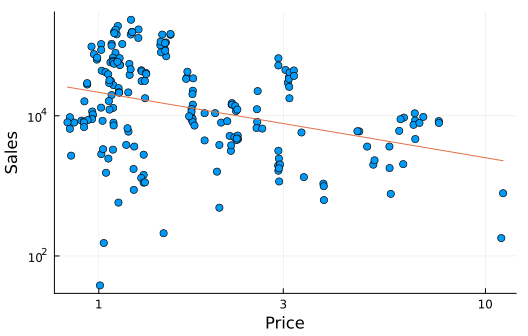
\includegraphics{./demand_estimation_1_files/figure-pdf/cell-16-output-1.svg}

}

\end{figure}

\begin{Shaded}
\begin{Highlighting}[]
\FunctionTok{describe}\NormalTok{(data[}\OperatorTok{:}\NormalTok{, [}\OperatorTok{:}\NormalTok{Sales, }\OperatorTok{:}\NormalTok{price, }\OperatorTok{:}\NormalTok{FuelEfficiency, }\OperatorTok{:}\NormalTok{size, }\OperatorTok{:}\NormalTok{hppw]])}
\end{Highlighting}
\end{Shaded}

\begin{tabular}{r|ccccccc}
    & variable & mean & min & median & max & nmissing & eltype\\
    \hline
    & Symbol & Float64 & Real & Float64 & Real & Int64 & DataType\\
    \hline
    1 & Sales & 24586.4 & 10 & 8544.0 & 317675 & 0 & Int64 \\
    2 & price & 2.53047 & 0.705176 & 2.05042 & 12.6265 & 0 & Float64 \\
    3 & FuelEfficiency & 16.1597 & 5.5 & 15.4 & 40.8 & 0 & Float64 \\
    4 & size & 11.5053 & 5.909 & 11.4725 & 19.1548 & 0 & Float64 \\
    5 & hppw & 0.0991312 & 0.045 & 0.0926829 & 0.323864 & 0 & Float64 \\
\end{tabular}

\begin{Shaded}
\begin{Highlighting}[]
\NormalTok{data[!, }\OperatorTok{:}\NormalTok{logit\_share] }\OperatorTok{=} \FunctionTok{log}\NormalTok{.(data[}\OperatorTok{:}\NormalTok{, }\OperatorTok{:}\NormalTok{share]) }\OperatorTok{.{-}} \FunctionTok{log}\NormalTok{.(data[}\OperatorTok{:}\NormalTok{, }\OperatorTok{:}\NormalTok{share0]);}
\end{Highlighting}
\end{Shaded}

\begin{Shaded}
\begin{Highlighting}[]
\NormalTok{ols\_res }\OperatorTok{=} \FunctionTok{reg}\NormalTok{(data, }\PreprocessorTok{@formula}\NormalTok{(logit\_share }\OperatorTok{\textasciitilde{}}\NormalTok{ price }\OperatorTok{+}\NormalTok{ hppw }\OperatorTok{+}\NormalTok{ FuelEfficiency }\OperatorTok{+}\NormalTok{ size), Vcov.}\FunctionTok{robust}\NormalTok{());}
\NormalTok{iv\_BLP\_res }\OperatorTok{=} \FunctionTok{reg}\NormalTok{(}
\NormalTok{    data, }
    \PreprocessorTok{@formula}\NormalTok{(logit\_share }\OperatorTok{\textasciitilde{}}\NormalTok{ (}
\NormalTok{        price }\OperatorTok{\textasciitilde{}}\NormalTok{ iv\_BLP\_own\_hppw }\OperatorTok{+}\NormalTok{ iv\_BLP\_own\_FuelEfficiency }\OperatorTok{+}\NormalTok{ iv\_BLP\_own\_size }\OperatorTok{+} 
\NormalTok{            iv\_BLP\_other\_hppw }\OperatorTok{+}\NormalTok{ iv\_BLP\_other\_FuelEfficiency }\OperatorTok{+}\NormalTok{ iv\_BLP\_other\_size}
\NormalTok{    ) }\OperatorTok{+}\NormalTok{ hppw }\OperatorTok{+}\NormalTok{ FuelEfficiency }\OperatorTok{+}\NormalTok{ size),}
\NormalTok{    Vcov.}\FunctionTok{robust}\NormalTok{()}
\NormalTok{);}
\NormalTok{iv\_GH\_res }\OperatorTok{=} \FunctionTok{reg}\NormalTok{(}
\NormalTok{    data, }
    \PreprocessorTok{@formula}\NormalTok{(logit\_share }\OperatorTok{\textasciitilde{}}\NormalTok{ (}
\NormalTok{        price }\OperatorTok{\textasciitilde{}}\NormalTok{ iv\_GH\_own\_hppw }\OperatorTok{+}\NormalTok{ iv\_GH\_own\_FuelEfficiency }\OperatorTok{+}\NormalTok{ iv\_GH\_own\_size }\OperatorTok{+} 
\NormalTok{            iv\_GH\_other\_hppw }\OperatorTok{+}\NormalTok{ iv\_GH\_other\_FuelEfficiency }\OperatorTok{+}\NormalTok{ iv\_GH\_other\_size}
\NormalTok{    ) }\OperatorTok{+}\NormalTok{ hppw }\OperatorTok{+}\NormalTok{ FuelEfficiency }\OperatorTok{+}\NormalTok{ size),}
\NormalTok{    Vcov.}\FunctionTok{robust}\NormalTok{(),}
\NormalTok{    save }\OperatorTok{=} \ConstantTok{true}
\NormalTok{);}
\end{Highlighting}
\end{Shaded}

\begin{Shaded}
\begin{Highlighting}[]
\FunctionTok{regtable}\NormalTok{(ols\_res, iv\_BLP\_res, iv\_GH\_res)}
\end{Highlighting}
\end{Shaded}

\begin{verbatim}

--------------------------------------------------------------
                                       logit_share            
                          ------------------------------------
                                 (1)          (2)          (3)
--------------------------------------------------------------
(Intercept)               -12.255***   -12.323***   -12.973***
                             (0.365)      (0.382)      (0.393)
price                      -0.255***    -0.283***    -0.552***
                             (0.026)      (0.067)      (0.080)
hppw                          -0.654        0.213      8.426**
                             (1.284)      (2.298)      (2.638)
FuelEfficiency              0.130***     0.130***     0.127***
                             (0.010)      (0.010)      (0.010)
size                        0.182***     0.187***     0.236***
                             (0.019)      (0.021)      (0.022)
--------------------------------------------------------------
Estimator                        OLS           IV           IV
--------------------------------------------------------------
N                              1,823        1,823        1,823
R2                             0.222        0.222        0.180
Within-R2                                                     
First-stage F statistic                    33.926       51.583
--------------------------------------------------------------
\end{verbatim}

\begin{Shaded}
\begin{Highlighting}[]
\NormalTok{iv1st\_BLP\_res }\OperatorTok{=} \FunctionTok{reg}\NormalTok{(}
\NormalTok{    data, }
    \PreprocessorTok{@formula}\NormalTok{(price }\OperatorTok{\textasciitilde{}}\NormalTok{ hppw }\OperatorTok{+}\NormalTok{ FuelEfficiency }\OperatorTok{+}\NormalTok{ size }\OperatorTok{+}
\NormalTok{            iv\_BLP\_own\_hppw }\OperatorTok{+}\NormalTok{ iv\_BLP\_own\_FuelEfficiency }\OperatorTok{+}\NormalTok{ iv\_BLP\_own\_size }\OperatorTok{+} 
\NormalTok{            iv\_BLP\_other\_hppw }\OperatorTok{+}\NormalTok{ iv\_BLP\_other\_FuelEfficiency }\OperatorTok{+}\NormalTok{ iv\_BLP\_other\_size}
\NormalTok{        ),}
\NormalTok{    Vcov.}\FunctionTok{robust}\NormalTok{()}
\NormalTok{);}
\NormalTok{iv1st\_GH\_res }\OperatorTok{=} \FunctionTok{reg}\NormalTok{(}
\NormalTok{    data, }
    \PreprocessorTok{@formula}\NormalTok{(price }\OperatorTok{\textasciitilde{}}\NormalTok{ hppw }\OperatorTok{+}\NormalTok{ FuelEfficiency }\OperatorTok{+}\NormalTok{ size }\OperatorTok{+}
\NormalTok{            iv\_GH\_own\_hppw }\OperatorTok{+}\NormalTok{ iv\_GH\_own\_FuelEfficiency }\OperatorTok{+}\NormalTok{ iv\_GH\_own\_size }\OperatorTok{+} 
\NormalTok{            iv\_GH\_other\_hppw }\OperatorTok{+}\NormalTok{ iv\_GH\_other\_FuelEfficiency }\OperatorTok{+}\NormalTok{ iv\_GH\_other\_size}
\NormalTok{        ),}
\NormalTok{    Vcov.}\FunctionTok{robust}\NormalTok{()}
\NormalTok{);}
\end{Highlighting}
\end{Shaded}

\begin{Shaded}
\begin{Highlighting}[]
\FunctionTok{regtable}\NormalTok{(iv1st\_BLP\_res, iv1st\_GH\_res)}
\end{Highlighting}
\end{Shaded}

\begin{verbatim}

---------------------------------------------------
                                      price        
                              ---------------------
                                    (1)         (2)
---------------------------------------------------
(Intercept)                      -3.159    -1.325**
                                (1.685)     (0.423)
hppw                          28.749***   23.508***
                                (0.993)     (1.547)
FuelEfficiency                   -0.011   -0.072***
                                (0.008)     (0.014)
size                           0.202***    0.189***
                                (0.015)     (0.020)
iv_BLP_own_hppw                 -0.728*            
                                (0.336)            
iv_BLP_own_FuelEfficiency     -0.007***            
                                (0.001)            
iv_BLP_own_size                0.013***            
                                (0.004)            
iv_BLP_other_hppw                 0.165            
                                (0.255)            
iv_BLP_other_FuelEfficiency     0.001**            
                                (0.000)            
iv_BLP_other_size                -0.002            
                                (0.003)            
iv_GH_own_hppw                            -1.889***
                                            (0.439)
iv_GH_own_FuelEfficiency                      0.000
                                            (0.000)
iv_GH_own_size                            -0.001***
                                            (0.000)
iv_GH_other_hppw                           0.423***
                                            (0.096)
iv_GH_other_FuelEfficiency                 0.000***
                                            (0.000)
iv_GH_other_size                           0.000***
                                            (0.000)
---------------------------------------------------
N                                 1,823       1,823
R2                                0.616       0.623
---------------------------------------------------
\end{verbatim}

\begin{Shaded}
\begin{Highlighting}[]
\NormalTok{data[!, }\OperatorTok{:}\NormalTok{own\_elas\_ols]   }\OperatorTok{=}\NormalTok{ ols\_res.coef[ols\_res.coefnames }\OperatorTok{.==} \StringTok{"price"}\NormalTok{] }\OperatorTok{.*}\NormalTok{ data[}\OperatorTok{:}\NormalTok{, }\OperatorTok{:}\NormalTok{price] }\OperatorTok{.*}\NormalTok{ (}\FloatTok{1} \OperatorTok{.{-}}\NormalTok{ data[}\OperatorTok{:}\NormalTok{, }\OperatorTok{:}\NormalTok{share]);}
\NormalTok{data[!, }\OperatorTok{:}\NormalTok{own\_elas\_ivblp] }\OperatorTok{=}\NormalTok{ iv\_BLP\_res.coef[iv\_BLP\_res.coefnames }\OperatorTok{.==} \StringTok{"price"}\NormalTok{] }\OperatorTok{.*}\NormalTok{ data[}\OperatorTok{:}\NormalTok{, }\OperatorTok{:}\NormalTok{price] }\OperatorTok{.*}\NormalTok{ (}\FloatTok{1} \OperatorTok{.{-}}\NormalTok{ data[}\OperatorTok{:}\NormalTok{, }\OperatorTok{:}\NormalTok{share]);}
\NormalTok{data[!, }\OperatorTok{:}\NormalTok{own\_elas\_ivgh]  }\OperatorTok{=}\NormalTok{ iv\_GH\_res.coef[iv\_GH\_res.coefnames }\OperatorTok{.==} \StringTok{"price"}\NormalTok{] }\OperatorTok{.*}\NormalTok{ data[}\OperatorTok{:}\NormalTok{, }\OperatorTok{:}\NormalTok{price] }\OperatorTok{.*}\NormalTok{ (}\FloatTok{1} \OperatorTok{.{-}}\NormalTok{ data[}\OperatorTok{:}\NormalTok{, }\OperatorTok{:}\NormalTok{share]);}
\end{Highlighting}
\end{Shaded}

\begin{Shaded}
\begin{Highlighting}[]
\FunctionTok{describe}\NormalTok{(data[}\OperatorTok{:}\NormalTok{, }\StringTok{r"\^{}own\_elas"}\NormalTok{])}
\end{Highlighting}
\end{Shaded}

\begin{tabular}{r|ccccccc}
    & variable & mean & min & median & max & nmissing & eltype\\
    \hline
    & Symbol & Float64 & Float64 & Float64 & Float64 & Int64 & DataType\\
    \hline
    1 & own\_elas\_ols & -0.645328 & -3.22104 & -0.522324 & -0.179892 & 0 & Float64 \\
    2 & own\_elas\_ivblp & -0.717085 & -3.5792 & -0.580404 & -0.199895 & 0 & Float64 \\
    3 & own\_elas\_ivgh & -1.3967 & -6.9714 & -1.13048 & -0.389346 & 0 & Float64 \\
\end{tabular}

\begin{Shaded}
\begin{Highlighting}[]
\NormalTok{dt\_application }\OperatorTok{=}\NormalTok{ data[}\OperatorTok{:}\NormalTok{, [}\OperatorTok{:}\NormalTok{NameID, }\OperatorTok{:}\NormalTok{year, }\OperatorTok{:}\NormalTok{Sales, }\OperatorTok{:}\NormalTok{price, }\OperatorTok{:}\NormalTok{FuelEfficiency, }\OperatorTok{:}\NormalTok{size, }\OperatorTok{:}\NormalTok{hppw, }\OperatorTok{:}\NormalTok{HH, }\OperatorTok{:}\NormalTok{share]];}
\NormalTok{dt\_application[!, }\OperatorTok{:}\NormalTok{xi\_fit] }\OperatorTok{=}\NormalTok{ iv\_GH\_res.residuals;}
\end{Highlighting}
\end{Shaded}

\begin{Shaded}
\begin{Highlighting}[]
\NormalTok{NameID\_target }\OperatorTok{=} \FloatTok{197}
\NormalTok{dt\_application[(dt\_application.year }\OperatorTok{.==} \FloatTok{2016}\NormalTok{) }\OperatorTok{.\&}\NormalTok{ (dt\_application.NameID }\OperatorTok{.==}\NormalTok{ NameID\_target), }\OperatorTok{:}\NormalTok{]}
\end{Highlighting}
\end{Shaded}

\begin{tabular}{r|cccccccccc}
    & NameID & year & Sales & price & FuelEfficiency & size & hppw & HH & share & \\
    \hline
    & Int64? & Int64 & Int64 & Float64 & Float64 & Float64 & Float64 & Int64? & Float64 & \\
    \hline
    1 & 197 & 2016 & 37069 & 3.198 & 11.6 & 17.0944 & 0.0947917 & 56950757 & 0.000650896 & $\dots$ \\
\end{tabular}

\begin{Shaded}
\begin{Highlighting}[]
\KeywordTok{function} \FunctionTok{f\_share}\NormalTok{(}
\NormalTok{        price\_cand,}
\NormalTok{        year, }
\NormalTok{        NameID\_target,}
\NormalTok{        dt,}
\NormalTok{        est\_res}
\NormalTok{    )}
    
\NormalTok{    dt }\OperatorTok{=}\NormalTok{ dt[dt.year }\OperatorTok{.==}\NormalTok{ year, }\OperatorTok{:}\NormalTok{]}
\NormalTok{    dt[!, }\OperatorTok{:}\NormalTok{temp\_price] }\OperatorTok{=}\NormalTok{ dt[}\OperatorTok{:}\NormalTok{, }\OperatorTok{:}\NormalTok{price]}
\NormalTok{    dt[(dt[}\OperatorTok{:}\NormalTok{, }\OperatorTok{:}\NormalTok{NameID] }\OperatorTok{.==}\NormalTok{ NameID\_target), }\OperatorTok{:}\NormalTok{temp\_price] }\OperatorTok{.=}\NormalTok{ price\_cand}
\NormalTok{    dt[!, }\OperatorTok{:}\NormalTok{delta] }\OperatorTok{=}\NormalTok{ (}
\NormalTok{        est\_res.coef[est\_res.coefnames }\OperatorTok{.==} \StringTok{"(Intercept)"}\NormalTok{] }\OperatorTok{.+}
\NormalTok{        est\_res.coef[est\_res.coefnames }\OperatorTok{.==} \StringTok{"hppw"}\NormalTok{] }\OperatorTok{.*}\NormalTok{ dt[}\OperatorTok{:}\NormalTok{, }\OperatorTok{:}\NormalTok{hppw] }\OperatorTok{.+}
\NormalTok{        est\_res.coef[est\_res.coefnames }\OperatorTok{.==} \StringTok{"FuelEfficiency"}\NormalTok{] }\OperatorTok{.*}\NormalTok{ dt[}\OperatorTok{:}\NormalTok{, }\OperatorTok{:}\NormalTok{FuelEfficiency] }\OperatorTok{.+}
\NormalTok{        est\_res.coef[est\_res.coefnames }\OperatorTok{.==} \StringTok{"size"}\NormalTok{] }\OperatorTok{.*}\NormalTok{ dt[}\OperatorTok{:}\NormalTok{, }\OperatorTok{:}\NormalTok{size] }\OperatorTok{.+}
\NormalTok{        est\_res.coef[est\_res.coefnames }\OperatorTok{.==} \StringTok{"price"}\NormalTok{] }\OperatorTok{.*}\NormalTok{ dt[}\OperatorTok{:}\NormalTok{, }\OperatorTok{:}\NormalTok{temp\_price] }\OperatorTok{.+}
\NormalTok{        dt[}\OperatorTok{:}\NormalTok{, }\OperatorTok{:}\NormalTok{xi\_fit]}
\NormalTok{    )}
\NormalTok{    dt[!, }\OperatorTok{:}\NormalTok{denom] }\OperatorTok{.=} \FloatTok{1} \OperatorTok{.+} \FunctionTok{sum}\NormalTok{(}\FunctionTok{exp}\NormalTok{.(dt[}\OperatorTok{:}\NormalTok{, }\OperatorTok{:}\NormalTok{delta]))}
\NormalTok{    dt[!, }\OperatorTok{:}\NormalTok{pred\_sales] }\OperatorTok{=} \FunctionTok{exp}\NormalTok{.(dt[}\OperatorTok{:}\NormalTok{, }\OperatorTok{:}\NormalTok{delta]) }\OperatorTok{./}\NormalTok{ dt[}\OperatorTok{:}\NormalTok{, }\OperatorTok{:}\NormalTok{denom] }\OperatorTok{.*}\NormalTok{ dt[}\OperatorTok{:}\NormalTok{, }\OperatorTok{:}\NormalTok{HH]}
\NormalTok{    dt }\OperatorTok{=}\NormalTok{ dt[dt.NameID }\OperatorTok{.==}\NormalTok{ NameID\_target, }\OperatorTok{:}\NormalTok{]}
    
    \ControlFlowTok{return}\NormalTok{ dt.pred\_sales[}\FloatTok{1}\NormalTok{]}
    
\KeywordTok{end}
\end{Highlighting}
\end{Shaded}

\begin{verbatim}
f_share (generic function with 1 method)
\end{verbatim}

\begin{Shaded}
\begin{Highlighting}[]
\NormalTok{pricevec }\OperatorTok{=} \FunctionTok{range}\NormalTok{(}\FloatTok{0.3}\NormalTok{, }\FloatTok{5}\NormalTok{, step }\OperatorTok{=} \FloatTok{0.05}\NormalTok{);}
\NormalTok{quantvec }\OperatorTok{=} \FunctionTok{f\_share}\NormalTok{.(pricevec, }\FloatTok{2016}\NormalTok{, NameID\_target, }\FunctionTok{Ref}\NormalTok{(dt\_application), }\FunctionTok{Ref}\NormalTok{(iv\_GH\_res));}
\end{Highlighting}
\end{Shaded}

\begin{Shaded}
\begin{Highlighting}[]
\FunctionTok{plot}\NormalTok{(quantvec, pricevec, xticks }\OperatorTok{=}\NormalTok{ [}\FloatTok{50000}\NormalTok{, }\FloatTok{100000}\NormalTok{, }\FloatTok{150000}\NormalTok{], legend }\OperatorTok{=} \ConstantTok{false}\NormalTok{)}
\FunctionTok{xlabel!}\NormalTok{(}\StringTok{"Sales"}\NormalTok{)}
\FunctionTok{ylabel!}\NormalTok{(}\StringTok{"Price (million JPY)"}\NormalTok{)}
\end{Highlighting}
\end{Shaded}

\begin{figure}[H]

{\centering 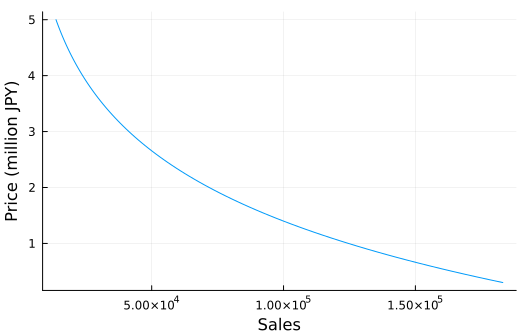
\includegraphics{./demand_estimation_1_files/figure-pdf/cell-29-output-1.svg}

}

\end{figure}

\begin{Shaded}
\begin{Highlighting}[]
\FunctionTok{plot}\NormalTok{(pricevec, pricevec }\OperatorTok{.*}\NormalTok{ quantvec }\OperatorTok{/} \FloatTok{1000}\NormalTok{, legend }\OperatorTok{=} \ConstantTok{false}\NormalTok{)}
\FunctionTok{xlabel!}\NormalTok{(}\StringTok{"Price (million JPY)"}\NormalTok{)}
\FunctionTok{ylabel!}\NormalTok{(}\StringTok{"Revenue (billion JPY)"}\NormalTok{)}
\end{Highlighting}
\end{Shaded}

\begin{figure}[H]

{\centering 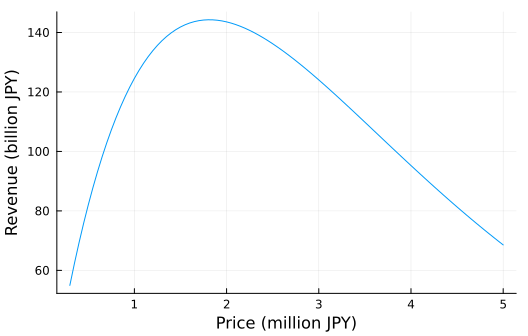
\includegraphics{./demand_estimation_1_files/figure-pdf/cell-30-output-1.svg}

}

\end{figure}

\begin{Shaded}
\begin{Highlighting}[]
\NormalTok{opt\_res }\OperatorTok{=} \FunctionTok{optimize}\NormalTok{(}
\NormalTok{    x }\OperatorTok{{-}\textgreater{}} \OperatorTok{{-}} \FunctionTok{f\_share}\NormalTok{(x[}\FloatTok{1}\NormalTok{], }\FloatTok{2016}\NormalTok{, NameID\_target, dt\_application, iv\_GH\_res) }\OperatorTok{*}\NormalTok{ x[}\FloatTok{1}\NormalTok{],}
\NormalTok{    [}\FloatTok{1.0}\NormalTok{]}
\NormalTok{);}

\PreprocessorTok{@printf}\NormalTok{(}\StringTok{"Revenue{-}maximizing price: \%.3f }\SpecialCharTok{\textbackslash{}n}\StringTok{"}\NormalTok{, opt\_res.minimizer[}\FloatTok{1}\NormalTok{])}
\PreprocessorTok{@printf}\NormalTok{(}\StringTok{"Max revenue : \%.3f"}\NormalTok{, }\OperatorTok{{-}}\NormalTok{opt\_res.minimum)}
\end{Highlighting}
\end{Shaded}

\begin{verbatim}
Revenue-maximizing price: 1.814 
Max revenue : 144273.836
\end{verbatim}

\bookmarksetup{startatroot}

\hypertarget{ux9700ux8981ux30e2ux30c7ux30ebux306eux63a8ux5b9aux57faux790eux7de8-2}{%
\chapter{需要モデルの推定(基礎編
2)}\label{ux9700ux8981ux30e2ux30c7ux30ebux306eux63a8ux5b9aux57faux790eux7de8-2}}

\begin{Shaded}
\begin{Highlighting}[]
\ImportTok{using} \BuiltInTok{CSV}
\ImportTok{using} \BuiltInTok{DataFrames}
\ImportTok{using} \BuiltInTok{StringEncodings}
\ImportTok{using} \BuiltInTok{FixedEffectModels}
\ImportTok{using} \BuiltInTok{RegressionTables}
\ImportTok{using} \BuiltInTok{Plots}
\ImportTok{using} \BuiltInTok{LinearAlgebra}
\ImportTok{using} \BuiltInTok{Statistics}
\ImportTok{using} \BuiltInTok{Optim}
\ImportTok{using} \BuiltInTok{Printf}
\ImportTok{using} \BuiltInTok{ForwardDiff}
\ImportTok{using} \BuiltInTok{Random}
\ImportTok{using} \BuiltInTok{GLM}
\ImportTok{using} \BuiltInTok{Serialization}
\end{Highlighting}
\end{Shaded}

\begin{Shaded}
\begin{Highlighting}[]
\NormalTok{data }\OperatorTok{=}\NormalTok{ CSV.}\FunctionTok{File}\NormalTok{(}
    \FunctionTok{open}\NormalTok{(read, }\StringTok{"data/demand\_estimation/CleanData\_20180222.csv"}\NormalTok{, enc}\StringTok{"shift{-}jis"}\NormalTok{),}
\NormalTok{    missingstring }\OperatorTok{=}\NormalTok{ [}\StringTok{"NA"}\NormalTok{, }\StringTok{""}\NormalTok{],}
\NormalTok{    ) }\OperatorTok{|\textgreater{}}\NormalTok{ DataFrame}
\FunctionTok{first}\NormalTok{(}\FunctionTok{select}\NormalTok{(data, }\FunctionTok{Not}\NormalTok{([}\OperatorTok{:}\NormalTok{base\_color, }\OperatorTok{:}\NormalTok{option\_color])), }\FloatTok{5}\NormalTok{)}
\end{Highlighting}
\end{Shaded}

\begin{tabular}{r|ccccccccc}
    & Maker & Type & Name & Year & Sales & comment & Model & Year\_true & \\
    \hline
    & String15 & String7 & String31 & Int64 & Int64 & String? & String & Int64 & \\
    \hline
    1 & Audi & Foreign & A1シリーズ & 2011 & 4206 & \emph{missing} & 1.4 TFSI & 2011 & $\dots$ \\
    2 & Audi & Foreign & A1シリーズ & 2012 & 4502 & \emph{missing} & 1.4 TFSI & 2012 & $\dots$ \\
    3 & Audi & Foreign & A1シリーズ & 2013 & 5071 & \emph{missing} & 1.4 TFSI & 2012 & $\dots$ \\
    4 & Audi & Foreign & A3シリーズ & 2006 & 4830 & \emph{missing} & アトラクション & 2006 & $\dots$ \\
    5 & Audi & Foreign & A3シリーズ & 2007 & 3874 & \emph{missing} & アトラクション & 2007 & $\dots$ \\
\end{tabular}

\begin{Shaded}
\begin{Highlighting}[]
\NormalTok{dataHH }\OperatorTok{=}\NormalTok{ CSV.}\FunctionTok{read}\NormalTok{(}\StringTok{"data/demand\_estimation/HHsize.csv"}\NormalTok{, DataFrame)}
\NormalTok{dataHH[!, }\OperatorTok{:}\NormalTok{HH] }\OperatorTok{=} \FunctionTok{parse}\NormalTok{.(}\DataTypeTok{Int}\NormalTok{, }\FunctionTok{replace}\NormalTok{.(dataHH.HH, }\StringTok{","} \OperatorTok{=\textgreater{}} \StringTok{""}\NormalTok{))}
\FunctionTok{first}\NormalTok{(dataHH, }\FloatTok{5}\NormalTok{)}
\end{Highlighting}
\end{Shaded}

\begin{tabular}{r|cc}
    & year & HH\\
    \hline
    & Int64 & Int64\\
    \hline
    1 & 1975 & 33310006 \\
    2 & 1976 & 33911052 \\
    3 & 1977 & 34380314 \\
    4 & 1978 & 34858696 \\
    5 & 1979 & 35350173 \\
\end{tabular}

\begin{Shaded}
\begin{Highlighting}[]
\NormalTok{dataCPI }\OperatorTok{=}\NormalTok{ CSV.}\FunctionTok{File}\NormalTok{(}
    \FunctionTok{open}\NormalTok{(read, }\StringTok{"data/demand\_estimation/zni2015s.csv"}\NormalTok{, enc}\StringTok{"shift{-}jis"}\NormalTok{), }
\NormalTok{    select }\OperatorTok{=} \FloatTok{1}\OperatorTok{:}\FloatTok{2}\NormalTok{,}
\NormalTok{    skipto }\OperatorTok{=} \FloatTok{7}
\NormalTok{    ) }\OperatorTok{|\textgreater{}}\NormalTok{ DataFrame}
\FunctionTok{rename!}\NormalTok{(dataCPI, }\StringTok{"類・品目"} \OperatorTok{=\textgreater{}} \StringTok{"year"}\NormalTok{, }\StringTok{"総合"} \OperatorTok{=\textgreater{}} \StringTok{"CPI"}\NormalTok{)}
\FunctionTok{first}\NormalTok{(dataCPI, }\FloatTok{5}\NormalTok{)}
\end{Highlighting}
\end{Shaded}

\begin{tabular}{r|cc}
    & year & CPI\\
    \hline
    & Int64 & Float64\\
    \hline
    1 & 1970 & 31.5 \\
    2 & 1971 & 33.5 \\
    3 & 1972 & 35.2 \\
    4 & 1973 & 39.3 \\
    5 & 1974 & 48.4 \\
\end{tabular}

\begin{Shaded}
\begin{Highlighting}[]
\NormalTok{data }\OperatorTok{=}\NormalTok{ data[!, [}
        \OperatorTok{:}\NormalTok{Maker, }\OperatorTok{:}\DataTypeTok{Type}\NormalTok{, }\OperatorTok{:}\NormalTok{Name, }\OperatorTok{:}\NormalTok{Year, }\OperatorTok{:}\NormalTok{Sales, }
        \OperatorTok{:}\NormalTok{Model, }\OperatorTok{:}\NormalTok{price, }\OperatorTok{:}\NormalTok{kata, }\OperatorTok{:}\NormalTok{weight, }\OperatorTok{:}\NormalTok{FuelEfficiency, }
        \OperatorTok{:}\NormalTok{HorsePower, }\OperatorTok{:}\NormalTok{overall\_length, }\OperatorTok{:}\NormalTok{overall\_width, }\OperatorTok{:}\NormalTok{overall\_height}
\NormalTok{        ]]}
\FunctionTok{rename!}\NormalTok{(data, }\StringTok{"Year"} \OperatorTok{=\textgreater{}} \StringTok{"year"}\NormalTok{)}
\NormalTok{data }\OperatorTok{=} \FunctionTok{leftjoin}\NormalTok{(data, dataHH, on }\OperatorTok{=} \OperatorTok{:}\NormalTok{year)}
\NormalTok{data }\OperatorTok{=} \FunctionTok{leftjoin}\NormalTok{(data, dataCPI, on }\OperatorTok{=} \OperatorTok{:}\NormalTok{year)}
\FunctionTok{first}\NormalTok{(data, }\FloatTok{5}\NormalTok{)}
\end{Highlighting}
\end{Shaded}

\begin{tabular}{r|ccccccccc}
    & Maker & Type & Name & year & Sales & Model & price & kata & \\
    \hline
    & String15 & String7 & String31 & Int64 & Int64 & String & Float64 & String15 & \\
    \hline
    1 & Audi & Foreign & A1シリーズ & 2011 & 4206 & 1.4 TFSI & 289.0 & DBA-8XCAX & $\dots$ \\
    2 & Audi & Foreign & A1シリーズ & 2012 & 4502 & 1.4 TFSI & 273.0 & DBA-8XCAX & $\dots$ \\
    3 & Audi & Foreign & A1シリーズ & 2013 & 5071 & 1.4 TFSI & 273.0 & DBA-8XCAX & $\dots$ \\
    4 & Audi & Foreign & A3シリーズ & 2006 & 4830 & アトラクション & 284.0 & GH-8PBSE & $\dots$ \\
    5 & Audi & Foreign & A3シリーズ & 2007 & 3874 & アトラクション & 286.0 & GH-8PBSE & $\dots$ \\
\end{tabular}

\begin{Shaded}
\begin{Highlighting}[]
\FunctionTok{dropmissing!}\NormalTok{(data, }\OperatorTok{:}\NormalTok{FuelEfficiency);}
\NormalTok{cpi2016 }\OperatorTok{=}\NormalTok{ dataCPI[dataCPI.year }\OperatorTok{.==} \FloatTok{2016}\NormalTok{, }\StringTok{"CPI"}\NormalTok{][}\FloatTok{1}\NormalTok{]}
\NormalTok{data[!, }\OperatorTok{:}\NormalTok{price] }\OperatorTok{=}\NormalTok{ data.price }\OperatorTok{./}\NormalTok{ (data.CPI }\OperatorTok{/}\NormalTok{ cpi2016) }\OperatorTok{/} \FloatTok{100}\NormalTok{;}
\NormalTok{data[!, }\OperatorTok{:}\NormalTok{size] }\OperatorTok{=}\NormalTok{ (data[}\OperatorTok{:}\NormalTok{, }\OperatorTok{:}\NormalTok{overall\_length] }\OperatorTok{/} \FloatTok{1000}\NormalTok{) }\OperatorTok{.*}\NormalTok{ (data[}\OperatorTok{:}\NormalTok{, }\OperatorTok{:}\NormalTok{overall\_width] }\OperatorTok{/} \FloatTok{1000}\NormalTok{) }\OperatorTok{.*}\NormalTok{ (data[}\OperatorTok{:}\NormalTok{, }\OperatorTok{:}\NormalTok{overall\_height] }\OperatorTok{/} \FloatTok{1000}\NormalTok{);}
\NormalTok{data[!, }\OperatorTok{:}\NormalTok{hppw] }\OperatorTok{=}\NormalTok{ data[}\OperatorTok{:}\NormalTok{, }\OperatorTok{:}\NormalTok{HorsePower] }\OperatorTok{./}\NormalTok{ data[}\OperatorTok{:}\NormalTok{, }\OperatorTok{:}\NormalTok{weight];}

\NormalTok{unique\_name }\OperatorTok{=} \FunctionTok{unique}\NormalTok{(data[!, [}\OperatorTok{:}\NormalTok{Name]])}
\NormalTok{unique\_name[!, }\OperatorTok{:}\NormalTok{NameID] }\OperatorTok{=} \FunctionTok{rownumber}\NormalTok{.(}\FunctionTok{eachrow}\NormalTok{(unique\_name))}
\NormalTok{data }\OperatorTok{=} \FunctionTok{leftjoin}\NormalTok{(data, unique\_name, on }\OperatorTok{=} \OperatorTok{:}\NormalTok{Name);}

\NormalTok{data }\OperatorTok{=} \FunctionTok{transform}\NormalTok{(}
    \FunctionTok{groupby}\NormalTok{(data, }\OperatorTok{:}\NormalTok{year),}
    \OperatorTok{:}\NormalTok{Sales }\OperatorTok{=\textgreater{}}\NormalTok{ sum }\OperatorTok{=\textgreater{}} \OperatorTok{:}\NormalTok{inside\_total}
\NormalTok{);}
\NormalTok{data[!, }\OperatorTok{:}\NormalTok{outside\_total] }\OperatorTok{=}\NormalTok{ data.HH }\OperatorTok{.{-}}\NormalTok{ data.inside\_total;}
\NormalTok{data[!, }\OperatorTok{:}\NormalTok{share] }\OperatorTok{=}\NormalTok{ data.Sales }\OperatorTok{./}\NormalTok{ data.HH;}
\NormalTok{data[!, }\OperatorTok{:}\NormalTok{share0] }\OperatorTok{=}\NormalTok{ data.outside\_total }\OperatorTok{./}\NormalTok{ data.HH;}
\FunctionTok{transform!}\NormalTok{(}
    \FunctionTok{groupby}\NormalTok{(data, [}\OperatorTok{:}\NormalTok{year, }\OperatorTok{:}\NormalTok{Maker]),}
\NormalTok{    [}\OperatorTok{:}\NormalTok{hppw, }\OperatorTok{:}\NormalTok{FuelEfficiency, }\OperatorTok{:}\NormalTok{size] }\OperatorTok{.=\textgreater{}}\NormalTok{ sum }\OperatorTok{.=\textgreater{}}\NormalTok{ [}\OperatorTok{:}\NormalTok{hppw\_sum\_own, }\OperatorTok{:}\NormalTok{FuelEfficiency\_sum\_own, }\OperatorTok{:}\NormalTok{size\_sum\_own],}
\NormalTok{    [}\OperatorTok{:}\NormalTok{hppw, }\OperatorTok{:}\NormalTok{FuelEfficiency, }\OperatorTok{:}\NormalTok{size] }\OperatorTok{.=\textgreater{}}\NormalTok{ (x }\OperatorTok{{-}\textgreater{}} \FunctionTok{sum}\NormalTok{(x}\OperatorTok{.\^{}}\FloatTok{2}\NormalTok{)) }\OperatorTok{.=\textgreater{}}\NormalTok{ [}\OperatorTok{:}\NormalTok{hppw\_sqr\_sum\_own, }\OperatorTok{:}\NormalTok{FuelEfficiency\_sqr\_sum\_own, }\OperatorTok{:}\NormalTok{size\_sqr\_sum\_own],}
\NormalTok{    nrow }\OperatorTok{=\textgreater{}} \StringTok{"group\_n"}
\NormalTok{);}
\FunctionTok{transform!}\NormalTok{(}
    \FunctionTok{groupby}\NormalTok{(data, [}\OperatorTok{:}\NormalTok{year]),}
\NormalTok{    [}\OperatorTok{:}\NormalTok{hppw, }\OperatorTok{:}\NormalTok{FuelEfficiency, }\OperatorTok{:}\NormalTok{size] }\OperatorTok{.=\textgreater{}}\NormalTok{ sum }\OperatorTok{.=\textgreater{}}\NormalTok{ [}\OperatorTok{:}\NormalTok{hppw\_sum\_mkt, }\OperatorTok{:}\NormalTok{FuelEfficiency\_sum\_mkt, }\OperatorTok{:}\NormalTok{size\_sum\_mkt],}
\NormalTok{    [}\OperatorTok{:}\NormalTok{hppw, }\OperatorTok{:}\NormalTok{FuelEfficiency, }\OperatorTok{:}\NormalTok{size] }\OperatorTok{.=\textgreater{}}\NormalTok{ (x }\OperatorTok{{-}\textgreater{}} \FunctionTok{sum}\NormalTok{(x}\OperatorTok{.\^{}}\FloatTok{2}\NormalTok{)) }\OperatorTok{.=\textgreater{}}\NormalTok{ [}\OperatorTok{:}\NormalTok{hppw\_sqr\_sum\_mkt, }\OperatorTok{:}\NormalTok{FuelEfficiency\_sqr\_sum\_mkt, }\OperatorTok{:}\NormalTok{size\_sqr\_sum\_mkt],}
\NormalTok{    nrow }\OperatorTok{=\textgreater{}} \StringTok{"mkt\_n"}
\NormalTok{);}

\NormalTok{data[!, }\OperatorTok{:}\NormalTok{iv\_BLP\_own\_hppw]             }\OperatorTok{=}\NormalTok{ data[}\OperatorTok{:}\NormalTok{, }\OperatorTok{:}\NormalTok{hppw\_sum\_own]           }\OperatorTok{.{-}}\NormalTok{ data[}\OperatorTok{:}\NormalTok{, }\OperatorTok{:}\NormalTok{hppw];}
\NormalTok{data[!, }\OperatorTok{:}\NormalTok{iv\_BLP\_own\_FuelEfficiency]   }\OperatorTok{=}\NormalTok{ data[}\OperatorTok{:}\NormalTok{, }\OperatorTok{:}\NormalTok{FuelEfficiency\_sum\_own] }\OperatorTok{.{-}}\NormalTok{ data[}\OperatorTok{:}\NormalTok{, }\OperatorTok{:}\NormalTok{FuelEfficiency];}
\NormalTok{data[!, }\OperatorTok{:}\NormalTok{iv\_BLP\_own\_size]             }\OperatorTok{=}\NormalTok{ data[}\OperatorTok{:}\NormalTok{, }\OperatorTok{:}\NormalTok{size\_sum\_own]           }\OperatorTok{.{-}}\NormalTok{ data[}\OperatorTok{:}\NormalTok{, }\OperatorTok{:}\NormalTok{size];}
\NormalTok{data[!, }\OperatorTok{:}\NormalTok{iv\_BLP\_other\_hppw]           }\OperatorTok{=}\NormalTok{ data[}\OperatorTok{:}\NormalTok{, }\OperatorTok{:}\NormalTok{hppw\_sum\_mkt]           }\OperatorTok{.{-}}\NormalTok{ data[}\OperatorTok{:}\NormalTok{, }\OperatorTok{:}\NormalTok{hppw\_sum\_own];}
\NormalTok{data[!, }\OperatorTok{:}\NormalTok{iv\_BLP\_other\_FuelEfficiency] }\OperatorTok{=}\NormalTok{ data[}\OperatorTok{:}\NormalTok{, }\OperatorTok{:}\NormalTok{FuelEfficiency\_sum\_mkt] }\OperatorTok{.{-}}\NormalTok{ data[}\OperatorTok{:}\NormalTok{, }\OperatorTok{:}\NormalTok{FuelEfficiency\_sum\_own];}
\NormalTok{data[!, }\OperatorTok{:}\NormalTok{iv\_BLP\_other\_size]           }\OperatorTok{=}\NormalTok{ data[}\OperatorTok{:}\NormalTok{, }\OperatorTok{:}\NormalTok{size\_sum\_mkt]           }\OperatorTok{.{-}}\NormalTok{ data[}\OperatorTok{:}\NormalTok{, }\OperatorTok{:}\NormalTok{size\_sum\_own];}

\NormalTok{data[!, }\OperatorTok{:}\NormalTok{iv\_GH\_own\_hppw]             }\OperatorTok{=}\NormalTok{ (}
\NormalTok{    (data[}\OperatorTok{:}\NormalTok{, }\OperatorTok{:}\NormalTok{group\_n] }\OperatorTok{.{-}} \FloatTok{1}\NormalTok{) }\OperatorTok{.*}\NormalTok{ data[}\OperatorTok{:}\NormalTok{, }\OperatorTok{:}\NormalTok{hppw]}\OperatorTok{.\^{}}\FloatTok{2} \OperatorTok{.+} 
\NormalTok{    (data[}\OperatorTok{:}\NormalTok{, }\OperatorTok{:}\NormalTok{hppw\_sqr\_sum\_own] }\OperatorTok{.{-}}\NormalTok{ data[}\OperatorTok{:}\NormalTok{, }\OperatorTok{:}\NormalTok{hppw]}\OperatorTok{.\^{}}\FloatTok{2}\NormalTok{) }\OperatorTok{.{-}} 
    \FloatTok{2} \OperatorTok{.*}\NormalTok{ data[}\OperatorTok{:}\NormalTok{, }\OperatorTok{:}\NormalTok{hppw] }\OperatorTok{.*}\NormalTok{ (data[}\OperatorTok{:}\NormalTok{, }\OperatorTok{:}\NormalTok{hppw\_sum\_own] }\OperatorTok{.{-}}\NormalTok{ data[}\OperatorTok{:}\NormalTok{, }\OperatorTok{:}\NormalTok{hppw])}
\NormalTok{);}
\NormalTok{data[!, }\OperatorTok{:}\NormalTok{iv\_GH\_own\_FuelEfficiency]   }\OperatorTok{=}\NormalTok{ (}
\NormalTok{    (data[}\OperatorTok{:}\NormalTok{, }\OperatorTok{:}\NormalTok{group\_n] }\OperatorTok{.{-}} \FloatTok{1}\NormalTok{) }\OperatorTok{.*}\NormalTok{ data[}\OperatorTok{:}\NormalTok{, }\OperatorTok{:}\NormalTok{FuelEfficiency]}\OperatorTok{.\^{}}\FloatTok{2} \OperatorTok{.+} 
\NormalTok{    (data[}\OperatorTok{:}\NormalTok{, }\OperatorTok{:}\NormalTok{FuelEfficiency\_sqr\_sum\_own] }\OperatorTok{.{-}}\NormalTok{ data[}\OperatorTok{:}\NormalTok{, }\OperatorTok{:}\NormalTok{FuelEfficiency]}\OperatorTok{.\^{}}\FloatTok{2}\NormalTok{) }\OperatorTok{.{-}} 
    \FloatTok{2} \OperatorTok{.*}\NormalTok{ data[}\OperatorTok{:}\NormalTok{, }\OperatorTok{:}\NormalTok{FuelEfficiency] }\OperatorTok{.*}\NormalTok{ (data[}\OperatorTok{:}\NormalTok{, }\OperatorTok{:}\NormalTok{FuelEfficiency\_sum\_own] }\OperatorTok{.{-}}\NormalTok{ data[}\OperatorTok{:}\NormalTok{, }\OperatorTok{:}\NormalTok{FuelEfficiency])}
\NormalTok{);}
\NormalTok{data[!, }\OperatorTok{:}\NormalTok{iv\_GH\_own\_size]             }\OperatorTok{=}\NormalTok{ (}
\NormalTok{    (data[}\OperatorTok{:}\NormalTok{, }\OperatorTok{:}\NormalTok{group\_n] }\OperatorTok{.{-}} \FloatTok{1}\NormalTok{) }\OperatorTok{.*}\NormalTok{ data[}\OperatorTok{:}\NormalTok{, }\OperatorTok{:}\NormalTok{size]}\OperatorTok{.\^{}}\FloatTok{2} \OperatorTok{.+} 
\NormalTok{    (data[}\OperatorTok{:}\NormalTok{, }\OperatorTok{:}\NormalTok{size\_sqr\_sum\_own] }\OperatorTok{.{-}}\NormalTok{ data[}\OperatorTok{:}\NormalTok{, }\OperatorTok{:}\NormalTok{size]}\OperatorTok{.\^{}}\FloatTok{2}\NormalTok{) }\OperatorTok{.{-}} 
    \FloatTok{2} \OperatorTok{.*}\NormalTok{ data[}\OperatorTok{:}\NormalTok{, }\OperatorTok{:}\NormalTok{size] }\OperatorTok{.*}\NormalTok{ (data[}\OperatorTok{:}\NormalTok{, }\OperatorTok{:}\NormalTok{size\_sum\_own] }\OperatorTok{.{-}}\NormalTok{ data[}\OperatorTok{:}\NormalTok{, }\OperatorTok{:}\NormalTok{size])}
\NormalTok{);}
\NormalTok{data[!, }\OperatorTok{:}\NormalTok{iv\_GH\_other\_hppw]           }\OperatorTok{=}\NormalTok{ (}
\NormalTok{    (data[}\OperatorTok{:}\NormalTok{, }\OperatorTok{:}\NormalTok{mkt\_n] }\OperatorTok{.{-}}\NormalTok{ data[}\OperatorTok{:}\NormalTok{, }\OperatorTok{:}\NormalTok{group\_n]) }\OperatorTok{.*}\NormalTok{ data[}\OperatorTok{:}\NormalTok{, }\OperatorTok{:}\NormalTok{hppw]}\OperatorTok{.\^{}}\FloatTok{2} \OperatorTok{.+} 
\NormalTok{    (data[}\OperatorTok{:}\NormalTok{, }\OperatorTok{:}\NormalTok{hppw\_sqr\_sum\_mkt] }\OperatorTok{.{-}}\NormalTok{ data[}\OperatorTok{:}\NormalTok{, }\OperatorTok{:}\NormalTok{hppw\_sqr\_sum\_own]) }\OperatorTok{.{-}} 
    \FloatTok{2} \OperatorTok{.*}\NormalTok{ data[}\OperatorTok{:}\NormalTok{, }\OperatorTok{:}\NormalTok{hppw] }\OperatorTok{.*}\NormalTok{ (data[}\OperatorTok{:}\NormalTok{, }\OperatorTok{:}\NormalTok{hppw\_sum\_mkt] }\OperatorTok{.{-}}\NormalTok{ data[}\OperatorTok{:}\NormalTok{, }\OperatorTok{:}\NormalTok{hppw\_sum\_own])}
\NormalTok{);}
\NormalTok{data[!, }\OperatorTok{:}\NormalTok{iv\_GH\_other\_FuelEfficiency] }\OperatorTok{=}\NormalTok{ (}
\NormalTok{    (data[}\OperatorTok{:}\NormalTok{, }\OperatorTok{:}\NormalTok{mkt\_n] }\OperatorTok{.{-}}\NormalTok{ data[}\OperatorTok{:}\NormalTok{, }\OperatorTok{:}\NormalTok{group\_n]) }\OperatorTok{.*}\NormalTok{ data[}\OperatorTok{:}\NormalTok{, }\OperatorTok{:}\NormalTok{FuelEfficiency]}\OperatorTok{.\^{}}\FloatTok{2} \OperatorTok{.+} 
\NormalTok{    (data[}\OperatorTok{:}\NormalTok{, }\OperatorTok{:}\NormalTok{FuelEfficiency\_sqr\_sum\_mkt] }\OperatorTok{.{-}}\NormalTok{ data[}\OperatorTok{:}\NormalTok{, }\OperatorTok{:}\NormalTok{FuelEfficiency\_sqr\_sum\_own]) }\OperatorTok{.{-}} 
    \FloatTok{2} \OperatorTok{.*}\NormalTok{ data[}\OperatorTok{:}\NormalTok{, }\OperatorTok{:}\NormalTok{FuelEfficiency] }\OperatorTok{.*}\NormalTok{ (data[}\OperatorTok{:}\NormalTok{, }\OperatorTok{:}\NormalTok{FuelEfficiency\_sum\_mkt] }\OperatorTok{.{-}}\NormalTok{ data[}\OperatorTok{:}\NormalTok{, }\OperatorTok{:}\NormalTok{FuelEfficiency\_sum\_own])}
\NormalTok{);}
\NormalTok{data[!, }\OperatorTok{:}\NormalTok{iv\_GH\_other\_size]           }\OperatorTok{=}\NormalTok{ (}
\NormalTok{    (data[}\OperatorTok{:}\NormalTok{, }\OperatorTok{:}\NormalTok{mkt\_n] }\OperatorTok{.{-}}\NormalTok{ data[}\OperatorTok{:}\NormalTok{, }\OperatorTok{:}\NormalTok{group\_n]) }\OperatorTok{.*}\NormalTok{ data[}\OperatorTok{:}\NormalTok{, }\OperatorTok{:}\NormalTok{size]}\OperatorTok{.\^{}}\FloatTok{2} \OperatorTok{.+} 
\NormalTok{    (data[}\OperatorTok{:}\NormalTok{, }\OperatorTok{:}\NormalTok{size\_sqr\_sum\_mkt] }\OperatorTok{.{-}}\NormalTok{ data[}\OperatorTok{:}\NormalTok{, }\OperatorTok{:}\NormalTok{size\_sqr\_sum\_own]) }\OperatorTok{.{-}} 
    \FloatTok{2} \OperatorTok{.*}\NormalTok{ data[}\OperatorTok{:}\NormalTok{, }\OperatorTok{:}\NormalTok{size] }\OperatorTok{.*}\NormalTok{ (data[}\OperatorTok{:}\NormalTok{, }\OperatorTok{:}\NormalTok{size\_sum\_mkt] }\OperatorTok{.{-}}\NormalTok{ data[}\OperatorTok{:}\NormalTok{, }\OperatorTok{:}\NormalTok{size\_sum\_own])}
\NormalTok{);}
\end{Highlighting}
\end{Shaded}

\hypertarget{section}{%
\section{4.1}\label{section}}

\begin{Shaded}
\begin{Highlighting}[]
\NormalTok{NIPPYOautoIDvec }\OperatorTok{=}\NormalTok{ [}
    \FloatTok{260}\NormalTok{, }\FloatTok{4}\NormalTok{, }\FloatTok{76}\NormalTok{, }\FloatTok{104}\NormalTok{, }\FloatTok{64}\NormalTok{, }\FloatTok{54}\NormalTok{, }\FloatTok{152}\NormalTok{, }\FloatTok{153}\NormalTok{, }\FloatTok{71}\NormalTok{, }\FloatTok{197}\NormalTok{,}
    \FloatTok{42}\NormalTok{, }\FloatTok{45}\NormalTok{, }\FloatTok{114}\NormalTok{, }\FloatTok{208}\NormalTok{, }\FloatTok{209}\NormalTok{, }\FloatTok{77}\NormalTok{, }\FloatTok{236}\NormalTok{, }\FloatTok{58}\NormalTok{, }\FloatTok{127}\NormalTok{, }\FloatTok{187}\NormalTok{,}
    \FloatTok{79}\NormalTok{, }\FloatTok{175}\NormalTok{, }\FloatTok{19}\NormalTok{, }\FloatTok{117}\NormalTok{, }\FloatTok{216}\NormalTok{, }\FloatTok{112}\NormalTok{, }\FloatTok{256}\NormalTok{, }\FloatTok{119}\NormalTok{, }\FloatTok{37}\NormalTok{, }\FloatTok{158}
\NormalTok{];}
\NormalTok{data\_NIPPYO }\OperatorTok{=}\NormalTok{ data[}
    \FunctionTok{in}\NormalTok{(NIPPYOautoIDvec).(data[}\OperatorTok{:}\NormalTok{, }\OperatorTok{:}\NormalTok{NameID]), }
\NormalTok{    [}\OperatorTok{:}\NormalTok{year, }\OperatorTok{:}\NormalTok{share, }\OperatorTok{:}\NormalTok{NameID, }\OperatorTok{:}\NormalTok{Sales, }\OperatorTok{:}\NormalTok{price, }\OperatorTok{:}\NormalTok{hppw, }\OperatorTok{:}\NormalTok{FuelEfficiency, }\OperatorTok{:}\NormalTok{size, }\OperatorTok{:}\NormalTok{Name]}
\NormalTok{    ];}
\NormalTok{data\_NIPPYO[!, }\OperatorTok{:}\NormalTok{log\_sales] }\OperatorTok{=} \FunctionTok{log}\NormalTok{.(data\_NIPPYO[}\OperatorTok{:}\NormalTok{, }\OperatorTok{:}\NormalTok{Sales]);}
\NormalTok{data\_NIPPYO[!, }\OperatorTok{:}\NormalTok{log\_price] }\OperatorTok{=} \FunctionTok{log}\NormalTok{.(data\_NIPPYO[}\OperatorTok{:}\NormalTok{, }\OperatorTok{:}\NormalTok{price]);}
\NormalTok{data\_NIPPYO[!, }\OperatorTok{:}\NormalTok{log10\_sales] }\OperatorTok{=} \FunctionTok{log10}\NormalTok{.(data\_NIPPYO[}\OperatorTok{:}\NormalTok{, }\OperatorTok{:}\NormalTok{Sales]);}
\NormalTok{data\_NIPPYO[!, }\OperatorTok{:}\NormalTok{log10\_price] }\OperatorTok{=} \FunctionTok{log10}\NormalTok{.(data\_NIPPYO[}\OperatorTok{:}\NormalTok{, }\OperatorTok{:}\NormalTok{price]);}
\CommentTok{\#\# 4.2}
\NormalTok{data[!, }\OperatorTok{:}\NormalTok{logit\_share] }\OperatorTok{=} \FunctionTok{log}\NormalTok{.(data[}\OperatorTok{:}\NormalTok{, }\OperatorTok{:}\NormalTok{share]) }\OperatorTok{.{-}} \FunctionTok{log}\NormalTok{.(data[}\OperatorTok{:}\NormalTok{, }\OperatorTok{:}\NormalTok{share0]);}

\NormalTok{iv\_GH\_res }\OperatorTok{=} \FunctionTok{reg}\NormalTok{(}
\NormalTok{    data, }
    \PreprocessorTok{@formula}\NormalTok{(logit\_share }\OperatorTok{\textasciitilde{}}\NormalTok{ (}
\NormalTok{        price }\OperatorTok{\textasciitilde{}}\NormalTok{ iv\_GH\_own\_hppw }\OperatorTok{+}\NormalTok{ iv\_GH\_own\_FuelEfficiency }\OperatorTok{+}\NormalTok{ iv\_GH\_own\_size }\OperatorTok{+} 
\NormalTok{            iv\_GH\_other\_hppw }\OperatorTok{+}\NormalTok{ iv\_GH\_other\_FuelEfficiency }\OperatorTok{+}\NormalTok{ iv\_GH\_other\_size}
\NormalTok{    ) }\OperatorTok{+}\NormalTok{ hppw }\OperatorTok{+}\NormalTok{ FuelEfficiency }\OperatorTok{+}\NormalTok{ size),}
\NormalTok{    Vcov.}\FunctionTok{robust}\NormalTok{(),}
\NormalTok{    save }\OperatorTok{=} \ConstantTok{true}
\NormalTok{);}

\NormalTok{dt\_2016 }\OperatorTok{=}\NormalTok{ data\_NIPPYO[data\_NIPPYO.year }\OperatorTok{.==} \FloatTok{2016}\NormalTok{, [}\OperatorTok{:}\NormalTok{price, }\OperatorTok{:}\NormalTok{share, }\OperatorTok{:}\NormalTok{NameID, }\OperatorTok{:}\NormalTok{Name]]}

\NormalTok{price }\OperatorTok{=}\NormalTok{ dt\_2016.price}
\NormalTok{share }\OperatorTok{=}\NormalTok{ dt\_2016.share}
\NormalTok{NameID }\OperatorTok{=}\NormalTok{ dt\_2016.NameID}

\NormalTok{own\_elas }\OperatorTok{=}\NormalTok{ iv\_GH\_res.coef[iv\_GH\_res.coefnames }\OperatorTok{.==} \StringTok{"price"}\NormalTok{][}\FloatTok{1}\NormalTok{] }\OperatorTok{.*}\NormalTok{ price }\OperatorTok{.*}\NormalTok{ (}\FloatTok{1.0} \OperatorTok{.{-}}\NormalTok{ share);}
\NormalTok{cross\_elas }\OperatorTok{=}\NormalTok{ (}\OperatorTok{{-}}\FloatTok{1.0}\NormalTok{) }\OperatorTok{.*}\NormalTok{ iv\_GH\_res.coef[iv\_GH\_res.coefnames }\OperatorTok{.==} \StringTok{"price"}\NormalTok{][}\FloatTok{1}\NormalTok{] }\OperatorTok{.*}\NormalTok{ price }\OperatorTok{.*}\NormalTok{ share;}
\NormalTok{J }\OperatorTok{=} \FunctionTok{length}\NormalTok{(own\_elas);}

\NormalTok{elas\_mat }\OperatorTok{=} \FunctionTok{reduce}\NormalTok{(hcat, [cross\_elas for j }\OperatorTok{=} \FloatTok{1}\OperatorTok{:}\NormalTok{J]);}
\NormalTok{elas\_mat[}\FunctionTok{diagind}\NormalTok{(elas\_mat)] }\OperatorTok{=}\NormalTok{ own\_elas;}

\NormalTok{elas\_mat[[}\FloatTok{12}\NormalTok{, }\FloatTok{13}\NormalTok{, }\FloatTok{10}\NormalTok{, }\FloatTok{1}\NormalTok{], [}\FloatTok{12}\NormalTok{, }\FloatTok{13}\NormalTok{, }\FloatTok{10}\NormalTok{, }\FloatTok{1}\NormalTok{]]}
\end{Highlighting}
\end{Shaded}

\begin{verbatim}
4×4 Matrix{Float64}:
 -1.76455       0.00114929    0.00114929   0.00114929
  0.00122042   -0.818689      0.00122042   0.00122042
  0.000148175   0.000148175  -0.959449     0.000148175
  0.00184509    0.00184509    0.00184509  -0.67175
\end{verbatim}

\hypertarget{section-1}{%
\section{5}\label{section-1}}

\begin{Shaded}
\begin{Highlighting}[]
\FunctionTok{transform!}\NormalTok{(}
    \FunctionTok{groupby}\NormalTok{(data, [}\OperatorTok{:}\NormalTok{year, }\OperatorTok{:}\NormalTok{Maker, }\OperatorTok{:}\DataTypeTok{Type}\NormalTok{]),}
\NormalTok{    [}\OperatorTok{:}\NormalTok{hppw, }\OperatorTok{:}\NormalTok{FuelEfficiency, }\OperatorTok{:}\NormalTok{size] }\OperatorTok{.=\textgreater{}}\NormalTok{ sum }\OperatorTok{.=\textgreater{}}\NormalTok{ [}\OperatorTok{:}\NormalTok{hppw\_sum\_own, }\OperatorTok{:}\NormalTok{FuelEfficiency\_sum\_own, }\OperatorTok{:}\NormalTok{size\_sum\_own],}
\NormalTok{    [}\OperatorTok{:}\NormalTok{hppw, }\OperatorTok{:}\NormalTok{FuelEfficiency, }\OperatorTok{:}\NormalTok{size] }\OperatorTok{.=\textgreater{}}\NormalTok{ (x }\OperatorTok{{-}\textgreater{}} \FunctionTok{sum}\NormalTok{(x}\OperatorTok{.\^{}}\FloatTok{2}\NormalTok{)) }\OperatorTok{.=\textgreater{}}\NormalTok{ [}\OperatorTok{:}\NormalTok{hppw\_sqr\_sum\_own, }\OperatorTok{:}\NormalTok{FuelEfficiency\_sqr\_sum\_own, }\OperatorTok{:}\NormalTok{size\_sqr\_sum\_own],}
\NormalTok{    nrow }\OperatorTok{=\textgreater{}} \StringTok{"group\_n"}
\NormalTok{);}
\FunctionTok{transform!}\NormalTok{(}
    \FunctionTok{groupby}\NormalTok{(data, [}\OperatorTok{:}\NormalTok{year, }\OperatorTok{:}\DataTypeTok{Type}\NormalTok{]),}
\NormalTok{    [}\OperatorTok{:}\NormalTok{hppw, }\OperatorTok{:}\NormalTok{FuelEfficiency, }\OperatorTok{:}\NormalTok{size] }\OperatorTok{.=\textgreater{}}\NormalTok{ sum }\OperatorTok{.=\textgreater{}}\NormalTok{ [}\OperatorTok{:}\NormalTok{hppw\_sum\_mkt, }\OperatorTok{:}\NormalTok{FuelEfficiency\_sum\_mkt, }\OperatorTok{:}\NormalTok{size\_sum\_mkt],}
\NormalTok{    [}\OperatorTok{:}\NormalTok{hppw, }\OperatorTok{:}\NormalTok{FuelEfficiency, }\OperatorTok{:}\NormalTok{size] }\OperatorTok{.=\textgreater{}}\NormalTok{ (x }\OperatorTok{{-}\textgreater{}} \FunctionTok{sum}\NormalTok{(x}\OperatorTok{.\^{}}\FloatTok{2}\NormalTok{)) }\OperatorTok{.=\textgreater{}}\NormalTok{ [}\OperatorTok{:}\NormalTok{hppw\_sqr\_sum\_mkt, }\OperatorTok{:}\NormalTok{FuelEfficiency\_sqr\_sum\_mkt, }\OperatorTok{:}\NormalTok{size\_sqr\_sum\_mkt],}
\NormalTok{    nrow }\OperatorTok{=\textgreater{}} \StringTok{"mkt\_n"}
\NormalTok{);}

\NormalTok{data[!, }\OperatorTok{:}\NormalTok{iv\_BLP\_own\_hppw\_nest]             }\OperatorTok{=}\NormalTok{ data[}\OperatorTok{:}\NormalTok{, }\OperatorTok{:}\NormalTok{hppw\_sum\_own]           }\OperatorTok{.{-}}\NormalTok{ data[}\OperatorTok{:}\NormalTok{, }\OperatorTok{:}\NormalTok{hppw];}
\NormalTok{data[!, }\OperatorTok{:}\NormalTok{iv\_BLP\_own\_FuelEfficiency\_nest]   }\OperatorTok{=}\NormalTok{ data[}\OperatorTok{:}\NormalTok{, }\OperatorTok{:}\NormalTok{FuelEfficiency\_sum\_own] }\OperatorTok{.{-}}\NormalTok{ data[}\OperatorTok{:}\NormalTok{, }\OperatorTok{:}\NormalTok{FuelEfficiency];}
\NormalTok{data[!, }\OperatorTok{:}\NormalTok{iv\_BLP\_own\_size\_nest]             }\OperatorTok{=}\NormalTok{ data[}\OperatorTok{:}\NormalTok{, }\OperatorTok{:}\NormalTok{size\_sum\_own]           }\OperatorTok{.{-}}\NormalTok{ data[}\OperatorTok{:}\NormalTok{, }\OperatorTok{:}\NormalTok{size];}
\NormalTok{data[!, }\OperatorTok{:}\NormalTok{iv\_BLP\_own\_num\_nest]              }\OperatorTok{=}\NormalTok{ data[}\OperatorTok{:}\NormalTok{, }\OperatorTok{:}\NormalTok{group\_n]                }\OperatorTok{.{-}} \FloatTok{1}\NormalTok{;}

\NormalTok{data[!, }\OperatorTok{:}\NormalTok{iv\_BLP\_other\_hppw\_nest]           }\OperatorTok{=}\NormalTok{ data[}\OperatorTok{:}\NormalTok{, }\OperatorTok{:}\NormalTok{hppw\_sum\_mkt]           }\OperatorTok{.{-}}\NormalTok{ data[}\OperatorTok{:}\NormalTok{, }\OperatorTok{:}\NormalTok{hppw\_sum\_own];}
\NormalTok{data[!, }\OperatorTok{:}\NormalTok{iv\_BLP\_other\_FuelEfficiency\_nest] }\OperatorTok{=}\NormalTok{ data[}\OperatorTok{:}\NormalTok{, }\OperatorTok{:}\NormalTok{FuelEfficiency\_sum\_mkt] }\OperatorTok{.{-}}\NormalTok{ data[}\OperatorTok{:}\NormalTok{, }\OperatorTok{:}\NormalTok{FuelEfficiency\_sum\_own];}
\NormalTok{data[!, }\OperatorTok{:}\NormalTok{iv\_BLP\_other\_size\_nest]           }\OperatorTok{=}\NormalTok{ data[}\OperatorTok{:}\NormalTok{, }\OperatorTok{:}\NormalTok{size\_sum\_mkt]           }\OperatorTok{.{-}}\NormalTok{ data[}\OperatorTok{:}\NormalTok{, }\OperatorTok{:}\NormalTok{size\_sum\_own];}
\NormalTok{data[!, }\OperatorTok{:}\NormalTok{iv\_BLP\_other\_num\_nest]            }\OperatorTok{=}\NormalTok{ data[}\OperatorTok{:}\NormalTok{, }\OperatorTok{:}\NormalTok{mkt\_n]                  }\OperatorTok{.{-}}\NormalTok{ data[}\OperatorTok{:}\NormalTok{, }\OperatorTok{:}\NormalTok{group\_n];}
\NormalTok{data[!, }\OperatorTok{:}\NormalTok{iv\_GH\_own\_hppw\_nest]             }\OperatorTok{=}\NormalTok{ (}
\NormalTok{    (data[}\OperatorTok{:}\NormalTok{, }\OperatorTok{:}\NormalTok{group\_n] }\OperatorTok{.{-}} \FloatTok{1}\NormalTok{) }\OperatorTok{.*}\NormalTok{ data[}\OperatorTok{:}\NormalTok{, }\OperatorTok{:}\NormalTok{hppw]}\OperatorTok{.\^{}}\FloatTok{2} \OperatorTok{.+} 
\NormalTok{    (data[}\OperatorTok{:}\NormalTok{, }\OperatorTok{:}\NormalTok{hppw\_sqr\_sum\_own] }\OperatorTok{.{-}}\NormalTok{ data[}\OperatorTok{:}\NormalTok{, }\OperatorTok{:}\NormalTok{hppw]}\OperatorTok{.\^{}}\FloatTok{2}\NormalTok{) }\OperatorTok{.{-}} 
    \FloatTok{2} \OperatorTok{.*}\NormalTok{ data[}\OperatorTok{:}\NormalTok{, }\OperatorTok{:}\NormalTok{hppw] }\OperatorTok{.*}\NormalTok{ (data[}\OperatorTok{:}\NormalTok{, }\OperatorTok{:}\NormalTok{hppw\_sum\_own] }\OperatorTok{.{-}}\NormalTok{ data[}\OperatorTok{:}\NormalTok{, }\OperatorTok{:}\NormalTok{hppw])}
\NormalTok{);}
\NormalTok{data[!, }\OperatorTok{:}\NormalTok{iv\_GH\_own\_FuelEfficiency\_nest]   }\OperatorTok{=}\NormalTok{ (}
\NormalTok{    (data[}\OperatorTok{:}\NormalTok{, }\OperatorTok{:}\NormalTok{group\_n] }\OperatorTok{.{-}} \FloatTok{1}\NormalTok{) }\OperatorTok{.*}\NormalTok{ data[}\OperatorTok{:}\NormalTok{, }\OperatorTok{:}\NormalTok{FuelEfficiency]}\OperatorTok{.\^{}}\FloatTok{2} \OperatorTok{.+} 
\NormalTok{    (data[}\OperatorTok{:}\NormalTok{, }\OperatorTok{:}\NormalTok{FuelEfficiency\_sqr\_sum\_own] }\OperatorTok{.{-}}\NormalTok{ data[}\OperatorTok{:}\NormalTok{, }\OperatorTok{:}\NormalTok{FuelEfficiency]}\OperatorTok{.\^{}}\FloatTok{2}\NormalTok{) }\OperatorTok{.{-}} 
    \FloatTok{2} \OperatorTok{.*}\NormalTok{ data[}\OperatorTok{:}\NormalTok{, }\OperatorTok{:}\NormalTok{FuelEfficiency] }\OperatorTok{.*}\NormalTok{ (data[}\OperatorTok{:}\NormalTok{, }\OperatorTok{:}\NormalTok{FuelEfficiency\_sum\_own] }\OperatorTok{.{-}}\NormalTok{ data[}\OperatorTok{:}\NormalTok{, }\OperatorTok{:}\NormalTok{FuelEfficiency])}
\NormalTok{);}
\NormalTok{data[!, }\OperatorTok{:}\NormalTok{iv\_GH\_own\_size\_nest]             }\OperatorTok{=}\NormalTok{ (}
\NormalTok{    (data[}\OperatorTok{:}\NormalTok{, }\OperatorTok{:}\NormalTok{group\_n] }\OperatorTok{.{-}} \FloatTok{1}\NormalTok{) }\OperatorTok{.*}\NormalTok{ data[}\OperatorTok{:}\NormalTok{, }\OperatorTok{:}\NormalTok{size]}\OperatorTok{.\^{}}\FloatTok{2} \OperatorTok{.+} 
\NormalTok{    (data[}\OperatorTok{:}\NormalTok{, }\OperatorTok{:}\NormalTok{size\_sqr\_sum\_own] }\OperatorTok{.{-}}\NormalTok{ data[}\OperatorTok{:}\NormalTok{, }\OperatorTok{:}\NormalTok{size]}\OperatorTok{.\^{}}\FloatTok{2}\NormalTok{) }\OperatorTok{.{-}} 
    \FloatTok{2} \OperatorTok{.*}\NormalTok{ data[}\OperatorTok{:}\NormalTok{, }\OperatorTok{:}\NormalTok{size] }\OperatorTok{.*}\NormalTok{ (data[}\OperatorTok{:}\NormalTok{, }\OperatorTok{:}\NormalTok{size\_sum\_own] }\OperatorTok{.{-}}\NormalTok{ data[}\OperatorTok{:}\NormalTok{, }\OperatorTok{:}\NormalTok{size])}
\NormalTok{);}
\NormalTok{data[!, }\OperatorTok{:}\NormalTok{iv\_GH\_other\_hppw\_nest]           }\OperatorTok{=}\NormalTok{ (}
\NormalTok{    (data[}\OperatorTok{:}\NormalTok{, }\OperatorTok{:}\NormalTok{mkt\_n] }\OperatorTok{.{-}}\NormalTok{ data[}\OperatorTok{:}\NormalTok{, }\OperatorTok{:}\NormalTok{group\_n]) }\OperatorTok{.*}\NormalTok{ data[}\OperatorTok{:}\NormalTok{, }\OperatorTok{:}\NormalTok{hppw]}\OperatorTok{.\^{}}\FloatTok{2} \OperatorTok{.+} 
\NormalTok{    (data[}\OperatorTok{:}\NormalTok{, }\OperatorTok{:}\NormalTok{hppw\_sqr\_sum\_mkt] }\OperatorTok{.{-}}\NormalTok{ data[}\OperatorTok{:}\NormalTok{, }\OperatorTok{:}\NormalTok{hppw\_sqr\_sum\_own]) }\OperatorTok{.{-}} 
    \FloatTok{2} \OperatorTok{.*}\NormalTok{ data[}\OperatorTok{:}\NormalTok{, }\OperatorTok{:}\NormalTok{hppw] }\OperatorTok{.*}\NormalTok{ (data[}\OperatorTok{:}\NormalTok{, }\OperatorTok{:}\NormalTok{hppw\_sum\_mkt] }\OperatorTok{.{-}}\NormalTok{ data[}\OperatorTok{:}\NormalTok{, }\OperatorTok{:}\NormalTok{hppw\_sum\_own])}
\NormalTok{);}
\NormalTok{data[!, }\OperatorTok{:}\NormalTok{iv\_GH\_other\_FuelEfficiency\_nest] }\OperatorTok{=}\NormalTok{ (}
\NormalTok{    (data[}\OperatorTok{:}\NormalTok{, }\OperatorTok{:}\NormalTok{mkt\_n] }\OperatorTok{.{-}}\NormalTok{ data[}\OperatorTok{:}\NormalTok{, }\OperatorTok{:}\NormalTok{group\_n]) }\OperatorTok{.*}\NormalTok{ data[}\OperatorTok{:}\NormalTok{, }\OperatorTok{:}\NormalTok{FuelEfficiency]}\OperatorTok{.\^{}}\FloatTok{2} \OperatorTok{.+} 
\NormalTok{    (data[}\OperatorTok{:}\NormalTok{, }\OperatorTok{:}\NormalTok{FuelEfficiency\_sqr\_sum\_mkt] }\OperatorTok{.{-}}\NormalTok{ data[}\OperatorTok{:}\NormalTok{, }\OperatorTok{:}\NormalTok{FuelEfficiency\_sqr\_sum\_own]) }\OperatorTok{.{-}} 
    \FloatTok{2} \OperatorTok{.*}\NormalTok{ data[}\OperatorTok{:}\NormalTok{, }\OperatorTok{:}\NormalTok{FuelEfficiency] }\OperatorTok{.*}\NormalTok{ (data[}\OperatorTok{:}\NormalTok{, }\OperatorTok{:}\NormalTok{FuelEfficiency\_sum\_mkt] }\OperatorTok{.{-}}\NormalTok{ data[}\OperatorTok{:}\NormalTok{, }\OperatorTok{:}\NormalTok{FuelEfficiency\_sum\_own])}
\NormalTok{);}
\NormalTok{data[!, }\OperatorTok{:}\NormalTok{iv\_GH\_other\_size\_nest]           }\OperatorTok{=}\NormalTok{ (}
\NormalTok{    (data[}\OperatorTok{:}\NormalTok{, }\OperatorTok{:}\NormalTok{mkt\_n] }\OperatorTok{.{-}}\NormalTok{ data[}\OperatorTok{:}\NormalTok{, }\OperatorTok{:}\NormalTok{group\_n]) }\OperatorTok{.*}\NormalTok{ data[}\OperatorTok{:}\NormalTok{, }\OperatorTok{:}\NormalTok{size]}\OperatorTok{.\^{}}\FloatTok{2} \OperatorTok{.+} 
\NormalTok{    (data[}\OperatorTok{:}\NormalTok{, }\OperatorTok{:}\NormalTok{size\_sqr\_sum\_mkt] }\OperatorTok{.{-}}\NormalTok{ data[}\OperatorTok{:}\NormalTok{, }\OperatorTok{:}\NormalTok{size\_sqr\_sum\_own]) }\OperatorTok{.{-}} 
    \FloatTok{2} \OperatorTok{.*}\NormalTok{ data[}\OperatorTok{:}\NormalTok{, }\OperatorTok{:}\NormalTok{size] }\OperatorTok{.*}\NormalTok{ (data[}\OperatorTok{:}\NormalTok{, }\OperatorTok{:}\NormalTok{size\_sum\_mkt] }\OperatorTok{.{-}}\NormalTok{ data[}\OperatorTok{:}\NormalTok{, }\OperatorTok{:}\NormalTok{size\_sum\_own])}
\NormalTok{);}
\end{Highlighting}
\end{Shaded}

\hypertarget{section-2}{%
\section{6}\label{section-2}}

\begin{Shaded}
\begin{Highlighting}[]
\NormalTok{data }\OperatorTok{=} \FunctionTok{transform}\NormalTok{(}
    \FunctionTok{groupby}\NormalTok{(data, [}\OperatorTok{:}\NormalTok{year, }\OperatorTok{:}\DataTypeTok{Type}\NormalTok{]),}
    \OperatorTok{:}\NormalTok{Sales }\OperatorTok{=\textgreater{}}\NormalTok{ sum }\OperatorTok{=\textgreater{}} \OperatorTok{:}\NormalTok{sum\_year\_body}
\NormalTok{);}
\NormalTok{data[!, }\OperatorTok{:}\NormalTok{inside\_share] }\OperatorTok{=}\NormalTok{ data.Sales }\OperatorTok{./}\NormalTok{ data.sum\_year\_body;}
\NormalTok{data[!, }\OperatorTok{:}\NormalTok{log\_inside\_share] }\OperatorTok{=} \FunctionTok{log}\NormalTok{.(data.Sales }\OperatorTok{./}\NormalTok{ data.sum\_year\_body);}
\NormalTok{ols\_res }\OperatorTok{=} \FunctionTok{reg}\NormalTok{(data, }\PreprocessorTok{@formula}\NormalTok{(logit\_share }\OperatorTok{\textasciitilde{}}\NormalTok{ price }\OperatorTok{+}\NormalTok{ log\_inside\_share }\OperatorTok{+}\NormalTok{ hppw }\OperatorTok{+}\NormalTok{ FuelEfficiency }\OperatorTok{+}\NormalTok{ size))}

\NormalTok{iv\_BLP2\_res }\OperatorTok{=} \FunctionTok{reg}\NormalTok{(}
\NormalTok{    data, }
    \PreprocessorTok{@formula}\NormalTok{(logit\_share }\OperatorTok{\textasciitilde{}}\NormalTok{ (}
\NormalTok{        price }\OperatorTok{+}\NormalTok{ log\_inside\_share }\OperatorTok{\textasciitilde{}}\NormalTok{ iv\_BLP\_own\_hppw\_nest }\OperatorTok{+}\NormalTok{ iv\_BLP\_own\_FuelEfficiency\_nest }\OperatorTok{+}\NormalTok{ iv\_BLP\_own\_size\_nest }\OperatorTok{+} 
\NormalTok{            iv\_BLP\_other\_hppw\_nest }\OperatorTok{+}\NormalTok{ iv\_BLP\_other\_FuelEfficiency\_nest }\OperatorTok{+}\NormalTok{ iv\_BLP\_other\_size\_nest }\OperatorTok{+}
\NormalTok{            iv\_BLP\_own\_num\_nest }\OperatorTok{+}\NormalTok{ iv\_BLP\_other\_num\_nest}
\NormalTok{    ) }\OperatorTok{+}\NormalTok{ hppw }\OperatorTok{+}\NormalTok{ FuelEfficiency }\OperatorTok{+}\NormalTok{ size),}
\NormalTok{    Vcov.}\FunctionTok{robust}\NormalTok{()}
\NormalTok{);}

\FunctionTok{regtable}\NormalTok{(ols\_res, iv\_BLP2\_res)}
\end{Highlighting}
\end{Shaded}

\begin{verbatim}

-----------------------------------------------
                               logit_share     
                          ---------------------
                                (1)         (2)
-----------------------------------------------
(Intercept)               -7.557***   -9.548***
                            (0.166)     (0.239)
price                     -0.307***   -0.654***
                            (0.013)     (0.053)
log_inside_share           0.782***    0.595***
                            (0.009)     (0.035)
hppw                      10.636***   18.925***
                            (0.657)     (1.965)
FuelEfficiency             0.055***    0.069***
                            (0.004)     (0.006)
size                       0.156***    0.227***
                            (0.008)     (0.012)
-----------------------------------------------
Estimator                       OLS          IV
-----------------------------------------------
N                             1,823       1,823
R2                            0.862       0.765
Within-R2                                      
First-stage F statistic                   1.667
-----------------------------------------------
\end{verbatim}

\hypertarget{section-3}{%
\section{6.1}\label{section-3}}

\begin{Shaded}
\begin{Highlighting}[]
\NormalTok{alpha1 }\OperatorTok{=}\NormalTok{ ols\_res.coef[ols\_res.coefnames }\OperatorTok{.==} \StringTok{"price"}\NormalTok{][}\FloatTok{1}\NormalTok{]}
\NormalTok{sigma1 }\OperatorTok{=}\NormalTok{ ols\_res.coef[ols\_res.coefnames }\OperatorTok{.==} \StringTok{"log\_inside\_share"}\NormalTok{][}\FloatTok{1}\NormalTok{]}

\NormalTok{alpha2 }\OperatorTok{=}\NormalTok{ iv\_BLP2\_res.coef[iv\_BLP2\_res.coefnames }\OperatorTok{.==} \StringTok{"price"}\NormalTok{][}\FloatTok{1}\NormalTok{]}
\NormalTok{sigma2 }\OperatorTok{=}\NormalTok{ iv\_BLP2\_res.coef[iv\_BLP2\_res.coefnames }\OperatorTok{.==} \StringTok{"log\_inside\_share"}\NormalTok{][}\FloatTok{1}\NormalTok{]}

\NormalTok{data[!, }\OperatorTok{:}\NormalTok{own\_elas\_ols] }\OperatorTok{=}\NormalTok{ alpha1 }\OperatorTok{.*}\NormalTok{ data[}\OperatorTok{:}\NormalTok{, }\OperatorTok{:}\NormalTok{price] }\OperatorTok{.*}\NormalTok{ (}
    \FloatTok{1.0} \OperatorTok{.{-}}\NormalTok{ sigma1 }\OperatorTok{.*}\NormalTok{ data[}\OperatorTok{:}\NormalTok{, }\OperatorTok{:}\NormalTok{inside\_share] }\OperatorTok{.{-}} 
\NormalTok{    (}\FloatTok{1.0} \OperatorTok{.{-}}\NormalTok{ sigma1) }\OperatorTok{.*}\NormalTok{ data[}\OperatorTok{:}\NormalTok{, }\OperatorTok{:}\NormalTok{share]}
\NormalTok{) }\OperatorTok{./}\NormalTok{ (}\FloatTok{1.0} \OperatorTok{.{-}}\NormalTok{ sigma1);}
\NormalTok{data[!, }\OperatorTok{:}\NormalTok{own\_elas\_ivglp] }\OperatorTok{=}\NormalTok{ alpha2 }\OperatorTok{.*}\NormalTok{ data[}\OperatorTok{:}\NormalTok{, }\OperatorTok{:}\NormalTok{price] }\OperatorTok{.*}\NormalTok{ (}
    \FloatTok{1.0} \OperatorTok{.{-}}\NormalTok{ sigma2 }\OperatorTok{.*}\NormalTok{ data[}\OperatorTok{:}\NormalTok{, }\OperatorTok{:}\NormalTok{inside\_share] }\OperatorTok{.{-}} 
\NormalTok{    (}\FloatTok{1.0} \OperatorTok{.{-}}\NormalTok{ sigma2) }\OperatorTok{.*}\NormalTok{ data[}\OperatorTok{:}\NormalTok{, }\OperatorTok{:}\NormalTok{share]}
\NormalTok{) }\OperatorTok{./}\NormalTok{ (}\FloatTok{1.0} \OperatorTok{.{-}}\NormalTok{ sigma2);}

\FunctionTok{describe}\NormalTok{(data[}\OperatorTok{:}\NormalTok{, }\StringTok{r"\^{}own\_elas"}\NormalTok{], }\OperatorTok{:}\NormalTok{mean, }\OperatorTok{:}\NormalTok{std, }\OperatorTok{:}\NormalTok{median, }\OperatorTok{:}\NormalTok{min, }\OperatorTok{:}\NormalTok{max)}
\NormalTok{data\_NIPPYO }\OperatorTok{=}\NormalTok{ data[}
    \FunctionTok{in}\NormalTok{(NIPPYOautoIDvec).(data[}\OperatorTok{:}\NormalTok{, }\OperatorTok{:}\NormalTok{NameID]), }
\NormalTok{    [}\OperatorTok{:}\NormalTok{year, }\OperatorTok{:}\NormalTok{share, }\OperatorTok{:}\DataTypeTok{Type}\NormalTok{, }\OperatorTok{:}\NormalTok{inside\_share, }\OperatorTok{:}\NormalTok{NameID, }\OperatorTok{:}\NormalTok{Sales, }\OperatorTok{:}\NormalTok{price, }\OperatorTok{:}\NormalTok{hppw, }\OperatorTok{:}\NormalTok{FuelEfficiency, }\OperatorTok{:}\NormalTok{size, }\OperatorTok{:}\NormalTok{Name]}
\NormalTok{    ];}
\NormalTok{data\_NIPPYO[!, }\OperatorTok{:}\NormalTok{log\_sales] }\OperatorTok{=} \FunctionTok{log}\NormalTok{.(data\_NIPPYO[}\OperatorTok{:}\NormalTok{, }\OperatorTok{:}\NormalTok{Sales]);}
\NormalTok{data\_NIPPYO[!, }\OperatorTok{:}\NormalTok{log\_price] }\OperatorTok{=} \FunctionTok{log}\NormalTok{.(data\_NIPPYO[}\OperatorTok{:}\NormalTok{, }\OperatorTok{:}\NormalTok{price]);}

\NormalTok{dt\_2016 }\OperatorTok{=}\NormalTok{ data\_NIPPYO[data\_NIPPYO.year }\OperatorTok{.==} \FloatTok{2016}\NormalTok{, [}\OperatorTok{:}\NormalTok{price, }\OperatorTok{:}\DataTypeTok{Type}\NormalTok{, }\OperatorTok{:}\NormalTok{share, }\OperatorTok{:}\NormalTok{inside\_share, }\OperatorTok{:}\NormalTok{NameID, }\OperatorTok{:}\NormalTok{Name]]}

\NormalTok{price }\OperatorTok{=}\NormalTok{ dt\_2016.price;}
\NormalTok{share }\OperatorTok{=}\NormalTok{ dt\_2016.share;}
\NormalTok{NameID }\OperatorTok{=}\NormalTok{ dt\_2016.NameID;}
\NormalTok{inside\_share }\OperatorTok{=}\NormalTok{ dt\_2016.inside\_share;}
\NormalTok{group }\OperatorTok{=}\NormalTok{ dt\_2016.}\DataTypeTok{Type}\NormalTok{;}
\NormalTok{own\_elas }\OperatorTok{=}\NormalTok{ alpha2 }\OperatorTok{.*}\NormalTok{ price }\OperatorTok{.*}\NormalTok{ (}\FloatTok{1.0} \OperatorTok{.{-}}\NormalTok{ sigma2 }\OperatorTok{.*}\NormalTok{ inside\_share }\OperatorTok{.{-}}\NormalTok{ (}\FloatTok{1.0} \OperatorTok{.{-}}\NormalTok{ sigma2) }\OperatorTok{.*}\NormalTok{ share) }\OperatorTok{./}\NormalTok{ (}\FloatTok{1.0} \OperatorTok{.{-}}\NormalTok{ sigma2);}
\NormalTok{cross\_elas\_othergroup }\OperatorTok{=}\NormalTok{ (}\OperatorTok{{-}}\FloatTok{1.0}\NormalTok{) }\OperatorTok{.*}\NormalTok{ alpha2 }\OperatorTok{.*}\NormalTok{ price }\OperatorTok{.*}\NormalTok{ share;}
\NormalTok{J }\OperatorTok{=} \FunctionTok{length}\NormalTok{(own\_elas);}

\NormalTok{cross\_elas\_othergroup }\OperatorTok{=} \FunctionTok{reduce}\NormalTok{(hcat, [cross\_elas\_othergroup for j }\OperatorTok{=} \FloatTok{1}\OperatorTok{:}\NormalTok{J]);}
\NormalTok{elas\_mat[}\FunctionTok{diagind}\NormalTok{(elas\_mat)] }\OperatorTok{=}\NormalTok{ own\_elas;}

\NormalTok{price\_1\_mat       }\OperatorTok{=} \FunctionTok{reduce}\NormalTok{(hcat, [price for j }\OperatorTok{=} \FloatTok{1}\OperatorTok{:}\NormalTok{J]);}
\NormalTok{share\_1\_mat       }\OperatorTok{=} \FunctionTok{reduce}\NormalTok{(hcat, [share for j }\OperatorTok{=} \FloatTok{1}\OperatorTok{:}\NormalTok{J]);}
\NormalTok{insideshare\_1\_mat }\OperatorTok{=} \FunctionTok{reduce}\NormalTok{(hcat, [inside\_share for j }\OperatorTok{=} \FloatTok{1}\OperatorTok{:}\NormalTok{J]);}

\NormalTok{cross\_elas\_samegroup }\OperatorTok{=}\NormalTok{ (}\OperatorTok{{-}}\FloatTok{1.0}\NormalTok{) }\OperatorTok{.*}\NormalTok{ alpha2 }\OperatorTok{.*}\NormalTok{ price\_1\_mat }\OperatorTok{.*}\NormalTok{ (}
\NormalTok{    sigma2 }\OperatorTok{.*}\NormalTok{ insideshare\_1\_mat }\OperatorTok{.+}\NormalTok{ (}\FloatTok{1.0} \OperatorTok{.{-}}\NormalTok{ sigma2) }\OperatorTok{.*}\NormalTok{ share\_1\_mat}
\NormalTok{) }\OperatorTok{./}\NormalTok{ (}\FloatTok{1.0} \OperatorTok{.{-}}\NormalTok{ sigma2);}

\NormalTok{temp\_mat1 }\OperatorTok{=} \FunctionTok{reduce}\NormalTok{(hcat, [group for j }\OperatorTok{=} \FloatTok{1}\OperatorTok{:}\NormalTok{J]);}
\NormalTok{temp\_mat2 }\OperatorTok{=} \FunctionTok{permutedims}\NormalTok{(temp\_mat1);}
\NormalTok{ind\_same\_group  }\OperatorTok{=}\NormalTok{ (temp\_mat1 }\OperatorTok{.==}\NormalTok{ temp\_mat2);}
\NormalTok{ind\_other\_group }\OperatorTok{=}\NormalTok{ (temp\_mat1 }\OperatorTok{.!==}\NormalTok{ temp\_mat2);}

\NormalTok{elas\_mat\_nl }\OperatorTok{=}\NormalTok{ cross\_elas\_samegroup }\OperatorTok{.*}\NormalTok{ ind\_same\_group }\OperatorTok{.+}\NormalTok{ cross\_elas\_othergroup }\OperatorTok{.*}\NormalTok{ ind\_other\_group;}
\NormalTok{elas\_mat\_nl[}\FunctionTok{diagind}\NormalTok{(elas\_mat\_nl)] }\OperatorTok{=}\NormalTok{ own\_elas;}

\NormalTok{elas\_mat\_nl[[}\FloatTok{12}\NormalTok{, }\FloatTok{13}\NormalTok{, }\FloatTok{10}\NormalTok{, }\FloatTok{1}\NormalTok{], [}\FloatTok{12}\NormalTok{, }\FloatTok{13}\NormalTok{, }\FloatTok{10}\NormalTok{, }\FloatTok{1}\NormalTok{]]}
\end{Highlighting}
\end{Shaded}

\begin{verbatim}
4×4 Matrix{Float64}:
 -5.1197       0.0477573    0.0477573    0.00136172
  0.050713    -2.34881      0.050713     0.001446
  0.00615725   0.00615725  -2.80217      0.000175564
  0.00218614   0.00218614   0.00218614  -1.83296
\end{verbatim}

\hypertarget{section-4}{%
\section{7}\label{section-4}}

\hypertarget{step-1}{%
\subsection{Step 1}\label{step-1}}

\begin{Shaded}
\begin{Highlighting}[]
\FunctionTok{sort!}\NormalTok{(data, [}\OperatorTok{:}\NormalTok{year, }\OperatorTok{:}\NormalTok{NameID]);}
\NormalTok{N }\OperatorTok{=} \FunctionTok{nrow}\NormalTok{(data);}
\NormalTok{T }\OperatorTok{=} \FunctionTok{length}\NormalTok{(}\FunctionTok{unique}\NormalTok{(data.year));}
\NormalTok{X1 }\OperatorTok{=} \FunctionTok{hcat}\NormalTok{(}\FunctionTok{repeat}\NormalTok{([}\FloatTok{1}\NormalTok{], N), }\FunctionTok{Matrix}\NormalTok{(data[}\OperatorTok{:}\NormalTok{, [}\OperatorTok{:}\NormalTok{price, }\OperatorTok{:}\NormalTok{FuelEfficiency, }\OperatorTok{:}\NormalTok{hppw, }\OperatorTok{:}\NormalTok{size]]));}
\NormalTok{X2 }\OperatorTok{=} \FunctionTok{hcat}\NormalTok{(data.price, }\FunctionTok{repeat}\NormalTok{([}\FloatTok{1}\NormalTok{], N), data.size);}
\NormalTok{Z }\OperatorTok{=} \FunctionTok{hcat}\NormalTok{(}
    \FunctionTok{repeat}\NormalTok{([}\FloatTok{1}\NormalTok{], N),}
    \FunctionTok{Matrix}\NormalTok{(data[}\OperatorTok{:}\NormalTok{, [}\OperatorTok{:}\NormalTok{FuelEfficiency, }\OperatorTok{:}\NormalTok{hppw, }\OperatorTok{:}\NormalTok{size]]),}
    \FunctionTok{Matrix}\NormalTok{(data[}\OperatorTok{:}\NormalTok{, }\StringTok{r"\^{}iv\_GH}\SpecialCharTok{.*}\CharTok{(?}\StringTok{\textless{}!nest}\CharTok{)}\SpecialCharTok{$}\StringTok{"])}
\StringTok{    );}
\NormalTok{Random}\SpecialCharTok{.}\StringTok{seed!}\CharTok{(}\StringTok{123}\CharTok{)}\StringTok{;}
\NormalTok{Nsim }\OperatorTok{=} \FloatTok{500}\NormalTok{;}

\NormalTok{draw\_vec }\OperatorTok{=} \FunctionTok{reduce}\NormalTok{(hcat, [}\FunctionTok{randn}\NormalTok{(}\FunctionTok{size}\NormalTok{(X2, }\FloatTok{2}\NormalTok{)) for j }\OperatorTok{=}\FloatTok{1}\OperatorTok{:}\NormalTok{Nsim]);}

\NormalTok{theta2 }\OperatorTok{=}\NormalTok{ [}\FloatTok{0.001}\NormalTok{, }\FloatTok{0.001}\NormalTok{, }\FloatTok{0.001}\NormalTok{];}

\NormalTok{marketindex }\OperatorTok{=}\NormalTok{ data.year;}
\NormalTok{uniquemarketindex }\OperatorTok{=} \FunctionTok{sort}\NormalTok{(}\FunctionTok{unique}\NormalTok{(data.year));}

\NormalTok{temp1 }\OperatorTok{=} \FunctionTok{reduce}\NormalTok{(hcat, [uniquemarketindex for j }\OperatorTok{=} \FloatTok{1}\OperatorTok{:}\NormalTok{N])}\CharTok{\textquotesingle{};}
\NormalTok{temp2 }\OperatorTok{=} \FunctionTok{reduce}\NormalTok{(hcat, [data.year for j }\OperatorTok{=} \FloatTok{1}\OperatorTok{:}\NormalTok{T]);}
\NormalTok{tempmat }\OperatorTok{=}\NormalTok{ (temp1 }\OperatorTok{.==}\NormalTok{ temp2);}
\KeywordTok{mutable struct}\NormalTok{ datalist\_struct}
\NormalTok{    X1}\OperatorTok{::}\DataTypeTok{Array\{Float64,2\}}\NormalTok{;}
\NormalTok{    X2}\OperatorTok{::}\DataTypeTok{Array\{Float64,2\}}\NormalTok{;}
\NormalTok{    Z}\OperatorTok{::}\DataTypeTok{Array\{Float64,2\}}\NormalTok{;}
\NormalTok{    ShareVec}\OperatorTok{::}\DataTypeTok{Vector\{Float64\}}\NormalTok{;}
\NormalTok{    marketindex}\OperatorTok{::}\DataTypeTok{Vector\{Int64\}}\NormalTok{;}
\NormalTok{    logitshare}\OperatorTok{::}\DataTypeTok{Vector\{Float64\}}\NormalTok{;}
\NormalTok{    draw\_vec}\OperatorTok{::}\DataTypeTok{Array\{Float64,2\}}\NormalTok{;}
\NormalTok{    tempmat}\OperatorTok{::}\DataTypeTok{BitMatrix}
\KeywordTok{end}

\KeywordTok{mutable struct}\NormalTok{ parameter\_struct}
\NormalTok{    Nsim}\OperatorTok{::}\DataTypeTok{Int}\NormalTok{;}
\NormalTok{    T}\OperatorTok{::}\DataTypeTok{Int}\NormalTok{;}
\NormalTok{    N}\OperatorTok{::}\DataTypeTok{Int}\NormalTok{;}
\KeywordTok{end}
\NormalTok{datalist }\OperatorTok{=} \FunctionTok{datalist\_struct}\NormalTok{(X1, X2, Z, data.share, marketindex, data.logit\_share, draw\_vec, tempmat);}
\NormalTok{parameter }\OperatorTok{=} \FunctionTok{parameter\_struct}\NormalTok{(Nsim, T, N);}
\end{Highlighting}
\end{Shaded}

\hypertarget{step-2}{%
\subsection{Step 2}\label{step-2}}

\begin{Shaded}
\begin{Highlighting}[]
\KeywordTok{function} \FunctionTok{f\_mktshare}\NormalTok{(}
\NormalTok{        theta2,}
\NormalTok{        datalist}\OperatorTok{::}\DataTypeTok{datalist\_struct}\NormalTok{,}
\NormalTok{        parameter}\OperatorTok{::}\DataTypeTok{parameter\_struct}\NormalTok{,}
\NormalTok{        delta}
\NormalTok{    )}
        
\NormalTok{    mu }\OperatorTok{=}\NormalTok{ datalist.X2 }\OperatorTok{*} \FunctionTok{Diagonal}\NormalTok{(theta2) }\OperatorTok{*}\NormalTok{ datalist.draw\_vec;}
    
\NormalTok{    delta\_mu }\OperatorTok{=}\NormalTok{ delta }\OperatorTok{.*} \FunctionTok{ones}\NormalTok{((}\FloatTok{1}\NormalTok{, parameter.Nsim)) }\OperatorTok{.+}\NormalTok{ mu;}
\NormalTok{    exp\_delta\_mu }\OperatorTok{=} \FunctionTok{exp}\NormalTok{.(delta\_mu }\OperatorTok{.{-}} \FunctionTok{maximum}\NormalTok{(delta\_mu));}
\NormalTok{    denom\_outside }\OperatorTok{=} \FunctionTok{exp}\NormalTok{.(}\FunctionTok{{-}maximum}\NormalTok{(delta\_mu));}
    
\NormalTok{    denom\_temp }\OperatorTok{=}\NormalTok{ (exp\_delta\_mu}\OperatorTok{\textquotesingle{}} \OperatorTok{*}\NormalTok{ datalist.tempmat)}\CharTok{\textquotesingle{} .+ denom\_outside;}
\NormalTok{    denom }\OperatorTok{=}\NormalTok{ datalist.tempmat }\OperatorTok{*}\NormalTok{ denom\_temp;}
    
\NormalTok{    s\_jt\_i }\OperatorTok{=}\NormalTok{ exp\_delta\_mu }\OperatorTok{./}\NormalTok{ denom;}
\NormalTok{    s\_jt }\OperatorTok{=} \FunctionTok{vec}\NormalTok{(}\FunctionTok{mean}\NormalTok{(s\_jt\_i, dims }\OperatorTok{=} \FloatTok{2}\NormalTok{));}
    
    \ControlFlowTok{return}\NormalTok{ s\_jt}
    
\KeywordTok{end}
\PreprocessorTok{@time} \FunctionTok{f\_mktshare}\NormalTok{([}\FloatTok{0.01}\NormalTok{, }\FloatTok{0.01}\NormalTok{, }\FloatTok{0.01}\NormalTok{], datalist, parameter, data.logit\_share);}
\end{Highlighting}
\end{Shaded}

\begin{verbatim}
  0.648719 seconds (2.42 M allocations: 182.417 MiB, 7.17% gc time, 93.81% compilation time)
\end{verbatim}

\hypertarget{step-3}{%
\subsection{Step 3}\label{step-3}}

\begin{Shaded}
\begin{Highlighting}[]
\KeywordTok{function} \FunctionTok{f\_contraction}\NormalTok{(}
\NormalTok{        theta2,}
\NormalTok{        datalist}\OperatorTok{::}\DataTypeTok{datalist\_struct}\NormalTok{,}
\NormalTok{        parameter}\OperatorTok{::}\DataTypeTok{parameter\_struct}\NormalTok{,}
\NormalTok{        delta\_ini}
\NormalTok{    )}
    
\NormalTok{    tol }\OperatorTok{=} \FloatTok{1e{-}11}\NormalTok{;}
\NormalTok{    norm }\OperatorTok{=} \FloatTok{1e+10}

\NormalTok{    delta\_old }\OperatorTok{=}\NormalTok{ delta\_ini;}
\NormalTok{    exp\_delta\_old }\OperatorTok{=} \FunctionTok{exp}\NormalTok{.(delta\_old);}
    
\NormalTok{    iter }\OperatorTok{=} \FloatTok{0}\NormalTok{;}
        
    \ControlFlowTok{while}\NormalTok{ ((norm }\OperatorTok{\textgreater{}}\NormalTok{ tol) }\OperatorTok{\&}\NormalTok{ (iter }\OperatorTok{\textless{}} \FloatTok{1000}\NormalTok{))}
        
\CommentTok{\#         print(iter, "\textbackslash{}n")}
        
\NormalTok{        pred\_mkt\_share }\OperatorTok{=} \FunctionTok{f\_mktshare}\NormalTok{(theta2, datalist, parameter, delta\_old);}
        
\NormalTok{        exp\_delta }\OperatorTok{=}\NormalTok{ exp\_delta\_old }\OperatorTok{.*}\NormalTok{ datalist.ShareVec }\OperatorTok{./}\NormalTok{ pred\_mkt\_share;}
        
\NormalTok{        norm }\OperatorTok{=} \FunctionTok{maximum}\NormalTok{(}\FunctionTok{abs}\NormalTok{.(exp\_delta }\OperatorTok{.{-}}\NormalTok{ exp\_delta\_old));}
        
\NormalTok{        exp\_delta\_old }\OperatorTok{=}\NormalTok{ exp\_delta;}
\NormalTok{        delta\_old }\OperatorTok{=} \FunctionTok{log}\NormalTok{.(exp\_delta);}
\NormalTok{        iter }\OperatorTok{+=} \FloatTok{1}\NormalTok{;}
        
    \ControlFlowTok{end}
    
\CommentTok{\#     print(iter, "\textbackslash{}n")}
    
    \ControlFlowTok{return}\NormalTok{ delta\_old;}
    
\KeywordTok{end}
    
\PreprocessorTok{@time} \FunctionTok{f\_contraction}\NormalTok{([}\FloatTok{0.1}\NormalTok{, }\FloatTok{0.01}\NormalTok{, }\FloatTok{0.01}\NormalTok{], datalist, parameter, data.logit\_share);}
\end{Highlighting}
\end{Shaded}

\begin{verbatim}
  0.315164 seconds (209.48 k allocations: 293.674 MiB, 14.09% gc time, 27.55% compilation time)
\end{verbatim}

\hypertarget{step-4}{%
\subsection{Step 4}\label{step-4}}

\begin{Shaded}
\begin{Highlighting}[]
\KeywordTok{function} \FunctionTok{f\_GMMobj}\NormalTok{(}
\NormalTok{        theta2,}
\NormalTok{        parameter}\OperatorTok{::}\DataTypeTok{parameter\_struct}\NormalTok{,}
\NormalTok{        datalist}\OperatorTok{::}\DataTypeTok{datalist\_struct}\NormalTok{,}
\NormalTok{        delta\_ini}\OperatorTok{::}\DataTypeTok{Vector\{Float64\}}
\NormalTok{    )}
    
\CommentTok{\#     delta\_ini = delta\_global;}
\CommentTok{\#     delta\_ini = datalist.logitshare;}
\NormalTok{    delta }\OperatorTok{=} \FunctionTok{f\_contraction}\NormalTok{(theta2, datalist, parameter, delta\_ini);}
\CommentTok{\#     global delta\_global = delta}
    
\CommentTok{\#     if (datalist.weight\_mat\_option == "2SLS") }
\NormalTok{        W }\OperatorTok{=} \FunctionTok{inv}\NormalTok{(datalist.Z}\OperatorTok{\textquotesingle{}} \OperatorTok{*}\NormalTok{ datalist.Z);}
\CommentTok{\#     elseif (datalist.weight\_mat\_option == "Ident")}
\CommentTok{\#         W = I(size(datalist.Z, 2));}
\CommentTok{\#     end}
    
\NormalTok{    beta\_hat }\OperatorTok{=}\NormalTok{ (datalist.X1}\OperatorTok{\textquotesingle{}} \OperatorTok{*}\NormalTok{ datalist.Z }\OperatorTok{*}\NormalTok{ W }\OperatorTok{*}\NormalTok{ datalist.Z}\OperatorTok{\textquotesingle{}} \OperatorTok{*}\NormalTok{ datalist.X1) }\OperatorTok{\textbackslash{}}\NormalTok{ (datalist.X1}\OperatorTok{\textquotesingle{}} \OperatorTok{*}\NormalTok{ datalist.Z }\OperatorTok{*}\NormalTok{ W }\OperatorTok{*}\NormalTok{ datalist.Z}\OperatorTok{\textquotesingle{}} \OperatorTok{*}\NormalTok{ delta);}
    
\NormalTok{    Xi }\OperatorTok{=}\NormalTok{ delta }\OperatorTok{{-}}\NormalTok{ datalist.X1 }\OperatorTok{*}\NormalTok{ beta\_hat;}
    
\NormalTok{    output }\OperatorTok{=}\NormalTok{ Xi}\OperatorTok{\textquotesingle{}} \OperatorTok{*}\NormalTok{ datalist.Z }\OperatorTok{*}\NormalTok{ W }\OperatorTok{*}\NormalTok{ datalist.Z}\OperatorTok{\textquotesingle{}} \OperatorTok{*}\NormalTok{ Xi}
        
    \ControlFlowTok{return}\NormalTok{ output}
    
\KeywordTok{end}    
    
\NormalTok{initial\_x }\OperatorTok{=}\NormalTok{ [}\FloatTok{0.1}\NormalTok{, }\FloatTok{1.0}\NormalTok{, }\FloatTok{0.1}\NormalTok{];}
\NormalTok{delta\_ini }\OperatorTok{=} \FunctionTok{f\_contraction}\NormalTok{(initial\_x, datalist, parameter, datalist.logitshare);}
\end{Highlighting}
\end{Shaded}

\begin{Shaded}
\begin{Highlighting}[]
\NormalTok{objFunc\_for\_Optim }\OperatorTok{=} \FunctionTok{TwiceDifferentiable}\NormalTok{(}
\NormalTok{    x }\OperatorTok{{-}\textgreater{}} \FunctionTok{f\_GMMobj}\NormalTok{(x, parameter, datalist, delta\_ini),}
\NormalTok{    initial\_x;}
\NormalTok{    autodiff }\OperatorTok{=} \OperatorTok{:}\NormalTok{forward}
\NormalTok{    );}
\PreprocessorTok{@time}\NormalTok{ gmm\_res }\OperatorTok{=} \FunctionTok{optimize}\NormalTok{(}
\NormalTok{    objFunc\_for\_Optim,}
\CommentTok{\#     x {-}\textgreater{} f\_GMMobj(x, parameter, datalist, delta\_ini),}
\NormalTok{    [}\FloatTok{0.0}\NormalTok{, }\FloatTok{0.00}\NormalTok{, }\FloatTok{0.00}\NormalTok{],}
\NormalTok{    [}\ConstantTok{Inf}\NormalTok{, }\ConstantTok{Inf}\NormalTok{, }\ConstantTok{Inf}\NormalTok{],}
\NormalTok{    initial\_x,}
\NormalTok{    Optim.}\FunctionTok{Options}\NormalTok{(show\_trace }\OperatorTok{=} \ConstantTok{true}\NormalTok{)}
\NormalTok{)}
\end{Highlighting}
\end{Shaded}

\begin{verbatim}
 * Status: success

 * Candidate solution
    Final objective value:     1.720392e+02

 * Found with
    Algorithm:     Interior Point Newton

 * Convergence measures
    |x - x'|               = 0.00e+00 ≤ 0.0e+00
    |x - x'|/|x'|          = 0.00e+00 ≤ 0.0e+00
    |f(x) - f(x')|         = 0.00e+00 ≤ 0.0e+00
    |f(x) - f(x')|/|f(x')| = 0.00e+00 ≤ 0.0e+00
    |g(x)|                 = 9.27e+00 ≰ 1.0e-08

 * Work counters
    Seconds run:   376  (vs limit Inf)
    Iterations:    24
    f(x) calls:    218
    ∇f(x) calls:   218
\end{verbatim}

\begin{Shaded}
\begin{Highlighting}[]
\NormalTok{gmm\_res.minimizer}
\end{Highlighting}
\end{Shaded}

\begin{verbatim}
3-element Vector{Float64}:
  0.28734533108108296
 15.767041571288186
  0.07564921477989821
\end{verbatim}

\begin{Shaded}
\begin{Highlighting}[]
\NormalTok{W }\OperatorTok{=} \FunctionTok{inv}\NormalTok{(datalist.Z}\OperatorTok{\textquotesingle{}} \OperatorTok{*}\NormalTok{ datalist.Z);    }
\NormalTok{delta }\OperatorTok{=} \FunctionTok{f\_contraction}\NormalTok{(gmm\_res.minimizer, datalist, parameter, delta\_ini);}
\NormalTok{beta\_hat }\OperatorTok{=}\NormalTok{ (datalist.X1}\OperatorTok{\textquotesingle{}} \OperatorTok{*}\NormalTok{ datalist.Z }\OperatorTok{*}\NormalTok{ W }\OperatorTok{*}\NormalTok{ datalist.Z}\OperatorTok{\textquotesingle{}} \OperatorTok{*}\NormalTok{ datalist.X1) }\OperatorTok{\textbackslash{}}\NormalTok{ (datalist.X1}\OperatorTok{\textquotesingle{}} \OperatorTok{*}\NormalTok{ datalist.Z }\OperatorTok{*}\NormalTok{ W }\OperatorTok{*}\NormalTok{ datalist.Z}\OperatorTok{\textquotesingle{}} \OperatorTok{*}\NormalTok{ delta);}

\NormalTok{beta\_hat}
\end{Highlighting}
\end{Shaded}

\begin{verbatim}
5-element Vector{Float64}:
 -30.94355607145988
  -0.9028865616490973
   0.11090678367437005
   9.193592802875408
   0.28736901935168374
\end{verbatim}

\hypertarget{step-5}{%
\subsection{Step 5}\label{step-5}}

\begin{Shaded}
\begin{Highlighting}[]
\NormalTok{Xi }\OperatorTok{=}\NormalTok{ delta }\OperatorTok{{-}}\NormalTok{ X1 }\OperatorTok{*}\NormalTok{ beta\_hat;}
\NormalTok{Omega\_hat }\OperatorTok{=} \FunctionTok{reduce}\NormalTok{(}\OperatorTok{+}\NormalTok{, Z[i,}\OperatorTok{:}\NormalTok{] }\OperatorTok{*}\NormalTok{ Z[i,}\OperatorTok{:}\NormalTok{]}\CharTok{\textquotesingle{} .* Xi[i]\^{}2 ./ N for i = 1:N);}
\NormalTok{Ddelta }\OperatorTok{=}\NormalTok{ ForwardDiff.}\FunctionTok{jacobian}\NormalTok{(x }\OperatorTok{{-}\textgreater{}}\NormalTok{ delta\_ini }\OperatorTok{=} \FunctionTok{f\_contraction}\NormalTok{(x, datalist, parameter, delta), gmm\_res.minimizer);}
\NormalTok{G }\OperatorTok{=}\NormalTok{ Z}\OperatorTok{\textquotesingle{}} \OperatorTok{*} \FunctionTok{hcat}\NormalTok{(}\OperatorTok{{-}}\NormalTok{ X1, Ddelta) }\OperatorTok{./}\NormalTok{ N;}
\NormalTok{AsyVarMat }\OperatorTok{=}\NormalTok{ (G}\OperatorTok{\textquotesingle{}} \OperatorTok{*}\NormalTok{ W }\OperatorTok{*}\NormalTok{ G) }\OperatorTok{\textbackslash{}}\NormalTok{ G}\OperatorTok{\textquotesingle{}} \OperatorTok{*}\NormalTok{ W }\OperatorTok{*}\NormalTok{ Omega\_hat }\OperatorTok{*}\NormalTok{ W }\OperatorTok{*}\NormalTok{ G }\OperatorTok{*} \FunctionTok{inv}\NormalTok{(G}\OperatorTok{\textquotesingle{}} \OperatorTok{*}\NormalTok{ W }\OperatorTok{*}\NormalTok{ G);}
\NormalTok{Ase }\OperatorTok{=} \FunctionTok{sqrt}\NormalTok{.(}\FunctionTok{diag}\NormalTok{(AsyVarMat) }\OperatorTok{./}\NormalTok{ N);}

\FunctionTok{DataFrame}\NormalTok{(}
\NormalTok{    Var }\OperatorTok{=}\NormalTok{ [}\StringTok{"Const"}\NormalTok{, }\StringTok{"Price"}\NormalTok{, }\StringTok{"Fuel Efficiency"}\NormalTok{, }\StringTok{"hppw"}\NormalTok{, }\StringTok{"size"}\NormalTok{, }\StringTok{"random\_price"}\NormalTok{, }\StringTok{"random\_constant"}\NormalTok{, }\StringTok{"random\_size"}\NormalTok{],}
\NormalTok{    Est }\OperatorTok{=} \FunctionTok{vcat}\NormalTok{(beta\_hat, gmm\_res.minimizer),}
\NormalTok{    se }\OperatorTok{=}\NormalTok{ Ase}
\NormalTok{)}
\end{Highlighting}
\end{Shaded}

\begin{tabular}{r|ccc}
    & Var & Est & se\\
    \hline
    & String & Float64 & Float64\\
    \hline
    1 & Const & -30.9436 & 15.5138 \\
    2 & Price & -0.902887 & 0.433062 \\
    3 & Fuel Efficiency & 0.110907 & 0.0110571 \\
    4 & hppw & 9.19359 & 3.11364 \\
    5 & size & 0.287369 & 0.0517199 \\
    6 & random\_price & 0.287345 & 0.432457 \\
    7 & random\_constant & 15.767 & 101.968 \\
    8 & random\_size & 0.0756492 & 0.290593 \\
\end{tabular}

\hypertarget{section-5}{%
\section{8}\label{section-5}}

\begin{Shaded}
\begin{Highlighting}[]
\NormalTok{mu }\OperatorTok{=}\NormalTok{ X2 }\OperatorTok{*} \FunctionTok{Diagonal}\NormalTok{(gmm\_res.minimizer) }\OperatorTok{*}\NormalTok{ draw\_vec;}
\NormalTok{delta\_mu }\OperatorTok{=}\NormalTok{ delta }\OperatorTok{.+}\NormalTok{ mu;}
\NormalTok{exp\_delta\_mu }\OperatorTok{=} \FunctionTok{exp}\NormalTok{.(delta\_mu);}
\NormalTok{denom\_outside }\OperatorTok{=} \FunctionTok{exp}\NormalTok{.(}\FloatTok{0.0}\NormalTok{);}
\NormalTok{denom\_temp }\OperatorTok{=}\NormalTok{ (exp\_delta\_mu}\OperatorTok{\textquotesingle{}} \OperatorTok{*}\NormalTok{ tempmat)}\CharTok{\textquotesingle{} .+ denom\_outside;}
\NormalTok{denom }\OperatorTok{=}\NormalTok{ tempmat }\OperatorTok{*}\NormalTok{ denom\_temp;}

\NormalTok{s\_jt\_i }\OperatorTok{=}\NormalTok{ exp\_delta\_mu }\OperatorTok{./}\NormalTok{ denom;}
\NormalTok{draw\_for\_price }\OperatorTok{=}\NormalTok{ draw\_vec[}\FloatTok{1}\NormalTok{,}\OperatorTok{:}\NormalTok{];}
\NormalTok{alpha\_i }\OperatorTok{=}\NormalTok{ beta\_hat[}\FloatTok{2}\NormalTok{] }\OperatorTok{.+}\NormalTok{ gmm\_res.minimizer[}\FloatTok{1}\NormalTok{] }\OperatorTok{.*}\NormalTok{ draw\_for\_price;}
\NormalTok{year }\OperatorTok{=} \FloatTok{2016}
\NormalTok{J\_t }\OperatorTok{=} \FunctionTok{sum}\NormalTok{(data.year }\OperatorTok{.==}\NormalTok{ year);}

\NormalTok{ag\_model\_s\_i }\OperatorTok{=}\NormalTok{ s\_jt\_i[data.year }\OperatorTok{.==}\NormalTok{ year, }\OperatorTok{:}\NormalTok{]}
\NormalTok{ag\_model\_s }\OperatorTok{=} \FunctionTok{mean}\NormalTok{(ag\_model\_s\_i, dims }\OperatorTok{=} \FloatTok{2}\NormalTok{);}
\NormalTok{price\_t }\OperatorTok{=}\NormalTok{ data.price[data.year }\OperatorTok{.==}\NormalTok{ year];}

\NormalTok{elasmat }\OperatorTok{=} \FunctionTok{zeros}\NormalTok{((J\_t, J\_t));}

\ControlFlowTok{for}\NormalTok{ k }\KeywordTok{in} \FloatTok{1}\OperatorTok{:}\NormalTok{J\_t, j }\KeywordTok{in} \FloatTok{1}\OperatorTok{:}\NormalTok{J\_t}
    \ControlFlowTok{if}\NormalTok{ (k }\OperatorTok{!=}\NormalTok{ j)}
\NormalTok{        elasmat[k, j] }\OperatorTok{=}\NormalTok{ (}\OperatorTok{{-}}\FloatTok{1.0}\NormalTok{) }\OperatorTok{.*}\NormalTok{ price\_t[k] }\OperatorTok{./}\NormalTok{ ag\_model\_s[j] }\OperatorTok{*} \FunctionTok{mean}\NormalTok{(alpha\_i }\OperatorTok{.*}\NormalTok{ ag\_model\_s\_i[j, }\OperatorTok{:}\NormalTok{] }\OperatorTok{.*}\NormalTok{ ag\_model\_s\_i[k, }\OperatorTok{:}\NormalTok{])}
    \ControlFlowTok{elseif}\NormalTok{ (k }\OperatorTok{==}\NormalTok{ j)}
\NormalTok{        elasmat[k, j] }\OperatorTok{=}\NormalTok{ price\_t[j] }\OperatorTok{./}\NormalTok{ ag\_model\_s[j] }\OperatorTok{*} \FunctionTok{mean}\NormalTok{(alpha\_i }\OperatorTok{.*}\NormalTok{ ag\_model\_s\_i[j, }\OperatorTok{:}\NormalTok{] }\OperatorTok{.*}\NormalTok{ (}\FloatTok{1.0} \OperatorTok{.{-}}\NormalTok{ ag\_model\_s\_i[j, }\OperatorTok{:}\NormalTok{]))}
    \ControlFlowTok{end}
\ControlFlowTok{end}


\NormalTok{elasmat[[}\FloatTok{12}\NormalTok{, }\FloatTok{13}\NormalTok{, }\FloatTok{10}\NormalTok{, }\FloatTok{1}\NormalTok{], [}\FloatTok{12}\NormalTok{, }\FloatTok{13}\NormalTok{, }\FloatTok{10}\NormalTok{, }\FloatTok{1}\NormalTok{]]}
\end{Highlighting}
\end{Shaded}

\begin{verbatim}
4×4 Matrix{Float64}:
 -1.10253      0.0451789    0.0435272    0.0324128
  0.0153236   -0.832714     0.0153759    0.0109914
  0.0184981    0.0192656   -1.12275      0.0138002
  0.00450168   0.00450075   0.00450998  -2.50034
\end{verbatim}

\hypertarget{section-6}{%
\section{9}\label{section-6}}

\begin{Shaded}
\begin{Highlighting}[]
\KeywordTok{function} \FunctionTok{f\_revenue}\NormalTok{(}
\NormalTok{        price\_cand,}
\NormalTok{        data,}
\NormalTok{        datalist,}
\NormalTok{        parameter,}
\NormalTok{        delta,}
\NormalTok{        beta\_hat,}
\NormalTok{        theta2,}
\NormalTok{        option}
\NormalTok{    )}

\NormalTok{    mc\_betado }\OperatorTok{=} \FloatTok{3.198} \OperatorTok{*}\NormalTok{ (}\FloatTok{1.0} \OperatorTok{{-}} \FloatTok{1.0} \OperatorTok{/} \FunctionTok{abs}\NormalTok{(}\OperatorTok{{-}}\FloatTok{2.16720791}\NormalTok{));}

\NormalTok{    tempprice }\OperatorTok{=}\NormalTok{ data.price[}\OperatorTok{:}\NormalTok{];}
\NormalTok{    tempprice[(data.NameID }\OperatorTok{.==} \FloatTok{197}\NormalTok{) }\OperatorTok{.\&}\NormalTok{ (data.year }\OperatorTok{.==} \FloatTok{2016}\NormalTok{)] }\OperatorTok{.=}\NormalTok{ price\_cand;}
    
\NormalTok{    X1\_new }\OperatorTok{=}\NormalTok{ datalist.X1[}\OperatorTok{:}\NormalTok{,}\OperatorTok{:}\NormalTok{];}
\NormalTok{    X2\_new }\OperatorTok{=}\NormalTok{ datalist.X2[}\OperatorTok{:}\NormalTok{,}\OperatorTok{:}\NormalTok{];}
\NormalTok{    X1\_new[}\OperatorTok{:}\NormalTok{, }\FloatTok{2}\NormalTok{] }\OperatorTok{=}\NormalTok{ tempprice;}
\NormalTok{    X2\_new[}\OperatorTok{:}\NormalTok{, }\FloatTok{1}\NormalTok{] }\OperatorTok{=}\NormalTok{ tempprice;}
    
\NormalTok{    org\_xi }\OperatorTok{=}\NormalTok{ delta }\OperatorTok{.{-}}\NormalTok{ datalist.X1 }\OperatorTok{*}\NormalTok{ beta\_hat;}
\NormalTok{    new\_delta }\OperatorTok{=}\NormalTok{ X1\_new }\OperatorTok{*}\NormalTok{ beta\_hat }\OperatorTok{.+}\NormalTok{ org\_xi;}
    
\NormalTok{    datalist\_temp }\OperatorTok{=} \FunctionTok{datalist\_struct}\NormalTok{(}
\NormalTok{        X1\_new, X2\_new, datalist.Z, data.share, datalist.marketindex, }
\NormalTok{        data.logit\_share, datalist.draw\_vec, datalist.tempmat}
\NormalTok{        );}
    
\NormalTok{    mktshare }\OperatorTok{=} \FunctionTok{f\_mktshare}\NormalTok{(theta2, datalist\_temp, parameter, new\_delta);}
    
\NormalTok{    quant }\OperatorTok{=}\NormalTok{ mktshare }\OperatorTok{.*}\NormalTok{ data.HH;}
\NormalTok{    revenue }\OperatorTok{=}\NormalTok{ tempprice }\OperatorTok{.*}\NormalTok{ quant;}
        
\NormalTok{    revenuevec  }\OperatorTok{=}\NormalTok{ revenue[(data.NameID }\OperatorTok{.==} \FloatTok{197}\NormalTok{) }\OperatorTok{.\&}\NormalTok{ (data.year }\OperatorTok{.==} \FloatTok{2016}\NormalTok{)];}
\NormalTok{    revenuevec2 }\OperatorTok{=} \FunctionTok{sum}\NormalTok{(revenue[}\FunctionTok{in}\NormalTok{(NIPPYOautoIDvec).(data[}\OperatorTok{:}\NormalTok{, }\OperatorTok{:}\NormalTok{NameID]) }\OperatorTok{.\&}\NormalTok{ (data.year }\OperatorTok{.==} \FloatTok{2016}\NormalTok{)]);}
    
\NormalTok{    pivec  }\OperatorTok{=}\NormalTok{ revenuevec  }\OperatorTok{.{-}}\NormalTok{ mc\_betado }\OperatorTok{.*}\NormalTok{ quant[(data.NameID }\OperatorTok{.==} \FloatTok{197}\NormalTok{) }\OperatorTok{.\&}\NormalTok{ (data.year }\OperatorTok{.==} \FloatTok{2016}\NormalTok{)];}
\NormalTok{    pivec2 }\OperatorTok{=}\NormalTok{ revenuevec2 }\OperatorTok{.{-}}\NormalTok{ mc\_betado }\OperatorTok{.*}\NormalTok{ quant[(data.NameID }\OperatorTok{.==} \FloatTok{197}\NormalTok{) }\OperatorTok{.\&}\NormalTok{ (data.year }\OperatorTok{.==} \FloatTok{2016}\NormalTok{)];}

    \ControlFlowTok{if}\NormalTok{ option }\OperatorTok{==} \StringTok{"own"}
        \ControlFlowTok{return}\NormalTok{(revenuevec[}\FloatTok{1}\NormalTok{])}
    \ControlFlowTok{elseif}\NormalTok{ option }\OperatorTok{==} \StringTok{"total"}
        \ControlFlowTok{return}\NormalTok{(revenuevec2[}\FloatTok{1}\NormalTok{])}
    \ControlFlowTok{elseif}\NormalTok{ option }\OperatorTok{==} \StringTok{"ownpi"}
        \ControlFlowTok{return}\NormalTok{(pivec[}\FloatTok{1}\NormalTok{])}
    \ControlFlowTok{elseif}\NormalTok{ option }\OperatorTok{==} \StringTok{"totalpi"}
        \ControlFlowTok{return}\NormalTok{(pivec2[}\FloatTok{1}\NormalTok{])}
    \ControlFlowTok{end}
    
\KeywordTok{end}
\NormalTok{price\_range }\OperatorTok{=} \FunctionTok{range}\NormalTok{(}\FloatTok{1.8}\NormalTok{, }\FloatTok{4.0}\NormalTok{, step }\OperatorTok{=} \FloatTok{0.05}\NormalTok{);}
\NormalTok{ownpi\_res }\OperatorTok{=} \FunctionTok{f\_revenue}\NormalTok{.(}
\NormalTok{    price\_range, }
    \FunctionTok{Ref}\NormalTok{(data), }\FunctionTok{Ref}\NormalTok{(datalist), }\FunctionTok{Ref}\NormalTok{(parameter), }\FunctionTok{Ref}\NormalTok{(delta), }\FunctionTok{Ref}\NormalTok{(beta\_hat), }\FunctionTok{Ref}\NormalTok{(gmm\_res.minimizer),}
    \StringTok{"ownpi"}
\NormalTok{);}
\FunctionTok{plot}\NormalTok{(price\_range, ownpi\_res, legend }\OperatorTok{=} \ConstantTok{false}\NormalTok{)}
\end{Highlighting}
\end{Shaded}

\begin{figure}[H]

{\centering 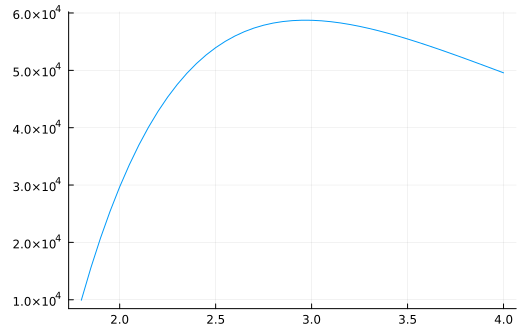
\includegraphics{./demand_estimation_2_files/figure-pdf/cell-23-output-1.svg}

}

\end{figure}

\begin{Shaded}
\begin{Highlighting}[]
\NormalTok{price\_range }\OperatorTok{=} \FunctionTok{range}\NormalTok{(}\FloatTok{1.8}\NormalTok{, }\FloatTok{4.0}\NormalTok{, step }\OperatorTok{=} \FloatTok{0.05}\NormalTok{);}
\NormalTok{totalpi\_res }\OperatorTok{=} \FunctionTok{f\_revenue}\NormalTok{.(}
\NormalTok{    price\_range, }
    \FunctionTok{Ref}\NormalTok{(data), }\FunctionTok{Ref}\NormalTok{(datalist), }\FunctionTok{Ref}\NormalTok{(parameter), }\FunctionTok{Ref}\NormalTok{(delta), }\FunctionTok{Ref}\NormalTok{(beta\_hat), }\FunctionTok{Ref}\NormalTok{(gmm\_res.minimizer),}
    \StringTok{"totalpi"}
\NormalTok{);}
\FunctionTok{plot}\NormalTok{(price\_range, totalpi\_res, legend }\OperatorTok{=} \ConstantTok{false}\NormalTok{)}
\end{Highlighting}
\end{Shaded}

\begin{figure}[H]

{\centering 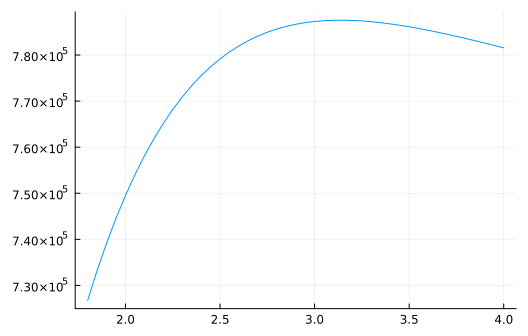
\includegraphics{./demand_estimation_2_files/figure-pdf/cell-24-output-1.svg}

}

\end{figure}

\begin{Shaded}
\begin{Highlighting}[]
\NormalTok{ownpi\_optim\_res }\OperatorTok{=} \FunctionTok{optimize}\NormalTok{(}
\NormalTok{    x }\OperatorTok{{-}\textgreater{}} \OperatorTok{{-}} \FunctionTok{f\_revenue}\NormalTok{(x[}\FloatTok{1}\NormalTok{], data, datalist, parameter, delta, beta\_hat, gmm\_res.minimizer, }\StringTok{"ownpi"}\NormalTok{),}
\NormalTok{    [}\FloatTok{3.0}\NormalTok{]}
\NormalTok{)}

\NormalTok{ownpi\_optim\_res.minimizer}
\end{Highlighting}
\end{Shaded}

\begin{verbatim}
1-element Vector{Float64}:
 2.967175245285034
\end{verbatim}

\begin{Shaded}
\begin{Highlighting}[]
\NormalTok{totalpi\_optim\_res }\OperatorTok{=} \FunctionTok{optimize}\NormalTok{(}
\NormalTok{    x }\OperatorTok{{-}\textgreater{}} \OperatorTok{{-}} \FunctionTok{f\_revenue}\NormalTok{(x[}\FloatTok{1}\NormalTok{], data, datalist, parameter, delta, beta\_hat, gmm\_res.minimizer, }\StringTok{"totalpi"}\NormalTok{),}
\NormalTok{    [}\FloatTok{3.0}\NormalTok{]}
\NormalTok{)}
\NormalTok{totalpi\_optim\_res.minimizer}
\end{Highlighting}
\end{Shaded}

\begin{verbatim}
1-element Vector{Float64}:
 3.136022758483887
\end{verbatim}

\bookmarksetup{startatroot}

\hypertarget{ux9700ux8981ux30e2ux30c7ux30ebux306eux63a8ux5b9aux5fdcux7528ux7de8}{%
\chapter{需要モデルの推定(応用編)}\label{ux9700ux8981ux30e2ux30c7ux30ebux306eux63a8ux5b9aux5fdcux7528ux7de8}}

\begin{Shaded}
\begin{Highlighting}[]
\ImportTok{using} \BuiltInTok{CSV}
\ImportTok{using} \BuiltInTok{DataFrames}
\ImportTok{using} \BuiltInTok{StringEncodings}
\ImportTok{using} \BuiltInTok{FixedEffectModels}
\ImportTok{using} \BuiltInTok{RegressionTables}
\ImportTok{using} \BuiltInTok{Plots}
\ImportTok{using} \BuiltInTok{LinearAlgebra}
\ImportTok{using} \BuiltInTok{Statistics}
\ImportTok{using} \BuiltInTok{Optim}
\ImportTok{using} \BuiltInTok{Printf}
\ImportTok{using} \BuiltInTok{ForwardDiff}
\ImportTok{using} \BuiltInTok{Random}
\ImportTok{using} \BuiltInTok{GLM}
\ImportTok{using} \BuiltInTok{Serialization}
\end{Highlighting}
\end{Shaded}

\begin{Shaded}
\begin{Highlighting}[]
\NormalTok{data }\OperatorTok{=}\NormalTok{ CSV.}\FunctionTok{read}\NormalTok{(}\StringTok{"data/demand\_estimation\_merger/chap3\_data.csv"}\NormalTok{, DataFrame);}
\FunctionTok{first}\NormalTok{(data, }\FloatTok{5}\NormalTok{)}
\end{Highlighting}
\end{Shaded}

\begin{tabular}{r|cccccccccc}
    & NameID & year & Maker & Type & Name & Sales & Model & price & kata & \\
    \hline
    & Int64 & Int64 & String15 & String7 & String31 & Int64 & String & Float64 & String15 & \\
    \hline
    1 & 14 & 2011 & Audi & Foreign & A1シリーズ & 4206 & 1.4 TFSI & 2.99804 & DBA-8XCAX & $\dots$ \\
    2 & 14 & 2012 & Audi & Foreign & A1シリーズ & 4502 & 1.4 TFSI & 2.835 & DBA-8XCAX & $\dots$ \\
    3 & 14 & 2013 & Audi & Foreign & A1シリーズ & 5071 & 1.4 TFSI & 2.82326 & DBA-8XCAX & $\dots$ \\
    4 & 15 & 2006 & Audi & Foreign & A3シリーズ & 4830 & アトラクション & 2.91889 & GH-8PBSE & $\dots$ \\
    5 & 15 & 2007 & Audi & Foreign & A3シリーズ & 3874 & アトラクション & 2.93944 & GH-8PBSE & $\dots$ \\
\end{tabular}

\begin{Shaded}
\begin{Highlighting}[]
\NormalTok{data[!, }\OperatorTok{:}\NormalTok{Foreign\_d] }\OperatorTok{=}\NormalTok{ data[}\OperatorTok{:}\NormalTok{, }\OperatorTok{:}\DataTypeTok{Type}\NormalTok{] }\OperatorTok{.==} \StringTok{"Foreign"}\NormalTok{;}
\NormalTok{data[!, }\OperatorTok{:}\NormalTok{FuelRegular\_d] }\OperatorTok{=}\NormalTok{ data[}\OperatorTok{:}\NormalTok{, }\OperatorTok{:}\NormalTok{FuelType] }\OperatorTok{.==} \StringTok{"レギュラー"}\NormalTok{;}
\NormalTok{data[!, }\OperatorTok{:}\NormalTok{capacity\_d] }\OperatorTok{=}\NormalTok{ data[}\OperatorTok{:}\NormalTok{, }\OperatorTok{:}\NormalTok{capacity] }\OperatorTok{.\textgreater{}} \FloatTok{4}\NormalTok{;}
\FunctionTok{transform!}\NormalTok{(data, [}\OperatorTok{:}\NormalTok{year }\OperatorTok{=\textgreater{}} \FunctionTok{ByRow}\NormalTok{(}\FunctionTok{isequal}\NormalTok{(v))}\OperatorTok{=\textgreater{}} \FunctionTok{Symbol}\NormalTok{(}\StringTok{"year\_"} \OperatorTok{*} \FunctionTok{string}\NormalTok{(v)) for v }\KeywordTok{in} \FunctionTok{unique}\NormalTok{(data.year)]);}
\FunctionTok{select!}\NormalTok{(data, }\FunctionTok{Not}\NormalTok{(}\OperatorTok{:}\NormalTok{year\_2006));}
\end{Highlighting}
\end{Shaded}

\hypertarget{section-7}{%
\section{4.2}\label{section-7}}

\begin{Shaded}
\begin{Highlighting}[]
\FunctionTok{sort!}\NormalTok{(data, [}\OperatorTok{:}\NormalTok{year, }\OperatorTok{:}\NormalTok{Maker, }\OperatorTok{:}\NormalTok{price]);}
\NormalTok{N }\OperatorTok{=} \FunctionTok{nrow}\NormalTok{(data);}
\NormalTok{T }\OperatorTok{=} \FunctionTok{length}\NormalTok{(}\FunctionTok{unique}\NormalTok{(data.year));}
\NormalTok{X1 }\OperatorTok{=} \FunctionTok{hcat}\NormalTok{(}
    \FunctionTok{repeat}\NormalTok{([}\FloatTok{1}\NormalTok{], N), }
    \FunctionTok{Matrix}\NormalTok{(data[}\OperatorTok{:}\NormalTok{, [}\OperatorTok{:}\NormalTok{price, }\OperatorTok{:}\NormalTok{FuelEfficiency, }\OperatorTok{:}\NormalTok{hppw, }\OperatorTok{:}\NormalTok{size, }\OperatorTok{:}\NormalTok{capacity\_d, }\OperatorTok{:}\NormalTok{FuelRegular\_d, }\OperatorTok{:}\NormalTok{Foreign\_d]]),}
    \FunctionTok{Matrix}\NormalTok{(data[}\OperatorTok{:}\NormalTok{, }\StringTok{r"\^{}year\_"}\NormalTok{])    }
\NormalTok{    );}
\NormalTok{X2 }\OperatorTok{=} \FunctionTok{Matrix}\NormalTok{(data[}\OperatorTok{:}\NormalTok{, [}\OperatorTok{:}\NormalTok{price]]);}
\NormalTok{Z }\OperatorTok{=} \FunctionTok{hcat}\NormalTok{(}
    \FunctionTok{repeat}\NormalTok{([}\FloatTok{1}\NormalTok{], N),}
    \FunctionTok{Matrix}\NormalTok{(data[}\OperatorTok{:}\NormalTok{, [}\OperatorTok{:}\NormalTok{FuelEfficiency, }\OperatorTok{:}\NormalTok{hppw, }\OperatorTok{:}\NormalTok{size, }\OperatorTok{:}\NormalTok{capacity\_d, }\OperatorTok{:}\NormalTok{FuelRegular\_d, }\OperatorTok{:}\NormalTok{Foreign\_d]]),}
    \FunctionTok{Matrix}\NormalTok{(data[}\OperatorTok{:}\NormalTok{, }\StringTok{r"\^{}year\_"}\NormalTok{]),}
    \FunctionTok{Matrix}\NormalTok{(data[}\OperatorTok{:}\NormalTok{, }\StringTok{r"\^{}iv\_GH}\SpecialCharTok{.*}\CharTok{(?}\StringTok{\textless{}!nest}\CharTok{)}\SpecialCharTok{$}\StringTok{"])}
\StringTok{    );}
\NormalTok{Random}\SpecialCharTok{.}\StringTok{seed!}\CharTok{(}\StringTok{42}\CharTok{)}\StringTok{;}
\NormalTok{Nsim }\OperatorTok{=} \FloatTok{1000}\NormalTok{;}

\NormalTok{draw\_vec }\OperatorTok{=} \FunctionTok{reduce}\NormalTok{(hcat, [}\FunctionTok{randn}\NormalTok{(}\FunctionTok{size}\NormalTok{(X2, }\FloatTok{2}\NormalTok{)) for j }\OperatorTok{=}\FloatTok{1}\OperatorTok{:}\NormalTok{Nsim]);}

\NormalTok{marketindex }\OperatorTok{=}\NormalTok{ data.year;}
\NormalTok{uniquemarketindex }\OperatorTok{=} \FunctionTok{sort}\NormalTok{(}\FunctionTok{unique}\NormalTok{(data.year));}
\end{Highlighting}
\end{Shaded}

\begin{Shaded}
\begin{Highlighting}[]
\NormalTok{temp1 }\OperatorTok{=} \FunctionTok{reduce}\NormalTok{(hcat, [uniquemarketindex for j }\OperatorTok{=} \FloatTok{1}\OperatorTok{:}\NormalTok{N])}\CharTok{\textquotesingle{};}
\NormalTok{temp2 }\OperatorTok{=} \FunctionTok{reduce}\NormalTok{(hcat, [data.year for j }\OperatorTok{=} \FloatTok{1}\OperatorTok{:}\NormalTok{T]);}
\NormalTok{mkt\_denom\_d }\OperatorTok{=}\NormalTok{ (temp1 }\OperatorTok{.==}\NormalTok{ temp2);}

\KeywordTok{mutable struct}\NormalTok{ datalist\_struct}
\NormalTok{    X1}\OperatorTok{::}\DataTypeTok{Array\{Float64,2\}}\NormalTok{;}
\NormalTok{    X2}\OperatorTok{::}\DataTypeTok{Array\{Float64,2\}}\NormalTok{;}
\NormalTok{    Z}\OperatorTok{::}\DataTypeTok{Array\{Float64,2\}}\NormalTok{;}
\NormalTok{    ShareVec}\OperatorTok{::}\DataTypeTok{Vector\{Float64\}}\NormalTok{;}
\NormalTok{    marketindex}\OperatorTok{::}\DataTypeTok{Vector\{Int64\}}\NormalTok{;}
\NormalTok{    logitshare}\OperatorTok{::}\DataTypeTok{Vector\{Float64\}}\NormalTok{;}
\NormalTok{    draw\_vec}\OperatorTok{::}\DataTypeTok{Array\{Float64,2\}}\NormalTok{;}
\NormalTok{    mkt\_denom\_d}\OperatorTok{::}\DataTypeTok{BitMatrix}
\KeywordTok{end}

\KeywordTok{mutable struct}\NormalTok{ parameter\_struct}
\NormalTok{    Nsim}\OperatorTok{::}\DataTypeTok{Int}\NormalTok{;}
\NormalTok{    T}\OperatorTok{::}\DataTypeTok{Int}\NormalTok{;}
\NormalTok{    N}\OperatorTok{::}\DataTypeTok{Int}\NormalTok{;}
\KeywordTok{end}
\NormalTok{datalist }\OperatorTok{=} \FunctionTok{datalist\_struct}\NormalTok{(X1, X2, Z, data.share, marketindex, data.logit\_share, draw\_vec, mkt\_denom\_d);}
\NormalTok{parameter }\OperatorTok{=} \FunctionTok{parameter\_struct}\NormalTok{(Nsim, T, N);}
\end{Highlighting}
\end{Shaded}

\hypertarget{section-8}{%
\section{4.3}\label{section-8}}

\begin{Shaded}
\begin{Highlighting}[]
\KeywordTok{function} \FunctionTok{f\_mktshare}\NormalTok{(}
\NormalTok{        theta2,}
\NormalTok{        datalist}\OperatorTok{::}\DataTypeTok{datalist\_struct}\NormalTok{,}
\NormalTok{        parameter}\OperatorTok{::}\DataTypeTok{parameter\_struct}\NormalTok{,}
\CommentTok{\#         delta::Vector\{Float64\}}
\NormalTok{        delta}
\NormalTok{    )}
        
\NormalTok{    mu }\OperatorTok{=}\NormalTok{ datalist.X2 }\OperatorTok{*} \FunctionTok{Diagonal}\NormalTok{(theta2) }\OperatorTok{*}\NormalTok{ datalist.draw\_vec;}
    
\NormalTok{    delta\_mu }\OperatorTok{=}\NormalTok{ delta }\OperatorTok{.*} \FunctionTok{ones}\NormalTok{((}\FloatTok{1}\NormalTok{, parameter.Nsim)) }\OperatorTok{.+}\NormalTok{ mu;}
\NormalTok{    exp\_delta\_mu }\OperatorTok{=} \FunctionTok{exp}\NormalTok{.(delta\_mu }\OperatorTok{.{-}} \FunctionTok{maximum}\NormalTok{(delta\_mu));}
\NormalTok{    denom\_outside }\OperatorTok{=} \FunctionTok{exp}\NormalTok{.(}\FunctionTok{{-}maximum}\NormalTok{(delta\_mu));}
    
\NormalTok{    denom\_temp }\OperatorTok{=}\NormalTok{ (exp\_delta\_mu}\OperatorTok{\textquotesingle{}} \OperatorTok{*}\NormalTok{ datalist.mkt\_denom\_d)}\CharTok{\textquotesingle{} .+ denom\_outside;}
\NormalTok{    denom }\OperatorTok{=}\NormalTok{ datalist.mkt\_denom\_d }\OperatorTok{*}\NormalTok{ denom\_temp;}
    
\NormalTok{    s\_jt\_i }\OperatorTok{=}\NormalTok{ exp\_delta\_mu }\OperatorTok{./}\NormalTok{ denom;}
\NormalTok{    s\_jt }\OperatorTok{=} \FunctionTok{vec}\NormalTok{(}\FunctionTok{mean}\NormalTok{(s\_jt\_i, dims }\OperatorTok{=} \FloatTok{2}\NormalTok{));}
    
    \ControlFlowTok{return}\NormalTok{ s\_jt}
    
\KeywordTok{end}
\end{Highlighting}
\end{Shaded}

\begin{verbatim}
f_mktshare (generic function with 1 method)
\end{verbatim}

\begin{Shaded}
\begin{Highlighting}[]
\KeywordTok{function} \FunctionTok{f\_contraction}\NormalTok{(}
\NormalTok{        theta2,}
\NormalTok{        datalist}\OperatorTok{::}\DataTypeTok{datalist\_struct}\NormalTok{,}
\NormalTok{        parameter}\OperatorTok{::}\DataTypeTok{parameter\_struct}\NormalTok{,}
\NormalTok{        delta\_ini}\OperatorTok{::}\DataTypeTok{Vector\{Float64\}}
\NormalTok{    )}
    
\NormalTok{    tol }\OperatorTok{=} \FloatTok{1e{-}11}\NormalTok{;}
\NormalTok{    norm }\OperatorTok{=} \FloatTok{1e+10}

\NormalTok{    delta\_old }\OperatorTok{=}\NormalTok{ delta\_ini;}
\NormalTok{    exp\_delta\_old }\OperatorTok{=} \FunctionTok{exp}\NormalTok{.(delta\_old);}
    
\NormalTok{    iter }\OperatorTok{=} \FloatTok{0}\NormalTok{;}
        
    \ControlFlowTok{while}\NormalTok{ ((norm }\OperatorTok{\textgreater{}}\NormalTok{ tol) }\OperatorTok{\&}\NormalTok{ (iter }\OperatorTok{\textless{}} \FloatTok{1000}\NormalTok{))}
        
        \CommentTok{\# print(iter, "\textbackslash{}n")}
        
\NormalTok{        pred\_mkt\_share }\OperatorTok{=} \FunctionTok{f\_mktshare}\NormalTok{(theta2, datalist, parameter, delta\_old);}
        
\NormalTok{        exp\_delta }\OperatorTok{=}\NormalTok{ exp\_delta\_old }\OperatorTok{.*}\NormalTok{ datalist.ShareVec }\OperatorTok{./}\NormalTok{ pred\_mkt\_share;}
        
\NormalTok{        norm }\OperatorTok{=} \FunctionTok{maximum}\NormalTok{(}\FunctionTok{abs}\NormalTok{.(exp\_delta }\OperatorTok{.{-}}\NormalTok{ exp\_delta\_old));}
        
\NormalTok{        exp\_delta\_old }\OperatorTok{=}\NormalTok{ exp\_delta;}
\NormalTok{        delta\_old }\OperatorTok{=} \FunctionTok{log}\NormalTok{.(exp\_delta\_old);}
\NormalTok{        iter }\OperatorTok{+=} \FloatTok{1}\NormalTok{;}
        
    \ControlFlowTok{end}
    
\CommentTok{\#     print(iter, "\textbackslash{}n")}
    
    \ControlFlowTok{return}\NormalTok{ delta\_old;}
    
\KeywordTok{end}
\end{Highlighting}
\end{Shaded}

\begin{verbatim}
f_contraction (generic function with 1 method)
\end{verbatim}

\begin{Shaded}
\begin{Highlighting}[]
\KeywordTok{function} \FunctionTok{f\_GMMobj}\NormalTok{(}
\NormalTok{        theta2,}
\NormalTok{        parameter}\OperatorTok{::}\DataTypeTok{parameter\_struct}\NormalTok{,}
\NormalTok{        datalist}\OperatorTok{::}\DataTypeTok{datalist\_struct}\NormalTok{,}
\NormalTok{        delta\_ini}\OperatorTok{::}\DataTypeTok{Vector\{Float64\}}
\NormalTok{    )}
    
\CommentTok{\#     delta\_ini = delta\_global;}
\CommentTok{\#     delta\_ini = datalist.logitshare;}
\NormalTok{    delta }\OperatorTok{=} \FunctionTok{f\_contraction}\NormalTok{(theta2, datalist, parameter, delta\_ini);}
\CommentTok{\#     global delta\_global = delta}
    
\CommentTok{\#     if (datalist.weight\_mat\_option == "2SLS") }
\NormalTok{        W }\OperatorTok{=} \FunctionTok{inv}\NormalTok{(datalist.Z}\OperatorTok{\textquotesingle{}} \OperatorTok{*}\NormalTok{ datalist.Z);}
\CommentTok{\#     elseif (datalist.weight\_mat\_option == "Ident")}
\CommentTok{\#         W = I(size(datalist.Z, 2));}
\CommentTok{\#     end}
    
\NormalTok{    beta\_hat }\OperatorTok{=}\NormalTok{ (datalist.X1}\OperatorTok{\textquotesingle{}} \OperatorTok{*}\NormalTok{ datalist.Z }\OperatorTok{*}\NormalTok{ W }\OperatorTok{*}\NormalTok{ datalist.Z}\OperatorTok{\textquotesingle{}} \OperatorTok{*}\NormalTok{ datalist.X1) }\OperatorTok{\textbackslash{}}\NormalTok{ (datalist.X1}\OperatorTok{\textquotesingle{}} \OperatorTok{*}\NormalTok{ datalist.Z }\OperatorTok{*}\NormalTok{ W }\OperatorTok{*}\NormalTok{ datalist.Z}\OperatorTok{\textquotesingle{}} \OperatorTok{*}\NormalTok{ delta);}
    
\NormalTok{    Xi }\OperatorTok{=}\NormalTok{ delta }\OperatorTok{{-}}\NormalTok{ datalist.X1 }\OperatorTok{*}\NormalTok{ beta\_hat;}
    
\NormalTok{    output }\OperatorTok{=}\NormalTok{ Xi}\OperatorTok{\textquotesingle{}} \OperatorTok{*}\NormalTok{ datalist.Z }\OperatorTok{*}\NormalTok{ W }\OperatorTok{*}\NormalTok{ datalist.Z}\OperatorTok{\textquotesingle{}} \OperatorTok{*}\NormalTok{ Xi}
        
    \ControlFlowTok{return}\NormalTok{ output}
    
\KeywordTok{end}    
\end{Highlighting}
\end{Shaded}

\begin{verbatim}
f_GMMobj (generic function with 1 method)
\end{verbatim}

\begin{Shaded}
\begin{Highlighting}[]
\NormalTok{initial\_x }\OperatorTok{=}\NormalTok{ [}\FloatTok{0.1}\NormalTok{];}
\NormalTok{delta\_ini }\OperatorTok{=} \FunctionTok{f\_contraction}\NormalTok{(initial\_x, datalist, parameter, datalist.logitshare);}
\NormalTok{objFunc\_for\_Optim }\OperatorTok{=} \FunctionTok{TwiceDifferentiable}\NormalTok{(}
\NormalTok{    x }\OperatorTok{{-}\textgreater{}} \FunctionTok{f\_GMMobj}\NormalTok{(x, parameter, datalist, delta\_ini),}
\NormalTok{    initial\_x;}
\NormalTok{    autodiff }\OperatorTok{=} \OperatorTok{:}\NormalTok{forward}
\NormalTok{    );}
\end{Highlighting}
\end{Shaded}

\begin{Shaded}
\begin{Highlighting}[]
\PreprocessorTok{@time}\NormalTok{ gmm\_res }\OperatorTok{=} \FunctionTok{optimize}\NormalTok{(}
\NormalTok{    objFunc\_for\_Optim,}
\CommentTok{\#     x {-}\textgreater{} f\_GMMobj(x, parameter, datalist, delta\_ini),}
\NormalTok{    [}\FloatTok{0.0}\NormalTok{],}
\NormalTok{    [}\ConstantTok{Inf}\NormalTok{],}
\NormalTok{    initial\_x,}
\NormalTok{    Optim.}\FunctionTok{Options}\NormalTok{(show\_trace }\OperatorTok{=} \ConstantTok{true}\NormalTok{)}
\NormalTok{)}
\end{Highlighting}
\end{Shaded}

\begin{Shaded}
\begin{Highlighting}[]
\NormalTok{W }\OperatorTok{=} \FunctionTok{inv}\NormalTok{(datalist.Z}\OperatorTok{\textquotesingle{}} \OperatorTok{*}\NormalTok{ datalist.Z);    }
\NormalTok{delta }\OperatorTok{=} \FunctionTok{f\_contraction}\NormalTok{(gmm\_res.minimizer, datalist, parameter, delta\_ini);}
\NormalTok{beta\_hat }\OperatorTok{=}\NormalTok{ (datalist.X1}\OperatorTok{\textquotesingle{}} \OperatorTok{*}\NormalTok{ datalist.Z }\OperatorTok{*}\NormalTok{ W }\OperatorTok{*}\NormalTok{ datalist.Z}\OperatorTok{\textquotesingle{}} \OperatorTok{*}\NormalTok{ datalist.X1) }\OperatorTok{\textbackslash{}}\NormalTok{ (datalist.X1}\OperatorTok{\textquotesingle{}} \OperatorTok{*}\NormalTok{ datalist.Z }\OperatorTok{*}\NormalTok{ W }\OperatorTok{*}\NormalTok{ datalist.Z}\OperatorTok{\textquotesingle{}} \OperatorTok{*}\NormalTok{ delta);}
\end{Highlighting}
\end{Shaded}

\begin{Shaded}
\begin{Highlighting}[]
\NormalTok{Xi }\OperatorTok{=}\NormalTok{ delta }\OperatorTok{{-}}\NormalTok{ X1 }\OperatorTok{*}\NormalTok{ beta\_hat;}
\NormalTok{Omega\_hat }\OperatorTok{=} \FunctionTok{reduce}\NormalTok{(}\OperatorTok{+}\NormalTok{, Z[i,}\OperatorTok{:}\NormalTok{] }\OperatorTok{*}\NormalTok{ Z[i,}\OperatorTok{:}\NormalTok{]}\CharTok{\textquotesingle{} .* Xi[i]\^{}2 ./ N for i = 1:N);}
\NormalTok{Ddelta }\OperatorTok{=}\NormalTok{ ForwardDiff.}\FunctionTok{jacobian}\NormalTok{(x }\OperatorTok{{-}\textgreater{}}\NormalTok{ delta\_ini }\OperatorTok{=} \FunctionTok{f\_contraction}\NormalTok{(x, datalist, parameter, delta), gmm\_res.minimizer);}
\NormalTok{G }\OperatorTok{=}\NormalTok{ Z}\OperatorTok{\textquotesingle{}} \OperatorTok{*} \FunctionTok{hcat}\NormalTok{(}\OperatorTok{{-}}\NormalTok{ X1, Ddelta) }\OperatorTok{./}\NormalTok{ N;}
\NormalTok{AsyVarMat }\OperatorTok{=}\NormalTok{ (G}\OperatorTok{\textquotesingle{}} \OperatorTok{*}\NormalTok{ W }\OperatorTok{*}\NormalTok{ G) }\OperatorTok{\textbackslash{}}\NormalTok{ G}\OperatorTok{\textquotesingle{}} \OperatorTok{*}\NormalTok{ W }\OperatorTok{*}\NormalTok{ Omega\_hat }\OperatorTok{*}\NormalTok{ W }\OperatorTok{*}\NormalTok{ G }\OperatorTok{*} \FunctionTok{inv}\NormalTok{(G}\OperatorTok{\textquotesingle{}} \OperatorTok{*}\NormalTok{ W }\OperatorTok{*}\NormalTok{ G);}
\NormalTok{Ase }\OperatorTok{=} \FunctionTok{sqrt}\NormalTok{.(}\FunctionTok{diag}\NormalTok{(AsyVarMat) }\OperatorTok{./}\NormalTok{ N);}
\FunctionTok{DataFrame}\NormalTok{(}
\NormalTok{    Var }\OperatorTok{=}\NormalTok{ [}
        \StringTok{"Const"}\NormalTok{, }\StringTok{"Price"}\NormalTok{, }\StringTok{"Fuel Efficiency"}\NormalTok{, }\StringTok{"hppw"}\NormalTok{, }\StringTok{"size"}\NormalTok{, }
        \StringTok{"capacity\_d"}\NormalTok{, }\StringTok{"FuelRegular\_d"}\NormalTok{, }\StringTok{"Foreign\_d"}\NormalTok{,}
        \StringTok{"year\_2007"}\NormalTok{, }\StringTok{"year\_2008"}\NormalTok{, }\StringTok{"year\_2009"}\NormalTok{, }
        \StringTok{"year\_2010"}\NormalTok{, }\StringTok{"year\_2011"}\NormalTok{, }\StringTok{"year\_2012"}\NormalTok{, }
        \StringTok{"year\_2013"}\NormalTok{, }\StringTok{"year\_2014"}\NormalTok{, }\StringTok{"year\_2015"}\NormalTok{, }\StringTok{"year\_2016"}\NormalTok{, }
        \StringTok{"random\_price"}
\NormalTok{        ],}
\NormalTok{    Est }\OperatorTok{=} \FunctionTok{vcat}\NormalTok{(beta\_hat, gmm\_res.minimizer),}
\NormalTok{    se }\OperatorTok{=}\NormalTok{ Ase}
\NormalTok{)}
\end{Highlighting}
\end{Shaded}

\begin{tabular}{r|ccc}
    & Var & Est & se\\
    \hline
    & String & Float64 & Float64\\
    \hline
    1 & Const & -13.8731 & 0.57026 \\
    2 & Price & -2.26772 & 0.654208 \\
    3 & Fuel Efficiency & 0.195358 & 0.0125426 \\
    4 & hppw & 14.123 & 3.47038 \\
    5 & size & 0.545374 & 0.0755396 \\
    6 & capacity\_d & -0.313033 & 0.137174 \\
    7 & FuelRegular\_d & -1.09267 & 0.283308 \\
    8 & Foreign\_d & 1.02095 & 0.188846 \\
    9 & year\_2007 & -0.832913 & 0.173999 \\
    10 & year\_2008 & -0.701377 & 0.167621 \\
    11 & year\_2009 & -0.85305 & 0.168625 \\
    12 & year\_2010 & -0.0979013 & 0.15156 \\
    13 & year\_2011 & -0.251012 & 0.150935 \\
    14 & year\_2012 & -0.482276 & 0.159593 \\
    15 & year\_2013 & -0.623362 & 0.165287 \\
    16 & year\_2014 & -1.04477 & 0.180093 \\
    17 & year\_2015 & -1.1434 & 0.178264 \\
    18 & year\_2016 & -1.24577 & 0.181075 \\
    19 & random\_price & 0.647326 & 0.218627 \\
\end{tabular}

\begin{Shaded}
\begin{Highlighting}[]
\NormalTok{mu }\OperatorTok{=}\NormalTok{ X2 }\OperatorTok{*} \FunctionTok{Diagonal}\NormalTok{(gmm\_res.minimizer) }\OperatorTok{*}\NormalTok{ draw\_vec;}
\NormalTok{delta\_mu }\OperatorTok{=}\NormalTok{ delta }\OperatorTok{.+}\NormalTok{ mu;}
\NormalTok{exp\_delta\_mu }\OperatorTok{=} \FunctionTok{exp}\NormalTok{.(delta\_mu);}
\NormalTok{denom\_outside }\OperatorTok{=} \FunctionTok{exp}\NormalTok{.(}\FloatTok{0.0}\NormalTok{);}
\NormalTok{denom\_temp }\OperatorTok{=}\NormalTok{ (exp\_delta\_mu}\OperatorTok{\textquotesingle{}} \OperatorTok{*}\NormalTok{ mkt\_denom\_d)}\CharTok{\textquotesingle{} .+ denom\_outside;}
\NormalTok{denom }\OperatorTok{=}\NormalTok{ mkt\_denom\_d }\OperatorTok{*}\NormalTok{ denom\_temp;}

\NormalTok{s\_jt\_i }\OperatorTok{=}\NormalTok{ exp\_delta\_mu }\OperatorTok{./}\NormalTok{ denom;}
\NormalTok{draw\_for\_price }\OperatorTok{=}\NormalTok{ draw\_vec[}\FloatTok{1}\NormalTok{,}\OperatorTok{:}\NormalTok{];}
\NormalTok{alpha\_i }\OperatorTok{=}\NormalTok{ beta\_hat[}\FloatTok{2}\NormalTok{] }\OperatorTok{.+}\NormalTok{ gmm\_res.minimizer[}\FloatTok{1}\NormalTok{] }\OperatorTok{.*}\NormalTok{ draw\_for\_price;}
\NormalTok{year }\OperatorTok{=} \FloatTok{2016}
\NormalTok{J\_t }\OperatorTok{=} \FunctionTok{sum}\NormalTok{(data.year }\OperatorTok{.==}\NormalTok{ year);}
\NormalTok{data\_t }\OperatorTok{=}\NormalTok{ data[data.year }\OperatorTok{.==}\NormalTok{ year, }\OperatorTok{:}\NormalTok{];}

\NormalTok{ag\_model\_s\_i }\OperatorTok{=}\NormalTok{ s\_jt\_i[data.year }\OperatorTok{.==}\NormalTok{ year, }\OperatorTok{:}\NormalTok{]}
\NormalTok{ag\_model\_s }\OperatorTok{=} \FunctionTok{mean}\NormalTok{(ag\_model\_s\_i, dims }\OperatorTok{=} \FloatTok{2}\NormalTok{);}
\NormalTok{price\_t }\OperatorTok{=}\NormalTok{ data.price[data.year }\OperatorTok{.==}\NormalTok{ year];}

\NormalTok{elasmat\_t }\OperatorTok{=} \FunctionTok{zeros}\NormalTok{((J\_t, J\_t));}

\ControlFlowTok{for}\NormalTok{ k }\KeywordTok{in} \FloatTok{1}\OperatorTok{:}\NormalTok{J\_t, j }\KeywordTok{in} \FloatTok{1}\OperatorTok{:}\NormalTok{J\_t}
    \ControlFlowTok{if}\NormalTok{ (k }\OperatorTok{!=}\NormalTok{ j)}
\NormalTok{        elasmat\_t[k, j] }\OperatorTok{=}\NormalTok{ (}\OperatorTok{{-}}\FloatTok{1.0}\NormalTok{) }\OperatorTok{.*}\NormalTok{ price\_t[k] }\OperatorTok{./}\NormalTok{ ag\_model\_s[j] }\OperatorTok{*} \FunctionTok{mean}\NormalTok{(alpha\_i }\OperatorTok{.*}\NormalTok{ ag\_model\_s\_i[j, }\OperatorTok{:}\NormalTok{] }\OperatorTok{.*}\NormalTok{ ag\_model\_s\_i[k, }\OperatorTok{:}\NormalTok{])}
    \ControlFlowTok{elseif}\NormalTok{ (k }\OperatorTok{==}\NormalTok{ j)}
\NormalTok{        elasmat\_t[k, j] }\OperatorTok{=}\NormalTok{ price\_t[j] }\OperatorTok{./}\NormalTok{ ag\_model\_s[j] }\OperatorTok{*} \FunctionTok{mean}\NormalTok{(alpha\_i }\OperatorTok{.*}\NormalTok{ ag\_model\_s\_i[j, }\OperatorTok{:}\NormalTok{] }\OperatorTok{.*}\NormalTok{ (}\FloatTok{1.0} \OperatorTok{.{-}}\NormalTok{ ag\_model\_s\_i[j, }\OperatorTok{:}\NormalTok{]))}
    \ControlFlowTok{end}
\ControlFlowTok{end}
\end{Highlighting}
\end{Shaded}

\hypertarget{section-9}{%
\section{5}\label{section-9}}

\begin{Shaded}
\begin{Highlighting}[]
\NormalTok{Pricevec\_t }\OperatorTok{=}\NormalTok{ data\_t.price;}
\NormalTok{Sharevec\_t }\OperatorTok{=}\NormalTok{ data\_t.share;}

\NormalTok{Ownership\_t }\OperatorTok{=}\NormalTok{ data\_t.Maker }\OperatorTok{.==} \FunctionTok{permutedims}\NormalTok{(data\_t.Maker);}
\NormalTok{Derivative\_t }\OperatorTok{=} \OperatorTok{{-}}\NormalTok{ elasmat\_t }\OperatorTok{.*}\NormalTok{ Sharevec\_t}\OperatorTok{\textquotesingle{}} \OperatorTok{./}\NormalTok{ Pricevec\_t;}
\NormalTok{Delta\_t }\OperatorTok{=}\NormalTok{ Derivative\_t }\OperatorTok{.*}\NormalTok{ Ownership\_t;}
\NormalTok{Marginal\_Cost\_t }\OperatorTok{=}\NormalTok{ Pricevec\_t }\OperatorTok{{-}}\NormalTok{ (Delta\_t }\OperatorTok{\textbackslash{}}\NormalTok{ Sharevec\_t);}
\NormalTok{pred\_mc\_df }\OperatorTok{=} \FunctionTok{DataFrame}\NormalTok{(}
\NormalTok{    Maker }\OperatorTok{=}\NormalTok{ data\_t.Maker, }
\NormalTok{    Name }\OperatorTok{=}\NormalTok{ data\_t.Name, }
\NormalTok{    Price }\OperatorTok{=}\NormalTok{ data\_t.price,}
\NormalTok{    MC }\OperatorTok{=} \FunctionTok{Vector}\DataTypeTok{\{Float64\}}\NormalTok{(Marginal\_Cost\_t),}
\NormalTok{    Margin }\OperatorTok{=}\NormalTok{ (data\_t.price }\OperatorTok{.{-}}\NormalTok{ Marginal\_Cost\_t) }\OperatorTok{./}\NormalTok{ data\_t.price}
\NormalTok{)}
\end{Highlighting}
\end{Shaded}

\begin{tabular}{r|ccccc}
    & Maker & Name & Price & MC & Margin\\
    \hline
    & String15 & String31 & Float64 & Float64 & Float64\\
    \hline
    1 & Audi & A3シリーズ & 3.28 & 2.37501 & 0.275912 \\
    2 & Audi & A4シリーズ & 5.18 & 3.63239 & 0.298766 \\
    3 & BMW & ミニ & 2.4 & 1.68184 & 0.299235 \\
    4 & BMW & 1シリーズ & 3.1 & 2.23582 & 0.278768 \\
    5 & BMW & X1 & 3.67 & 2.65528 & 0.276489 \\
    6 & BMW & 2シリーズ & 3.81 & 2.75368 & 0.27725 \\
    7 & BMW & 3シリーズ & 4.49 & 3.2058 & 0.286013 \\
    8 & Daihatsu & ミラ & 0.885 & 0.367591 & 0.584643 \\
    9 & Daihatsu & ムーヴ & 1.134 & 0.590801 & 0.479012 \\
    10 & Daihatsu & ブーン & 1.15 & 0.605056 & 0.473864 \\
    11 & Daihatsu & キャスト & 1.22 & 0.667293 & 0.453039 \\
    12 & Daihatsu & タント & 1.22 & 0.667293 & 0.453039 \\
    13 & Daihatsu & ウェイク & 1.35 & 0.782294 & 0.420523 \\
    14 & Daihatsu & アトレーワゴン & 1.404 & 0.829833 & 0.408951 \\
    15 & Daihatsu & トール & 1.463 & 0.881614 & 0.397393 \\
    16 & Daihatsu & ビーゴ & 1.738 & 1.12062 & 0.355223 \\
    17 & Daihatsu & コペン & 1.852 & 1.2185 & 0.342064 \\
    18 & Daihatsu & メビウス & 2.571 & 1.8168 & 0.29335 \\
    19 & Daihatsu & アルティス & 2.745 & 1.956 & 0.28743 \\
    20 & Fiat & 500 & 1.998 & 1.34902 & 0.324817 \\
    21 & Honda & N-WGN & 1.164 & 0.613683 & 0.472781 \\
    22 & Honda & N-ONE & 1.185 & 0.632313 & 0.466402 \\
    23 & Honda & N-BOX & 1.27 & 0.707519 & 0.442898 \\
    24 & Honda & フィット & 1.3 & 0.733983 & 0.435398 \\
    25 & Honda & バモス & 1.374 & 0.799078 & 0.418429 \\
    26 & Honda & シャトル & 1.695 & 1.07825 & 0.363862 \\
    27 & Honda & グレイス & 1.75 & 1.12553 & 0.356839 \\
    28 & Honda & フリード & 1.88 & 1.23659 & 0.342242 \\
    29 & Honda & ヴェゼル & 1.92 & 1.27055 & 0.338254 \\
    30 & Honda & S660 & 1.98 & 1.32132 & 0.332666 \\
    $\dots$ & $\dots$ & $\dots$ & $\dots$ & $\dots$ & $\dots$ \\
\end{tabular}

\begin{Shaded}
\begin{Highlighting}[]
\FunctionTok{histogram}\NormalTok{(pred\_mc\_df.Margin, bins }\OperatorTok{=} \FloatTok{40}\NormalTok{, legend }\OperatorTok{=} \ConstantTok{false}\NormalTok{)}
\end{Highlighting}
\end{Shaded}

\begin{figure}[H]

{\centering 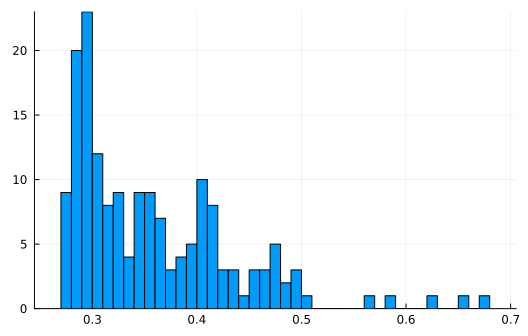
\includegraphics{./demand_estimation_merger_files/figure-pdf/cell-20-output-1.svg}

}

\end{figure}

\hypertarget{section-10}{%
\section{6}\label{section-10}}

\begin{Shaded}
\begin{Highlighting}[]
\NormalTok{data\_2016 }\OperatorTok{=}\NormalTok{ data[data.year }\OperatorTok{.==} \FloatTok{2016}\NormalTok{, }\OperatorTok{:}\NormalTok{];}
\NormalTok{data\_2016 }\OperatorTok{=} \FunctionTok{leftjoin}\NormalTok{(data\_2016, pred\_mc\_df, on }\OperatorTok{=}\NormalTok{ [}\StringTok{"Maker"}\NormalTok{, }\StringTok{"Name"}\NormalTok{]);}
\FunctionTok{dropmissing!}\NormalTok{(data\_2016);}

\NormalTok{data\_2016[data\_2016.Maker }\OperatorTok{.==} \StringTok{"Honda"}\NormalTok{, }\OperatorTok{:}\NormalTok{Maker] }\OperatorTok{.=} \StringTok{"Nippyo"}\NormalTok{;}
\NormalTok{data\_2016[data\_2016.Maker }\OperatorTok{.==} \StringTok{"Nissan"}\NormalTok{, }\OperatorTok{:}\NormalTok{Maker] }\OperatorTok{.=} \StringTok{"BrandA"}\NormalTok{;}
\NormalTok{data\_2016[data\_2016.Maker }\OperatorTok{.==} \StringTok{"Subaru"}\NormalTok{, }\OperatorTok{:}\NormalTok{Maker] }\OperatorTok{.=} \StringTok{"BrandB"}\NormalTok{;}
\NormalTok{data\_2016[data\_2016.Maker }\OperatorTok{.==} \StringTok{"Toyota"}\NormalTok{, }\OperatorTok{:}\NormalTok{Maker] }\OperatorTok{.=} \StringTok{"BrandC"}\NormalTok{;}

\NormalTok{data\_2016[!, }\OperatorTok{:}\NormalTok{MakerNippyoA] }\OperatorTok{=}\NormalTok{ data\_2016[}\OperatorTok{:}\NormalTok{, }\OperatorTok{:}\NormalTok{Maker];}
\NormalTok{data\_2016[!, }\OperatorTok{:}\NormalTok{MakerNippyoB] }\OperatorTok{=}\NormalTok{ data\_2016[}\OperatorTok{:}\NormalTok{, }\OperatorTok{:}\NormalTok{Maker];}
\NormalTok{data\_2016[}\FunctionTok{in}\NormalTok{([}\StringTok{"Nippyo"}\NormalTok{, }\StringTok{"BrandA"}\NormalTok{]).(data\_2016[}\OperatorTok{:}\NormalTok{, }\OperatorTok{:}\NormalTok{Maker]), }\OperatorTok{:}\NormalTok{MakerNippyoA] }\OperatorTok{.=} \StringTok{"NippyoA"}\NormalTok{;}
\NormalTok{data\_2016[}\FunctionTok{in}\NormalTok{([}\StringTok{"Nippyo"}\NormalTok{, }\StringTok{"BrandB"}\NormalTok{]).(data\_2016[}\OperatorTok{:}\NormalTok{, }\OperatorTok{:}\NormalTok{Maker]), }\OperatorTok{:}\NormalTok{MakerNippyoB] }\OperatorTok{.=} \StringTok{"NippyoB"}\NormalTok{;}
\NormalTok{J }\OperatorTok{=} \FunctionTok{nrow}\NormalTok{(data\_2016);}

\NormalTok{Ownership\_true }\OperatorTok{=}\NormalTok{ data\_2016.Maker }\OperatorTok{.==} \FunctionTok{permutedims}\NormalTok{(data\_2016.Maker);}
\NormalTok{Ownership\_NippyoA }\OperatorTok{=}\NormalTok{ data\_2016.MakerNippyoA }\OperatorTok{.==} \FunctionTok{permutedims}\NormalTok{(data\_2016.MakerNippyoA);}
\NormalTok{Ownership\_NippyoB }\OperatorTok{=}\NormalTok{ data\_2016.MakerNippyoB }\OperatorTok{.==} \FunctionTok{permutedims}\NormalTok{(data\_2016.MakerNippyoB);}
\end{Highlighting}
\end{Shaded}

\hypertarget{section-11}{%
\section{6.4}\label{section-11}}

\begin{Shaded}
\begin{Highlighting}[]
\NormalTok{mc }\OperatorTok{=}\NormalTok{ data\_2016.MC;}
\NormalTok{datalist\_2016 }\OperatorTok{=} \FunctionTok{datalist\_struct}\NormalTok{(}
\NormalTok{    X1[data.year }\OperatorTok{.==} \FloatTok{2016}\NormalTok{, }\OperatorTok{:}\NormalTok{],}
\NormalTok{    X2[data.year }\OperatorTok{.==} \FloatTok{2016}\NormalTok{, }\OperatorTok{:}\NormalTok{],}
\NormalTok{    Z[data.year }\OperatorTok{.==} \FloatTok{2016}\NormalTok{, }\OperatorTok{:}\NormalTok{],}
\NormalTok{    data\_2016.share,}
\NormalTok{    data\_2016.year,}
\NormalTok{    data\_2016.logit\_share,}
\NormalTok{    datalist.draw\_vec,}
\NormalTok{    datalist.mkt\_denom\_d[data.year }\OperatorTok{.==} \FloatTok{2016}\NormalTok{, }\OperatorTok{:}\NormalTok{]}
\NormalTok{);}
\end{Highlighting}
\end{Shaded}

\begin{Shaded}
\begin{Highlighting}[]
\KeywordTok{function} \FunctionTok{f\_update}\NormalTok{(}
\NormalTok{        datalist}\OperatorTok{::}\DataTypeTok{datalist\_struct}\NormalTok{,}
\NormalTok{        p\_old}\OperatorTok{::}\DataTypeTok{Vector\{Float64\}}\NormalTok{,}
\NormalTok{        Ownership}\OperatorTok{::}\DataTypeTok{BitMatrix}\NormalTok{,}
\NormalTok{        parameter}\OperatorTok{::}\DataTypeTok{parameter\_struct}\NormalTok{,}
\NormalTok{        theta1}\OperatorTok{::}\DataTypeTok{Vector\{Float64\}}\NormalTok{,}
\NormalTok{        theta2}\OperatorTok{::}\DataTypeTok{Vector\{Float64\}}\NormalTok{,}
\NormalTok{        mc}\OperatorTok{::}\DataTypeTok{Vector\{Float64\}}\NormalTok{,}
\NormalTok{        Xi}\OperatorTok{::}\DataTypeTok{Vector\{Float64\}}
\NormalTok{    )}
    
\NormalTok{    X1\_new }\OperatorTok{=}\NormalTok{ datalist.X1[}\OperatorTok{:}\NormalTok{, }\OperatorTok{:}\NormalTok{];}
\NormalTok{    X2\_new }\OperatorTok{=} \FunctionTok{reshape}\NormalTok{(p\_old, (}\OperatorTok{:}\NormalTok{, }\FloatTok{1}\NormalTok{));}
\NormalTok{    X1\_new[}\OperatorTok{:}\NormalTok{, }\FloatTok{2}\NormalTok{] }\OperatorTok{.=}\NormalTok{ p\_old;}
    
\NormalTok{    delta }\OperatorTok{=}\NormalTok{ (X1\_new }\OperatorTok{*}\NormalTok{ theta1) }\OperatorTok{.+}\NormalTok{ Xi;}
\NormalTok{    datalist\_new }\OperatorTok{=} \FunctionTok{datalist\_struct}\NormalTok{(}
\NormalTok{        X1\_new, X2\_new, datalist.Z, datalist.ShareVec, datalist.marketindex, }
\NormalTok{        datalist.logitshare, datalist.draw\_vec, datalist.mkt\_denom\_d}
\NormalTok{        );}
\NormalTok{    Sharevec }\OperatorTok{=} \FunctionTok{f\_mktshare}\NormalTok{(}
\NormalTok{        theta2, datalist\_new, parameter, delta}
\NormalTok{    );}
    
    \CommentTok{\# elasticity}
\NormalTok{    mu }\OperatorTok{=}\NormalTok{ datalist\_new.X2 }\OperatorTok{*} \FunctionTok{Diagonal}\NormalTok{(theta2) }\OperatorTok{*}\NormalTok{ datalist\_new.draw\_vec;}
\NormalTok{    delta\_mu }\OperatorTok{=}\NormalTok{ delta }\OperatorTok{.+}\NormalTok{ mu;}
\NormalTok{    exp\_delta\_mu }\OperatorTok{=} \FunctionTok{exp}\NormalTok{.(delta\_mu);}
\NormalTok{    denom\_outside }\OperatorTok{=} \FunctionTok{exp}\NormalTok{.(}\FloatTok{0.0}\NormalTok{);}
\NormalTok{    denom\_temp }\OperatorTok{=}\NormalTok{ (exp\_delta\_mu}\OperatorTok{\textquotesingle{}} \OperatorTok{*}\NormalTok{ datalist\_new.mkt\_denom\_d)}\CharTok{\textquotesingle{} .+ denom\_outside;}
\NormalTok{    denom }\OperatorTok{=}\NormalTok{ datalist\_new.mkt\_denom\_d }\OperatorTok{*}\NormalTok{ denom\_temp;}

\NormalTok{    s\_jt\_i }\OperatorTok{=}\NormalTok{ exp\_delta\_mu }\OperatorTok{./}\NormalTok{ denom;}
\NormalTok{    draw\_for\_price }\OperatorTok{=}\NormalTok{ datalist\_new.draw\_vec[}\FloatTok{1}\NormalTok{,}\OperatorTok{:}\NormalTok{];}
\NormalTok{    alpha\_i }\OperatorTok{=}\NormalTok{ theta1[}\FloatTok{2}\NormalTok{] }\OperatorTok{.+}\NormalTok{ theta2[}\FloatTok{1}\NormalTok{] }\OperatorTok{.*}\NormalTok{ draw\_for\_price;}
    
\NormalTok{    J }\OperatorTok{=} \FunctionTok{size}\NormalTok{(X1\_new, }\FloatTok{1}\NormalTok{);}
    
\NormalTok{    ag\_model\_s }\OperatorTok{=} \FunctionTok{mean}\NormalTok{(s\_jt\_i, dims }\OperatorTok{=} \FloatTok{2}\NormalTok{);}
\NormalTok{    elasmat }\OperatorTok{=} \FunctionTok{zeros}\NormalTok{((J, J));}

    \ControlFlowTok{for}\NormalTok{ k }\KeywordTok{in} \FloatTok{1}\OperatorTok{:}\NormalTok{J, j }\KeywordTok{in} \FloatTok{1}\OperatorTok{:}\NormalTok{J}
        \ControlFlowTok{if}\NormalTok{ (k }\OperatorTok{!=}\NormalTok{ j)}
\NormalTok{            elasmat[k, j] }\OperatorTok{=}\NormalTok{ (}\OperatorTok{{-}}\FloatTok{1.0}\NormalTok{) }\OperatorTok{.*}\NormalTok{ p\_old[k] }\OperatorTok{./}\NormalTok{ ag\_model\_s[j] }\OperatorTok{*} \FunctionTok{mean}\NormalTok{(alpha\_i }\OperatorTok{.*}\NormalTok{ s\_jt\_i[j, }\OperatorTok{:}\NormalTok{] }\OperatorTok{.*}\NormalTok{ s\_jt\_i[k, }\OperatorTok{:}\NormalTok{])}
        \ControlFlowTok{elseif}\NormalTok{ (k }\OperatorTok{==}\NormalTok{ j)}
\NormalTok{            elasmat[k, j] }\OperatorTok{=}\NormalTok{ p\_old[j] }\OperatorTok{./}\NormalTok{ ag\_model\_s[j] }\OperatorTok{*} \FunctionTok{mean}\NormalTok{(alpha\_i }\OperatorTok{.*}\NormalTok{ s\_jt\_i[j, }\OperatorTok{:}\NormalTok{] }\OperatorTok{.*}\NormalTok{ (}\FloatTok{1.0} \OperatorTok{.{-}}\NormalTok{ s\_jt\_i[j, }\OperatorTok{:}\NormalTok{]))}
        \ControlFlowTok{end}
    \ControlFlowTok{end}

\NormalTok{    Derivative }\OperatorTok{=} \OperatorTok{{-}}\NormalTok{ elasmat }\OperatorTok{.*}\NormalTok{ Sharevec}\OperatorTok{\textquotesingle{}} \OperatorTok{./}\NormalTok{ p\_old;}
\NormalTok{    Delta }\OperatorTok{=}\NormalTok{ Derivative }\OperatorTok{.*}\NormalTok{ Ownership;}
\NormalTok{    p\_new }\OperatorTok{=}\NormalTok{ mc }\OperatorTok{.+}\NormalTok{ (Delta }\OperatorTok{\textbackslash{}}\NormalTok{ Sharevec)}

    \ControlFlowTok{return}\NormalTok{ p\_new}
    
\KeywordTok{end}
\end{Highlighting}
\end{Shaded}

\begin{verbatim}
f_update (generic function with 1 method)
\end{verbatim}

\begin{Shaded}
\begin{Highlighting}[]
\KeywordTok{function} \FunctionTok{f\_eqprice}\NormalTok{(}
\NormalTok{        datalist}\OperatorTok{::}\DataTypeTok{datalist\_struct}\NormalTok{,}
\NormalTok{        p\_ini}\OperatorTok{::}\DataTypeTok{Vector\{Float64\}}\NormalTok{,}
\NormalTok{        Ownership}\OperatorTok{::}\DataTypeTok{BitMatrix}\NormalTok{,}
\NormalTok{        parameter}\OperatorTok{::}\DataTypeTok{parameter\_struct}\NormalTok{,}
\NormalTok{        theta1}\OperatorTok{::}\DataTypeTok{Vector\{Float64\}}\NormalTok{,}
\NormalTok{        theta2}\OperatorTok{::}\DataTypeTok{Vector\{Float64\}}\NormalTok{,}
\NormalTok{        mc}\OperatorTok{::}\DataTypeTok{Vector\{Float64\}}\NormalTok{,}
\NormalTok{        Xi}\OperatorTok{::}\DataTypeTok{Vector\{Float64\}}
\NormalTok{    )}
    
\NormalTok{    lambda }\OperatorTok{=} \FloatTok{1e{-}6}\NormalTok{;}
\NormalTok{    p\_old }\OperatorTok{=}\NormalTok{ p\_ini;}
\NormalTok{    distance }\OperatorTok{=} \FloatTok{10000}\NormalTok{;}
    
    \KeywordTok{local}\NormalTok{ p\_new}
    
    \ControlFlowTok{while}\NormalTok{ (distance }\OperatorTok{\textgreater{}}\NormalTok{ lambda)}
\NormalTok{        p\_new }\OperatorTok{=} \FunctionTok{f\_update}\NormalTok{(datalist, p\_old, Ownership, parameter, theta1, theta2, mc, Xi);}
\NormalTok{        distance }\OperatorTok{=} \FunctionTok{maximum}\NormalTok{(}\FunctionTok{abs}\NormalTok{.(p\_new }\OperatorTok{{-}}\NormalTok{ p\_old));}
\NormalTok{        p\_old }\OperatorTok{=}\NormalTok{ p\_new[}\OperatorTok{:}\NormalTok{];}
        \CommentTok{\# print(distance, "\textbackslash{}n")}
    \ControlFlowTok{end}
    
    \ControlFlowTok{return}\NormalTok{ p\_new}
\KeywordTok{end}
\end{Highlighting}
\end{Shaded}

\begin{verbatim}
f_eqprice (generic function with 1 method)
\end{verbatim}

\hypertarget{section-12}{%
\section{6.5}\label{section-12}}

\begin{Shaded}
\begin{Highlighting}[]
\NormalTok{p\_ini }\OperatorTok{=}\NormalTok{ data\_2016.price;}
\NormalTok{p\_NippyoA }\OperatorTok{=} \FunctionTok{f\_eqprice}\NormalTok{(}
\NormalTok{    datalist\_2016,}
\NormalTok{    p\_ini,}
\NormalTok{    Ownership\_NippyoA,}
\NormalTok{    parameter,}
\NormalTok{    beta\_hat,}
\NormalTok{    gmm\_res.minimizer,}
\NormalTok{    mc,}
\NormalTok{    Xi[data.year }\OperatorTok{.==} \FloatTok{2016}\NormalTok{]}
\NormalTok{);}

\NormalTok{p\_ini }\OperatorTok{=}\NormalTok{ data\_2016.price;}
\NormalTok{p\_NippyoB }\OperatorTok{=} \FunctionTok{f\_eqprice}\NormalTok{(}
\NormalTok{    datalist\_2016,}
\NormalTok{    p\_ini,}
\NormalTok{    Ownership\_NippyoB,}
\NormalTok{    parameter,}
\NormalTok{    beta\_hat,}
\NormalTok{    gmm\_res.minimizer,}
\NormalTok{    mc,}
\NormalTok{    Xi[data.year }\OperatorTok{.==} \FloatTok{2016}\NormalTok{]}
\NormalTok{);}
\end{Highlighting}
\end{Shaded}

\begin{Shaded}
\begin{Highlighting}[]
\KeywordTok{function} \FunctionTok{f\_mktshare\_sim}\NormalTok{(}
\NormalTok{        datalist}\OperatorTok{::}\DataTypeTok{datalist\_struct}\NormalTok{,}
\NormalTok{        p}\OperatorTok{::}\DataTypeTok{Vector\{Float64\}}\NormalTok{,}
\NormalTok{        parameter}\OperatorTok{::}\DataTypeTok{parameter\_struct}\NormalTok{,}
\NormalTok{        theta1}\OperatorTok{::}\DataTypeTok{Vector\{Float64\}}\NormalTok{,}
\NormalTok{        theta2}\OperatorTok{::}\DataTypeTok{Vector\{Float64\}}\NormalTok{,}
\NormalTok{        Xi}\OperatorTok{::}\DataTypeTok{Vector\{Float64\}}
\NormalTok{    )}
    
\NormalTok{    X1\_new }\OperatorTok{=}\NormalTok{ datalist.X1[}\OperatorTok{:}\NormalTok{, }\OperatorTok{:}\NormalTok{];}
\NormalTok{    X2\_new }\OperatorTok{=} \FunctionTok{reshape}\NormalTok{(p[}\OperatorTok{:}\NormalTok{], (}\OperatorTok{:}\NormalTok{, }\FloatTok{1}\NormalTok{));}
\NormalTok{    X1\_new[}\OperatorTok{:}\NormalTok{, }\FloatTok{2}\NormalTok{] }\OperatorTok{.=}\NormalTok{ p;}
    
\NormalTok{    delta }\OperatorTok{=}\NormalTok{ (X1\_new }\OperatorTok{*}\NormalTok{ theta1) }\OperatorTok{.+}\NormalTok{ Xi;}
\NormalTok{    datalist\_new }\OperatorTok{=} \FunctionTok{datalist\_struct}\NormalTok{(}
\NormalTok{        X1\_new, X2\_new, datalist.Z, datalist.ShareVec, datalist.marketindex, }
\NormalTok{        datalist.logitshare, datalist.draw\_vec, datalist.mkt\_denom\_d}
\NormalTok{        );}
\NormalTok{    Sharevec }\OperatorTok{=} \FunctionTok{f\_mktshare}\NormalTok{(}
\NormalTok{        theta2, datalist\_new, parameter, delta}
\NormalTok{    );}
    
    \ControlFlowTok{return}\NormalTok{(Sharevec)}
    
\KeywordTok{end}
\end{Highlighting}
\end{Shaded}

\begin{verbatim}
f_mktshare_sim (generic function with 1 method)
\end{verbatim}

\hypertarget{section-13}{%
\section{7}\label{section-13}}

\hypertarget{section-14}{%
\section{7.1}\label{section-14}}

\begin{Shaded}
\begin{Highlighting}[]
\NormalTok{merger\_sim\_df }\OperatorTok{=} \FunctionTok{DataFrame}\NormalTok{(}
\NormalTok{    Maker }\OperatorTok{=}\NormalTok{ data\_2016.Maker, }
\NormalTok{    Name }\OperatorTok{=}\NormalTok{ data\_2016.Name, }
\NormalTok{    Price\_A }\OperatorTok{=}\NormalTok{ (p\_NippyoA }\OperatorTok{.{-}}\NormalTok{ data\_2016.price) }\OperatorTok{./}\NormalTok{ data\_2016.price }\OperatorTok{.*} \FloatTok{100.0}\NormalTok{,}
\NormalTok{    Share\_A }\OperatorTok{=}\NormalTok{ (}\FunctionTok{f\_mktshare\_sim}\NormalTok{(}
\NormalTok{                datalist\_2016,}
\NormalTok{                p\_NippyoA,}
\NormalTok{                parameter,}
\NormalTok{                beta\_hat,}
\NormalTok{                gmm\_res.minimizer,}
\NormalTok{                Xi[data.year }\OperatorTok{.==} \FloatTok{2016}\NormalTok{]}
\NormalTok{            ) }\OperatorTok{.{-}}\NormalTok{ data\_2016.share) }\OperatorTok{./}\NormalTok{ data\_2016.share }\OperatorTok{.*} \FloatTok{100.0}\NormalTok{,}
\NormalTok{    Price\_B }\OperatorTok{=}\NormalTok{ (p\_NippyoB }\OperatorTok{.{-}}\NormalTok{ data\_2016.price) }\OperatorTok{./}\NormalTok{ data\_2016.price }\OperatorTok{.*} \FloatTok{100.0}\NormalTok{,}
\NormalTok{    Share\_B }\OperatorTok{=}\NormalTok{ (}\FunctionTok{f\_mktshare\_sim}\NormalTok{(}
\NormalTok{                datalist\_2016,}
\NormalTok{                p\_NippyoB,}
\NormalTok{                parameter,}
\NormalTok{                beta\_hat,}
\NormalTok{                gmm\_res.minimizer,}
\NormalTok{                Xi[data.year }\OperatorTok{.==} \FloatTok{2016}\NormalTok{]}
\NormalTok{            ) }\OperatorTok{.{-}}\NormalTok{ data\_2016.share) }\OperatorTok{./}\NormalTok{ data\_2016.share }\OperatorTok{.*} \FloatTok{100.0}\NormalTok{,}
\NormalTok{);}

\NormalTok{merger\_sim\_df[}\FunctionTok{in}\NormalTok{([}\StringTok{"Nippyo"}\NormalTok{, }\StringTok{"BrandA"}\NormalTok{, }\StringTok{"BrandB"}\NormalTok{, }\StringTok{"BrandC"}\NormalTok{]).(merger\_sim\_df.Maker), }\OperatorTok{:}\NormalTok{]}
\end{Highlighting}
\end{Shaded}

\begin{tabular}{r|cccccc}
    & Maker & Name & Price\_A & Share\_A & Price\_B & Share\_B\\
    \hline
    & String15 & String31 & Float64 & Float64 & Float64 & Float64\\
    \hline
    1 & Nippyo & N-WGN & 0.528904 & -1.08573 & 0.200634 & -0.412253 \\
    2 & Nippyo & N-ONE & 0.525627 & -1.09385 & 0.199727 & -0.416064 \\
    3 & Nippyo & N-BOX & 0.514136 & -1.12708 & 0.196685 & -0.431724 \\
    4 & Nippyo & フィット & 0.510693 & -1.13894 & 0.19583 & -0.43734 \\
    5 & Nippyo & バモス & 0.503396 & -1.16852 & 0.194146 & -0.451391 \\
    6 & Nippyo & シャトル & 0.486998 & -1.3015 & 0.192368 & -0.515434 \\
    7 & Nippyo & グレイス & 0.486127 & -1.32499 & 0.192777 & -0.526882 \\
    8 & Nippyo & フリード & 0.485831 & -1.38128 & 0.194403 & -0.55445 \\
    9 & Nippyo & ヴェゼル & 0.486195 & -1.3988 & 0.195076 & -0.563071 \\
    10 & Nippyo & S660 & 0.48711 & -1.42526 & 0.196225 & -0.576117 \\
    11 & Nippyo & ステップワゴン & 0.497936 & -1.56393 & 0.204493 & -0.645058 \\
    12 & Nippyo & CR-V & 0.5085 & -1.64777 & 0.211013 & -0.687093 \\
    13 & Nippyo & ジェイド & 0.51258 & -1.67565 & 0.213399 & -0.701116 \\
    14 & Nippyo & CR-Z & 0.525636 & -1.75519 & 0.220757 & -0.741194 \\
    15 & Nippyo & オデッセイ & 0.530747 & -1.7834 & 0.223555 & -0.755435 \\
    16 & Nippyo & アコード & 0.660597 & -2.28975 & 0.288767 & -1.00943 \\
    17 & Nippyo & シビック & 0.725064 & -2.47056 & 0.319031 & -1.09739 \\
    18 & Nippyo & レジェンド & 1.01613 & -2.89885 & 0.434637 & -1.25531 \\
    19 & BrandA & クリッパーリオ & 0.898453 & -1.7457 & 0.0019763 & 0.0135295 \\
    20 & BrandA & デイズ & 0.869238 & -1.7888 & 0.00192515 & 0.0139051 \\
    21 & BrandA & モコ & 0.856046 & -1.81156 & 0.00190211 & 0.0141043 \\
    22 & BrandA & ノート & 0.795432 & -1.96576 & 0.00179521 & 0.0154693 \\
    23 & BrandA & キューブ & 0.778427 & -2.04207 & 0.00176288 & 0.0161547 \\
    24 & BrandA & ウイングロード & 0.773318 & -2.07273 & 0.00175226 & 0.0164318 \\
    25 & BrandA & ジューク & 0.768641 & -2.10673 & 0.00174171 & 0.0167405 \\
    26 & BrandA & NV200バネット & 0.761601 & -2.18091 & 0.00172206 & 0.0174183 \\
    27 & BrandA & シルフィ & 0.758471 & -2.24688 & 0.00170711 & 0.0180265 \\
    28 & BrandA & キャラバンコーチ & 0.757988 & -2.26996 & 0.0017022 & 0.0182403 \\
    29 & BrandA & エクストレイル & 0.759575 & -2.38167 & 0.0016787 & 0.0192849 \\
    30 & BrandA & ラフェスタ & 0.761311 & -2.41707 & 0.00167082 & 0.0196191 \\
    $\dots$ & $\dots$ & $\dots$ & $\dots$ & $\dots$ & $\dots$ & $\dots$ \\
\end{tabular}

\hypertarget{section-15}{%
\section{7.2}\label{section-15}}

\begin{Shaded}
\begin{Highlighting}[]
\NormalTok{Pricevec }\OperatorTok{=}\NormalTok{ data\_2016.price;}
\NormalTok{Sharevec }\OperatorTok{=}\NormalTok{ data\_2016.share;}
\NormalTok{Ownership }\OperatorTok{=}\NormalTok{ data\_2016.MakerNippyoA }\OperatorTok{.==} \FunctionTok{permutedims}\NormalTok{(data\_2016.MakerNippyoA);}
\NormalTok{Derivative }\OperatorTok{=} \OperatorTok{{-}}\NormalTok{ elasmat\_t }\OperatorTok{.*}\NormalTok{ Sharevec}\OperatorTok{\textquotesingle{}} \OperatorTok{./}\NormalTok{ Pricevec;}
\NormalTok{Delta }\OperatorTok{=}\NormalTok{ Derivative }\OperatorTok{.*}\NormalTok{ Ownership;}
\NormalTok{mc\_NippyoA\_pfix }\OperatorTok{=}\NormalTok{ Pricevec }\OperatorTok{{-}}\NormalTok{ (Delta }\OperatorTok{\textbackslash{}}\NormalTok{ Sharevec);}
\NormalTok{Ownership }\OperatorTok{=}\NormalTok{ data\_2016.MakerNippyoB }\OperatorTok{.==} \FunctionTok{permutedims}\NormalTok{(data\_2016.MakerNippyoB);}
\NormalTok{Derivative }\OperatorTok{=} \OperatorTok{{-}}\NormalTok{ elasmat\_t }\OperatorTok{.*}\NormalTok{ Sharevec}\OperatorTok{\textquotesingle{}} \OperatorTok{./}\NormalTok{ Pricevec;}
\NormalTok{Delta }\OperatorTok{=}\NormalTok{ Derivative }\OperatorTok{.*}\NormalTok{ Ownership;}
\NormalTok{mc\_NippyoB\_pfix }\OperatorTok{=}\NormalTok{ Pricevec }\OperatorTok{{-}}\NormalTok{ (Delta }\OperatorTok{\textbackslash{}}\NormalTok{ Sharevec);}
\NormalTok{mc\_sim\_df }\OperatorTok{=} \FunctionTok{DataFrame}\NormalTok{(}
\NormalTok{    Maker }\OperatorTok{=}\NormalTok{ data\_2016.Maker, }
\NormalTok{    Name }\OperatorTok{=}\NormalTok{ data\_2016.Name, }
\NormalTok{    Nippyo\_and\_Brand\_A }\OperatorTok{=}\NormalTok{ (mc\_NippyoA\_pfix }\OperatorTok{.{-}}\NormalTok{ mc) }\OperatorTok{./}\NormalTok{ mc }\OperatorTok{.*} \FloatTok{100.0}\NormalTok{,}
\NormalTok{    Nippyo\_and\_Brand\_B }\OperatorTok{=}\NormalTok{ (mc\_NippyoB\_pfix }\OperatorTok{.{-}}\NormalTok{ mc) }\OperatorTok{./}\NormalTok{ mc }\OperatorTok{.*} \FloatTok{100.0}\NormalTok{,}
\NormalTok{);}

\NormalTok{mc\_sim\_df[}\FunctionTok{in}\NormalTok{([}\StringTok{"Nippyo"}\NormalTok{, }\StringTok{"BrandA"}\NormalTok{, }\StringTok{"BrandB"}\NormalTok{, }\StringTok{"BrandC"}\NormalTok{]).(mc\_sim\_df.Maker), }\OperatorTok{:}\NormalTok{]}
\end{Highlighting}
\end{Shaded}

\begin{tabular}{r|cccc}
    & Maker & Name & Nippyo\_and\_Brand\_A & Nippyo\_and\_Brand\_B\\
    \hline
    & String15 & String31 & Float64 & Float64\\
    \hline
    1 & Nippyo & N-WGN & -0.913246 & -0.347271 \\
    2 & Nippyo & N-ONE & -0.895623 & -0.341138 \\
    3 & Nippyo & N-BOX & -0.83478 & -0.320098 \\
    4 & Nippyo & フィット & -0.816657 & -0.313882 \\
    5 & Nippyo & バモス & -0.777854 & -0.300681 \\
    6 & Nippyo & シャトル & -0.672993 & -0.266414 \\
    7 & Nippyo & グレイス & -0.661754 & -0.262989 \\
    8 & Nippyo & フリード & -0.640238 & -0.256743 \\
    9 & Nippyo & ヴェゼル & -0.63483 & -0.255265 \\
    10 & Nippyo & S660 & -0.627628 & -0.253382 \\
    11 & Nippyo & ステップワゴン & -0.604134 & -0.248681 \\
    12 & Nippyo & CR-V & -0.598054 & -0.248784 \\
    13 & Nippyo & ジェイド & -0.596997 & -0.249167 \\
    14 & Nippyo & CR-Z & -0.596106 & -0.251026 \\
    15 & Nippyo & オデッセイ & -0.596445 & -0.25192 \\
    16 & Nippyo & アコード & -0.638315 & -0.280322 \\
    17 & Nippyo & シビック & -0.664184 & -0.293867 \\
    18 & Nippyo & レジェンド & -0.790266 & -0.34094 \\
    19 & BrandA & クリッパーリオ & -1.63352 & 0.0 \\
    20 & BrandA & デイズ & -1.48946 & 0.0 \\
    21 & BrandA & モコ & -1.42786 & 0.0 \\
    22 & BrandA & ノート & -1.1613 & 0.0 \\
    23 & BrandA & キューブ & -1.08501 & 0.0 \\
    24 & BrandA & ウイングロード & -1.06039 & 0.0 \\
    25 & BrandA & ジューク & -1.03626 & 0.0 \\
    26 & BrandA & NV200バネット & -0.993043 & 0.0 \\
    27 & BrandA & シルフィ & -0.963119 & 0.0 \\
    28 & BrandA & キャラバンコーチ & -0.954175 & 0.0 \\
    29 & BrandA & エクストレイル & -0.919671 & 0.0 \\
    30 & BrandA & ラフェスタ & -0.911261 & 0.0 \\
    $\dots$ & $\dots$ & $\dots$ & $\dots$ & $\dots$ \\
\end{tabular}

\hypertarget{section-16}{%
\section{7.4}\label{section-16}}

\begin{Shaded}
\begin{Highlighting}[]
\NormalTok{alpha\_i }\OperatorTok{=} \OperatorTok{{-}}\NormalTok{ (beta\_hat[}\FloatTok{2}\NormalTok{] }\OperatorTok{.+}\NormalTok{ gmm\_res.minimizer[}\FloatTok{1}\NormalTok{] }\OperatorTok{*}\NormalTok{ draw\_for\_price)}
\NormalTok{data\_2016.HH[}\FloatTok{1}\NormalTok{]}
\end{Highlighting}
\end{Shaded}

\begin{verbatim}
56950757
\end{verbatim}

\begin{Shaded}
\begin{Highlighting}[]
\KeywordTok{function} \FunctionTok{f\_CS}\NormalTok{(}
\NormalTok{        datalist}\OperatorTok{::}\DataTypeTok{datalist\_struct}\NormalTok{,}
\NormalTok{        p}\OperatorTok{::}\DataTypeTok{Vector\{Float64\}}\NormalTok{,}
\NormalTok{        parameter}\OperatorTok{::}\DataTypeTok{parameter\_struct}\NormalTok{,}
\NormalTok{        theta1}\OperatorTok{::}\DataTypeTok{Vector\{Float64\}}\NormalTok{,}
\NormalTok{        theta2}\OperatorTok{::}\DataTypeTok{Vector\{Float64\}}\NormalTok{,}
\NormalTok{        Xi}\OperatorTok{::}\DataTypeTok{Vector\{Float64\}}\NormalTok{,}
\NormalTok{        HH}\OperatorTok{::}\DataTypeTok{Int64}
\NormalTok{    )}
    
\NormalTok{    X1\_new }\OperatorTok{=}\NormalTok{ datalist.X1[}\OperatorTok{:}\NormalTok{, }\OperatorTok{:}\NormalTok{];}
\NormalTok{    X2\_new }\OperatorTok{=} \FunctionTok{reshape}\NormalTok{(p, (}\OperatorTok{:}\NormalTok{, }\FloatTok{1}\NormalTok{));}
\NormalTok{    X1\_new[}\OperatorTok{:}\NormalTok{, }\FloatTok{2}\NormalTok{] }\OperatorTok{.=}\NormalTok{ p;}
    
\NormalTok{    delta }\OperatorTok{=}\NormalTok{ (X1\_new }\OperatorTok{*}\NormalTok{ theta1) }\OperatorTok{.+}\NormalTok{ Xi;}
    
    \CommentTok{\# elasticity}
\NormalTok{    mu }\OperatorTok{=}\NormalTok{ X2\_new }\OperatorTok{*} \FunctionTok{Diagonal}\NormalTok{(theta2) }\OperatorTok{*}\NormalTok{ datalist.draw\_vec;}
    
\NormalTok{    V }\OperatorTok{=}\NormalTok{ delta }\OperatorTok{.+}\NormalTok{ mu;}
\NormalTok{    exp\_V }\OperatorTok{=} \FunctionTok{exp}\NormalTok{.(V);}
    
\NormalTok{    numerator }\OperatorTok{=} \FunctionTok{log}\NormalTok{.(}\FunctionTok{vec}\NormalTok{(}\FunctionTok{sum}\NormalTok{(exp\_V, dims }\OperatorTok{=} \FloatTok{1}\NormalTok{)) }\OperatorTok{.+} \FloatTok{1.0}\NormalTok{);}
    
\NormalTok{    draw\_for\_price }\OperatorTok{=}\NormalTok{ datalist.draw\_vec[}\FloatTok{1}\NormalTok{,}\OperatorTok{:}\NormalTok{];}
\NormalTok{    alpha\_i }\OperatorTok{=} \OperatorTok{{-}}\NormalTok{ (theta1[}\FloatTok{2}\NormalTok{] }\OperatorTok{.+}\NormalTok{ theta2[}\FloatTok{1}\NormalTok{] }\OperatorTok{.*}\NormalTok{ draw\_for\_price);}
    
\NormalTok{    CS }\OperatorTok{=} \FunctionTok{mean}\NormalTok{(numerator }\OperatorTok{./}\NormalTok{ alpha\_i) }\OperatorTok{.*}\NormalTok{ HH;}

    \ControlFlowTok{return}\NormalTok{ CS}
    
\KeywordTok{end}

\NormalTok{CS\_2016 }\OperatorTok{=} \FunctionTok{f\_CS}\NormalTok{(}
\NormalTok{    datalist\_2016, }
\NormalTok{    data\_2016.price, }
\NormalTok{    parameter, }
\NormalTok{    beta\_hat, }
\NormalTok{    gmm\_res.minimizer, }
\NormalTok{    Xi[data.year }\OperatorTok{.==} \FloatTok{2016}\NormalTok{], }
\NormalTok{    data\_2016.HH[}\FloatTok{1}\NormalTok{]}
\NormalTok{);}

\NormalTok{CS\_NippyoA }\OperatorTok{=} \FunctionTok{f\_CS}\NormalTok{(}
\NormalTok{    datalist\_2016, }
\NormalTok{    p\_NippyoA, }
\NormalTok{    parameter, }
\NormalTok{    beta\_hat, }
\NormalTok{    gmm\_res.minimizer, }
\NormalTok{    Xi[data.year }\OperatorTok{.==} \FloatTok{2016}\NormalTok{], }
\NormalTok{    data\_2016.HH[}\FloatTok{1}\NormalTok{]}
\NormalTok{);}

\NormalTok{CS\_NippyoB }\OperatorTok{=} \FunctionTok{f\_CS}\NormalTok{(}
\NormalTok{    datalist\_2016, }
\NormalTok{    p\_NippyoB, }
\NormalTok{    parameter, }
\NormalTok{    beta\_hat, }
\NormalTok{    gmm\_res.minimizer, }
\NormalTok{    Xi[data.year }\OperatorTok{.==} \FloatTok{2016}\NormalTok{], }
\NormalTok{    data\_2016.HH[}\FloatTok{1}\NormalTok{]}
\NormalTok{);}

\NormalTok{CV\_NippyoA }\OperatorTok{=}\NormalTok{ CS\_NippyoA }\OperatorTok{{-}}\NormalTok{ CS\_2016;}
\NormalTok{CV\_NippyoB }\OperatorTok{=}\NormalTok{ CS\_NippyoB }\OperatorTok{{-}}\NormalTok{ CS\_2016;}
\end{Highlighting}
\end{Shaded}

\begin{Shaded}
\begin{Highlighting}[]
\NormalTok{f\_profit }\OperatorTok{=} \KeywordTok{function}\NormalTok{(}
\NormalTok{        Maker}\OperatorTok{::}\DataTypeTok{AbstractVector}\NormalTok{, }
\NormalTok{        price}\OperatorTok{::}\DataTypeTok{Vector\{Float64\}}\NormalTok{, }
\NormalTok{        mc}\OperatorTok{::}\DataTypeTok{Vector\{Float64\}}\NormalTok{, }
\NormalTok{        share}\OperatorTok{::}\DataTypeTok{Vector\{Float64\}}\NormalTok{, }
\NormalTok{        HH}\OperatorTok{::}\DataTypeTok{Vector\{Int64\}}
\NormalTok{    )}
    
\NormalTok{    dt }\OperatorTok{=} \FunctionTok{DataFrame}\NormalTok{(}
\NormalTok{        Maker }\OperatorTok{=}\NormalTok{ Maker,}
\NormalTok{        price }\OperatorTok{=}\NormalTok{ price,}
\NormalTok{        mc }\OperatorTok{=}\NormalTok{ mc,}
\NormalTok{        share }\OperatorTok{=}\NormalTok{ share,}
\NormalTok{        HH }\OperatorTok{=}\NormalTok{ HH,}
\NormalTok{        profit }\OperatorTok{=}\NormalTok{ (price }\OperatorTok{{-}}\NormalTok{ mc) }\OperatorTok{.*}\NormalTok{ share }\OperatorTok{.*}\NormalTok{ HH,}
\NormalTok{        revenue }\OperatorTok{=}\NormalTok{ price}\OperatorTok{.*}\NormalTok{ share }\OperatorTok{.*}\NormalTok{ HH}
\NormalTok{    )}
    
    \ControlFlowTok{return}\NormalTok{(}\FunctionTok{combine}\NormalTok{(}\FunctionTok{groupby}\NormalTok{(dt, }\OperatorTok{:}\NormalTok{Maker), [}\OperatorTok{:}\NormalTok{profit, }\OperatorTok{:}\NormalTok{revenue] }\OperatorTok{.=\textgreater{}}\NormalTok{ sum }\OperatorTok{.=\textgreater{}}\NormalTok{ [}\OperatorTok{:}\NormalTok{profit, }\OperatorTok{:}\NormalTok{revenue]))}
\KeywordTok{end}
\end{Highlighting}
\end{Shaded}

\begin{verbatim}
#27 (generic function with 1 method)
\end{verbatim}

\begin{Shaded}
\begin{Highlighting}[]
\NormalTok{pro\_rev\_2016 }\OperatorTok{=} \FunctionTok{f\_profit}\NormalTok{(}
\NormalTok{    data\_2016.Maker,}
\NormalTok{    data\_2016.price,}
\NormalTok{    mc,}
\NormalTok{    data\_2016.share,}
\NormalTok{    data\_2016.HH}
\NormalTok{);}
\NormalTok{pro\_rev\_NippyoA }\OperatorTok{=} \FunctionTok{f\_profit}\NormalTok{(}
\NormalTok{    data\_2016.Maker,}
\NormalTok{    p\_NippyoA,}
\NormalTok{    mc,}
    \FunctionTok{f\_mktshare\_sim}\NormalTok{(}
\NormalTok{                datalist\_2016,}
\NormalTok{                p\_NippyoA,}
\NormalTok{                parameter,}
\NormalTok{                beta\_hat,}
\NormalTok{                gmm\_res.minimizer,}
\NormalTok{                Xi[data.year }\OperatorTok{.==} \FloatTok{2016}\NormalTok{]}
\NormalTok{            ),}
\NormalTok{    data\_2016.HH}
\NormalTok{);}
\NormalTok{pro\_rev\_NippyoB }\OperatorTok{=} \FunctionTok{f\_profit}\NormalTok{(}
\NormalTok{    data\_2016.Maker,}
\NormalTok{    p\_NippyoB,}
\NormalTok{    mc,}
    \FunctionTok{f\_mktshare\_sim}\NormalTok{(}
\NormalTok{                datalist\_2016,}
\NormalTok{                p\_NippyoB,}
\NormalTok{                parameter,}
\NormalTok{                beta\_hat,}
\NormalTok{                gmm\_res.minimizer,}
\NormalTok{                Xi[data.year }\OperatorTok{.==} \FloatTok{2016}\NormalTok{]}
\NormalTok{            ),}
\NormalTok{    data\_2016.HH}
\NormalTok{);}

\NormalTok{TS\_change\_NippyoA }\OperatorTok{=}\NormalTok{ CV\_NippyoA }\OperatorTok{+} \FunctionTok{sum}\NormalTok{(pro\_rev\_NippyoA.profit }\OperatorTok{{-}}\NormalTok{ pro\_rev\_2016.profit);}
\NormalTok{TS\_change\_NippyoB }\OperatorTok{=}\NormalTok{ CV\_NippyoB }\OperatorTok{+} \FunctionTok{sum}\NormalTok{(pro\_rev\_NippyoB.profit }\OperatorTok{{-}}\NormalTok{ pro\_rev\_2016.profit);}
\end{Highlighting}
\end{Shaded}

\begin{Shaded}
\begin{Highlighting}[]
\FunctionTok{DataFrame}\NormalTok{(}
\NormalTok{    Measure }\OperatorTok{=}\NormalTok{ [}\StringTok{"Consumer surplus"}\NormalTok{, }\StringTok{"Total welfare"}\NormalTok{],}
\NormalTok{    Nippyo\_and\_Brand\_A }\OperatorTok{=}\NormalTok{ [CV\_NippyoA, TS\_change\_NippyoA],}
\NormalTok{    Nippyo\_and\_Brand\_B }\OperatorTok{=}\NormalTok{ [CV\_NippyoB, TS\_change\_NippyoB],}
\NormalTok{)}
\end{Highlighting}
\end{Shaded}

\begin{tabular}{r|ccc}
    & Measure & Nippyo\_and\_Brand\_A & Nippyo\_and\_Brand\_B\\
    \hline
    & String & Float64 & Float64\\
    \hline
    1 & Consumer surplus & -11486.1 & -4617.72 \\
    2 & Total welfare & -10275.0 & -4082.23 \\
\end{tabular}

\begin{Shaded}
\begin{Highlighting}[]
\NormalTok{result\_df }\OperatorTok{=} \FunctionTok{DataFrame}\NormalTok{(}
\NormalTok{    Maker }\OperatorTok{=}\NormalTok{ pro\_rev\_2016.Maker,}
\NormalTok{    Profits\_NippyoA }\OperatorTok{=}\NormalTok{ pro\_rev\_NippyoA.profit }\OperatorTok{{-}}\NormalTok{ pro\_rev\_2016.profit,}
\NormalTok{    Revenue\_NippyoA }\OperatorTok{=}\NormalTok{ pro\_rev\_NippyoA.revenue }\OperatorTok{{-}}\NormalTok{ pro\_rev\_2016.revenue,}
\NormalTok{    Profits\_NippyoB }\OperatorTok{=}\NormalTok{ pro\_rev\_NippyoB.profit }\OperatorTok{{-}}\NormalTok{ pro\_rev\_2016.profit,}
\NormalTok{    Revenue\_NippyoB }\OperatorTok{=}\NormalTok{ pro\_rev\_NippyoB.revenue }\OperatorTok{{-}}\NormalTok{ pro\_rev\_2016.revenue,}
\NormalTok{);}

\NormalTok{total\_df }\OperatorTok{=} \FunctionTok{combine}\NormalTok{(result\_df, }\FloatTok{2}\OperatorTok{:}\FloatTok{5} \OperatorTok{.=\textgreater{}}\NormalTok{ sum }\OperatorTok{.=\textgreater{}} \FunctionTok{names}\NormalTok{(result\_df)[}\FloatTok{2}\OperatorTok{:}\FloatTok{5}\NormalTok{]);}
\NormalTok{total\_df[!, }\OperatorTok{:}\NormalTok{Maker] }\OperatorTok{.=} \StringTok{"Total"}
\FunctionTok{append!}\NormalTok{(result\_df, total\_df)}
\end{Highlighting}
\end{Shaded}

\begin{tabular}{r|ccccc}
    & Maker & Profits\_NippyoA & Revenue\_NippyoA & Profits\_NippyoB & Revenue\_NippyoB\\
    \hline
    & String15 & Float64 & Float64 & Float64 & Float64\\
    \hline
    1 & Audi & 11.42 & 39.3669 & 5.00774 & 17.2094 \\
    2 & BMW & 37.8657 & 123.311 & 16.4744 & 52.9189 \\
    3 & Daihatsu & 108.936 & 208.968 & 44.2344 & 83.5685 \\
    4 & Fiat & 1.52418 & 4.14223 & 0.639666 & 1.70164 \\
    5 & Lexas & 59.8269 & 199.098 & 25.9303 & 87.8 \\
    6 & Matsuda & 59.4818 & 151.83 & 24.8492 & 62.3322 \\
    7 & Mercedes & 52.2646 & 174.885 & 22.6072 & 77.1302 \\
    8 & Mitsubishi & 20.5141 & 50.3782 & 8.53346 & 20.6598 \\
    9 & Suzuki & 114.119 & 216.394 & 46.3145 & 86.5724 \\
    10 & Volkswagen & 19.5327 & 58.8824 & 8.34637 & 24.6511 \\
    11 & Volvo & 9.3833 & 32.0072 & 4.1136 & 13.8844 \\
    12 & Nippyo & 78.9811 & -9184.5 & 42.7737 & -3672.28 \\
    13 & BrandA & 14.0327 & -10407.1 & 57.2739 & 142.533 \\
    14 & BrandB & 55.1002 & 153.123 & -12.0312 & -4885.14 \\
    15 & BrandC & 568.091 & 1412.74 & 240.429 & 584.277 \\
    16 & Total & 1211.07 & -16766.5 & 535.496 & -7302.18 \\
\end{tabular}

\hypertarget{section-17}{%
\section{8}\label{section-17}}

\begin{Shaded}
\begin{Highlighting}[]
\KeywordTok{function} \FunctionTok{f\_effect\_cost\_reduction}\NormalTok{(}
\NormalTok{        cost\_red}\OperatorTok{::}\DataTypeTok{Float64}\NormalTok{,}
\NormalTok{        cost\_red\_firm}\OperatorTok{::}\DataTypeTok{AbstractVector}\NormalTok{,}
\NormalTok{        Ownership}\OperatorTok{::}\DataTypeTok{BitMatrix}\NormalTok{,}
\NormalTok{        data}\OperatorTok{::}\DataTypeTok{DataFrame}\NormalTok{,}
\NormalTok{        mc}\OperatorTok{::}\DataTypeTok{Vector\{Float64\}}\NormalTok{,}
\NormalTok{        datalist}\OperatorTok{::}\DataTypeTok{datalist\_struct}\NormalTok{,}
\NormalTok{        parameter}\OperatorTok{::}\DataTypeTok{parameter\_struct}\NormalTok{,}
\NormalTok{        theta1}\OperatorTok{::}\DataTypeTok{Vector\{Float64\}}\NormalTok{,}
\NormalTok{        theta2}\OperatorTok{::}\DataTypeTok{Vector\{Float64\}}\NormalTok{,}
\NormalTok{        HH}\OperatorTok{::}\DataTypeTok{Vector\{Int64\}}\NormalTok{,}
\NormalTok{        p\_pre}\OperatorTok{::}\DataTypeTok{Vector\{Float64\}}\NormalTok{,}
\NormalTok{        pro\_rev\_pre}\OperatorTok{::}\DataTypeTok{DataFrame}\NormalTok{,}
\NormalTok{        CS\_pre}\OperatorTok{::}\DataTypeTok{Float64}\NormalTok{,}
\NormalTok{        Xi}\OperatorTok{::}\DataTypeTok{Vector\{Float64\}}
\NormalTok{    )}
   
\NormalTok{    mc\_new }\OperatorTok{=}\NormalTok{ mc[}\OperatorTok{:}\NormalTok{];}
\NormalTok{    mc\_new[}\FunctionTok{in}\NormalTok{(cost\_red\_firm).(data.Maker)] }\OperatorTok{=}\NormalTok{ mc\_new[}\FunctionTok{in}\NormalTok{(cost\_red\_firm).(data.Maker)] }\OperatorTok{.*}\NormalTok{ cost\_red;}
    
\NormalTok{    p\_post }\OperatorTok{=} \FunctionTok{f\_eqprice}\NormalTok{(datalist, p\_pre, Ownership, parameter, theta1, theta2, mc\_new, Xi);}
    
\NormalTok{    CV }\OperatorTok{=} \FunctionTok{f\_CS}\NormalTok{(datalist, p\_post, parameter, theta1, theta2, Xi, HH[}\FloatTok{1}\NormalTok{]) }\OperatorTok{{-}}\NormalTok{ CS\_pre;}
    
\NormalTok{    share\_post }\OperatorTok{=} \FunctionTok{f\_mktshare\_sim}\NormalTok{(datalist, p\_post, parameter, theta1, theta2, Xi);}
\NormalTok{    pro\_rev\_post }\OperatorTok{=} \FunctionTok{f\_profit}\NormalTok{(data.Maker, p\_post, mc, share\_post, HH);}
    
\NormalTok{    TS\_change }\OperatorTok{=}\NormalTok{ CV }\OperatorTok{+} \FunctionTok{sum}\NormalTok{(pro\_rev\_post.profit }\OperatorTok{.{-}}\NormalTok{ pro\_rev\_pre.profit);}
    \ControlFlowTok{return}\NormalTok{ TS\_change}
    
\KeywordTok{end}
\end{Highlighting}
\end{Shaded}

\begin{verbatim}
f_effect_cost_reduction (generic function with 1 method)
\end{verbatim}

\hypertarget{section-18}{%
\section{8.2}\label{section-18}}

\begin{Shaded}
\begin{Highlighting}[]
\NormalTok{cost\_red\_firm }\OperatorTok{=}\NormalTok{ [}\StringTok{"Nippyo"}\NormalTok{, }\StringTok{"Brand\_A"}\NormalTok{];}
\NormalTok{distance }\OperatorTok{=} \FloatTok{100}
\NormalTok{lambda }\OperatorTok{=} \FloatTok{1e{-}6}\NormalTok{;}
\NormalTok{max\_cost\_red }\OperatorTok{=} \FloatTok{1.0}\NormalTok{;}
\NormalTok{min\_cost\_red }\OperatorTok{=} \FloatTok{0.0}\NormalTok{;}

\NormalTok{iter }\OperatorTok{=} \FloatTok{1}\NormalTok{;}
\end{Highlighting}
\end{Shaded}

\begin{Shaded}
\begin{Highlighting}[]
\PreprocessorTok{@time} \ControlFlowTok{while}\NormalTok{ (distance }\OperatorTok{\textgreater{}}\NormalTok{ lambda) }\OperatorTok{\&}\NormalTok{ (iter }\OperatorTok{\textless{}} \FloatTok{100}\NormalTok{)}
    
\NormalTok{    mid\_cost\_red }\OperatorTok{=}\NormalTok{ (max\_cost\_red }\OperatorTok{+}\NormalTok{ min\_cost\_red) }\OperatorTok{/} \FloatTok{2.0}\NormalTok{;}
    
\NormalTok{    mid\_eval }\OperatorTok{=} \FunctionTok{f\_effect\_cost\_reduction}\NormalTok{(}
\NormalTok{        mid\_cost\_red,}
\NormalTok{        cost\_red\_firm,}
\NormalTok{        Ownership\_NippyoA,}
\NormalTok{        data\_2016,}
\NormalTok{        mc,}
\NormalTok{        datalist\_2016,}
\NormalTok{        parameter,}
\NormalTok{        beta\_hat,}
\NormalTok{        gmm\_res.minimizer,}
\NormalTok{        data\_2016.HH,}
\NormalTok{        p\_NippyoA,}
\NormalTok{        pro\_rev\_2016,}
\NormalTok{        CS\_2016,}
\NormalTok{        Xi[data.year }\OperatorTok{.==} \FloatTok{2016}\NormalTok{]}
\NormalTok{    );}
    
    \ControlFlowTok{if}\NormalTok{ mid\_eval }\OperatorTok{\textgreater{}} \FloatTok{0}
\NormalTok{        min\_cost\_red }\OperatorTok{=}\NormalTok{ mid\_cost\_red;}
    \ControlFlowTok{else}
\NormalTok{        max\_cost\_red }\OperatorTok{=}\NormalTok{ mid\_cost\_red;}
    \ControlFlowTok{end}
    
\NormalTok{    distance }\OperatorTok{=} \FunctionTok{abs}\NormalTok{(mid\_eval }\OperatorTok{{-}} \FloatTok{0}\NormalTok{);}
    \FunctionTok{print}\NormalTok{(distance, }\StringTok{"}\SpecialCharTok{\textbackslash{}n}\StringTok{"}\NormalTok{)}
\CommentTok{\#     print(min\_cost\_red, ",", max\_cost\_red, ",", mid\_cost\_red, "\textbackslash{}n")}
\NormalTok{    iter }\OperatorTok{+=} \FloatTok{1}
    
\ControlFlowTok{end}
\NormalTok{cost\_red\_NippyoA }\OperatorTok{=}\NormalTok{ (min\_cost\_red }\OperatorTok{+}\NormalTok{ min\_cost\_red) }\OperatorTok{/} \FloatTok{2.0}\NormalTok{;}
\end{Highlighting}
\end{Shaded}

\begin{verbatim}
0.9856680991833855
\end{verbatim}

\begin{Shaded}
\begin{Highlighting}[]
\NormalTok{mc\_NippyoA\_TSfix }\OperatorTok{=}\NormalTok{ mc[}\OperatorTok{:}\NormalTok{];}
\NormalTok{mc\_NippyoA\_TSfix[}\FunctionTok{in}\NormalTok{(cost\_red\_firm).(data\_2016.Maker)] }\OperatorTok{=}\NormalTok{ (}
\NormalTok{    mc\_NippyoA\_TSfix[}\FunctionTok{in}\NormalTok{(cost\_red\_firm).(data\_2016.Maker)] }\OperatorTok{.*}\NormalTok{ cost\_red\_NippyoA}
\NormalTok{    );}
\end{Highlighting}
\end{Shaded}

\begin{Shaded}
\begin{Highlighting}[]
\NormalTok{p\_NippyoA\_TSfix }\OperatorTok{=} \FunctionTok{f\_eqprice}\NormalTok{(}
\NormalTok{    datalist\_2016, }
\NormalTok{    p\_NippyoA, }
\NormalTok{    Ownership\_NippyoA, }
\NormalTok{    parameter, }
\NormalTok{    beta\_hat, }
\NormalTok{    gmm\_res.minimizer, }
\NormalTok{    mc\_NippyoA\_TSfix, }
\NormalTok{    Xi[data.year }\OperatorTok{.==} \FloatTok{2016}\NormalTok{]}
\NormalTok{    );}
\NormalTok{share\_NippyoA\_TSfix }\OperatorTok{=} \FunctionTok{f\_mktshare\_sim}\NormalTok{(}
\NormalTok{    datalist\_2016, }
\NormalTok{    p\_NippyoA\_TSfix, }
\NormalTok{    parameter, }
\NormalTok{    beta\_hat, }
\NormalTok{    gmm\_res.minimizer, }
\NormalTok{    Xi[data.year }\OperatorTok{.==} \FloatTok{2016}\NormalTok{]}
\NormalTok{    );}
\end{Highlighting}
\end{Shaded}

\hypertarget{section-19}{%
\section{8.3}\label{section-19}}

\begin{Shaded}
\begin{Highlighting}[]
\NormalTok{cost\_red\_firm }\OperatorTok{=}\NormalTok{ [}\StringTok{"Nippyo"}\NormalTok{, }\StringTok{"Brand\_B"}\NormalTok{];}
\NormalTok{distance }\OperatorTok{=} \FloatTok{100}
\NormalTok{lambda }\OperatorTok{=} \FloatTok{1e{-}6}\NormalTok{;}
\NormalTok{max\_cost\_red }\OperatorTok{=} \FloatTok{1.0}\NormalTok{;}
\NormalTok{min\_cost\_red }\OperatorTok{=} \FloatTok{0.0}\NormalTok{;}

\NormalTok{iter }\OperatorTok{=} \FloatTok{1}\NormalTok{;}
\end{Highlighting}
\end{Shaded}

\begin{Shaded}
\begin{Highlighting}[]
\PreprocessorTok{@time} \ControlFlowTok{while}\NormalTok{ (distance }\OperatorTok{\textgreater{}}\NormalTok{ lambda) }\OperatorTok{\&}\NormalTok{ (iter }\OperatorTok{\textless{}} \FloatTok{100}\NormalTok{)}
    
\NormalTok{    mid\_cost\_red }\OperatorTok{=}\NormalTok{ (max\_cost\_red }\OperatorTok{+}\NormalTok{ min\_cost\_red) }\OperatorTok{/} \FloatTok{2.0}\NormalTok{;}
    
\NormalTok{    mid\_eval }\OperatorTok{=} \FunctionTok{f\_effect\_cost\_reduction}\NormalTok{(}
\NormalTok{        mid\_cost\_red,}
\NormalTok{        cost\_red\_firm,}
\NormalTok{        Ownership\_NippyoB,}
\NormalTok{        data\_2016,}
\NormalTok{        mc,}
\NormalTok{        datalist\_2016,}
\NormalTok{        parameter,}
\NormalTok{        beta\_hat,}
\NormalTok{        gmm\_res.minimizer,}
\NormalTok{        data\_2016.HH,}
\NormalTok{        p\_NippyoB,}
\NormalTok{        pro\_rev\_2016,}
\NormalTok{        CS\_2016,}
\NormalTok{        Xi[data.year }\OperatorTok{.==} \FloatTok{2016}\NormalTok{]}
\NormalTok{    );}
    
    \ControlFlowTok{if}\NormalTok{ mid\_eval }\OperatorTok{\textgreater{}} \FloatTok{0}
\NormalTok{        min\_cost\_red }\OperatorTok{=}\NormalTok{ mid\_cost\_red;}
    \ControlFlowTok{else}
\NormalTok{        max\_cost\_red }\OperatorTok{=}\NormalTok{ mid\_cost\_red;}
    \ControlFlowTok{end}
    
\NormalTok{    distance }\OperatorTok{=} \FunctionTok{abs}\NormalTok{(mid\_eval }\OperatorTok{{-}} \FloatTok{0}\NormalTok{);}
    \FunctionTok{print}\NormalTok{(distance, }\StringTok{"}\SpecialCharTok{\textbackslash{}n}\StringTok{"}\NormalTok{)}
\CommentTok{\#     print(min\_cost\_red, ",", max\_cost\_red, ",", mid\_cost\_red, "\textbackslash{}n")}
\NormalTok{    iter }\OperatorTok{+=} \FloatTok{1}
    
\ControlFlowTok{end}
\NormalTok{cost\_red\_NippyoB }\OperatorTok{=}\NormalTok{ (min\_cost\_red }\OperatorTok{+}\NormalTok{ min\_cost\_red) }\OperatorTok{/} \FloatTok{2.0}\NormalTok{;}
\end{Highlighting}
\end{Shaded}

\begin{verbatim}
0.9943264803296188
\end{verbatim}

\begin{Shaded}
\begin{Highlighting}[]
\NormalTok{mc\_NippyoB\_TSfix }\OperatorTok{=}\NormalTok{ mc[}\OperatorTok{:}\NormalTok{];}
\NormalTok{mc\_NippyoB\_TSfix[}\FunctionTok{in}\NormalTok{(cost\_red\_firm).(data\_2016.Maker)] }\OperatorTok{=}\NormalTok{ (}
\NormalTok{    mc\_NippyoB\_TSfix[}\FunctionTok{in}\NormalTok{(cost\_red\_firm).(data\_2016.Maker)] }\OperatorTok{.*}\NormalTok{ cost\_red\_NippyoB}
\NormalTok{    );}
\end{Highlighting}
\end{Shaded}

\begin{Shaded}
\begin{Highlighting}[]
\NormalTok{p\_NippyoB\_TSfix }\OperatorTok{=} \FunctionTok{f\_eqprice}\NormalTok{(}
\NormalTok{    datalist\_2016, }
\NormalTok{    p\_NippyoB, }
\NormalTok{    Ownership\_NippyoB,}
\NormalTok{    parameter, }
\NormalTok{    beta\_hat, }
\NormalTok{    gmm\_res.minimizer, }
\NormalTok{    mc\_NippyoB\_TSfix, }
\NormalTok{    Xi[data.year }\OperatorTok{.==} \FloatTok{2016}\NormalTok{]}
\NormalTok{    );}
\NormalTok{share\_NippyoB\_TSfix }\OperatorTok{=} \FunctionTok{f\_mktshare\_sim}\NormalTok{(}
\NormalTok{    datalist\_2016, }
\NormalTok{    p\_NippyoB\_TSfix, }
\NormalTok{    parameter, }
\NormalTok{    beta\_hat, }
\NormalTok{    gmm\_res.minimizer, }
\NormalTok{    Xi[data.year }\OperatorTok{.==} \FloatTok{2016}\NormalTok{]}
\NormalTok{    );}
\end{Highlighting}
\end{Shaded}

\begin{Shaded}
\begin{Highlighting}[]
\NormalTok{[}\FloatTok{1} \OperatorTok{{-}}\NormalTok{ cost\_red\_NippyoA }\FloatTok{1} \OperatorTok{{-}}\NormalTok{ cost\_red\_NippyoB] }\OperatorTok{.*} \FloatTok{100}
\end{Highlighting}
\end{Shaded}

\begin{verbatim}
1×2 Matrix{Float64}:
 1.43319  0.567352
\end{verbatim}

\hypertarget{section-20}{%
\section{8.5}\label{section-20}}

\begin{Shaded}
\begin{Highlighting}[]
\NormalTok{pro\_rev\_NippyoA\_rc }\OperatorTok{=} \FunctionTok{f\_profit}\NormalTok{(}
\NormalTok{    data\_2016.Maker,}
\NormalTok{    p\_NippyoA\_TSfix,}
\NormalTok{    mc\_NippyoA\_TSfix,}
\NormalTok{    share\_NippyoA\_TSfix,}
\NormalTok{    data\_2016.HH}
\NormalTok{);}
\NormalTok{pro\_rev\_NippyoB\_rc }\OperatorTok{=} \FunctionTok{f\_profit}\NormalTok{(}
\NormalTok{    data\_2016.Maker,}
\NormalTok{    p\_NippyoB\_TSfix,}
\NormalTok{    mc\_NippyoB\_TSfix,}
\NormalTok{    share\_NippyoB\_TSfix,}
\NormalTok{    data\_2016.HH}
\NormalTok{);}

\NormalTok{result2\_df }\OperatorTok{=} \FunctionTok{DataFrame}\NormalTok{(}
\NormalTok{    Maker }\OperatorTok{=}\NormalTok{ pro\_rev\_2016.Maker,}
\NormalTok{    Profits\_NippyoA }\OperatorTok{=}\NormalTok{ pro\_rev\_NippyoA\_rc.profit }\OperatorTok{{-}}\NormalTok{ pro\_rev\_2016.profit,}
\NormalTok{    Revenue\_NippyoA }\OperatorTok{=}\NormalTok{ pro\_rev\_NippyoA\_rc.revenue }\OperatorTok{{-}}\NormalTok{ pro\_rev\_2016.revenue,}
\NormalTok{    Profits\_NippyoB }\OperatorTok{=}\NormalTok{ pro\_rev\_NippyoB\_rc.profit }\OperatorTok{{-}}\NormalTok{ pro\_rev\_2016.profit,}
\NormalTok{    Revenue\_NippyoB }\OperatorTok{=}\NormalTok{ pro\_rev\_NippyoB\_rc.revenue }\OperatorTok{{-}}\NormalTok{ pro\_rev\_2016.revenue,}
    
\NormalTok{);}

\NormalTok{total2\_df }\OperatorTok{=} \FunctionTok{combine}\NormalTok{(result2\_df, }\FloatTok{2}\OperatorTok{:}\FloatTok{5} \OperatorTok{.=\textgreater{}}\NormalTok{ sum }\OperatorTok{.=\textgreater{}} \FunctionTok{names}\NormalTok{(result2\_df)[}\FloatTok{2}\OperatorTok{:}\FloatTok{5}\NormalTok{]);}
\NormalTok{total2\_df[!, }\OperatorTok{:}\NormalTok{Maker] }\OperatorTok{.=} \StringTok{"Total"}\NormalTok{;}
\FunctionTok{append!}\NormalTok{(result2\_df, total2\_df)}
\end{Highlighting}
\end{Shaded}

\begin{tabular}{r|ccccc}
    & Maker & Profits\_NippyoA & Revenue\_NippyoA & Profits\_NippyoB & Revenue\_NippyoB\\
    \hline
    & String15 & Float64 & Float64 & Float64 & Float64\\
    \hline
    1 & Audi & 0.578278 & 0.637611 & 0.709338 & 1.85086 \\
    2 & BMW & 1.16365 & 0.743377 & 1.92048 & 4.30378 \\
    3 & Daihatsu & -1.23683 & -3.20943 & 0.510195 & -0.652691 \\
    4 & Fiat & -0.000300335 & -0.0395873 & 0.034865 & 0.0422145 \\
    5 & Lexas & 5.24057 & 7.2343 & 4.29229 & 11.7282 \\
    6 & Matsuda & -0.0455557 & -1.40967 & 1.23194 & 1.52314 \\
    7 & Mercedes & 4.44846 & 6.19975 & 3.65229 & 10.2477 \\
    8 & Mitsubishi & -0.0396423 & -0.471821 & 0.378446 & 0.481087 \\
    9 & Suzuki & -1.3003 & -3.30166 & 0.50768 & -0.632405 \\
    10 & Volkswagen & 0.208558 & -0.216559 & 0.681591 & 1.20412 \\
    11 & Volvo & 0.380303 & 0.354901 & 0.543972 & 1.33128 \\
    12 & Nippyo & 9976.91 & 10995.0 & 3925.25 & 4286.01 \\
    13 & BrandA & -125.931 & -10955.2 & 3.06225 & 4.28647 \\
    14 & BrandB & 0.323965 & -0.879382 & -34.1722 & -4980.65 \\
    15 & BrandC & 4.27964 & -11.8808 & 16.7721 & 18.9825 \\
    16 & Total & 9864.98 & 33.5695 & 3925.37 & -639.946 \\
\end{tabular}

\hypertarget{section-21}{%
\section{8.6}\label{section-21}}

\begin{Shaded}
\begin{Highlighting}[]
\FunctionTok{print}\NormalTok{(}\StringTok{"Change in profit by Brand A merger (\%): "}\NormalTok{, (}\FunctionTok{sum}\NormalTok{(pro\_rev\_NippyoA\_rc.profit) }\OperatorTok{.{-}} \FunctionTok{sum}\NormalTok{(pro\_rev\_2016.profit)) }\OperatorTok{./} \FunctionTok{sum}\NormalTok{(pro\_rev\_2016.profit) }\OperatorTok{.*} \FloatTok{100.0}\NormalTok{, }\StringTok{"}\SpecialCharTok{\textbackslash{}n}\StringTok{"}\NormalTok{)}
\FunctionTok{print}\NormalTok{(}\StringTok{"Change in revenue by Brand A merger (\%): "}\NormalTok{, (}\FunctionTok{sum}\NormalTok{(pro\_rev\_NippyoA\_rc.revenue) }\OperatorTok{.{-}} \FunctionTok{sum}\NormalTok{(pro\_rev\_2016.revenue)) }\OperatorTok{./} \FunctionTok{sum}\NormalTok{(pro\_rev\_2016.revenue) }\OperatorTok{.*} \FloatTok{100.0}\NormalTok{, }\StringTok{"}\SpecialCharTok{\textbackslash{}n}\StringTok{"}\NormalTok{)}
\FunctionTok{print}\NormalTok{(}\StringTok{"Change in profit by Brand B merger (\%): "}\NormalTok{, (}\FunctionTok{sum}\NormalTok{(pro\_rev\_NippyoB\_rc.profit) }\OperatorTok{.{-}} \FunctionTok{sum}\NormalTok{(pro\_rev\_2016.profit)) }\OperatorTok{./} \FunctionTok{sum}\NormalTok{(pro\_rev\_2016.profit) }\OperatorTok{.*} \FloatTok{100.0}\NormalTok{, }\StringTok{"}\SpecialCharTok{\textbackslash{}n}\StringTok{"}\NormalTok{)}
\FunctionTok{print}\NormalTok{(}\StringTok{"Change in revenue by Brand B merger (\%): "}\NormalTok{, (}\FunctionTok{sum}\NormalTok{(pro\_rev\_NippyoB\_rc.revenue) }\OperatorTok{.{-}} \FunctionTok{sum}\NormalTok{(pro\_rev\_2016.revenue)) }\OperatorTok{./} \FunctionTok{sum}\NormalTok{(pro\_rev\_2016.revenue) }\OperatorTok{.*} \FloatTok{100.0}\NormalTok{, }\StringTok{"}\SpecialCharTok{\textbackslash{}n}\StringTok{"}\NormalTok{)}
\end{Highlighting}
\end{Shaded}

\begin{verbatim}
Change in profit by Brand A merger (%): 0.36380146936382757
Change in revenue by Brand A merger (%): 0.00044982645552334383
Change in profit by Brand B merger (%): 0.14476020559469857
Change in revenue by Brand B merger (%): -0.008575171067045903
\end{verbatim}

\bookmarksetup{startatroot}

\hypertarget{ux53c2ux5165ux30b2ux30fcux30e0ux306eux63a8ux5b9aux57faux790eux7de8}{%
\chapter{参入ゲームの推定(基礎編)}\label{ux53c2ux5165ux30b2ux30fcux30e0ux306eux63a8ux5b9aux57faux790eux7de8}}

\begin{Shaded}
\begin{Highlighting}[]
\ImportTok{using} \BuiltInTok{CSV}
\ImportTok{using} \BuiltInTok{DataFrames}
\ImportTok{using} \BuiltInTok{StringEncodings}
\ImportTok{using} \BuiltInTok{FixedEffectModels}
\ImportTok{using} \BuiltInTok{RegressionTables}
\ImportTok{using} \BuiltInTok{Plots}
\ImportTok{using} \BuiltInTok{LinearAlgebra}
\ImportTok{using} \BuiltInTok{Statistics}
\ImportTok{using} \BuiltInTok{Optim}
\ImportTok{using} \BuiltInTok{Printf}
\ImportTok{using} \BuiltInTok{ForwardDiff}
\ImportTok{using} \BuiltInTok{Random}
\ImportTok{using} \BuiltInTok{GLM}
\ImportTok{using} \BuiltInTok{Distributions}
\end{Highlighting}
\end{Shaded}

\begin{Shaded}
\begin{Highlighting}[]
\NormalTok{data }\OperatorTok{=}\NormalTok{ CSV.}\FunctionTok{File}\NormalTok{(}
    \FunctionTok{open}\NormalTok{(read, }\StringTok{"data/entry\_exit\_basic/MRIData.csv"}\NormalTok{, enc}\StringTok{"UTF{-}8"}\NormalTok{),}
\NormalTok{    missingstring }\OperatorTok{=}\NormalTok{ [}\StringTok{"NA"}\NormalTok{, }\StringTok{""}\NormalTok{],}
\NormalTok{    ) }\OperatorTok{|\textgreater{}}\NormalTok{ DataFrame}
\FunctionTok{first}\NormalTok{(data, }\FloatTok{5}\NormalTok{)}
\end{Highlighting}
\end{Shaded}

\begin{tabular}{r|ccccccccc}
    & HospitalID & CityCode & Kyukyu & Kinou & Sien & Hyoka & DepNeurology & DepNeurosurgery & \\
    \hline
    & Int64 & Int64 & Int64? & Int64? & Int64? & Int64? & Int64? & Int64? & \\
    \hline
    1 & 1 & 1101 & 1 & 0 & 0 & 0 & 0 & 0 & $\dots$ \\
    2 & 2 & 1101 & 0 & 0 & 0 & 0 & 0 & 0 & $\dots$ \\
    3 & 3 & 1101 & 1 & 0 & 0 & 0 & 0 & 0 & $\dots$ \\
    4 & 4 & 1101 & 1 & 0 & 0 & 0 & 1 & 1 & $\dots$ \\
    5 & 5 & 1101 & 0 & 0 & 0 & 0 & 0 & 0 & $\dots$ \\
\end{tabular}

\begin{Shaded}
\begin{Highlighting}[]
\NormalTok{dataset }\OperatorTok{=} \FunctionTok{combine}\NormalTok{(}
    \FunctionTok{groupby}\NormalTok{(data, }\OperatorTok{:}\NormalTok{CityCode),}
    \OperatorTok{:}\NormalTok{MRIOwnDum }\OperatorTok{=\textgreater{}}\NormalTok{ sum }\OperatorTok{=\textgreater{}} \OperatorTok{:}\NormalTok{NumMRI,}
\NormalTok{    [}\OperatorTok{:}\NormalTok{Population, }\OperatorTok{:}\NormalTok{Menseki, }\OperatorTok{:}\NormalTok{PopDensity, }\OperatorTok{:}\NormalTok{TaxableIncome] }\OperatorTok{.=\textgreater{}}\NormalTok{ mean }\OperatorTok{.=\textgreater{}}\NormalTok{ [}\OperatorTok{:}\NormalTok{Pop, }\OperatorTok{:}\NormalTok{Menseki, }\OperatorTok{:}\NormalTok{PopDen, }\OperatorTok{:}\NormalTok{Income],   }
\NormalTok{);}
\NormalTok{dataset[!, }\OperatorTok{:}\NormalTok{Pop] }\OperatorTok{=}\NormalTok{ dataset.Pop }\OperatorTok{/} \FloatTok{1e+6}\NormalTok{;}
\FunctionTok{dropmissing!}\NormalTok{(dataset, }\OperatorTok{:}\NormalTok{);}
\NormalTok{M }\OperatorTok{=} \FunctionTok{nrow}\NormalTok{(dataset)}
\end{Highlighting}
\end{Shaded}

\begin{verbatim}
1459
\end{verbatim}

\begin{Shaded}
\begin{Highlighting}[]
\NormalTok{N\_max }\OperatorTok{=} \FloatTok{6}\NormalTok{;}
\NormalTok{dataset[dataset.NumMRI }\OperatorTok{.\textgreater{}}\NormalTok{ N\_max, }\OperatorTok{:}\NormalTok{NumMRI] }\OperatorTok{.=}\NormalTok{ N\_max;}
\end{Highlighting}
\end{Shaded}

\begin{Shaded}
\begin{Highlighting}[]
\KeywordTok{function} \FunctionTok{obj}\NormalTok{(}
\NormalTok{        params,}
\NormalTok{        dataset,}
\NormalTok{        N\_max}
\NormalTok{    )}

\NormalTok{    alpha1 }\OperatorTok{=}\NormalTok{ params[}\FloatTok{1}\NormalTok{];}
\NormalTok{    alpha2 }\OperatorTok{=} \OperatorTok{{-}}\NormalTok{params[}\FloatTok{2}\OperatorTok{:}\NormalTok{N\_max];}
\NormalTok{    alpha }\OperatorTok{=} \FunctionTok{vcat}\NormalTok{(alpha1, alpha2);}
\NormalTok{    gamma }\OperatorTok{=}\NormalTok{ params[N\_max }\OperatorTok{+} \FloatTok{1}\NormalTok{];}
    
\NormalTok{    NumMRI }\OperatorTok{=}\NormalTok{ dataset.NumMRI;}
\NormalTok{    M }\OperatorTok{=} \FunctionTok{nrow}\NormalTok{(dataset);}
\NormalTok{    pop }\OperatorTok{=}\NormalTok{ dataset.Pop }\OperatorTok{.*} \FunctionTok{ones}\NormalTok{((}\FloatTok{1}\NormalTok{, N\_max));}
    
\NormalTok{    V }\OperatorTok{=} \FunctionTok{LowerTriangular}\NormalTok{(}\FunctionTok{ones}\NormalTok{(N\_max) }\OperatorTok{.*}\NormalTok{ alpha}\OperatorTok{\textquotesingle{}}\NormalTok{);}
        
\NormalTok{    VV }\OperatorTok{=}\NormalTok{ (V }\OperatorTok{*} \FunctionTok{ones}\NormalTok{(N\_max, M))}\CharTok{\textquotesingle{};}
    
\NormalTok{    F }\OperatorTok{=}\NormalTok{ gamma }\OperatorTok{.*} \FunctionTok{ones}\NormalTok{((M, N\_max));}
    
\NormalTok{    profit }\OperatorTok{=}\NormalTok{ pop }\OperatorTok{.*}\NormalTok{ VV }\OperatorTok{.{-}}\NormalTok{ F;}
    
\NormalTok{    phi }\OperatorTok{=} \FunctionTok{cdf}\NormalTok{.(}\FunctionTok{Normal}\NormalTok{(}\FloatTok{0}\NormalTok{, }\FloatTok{1}\NormalTok{), profit);}
    
\NormalTok{    mat }\OperatorTok{=} \FunctionTok{hcat}\NormalTok{(}\FunctionTok{ones}\NormalTok{(M) }\OperatorTok{.{-}}\NormalTok{ phi[}\OperatorTok{:}\NormalTok{, }\FloatTok{1}\NormalTok{], phi[}\OperatorTok{:}\NormalTok{, }\FloatTok{1}\OperatorTok{:}\NormalTok{(N\_max }\OperatorTok{{-}} \FloatTok{1}\NormalTok{)] }\OperatorTok{.{-}}\NormalTok{ phi[}\OperatorTok{:}\NormalTok{, }\FloatTok{2}\OperatorTok{:}\NormalTok{N\_max], phi[}\OperatorTok{:}\NormalTok{, N\_max]);}
    
\NormalTok{    ml }\OperatorTok{=} \FunctionTok{log}\NormalTok{.(}\FunctionTok{reduce}\NormalTok{(}\OperatorTok{.+}\NormalTok{, [(dataset.NumMRI }\OperatorTok{.==}\NormalTok{ i) }\OperatorTok{.*}\NormalTok{ mat[}\OperatorTok{:}\NormalTok{, (i }\OperatorTok{+} \FloatTok{1}\NormalTok{)] for i }\OperatorTok{=} \FloatTok{0}\OperatorTok{:}\NormalTok{N\_max]));}
    
    \ControlFlowTok{return} \OperatorTok{{-}} \FunctionTok{sum}\NormalTok{(ml) }\OperatorTok{/}\NormalTok{ M}
    
\KeywordTok{end}
\end{Highlighting}
\end{Shaded}

\begin{verbatim}
obj (generic function with 1 method)
\end{verbatim}

\begin{Shaded}
\begin{Highlighting}[]
\NormalTok{obj\_for\_Optim }\OperatorTok{=} \FunctionTok{TwiceDifferentiable}\NormalTok{(}
\NormalTok{    x }\OperatorTok{{-}\textgreater{}} \FunctionTok{obj}\NormalTok{(x, dataset, N\_max),}
    \FunctionTok{ones}\NormalTok{(N\_max }\OperatorTok{+} \FloatTok{1}\NormalTok{);}
\NormalTok{    autodiff }\OperatorTok{=} \OperatorTok{:}\NormalTok{forward}
\NormalTok{);}
\PreprocessorTok{@time}\NormalTok{ optim\_res }\OperatorTok{=} \FunctionTok{optimize}\NormalTok{(}
\NormalTok{    obj\_for\_Optim,}
    \FunctionTok{zeros}\NormalTok{(N\_max }\OperatorTok{+} \FloatTok{1}\NormalTok{),}
    \FunctionTok{repeat}\NormalTok{([}\ConstantTok{Inf}\NormalTok{], N\_max }\OperatorTok{+} \FloatTok{1}\NormalTok{),}
    \FunctionTok{ones}\NormalTok{(N\_max }\OperatorTok{+} \FloatTok{1}\NormalTok{),}
\CommentTok{\#     Optim.Options(show\_trace = true)}
\NormalTok{);}
\end{Highlighting}
\end{Shaded}

\begin{verbatim}
  5.732291 seconds (15.38 M allocations: 2.027 GiB, 6.36% gc time, 95.70% compilation time)
\end{verbatim}

\begin{Shaded}
\begin{Highlighting}[]
\NormalTok{se }\OperatorTok{=} \FunctionTok{sqrt}\NormalTok{.(}\FunctionTok{diag}\NormalTok{(}\FunctionTok{inv}\NormalTok{(obj\_for\_Optim.H) }\OperatorTok{./}\NormalTok{ M));}
\FunctionTok{DataFrame}\NormalTok{(}
\NormalTok{    estimates }\OperatorTok{=}\NormalTok{ optim\_res.minimizer,}
\NormalTok{    se }\OperatorTok{=}\NormalTok{ se}
\NormalTok{)}
\end{Highlighting}
\end{Shaded}

\begin{tabular}{r|cc}
    & estimates & se\\
    \hline
    & Float64 & Float64\\
    \hline
    1 & 54.6236 & 1.52851 \\
    2 & 33.5433 & 1.3618 \\
    3 & 8.08346 & 0.482284 \\
    4 & 4.23655 & 0.326509 \\
    5 & 2.51215 & 0.260241 \\
    6 & 1.63297 & 0.215186 \\
    7 & 1.39041 & 0.046226 \\
\end{tabular}

\hypertarget{section-22}{%
\section{5}\label{section-22}}

\begin{Shaded}
\begin{Highlighting}[]
\NormalTok{alpha\_est }\OperatorTok{=}\NormalTok{ optim\_res.minimizer[}\FloatTok{1}\OperatorTok{:}\NormalTok{N\_max];}
\NormalTok{gamma\_est }\OperatorTok{=}\NormalTok{ optim\_res.minimizer[N\_max }\OperatorTok{+} \FloatTok{1}\NormalTok{];}

\NormalTok{EntryThreshold }\OperatorTok{=} \FunctionTok{zeros}\NormalTok{(}\DataTypeTok{Int64}\NormalTok{, (N\_max, }\FloatTok{2}\NormalTok{));}

\NormalTok{deno }\OperatorTok{=}\NormalTok{ alpha\_est[}\FloatTok{1}\NormalTok{];}
\NormalTok{EntryThreshold[}\FloatTok{1}\NormalTok{,}\OperatorTok{:}\NormalTok{] }\OperatorTok{.=} \FunctionTok{round}\NormalTok{(gamma\_est }\OperatorTok{/}\NormalTok{ deno }\OperatorTok{.*} \FloatTok{1e+6}\NormalTok{);}
\ControlFlowTok{for}\NormalTok{ i }\OperatorTok{=} \FloatTok{2}\OperatorTok{:}\NormalTok{N\_max}
\NormalTok{    deno }\OperatorTok{=}\NormalTok{ deno }\OperatorTok{{-}}\NormalTok{ alpha\_est[i];}
\NormalTok{    EntryThreshold[i, }\OperatorTok{:}\NormalTok{] }\OperatorTok{=} \FunctionTok{round}\NormalTok{.([gamma\_est }\OperatorTok{/}\NormalTok{ deno }\OperatorTok{.*} \FloatTok{1e+6}\NormalTok{, gamma\_est }\OperatorTok{/}\NormalTok{ deno }\OperatorTok{.*} \FloatTok{1e+6} \OperatorTok{/}\NormalTok{ i]);}
\ControlFlowTok{end}

\NormalTok{EntryThreshold    }
\end{Highlighting}
\end{Shaded}

\begin{verbatim}
6×2 Matrix{Int64}:
  25454  25454
  65958  32979
 106981  35660
 158717  39679
 222532  44506
 301269  50212
\end{verbatim}

\bookmarksetup{startatroot}

\hypertarget{ux53c2ux5165ux30b2ux30fcux30e0ux306eux63a8ux5b9aux5fdcux7528ux7de8}{%
\chapter{参入ゲームの推定(応用編)}\label{ux53c2ux5165ux30b2ux30fcux30e0ux306eux63a8ux5b9aux5fdcux7528ux7de8}}

\begin{Shaded}
\begin{Highlighting}[]
\ImportTok{using} \BuiltInTok{CSV}
\ImportTok{using} \BuiltInTok{DataFrames}
\ImportTok{using} \BuiltInTok{StringEncodings}
\ImportTok{using} \BuiltInTok{FixedEffectModels}
\ImportTok{using} \BuiltInTok{RegressionTables}
\ImportTok{using} \BuiltInTok{Plots}
\ImportTok{using} \BuiltInTok{LinearAlgebra}
\ImportTok{using} \BuiltInTok{Statistics}
\ImportTok{using} \BuiltInTok{Optim}
\ImportTok{using} \BuiltInTok{StatsBase}
\ImportTok{using} \BuiltInTok{Printf}
\ImportTok{using} \BuiltInTok{ForwardDiff}
\ImportTok{using} \BuiltInTok{Random}
\ImportTok{using} \BuiltInTok{GLM}
\ImportTok{using} \BuiltInTok{NLopt}
\ImportTok{using} \BuiltInTok{StatsPlots}
\ImportTok{using} \BuiltInTok{Distributions}
\ImportTok{using} \BuiltInTok{CategoricalArrays}
\end{Highlighting}
\end{Shaded}

\begin{Shaded}
\begin{Highlighting}[]
\NormalTok{data\_raw }\OperatorTok{=}\NormalTok{ data }\OperatorTok{=}\NormalTok{ CSV.}\FunctionTok{File}\NormalTok{(}
    \FunctionTok{open}\NormalTok{(read, }\StringTok{"data/entry\_exit\_application/data\_hospital\_chapter6.csv"}\NormalTok{, enc}\StringTok{"UTF{-}8"}\NormalTok{),}
\NormalTok{    missingstring }\OperatorTok{=}\NormalTok{ [}\StringTok{"NA"}\NormalTok{, }\StringTok{""}\NormalTok{],}
\NormalTok{    ) }\OperatorTok{|\textgreater{}}\NormalTok{ DataFrame}
\FunctionTok{first}\NormalTok{(data, }\FloatTok{5}\NormalTok{)}
\end{Highlighting}
\end{Shaded}

\begin{tabular}{r|ccccccc}
    & HospitalID & Prefecture & CityCode & SecondaryAreaName & SecondaryAreaCode & Management & \\
    \hline
    & Int64 & String15 & Int64 & String31 & Int64? & String? & \\
    \hline
    1 & 1 & 北海道 & 1101 & 札幌 & 104 & 共済 & $\dots$ \\
    2 & 2 & 北海道 & 1101 & 札幌 & 104 & 財団 & $\dots$ \\
    3 & 3 & 北海道 & 1101 & 札幌 & 104 & 医療法人 & $\dots$ \\
    4 & 4 & 北海道 & 1101 & 札幌 & 104 & 医療法人 & $\dots$ \\
    5 & 5 & 北海道 & 1101 & 札幌 & 104 & 医療法人 & $\dots$ \\
\end{tabular}

\begin{Shaded}
\begin{Highlighting}[]
\NormalTok{data\_cleaned }\OperatorTok{=}\NormalTok{ data\_raw[}\OperatorTok{:}\NormalTok{, }\OperatorTok{:}\NormalTok{];}
\FunctionTok{replace!}\NormalTok{(data\_cleaned.Management, }\ConstantTok{missing} \OperatorTok{=\textgreater{}} \StringTok{""}\NormalTok{);}
\NormalTok{data\_cleaned[!, }\OperatorTok{:}\NormalTok{DaigakuDum] }\OperatorTok{=} \FunctionTok{in}\NormalTok{([}\StringTok{"公立大学法人"}\NormalTok{, }\StringTok{"国(国立大学法人)"}\NormalTok{, }\StringTok{"私立学校法人"}\NormalTok{]).(data\_cleaned.Management);}
\NormalTok{data\_cleaned[!, }\OperatorTok{:}\NormalTok{ZeroBedDum] }\OperatorTok{=}\NormalTok{ (data\_cleaned[}\OperatorTok{:}\NormalTok{, }\OperatorTok{:}\NormalTok{NumBeds] }\OperatorTok{.==} \FloatTok{0}\NormalTok{);}

\NormalTok{data\_cleaned[!, }\OperatorTok{:}\NormalTok{NumBeds] }\OperatorTok{=}\NormalTok{ data\_cleaned[}\OperatorTok{:}\NormalTok{, }\OperatorTok{:}\NormalTok{NumBeds] }\OperatorTok{./} \FloatTok{100.0}\NormalTok{;}
\NormalTok{data\_cleaned[!, }\OperatorTok{:}\NormalTok{LogNumBeds] }\OperatorTok{=} \FunctionTok{log}\NormalTok{.(data\_cleaned[}\OperatorTok{:}\NormalTok{, }\OperatorTok{:}\NormalTok{NumBeds] }\OperatorTok{.+} \FloatTok{0.01}\NormalTok{);}
\NormalTok{data\_cleaned[!, }\OperatorTok{:}\NormalTok{Population] }\OperatorTok{=}\NormalTok{ data\_cleaned[}\OperatorTok{:}\NormalTok{, }\OperatorTok{:}\NormalTok{Population] }\OperatorTok{./} \FloatTok{1e+6}\NormalTok{;}
\NormalTok{data\_cleaned[!, }\OperatorTok{:}\NormalTok{Menseki] }\OperatorTok{=}\NormalTok{ data\_cleaned[}\OperatorTok{:}\NormalTok{, }\OperatorTok{:}\NormalTok{Menseki] }\OperatorTok{./} \FloatTok{100.0}\NormalTok{;}
\NormalTok{data\_cleaned[!, }\OperatorTok{:}\NormalTok{TaxableIncome] }\OperatorTok{=}\NormalTok{ data\_cleaned[}\OperatorTok{:}\NormalTok{, }\OperatorTok{:}\NormalTok{TaxableIncome] }\OperatorTok{./} \FloatTok{1000.0}\NormalTok{;}
\NormalTok{data\_cleaned[!, }\OperatorTok{:}\NormalTok{LogPop] }\OperatorTok{=} \FunctionTok{log}\NormalTok{.(data\_cleaned[}\OperatorTok{:}\NormalTok{, }\OperatorTok{:}\NormalTok{Population]);}
\NormalTok{data\_cleaned[!, }\OperatorTok{:}\NormalTok{LogIncome] }\OperatorTok{=} \FunctionTok{log}\NormalTok{.(data\_cleaned[}\OperatorTok{:}\NormalTok{, }\OperatorTok{:}\NormalTok{TaxableIncome]);}
\end{Highlighting}
\end{Shaded}

\hypertarget{section-23}{%
\section{4}\label{section-23}}

\begin{Shaded}
\begin{Highlighting}[]
\NormalTok{table\_mean }\OperatorTok{=} \FunctionTok{combine}\NormalTok{(}
    \FunctionTok{groupby}\NormalTok{(data\_cleaned, }\OperatorTok{:}\NormalTok{MRIOwnDum),}
\NormalTok{    [}\OperatorTok{:}\NormalTok{Kyukyu, }\OperatorTok{:}\NormalTok{Kinou, }\OperatorTok{:}\NormalTok{Sien, }\OperatorTok{:}\NormalTok{Hyoka, }\OperatorTok{:}\NormalTok{DepNeurology, }\OperatorTok{:}\NormalTok{DepNeurosurgery, }\OperatorTok{:}\NormalTok{NumBeds, }\OperatorTok{:}\NormalTok{ZeroBedDum, }\OperatorTok{:}\NormalTok{DaigakuDum] }\OperatorTok{.=\textgreater{}}\NormalTok{ x }\OperatorTok{{-}\textgreater{}} \FunctionTok{mean}\NormalTok{(}\FunctionTok{skipmissing}\NormalTok{(x))}
\NormalTok{);}
\NormalTok{table\_sd }\OperatorTok{=} \FunctionTok{combine}\NormalTok{(}
    \FunctionTok{groupby}\NormalTok{(data\_cleaned, }\OperatorTok{:}\NormalTok{MRIOwnDum),}
\NormalTok{    [}\OperatorTok{:}\NormalTok{Kyukyu, }\OperatorTok{:}\NormalTok{Kinou, }\OperatorTok{:}\NormalTok{Sien, }\OperatorTok{:}\NormalTok{Hyoka, }\OperatorTok{:}\NormalTok{DepNeurology, }\OperatorTok{:}\NormalTok{DepNeurosurgery, }\OperatorTok{:}\NormalTok{NumBeds, }\OperatorTok{:}\NormalTok{ZeroBedDum, }\OperatorTok{:}\NormalTok{DaigakuDum] }\OperatorTok{.=\textgreater{}}\NormalTok{ x }\OperatorTok{{-}\textgreater{}} \FunctionTok{std}\NormalTok{(}\FunctionTok{skipmissing}\NormalTok{(x))}
\NormalTok{);}

\NormalTok{table\_sumstat }\OperatorTok{=} \FunctionTok{DataFrame}\NormalTok{(table\_mean[}\FloatTok{2}\NormalTok{, }\OperatorTok{:}\NormalTok{]);}
\FunctionTok{append!}\NormalTok{(table\_sumstat, }\FunctionTok{DataFrame}\NormalTok{(table\_sd[}\FloatTok{2}\NormalTok{, }\OperatorTok{:}\NormalTok{]));}
\FunctionTok{append!}\NormalTok{(table\_sumstat, }\FunctionTok{DataFrame}\NormalTok{(table\_mean[}\FloatTok{1}\NormalTok{, }\OperatorTok{:}\NormalTok{]));}
\FunctionTok{append!}\NormalTok{(table\_sumstat, }\FunctionTok{DataFrame}\NormalTok{(table\_sd[}\FloatTok{1}\NormalTok{, }\OperatorTok{:}\NormalTok{]));}

\FunctionTok{DataFrame}\NormalTok{([[}\FunctionTok{names}\NormalTok{(table\_sumstat)]; }\FunctionTok{collect}\NormalTok{.(}\FunctionTok{eachrow}\NormalTok{(table\_sumstat))], [}\OperatorTok{:}\NormalTok{column; }\FunctionTok{Symbol}\NormalTok{.(}\FunctionTok{axes}\NormalTok{(table\_sumstat, }\FloatTok{1}\NormalTok{))])}
\end{Highlighting}
\end{Shaded}

\begin{tabular}{r|ccccc}
    & column & 1 & 2 & 3 & 4\\
    \hline
    & String & Real & Real & Real & Real\\
    \hline
    1 & MRIOwnDum & 1 & 1 & 0 & 0 \\
    2 & Kyukyu\_function & 0.711693 & 0.453042 & 0.302131 & 0.459223 \\
    3 & Kinou\_function & 0.0199464 & 0.139837 & 0.00254963 & 0.050434 \\
    4 & Sien\_function & 0.0476332 & 0.213021 & 0.00400656 & 0.0631762 \\
    5 & Hyoka\_function & 0.433462 & 0.495627 & 0.169368 & 0.375111 \\
    6 & DepNeurology\_function & 0.393081 & 0.488507 & 0.121991 & 0.327306 \\
    7 & DepNeurosurgery\_function & 0.569643 & 0.4952 & 0.0821194 & 0.274572 \\
    8 & NumBeds\_function & 2.07728 & 1.9415 & 0.391861 & 0.710501 \\
    9 & ZeroBedDum\_function & 0.058316 & 0.234375 & 0.452934 & 0.497825 \\
    10 & DaigakuDum\_function & 0.0416048 & 0.199714 & 0.00454794 & 0.067291 \\
\end{tabular}

\begin{Shaded}
\begin{Highlighting}[]
\KeywordTok{function} \FunctionTok{per\_MRI\_cal}\NormalTok{(df)}

\NormalTok{    output }\OperatorTok{=} \FunctionTok{combine}\NormalTok{(df, nrow }\OperatorTok{=\textgreater{}} \OperatorTok{:}\NormalTok{Total, }\OperatorTok{:}\NormalTok{MRIOwnDum }\OperatorTok{=\textgreater{}}\NormalTok{ sum }\OperatorTok{=\textgreater{}} \OperatorTok{:}\NormalTok{MRIHos)}
\NormalTok{    output[!, }\OperatorTok{:}\NormalTok{PerMRI] }\OperatorTok{=} \FunctionTok{round}\NormalTok{.(output.MRIHos }\OperatorTok{./}\NormalTok{ output.Total }\OperatorTok{.*} \FloatTok{100.0}\NormalTok{, digits }\OperatorTok{=} \FloatTok{2}\NormalTok{)}
    
    \ControlFlowTok{return} \FunctionTok{Matrix}\NormalTok{(output)}
    
\KeywordTok{end}

\FunctionTok{vcat}\NormalTok{(}
    \FunctionTok{per\_MRI\_cal}\NormalTok{(data\_cleaned),}
    \FunctionTok{per\_MRI\_cal}\NormalTok{(}\FunctionTok{dropmissing}\NormalTok{(data\_cleaned, }\OperatorTok{:}\NormalTok{Kyukyu)[}\FunctionTok{dropmissing}\NormalTok{(data\_cleaned, }\OperatorTok{:}\NormalTok{Kyukyu).Kyukyu }\OperatorTok{.==} \FloatTok{1}\NormalTok{, }\OperatorTok{:}\NormalTok{]),}
    \FunctionTok{per\_MRI\_cal}\NormalTok{(}\FunctionTok{dropmissing}\NormalTok{(data\_cleaned, }\OperatorTok{:}\NormalTok{Sien)[}\FunctionTok{dropmissing}\NormalTok{(data\_cleaned, }\OperatorTok{:}\NormalTok{Sien).Sien }\OperatorTok{.==} \FloatTok{1}\NormalTok{, }\OperatorTok{:}\NormalTok{]),}
    \FunctionTok{per\_MRI\_cal}\NormalTok{(}\FunctionTok{dropmissing}\NormalTok{(data\_cleaned, }\OperatorTok{:}\NormalTok{Hyoka)[}\FunctionTok{dropmissing}\NormalTok{(data\_cleaned, }\OperatorTok{:}\NormalTok{Hyoka).Hyoka }\OperatorTok{.==} \FloatTok{1}\NormalTok{, }\OperatorTok{:}\NormalTok{]),}
    \FunctionTok{per\_MRI\_cal}\NormalTok{(}\FunctionTok{dropmissing}\NormalTok{(data\_cleaned, }\OperatorTok{:}\NormalTok{DepNeurology)[}\FunctionTok{dropmissing}\NormalTok{(data\_cleaned, }\OperatorTok{:}\NormalTok{DepNeurology).DepNeurology }\OperatorTok{.==} \FloatTok{1}\NormalTok{, }\OperatorTok{:}\NormalTok{]),}
    \FunctionTok{per\_MRI\_cal}\NormalTok{(}\FunctionTok{dropmissing}\NormalTok{(data\_cleaned, }\OperatorTok{:}\NormalTok{DepNeurosurgery)[}\FunctionTok{dropmissing}\NormalTok{(data\_cleaned, }\OperatorTok{:}\NormalTok{DepNeurosurgery).DepNeurosurgery }\OperatorTok{.==} \FloatTok{1}\NormalTok{, }\OperatorTok{:}\NormalTok{]),}
    \FunctionTok{per\_MRI\_cal}\NormalTok{(}\FunctionTok{dropmissing}\NormalTok{(data\_cleaned, }\OperatorTok{:}\NormalTok{LogNumBeds)[}\FunctionTok{dropmissing}\NormalTok{(data\_cleaned, }\OperatorTok{:}\NormalTok{LogNumBeds).LogNumBeds }\OperatorTok{.\textgreater{}=} \FunctionTok{log}\NormalTok{(}\FloatTok{1.2}\NormalTok{), }\OperatorTok{:}\NormalTok{]),}
    \FunctionTok{per\_MRI\_cal}\NormalTok{(}\FunctionTok{dropmissing}\NormalTok{(data\_cleaned, }\OperatorTok{:}\NormalTok{DaigakuDum)[}\FunctionTok{dropmissing}\NormalTok{(data\_cleaned, }\OperatorTok{:}\NormalTok{DaigakuDum).DaigakuDum }\OperatorTok{.==} \FloatTok{1}\NormalTok{, }\OperatorTok{:}\NormalTok{]),}
    \FunctionTok{per\_MRI\_cal}\NormalTok{(}\FunctionTok{dropmissing}\NormalTok{(data\_cleaned, }\OperatorTok{:}\NormalTok{ZeroBedDum)[}\FunctionTok{dropmissing}\NormalTok{(data\_cleaned, }\OperatorTok{:}\NormalTok{ZeroBedDum).ZeroBedDum }\OperatorTok{.==} \FloatTok{1}\NormalTok{, }\OperatorTok{:}\NormalTok{]),}
\NormalTok{)}
\end{Highlighting}
\end{Shaded}

\begin{verbatim}
9×3 Matrix{Float64}:
 8862.0  3365.0  37.97
 4051.0  2392.0  59.05
  182.0   160.0  87.91
 2386.0  1456.0  61.02
 1987.0  1318.0  66.33
 2365.0  1914.0  80.93
 2264.0  1932.0  85.34
  165.0   140.0  84.85
 2674.0   196.0   7.33
\end{verbatim}

\hypertarget{section-24}{%
\section{5}\label{section-24}}

\begin{Shaded}
\begin{Highlighting}[]
\NormalTok{data\_processed\_pre }\OperatorTok{=} \FunctionTok{dropmissing}\NormalTok{(data\_cleaned[}\OperatorTok{:}\NormalTok{, [}
            \OperatorTok{:}\NormalTok{CityCode, }\OperatorTok{:}\NormalTok{Kyukyu, }\OperatorTok{:}\NormalTok{Kinou, }\OperatorTok{:}\NormalTok{Sien, }\OperatorTok{:}\NormalTok{Hyoka,}
            \OperatorTok{:}\NormalTok{DepNeurology, }\OperatorTok{:}\NormalTok{DepNeurosurgery, }\OperatorTok{:}\NormalTok{LogNumBeds,}
            \OperatorTok{:}\NormalTok{ZeroBedDum, }\OperatorTok{:}\NormalTok{DaigakuDum,}
            \OperatorTok{:}\NormalTok{Menseki, }\OperatorTok{:}\NormalTok{LogPop, }\OperatorTok{:}\NormalTok{LogIncome, }\OperatorTok{:}\NormalTok{MRIOwnDum}
\NormalTok{            ]]);}
\FunctionTok{first}\NormalTok{(data\_processed\_pre, }\FloatTok{5}\NormalTok{)}
\end{Highlighting}
\end{Shaded}

\begin{tabular}{r|ccccccccc}
    & CityCode & Kyukyu & Kinou & Sien & Hyoka & DepNeurology & DepNeurosurgery & LogNumBeds & \\
    \hline
    & Int64 & Int64 & Int64 & Int64 & Int64 & Int64 & Int64 & Float64 & \\
    \hline
    1 & 1101 & 1 & 0 & 0 & 0 & 0 & 0 & 0.891998 & $\dots$ \\
    2 & 1101 & 0 & 0 & 0 & 0 & 0 & 0 & 0.593327 & $\dots$ \\
    3 & 1101 & 1 & 0 & 0 & 0 & 0 & 0 & 0.10436 & $\dots$ \\
    4 & 1101 & 1 & 0 & 0 & 0 & 1 & 1 & 0.300105 & $\dots$ \\
    5 & 1101 & 0 & 0 & 0 & 0 & 0 & 0 & 0.920283 & $\dots$ \\
\end{tabular}

\begin{Shaded}
\begin{Highlighting}[]
\KeywordTok{function} \FunctionTok{berry\_process\_data}\NormalTok{(df)}
    
\NormalTok{    data\_processed }\OperatorTok{=}\NormalTok{ df[}\OperatorTok{:}\NormalTok{, }\OperatorTok{:}\NormalTok{];}
\CommentTok{\#     sort!(data\_processed, :CityCode);}
\NormalTok{    data\_processed[!, }\OperatorTok{:}\NormalTok{TieEntryOrder] }\OperatorTok{=} \FunctionTok{rand}\NormalTok{(}\FunctionTok{Uniform}\NormalTok{(), }\FunctionTok{nrow}\NormalTok{(df));}
    
    \FunctionTok{transform!}\NormalTok{(}
        \FunctionTok{groupby}\NormalTok{(data\_processed, }\OperatorTok{:}\NormalTok{CityCode),}
\NormalTok{        nrow }\OperatorTok{=\textgreater{}} \OperatorTok{:}\NormalTok{NumPotenHos,}
        \OperatorTok{:}\NormalTok{MRIOwnDum }\OperatorTok{=\textgreater{}}\NormalTok{ sum }\OperatorTok{=\textgreater{}} \OperatorTok{:}\NormalTok{NumEntryObs}
\NormalTok{    );}
    \FunctionTok{sort!}\NormalTok{(data\_processed, [}\OperatorTok{:}\NormalTok{CityCode, }\OperatorTok{:}\NormalTok{LogNumBeds, }\OperatorTok{:}\NormalTok{TieEntryOrder], rev }\OperatorTok{=}\NormalTok{ [}\ConstantTok{false}\NormalTok{, }\ConstantTok{true}\NormalTok{, }\ConstantTok{true}\NormalTok{]);}
    \FunctionTok{transform!}\NormalTok{(}\FunctionTok{groupby}\NormalTok{(data\_processed, }\OperatorTok{:}\NormalTok{CityCode), }\OperatorTok{:}\NormalTok{NumPotenHos }\OperatorTok{=\textgreater{}}\NormalTok{ (x }\OperatorTok{{-}\textgreater{}} \FloatTok{1}\OperatorTok{:}\FunctionTok{length}\NormalTok{(x)) }\OperatorTok{=\textgreater{}} \OperatorTok{:}\NormalTok{EntryOrderId);}
    
    \ControlFlowTok{return}\NormalTok{ data\_processed}
        
\KeywordTok{end}
\end{Highlighting}
\end{Shaded}

\begin{verbatim}
berry_process_data (generic function with 1 method)
\end{verbatim}

\begin{Shaded}
\begin{Highlighting}[]
\BuiltInTok{Random}\NormalTok{.}\FunctionTok{seed!}\NormalTok{(}\FloatTok{123}\NormalTok{)}
\NormalTok{data\_processed }\OperatorTok{=} \FunctionTok{berry\_process\_data}\NormalTok{(data\_processed\_pre);}
\FunctionTok{first}\NormalTok{(data\_processed, }\FloatTok{5}\NormalTok{)}
\end{Highlighting}
\end{Shaded}

\begin{tabular}{r|ccccccccc}
    & CityCode & Kyukyu & Kinou & Sien & Hyoka & DepNeurology & DepNeurosurgery & LogNumBeds & \\
    \hline
    & Int64 & Int64 & Int64 & Int64 & Int64 & Int64 & Int64 & Float64 & \\
    \hline
    1 & 1101 & 1 & 0 & 0 & 0 & 1 & 1 & 2.19165 & $\dots$ \\
    2 & 1101 & 1 & 0 & 0 & 0 & 1 & 1 & 2.0931 & $\dots$ \\
    3 & 1101 & 0 & 0 & 0 & 0 & 1 & 0 & 1.61939 & $\dots$ \\
    4 & 1101 & 0 & 0 & 0 & 0 & 1 & 0 & 1.59939 & $\dots$ \\
    5 & 1101 & 0 & 0 & 0 & 0 & 0 & 0 & 1.14103 & $\dots$ \\
\end{tabular}

\begin{Shaded}
\begin{Highlighting}[]
\NormalTok{NumPotenHos\_max }\OperatorTok{=} \FloatTok{4}\NormalTok{;}
\NormalTok{data\_processed }\OperatorTok{=}\NormalTok{ data\_processed[data\_processed.EntryOrderId }\OperatorTok{.\textless{}=}\NormalTok{ NumPotenHos\_max, }\OperatorTok{:}\NormalTok{];}
\FunctionTok{transform!}\NormalTok{(}
    \FunctionTok{groupby}\NormalTok{(data\_processed, }\OperatorTok{:}\NormalTok{CityCode),}
    \OperatorTok{:}\NormalTok{MRIOwnDum }\OperatorTok{=\textgreater{}}\NormalTok{ sum }\OperatorTok{=\textgreater{}} \OperatorTok{:}\NormalTok{NumEntryObs,}
\NormalTok{    nrow }\OperatorTok{=\textgreater{}} \OperatorTok{:}\NormalTok{NumPotenHos}
\NormalTok{);}
\NormalTok{data\_processed[!, }\OperatorTok{:}\NormalTok{Const] }\OperatorTok{=} \FunctionTok{ones}\NormalTok{(}\FunctionTok{nrow}\NormalTok{(data\_processed));}
\NormalTok{data\_processed[!, }\OperatorTok{:}\NormalTok{LogEntryOrderId] }\OperatorTok{=} \FunctionTok{log}\NormalTok{.(data\_processed[}\OperatorTok{:}\NormalTok{, }\OperatorTok{:}\NormalTok{EntryOrderId]);}
\FunctionTok{vcat}\NormalTok{(}
    \FunctionTok{per\_MRI\_cal}\NormalTok{(data\_processed),}
    \FunctionTok{per\_MRI\_cal}\NormalTok{(}\FunctionTok{dropmissing}\NormalTok{(data\_processed, }\OperatorTok{:}\NormalTok{Kyukyu)[}\FunctionTok{dropmissing}\NormalTok{(data\_processed, }\OperatorTok{:}\NormalTok{Kyukyu).Kyukyu }\OperatorTok{.==} \FloatTok{1}\NormalTok{, }\OperatorTok{:}\NormalTok{]),}
    \FunctionTok{per\_MRI\_cal}\NormalTok{(}\FunctionTok{dropmissing}\NormalTok{(data\_processed, }\OperatorTok{:}\NormalTok{Sien)[}\FunctionTok{dropmissing}\NormalTok{(data\_processed, }\OperatorTok{:}\NormalTok{Sien).Sien }\OperatorTok{.==} \FloatTok{1}\NormalTok{, }\OperatorTok{:}\NormalTok{]),}
    \FunctionTok{per\_MRI\_cal}\NormalTok{(}\FunctionTok{dropmissing}\NormalTok{(data\_processed, }\OperatorTok{:}\NormalTok{Hyoka)[}\FunctionTok{dropmissing}\NormalTok{(data\_processed, }\OperatorTok{:}\NormalTok{Hyoka).Hyoka }\OperatorTok{.==} \FloatTok{1}\NormalTok{, }\OperatorTok{:}\NormalTok{]),}
    \FunctionTok{per\_MRI\_cal}\NormalTok{(}\FunctionTok{dropmissing}\NormalTok{(data\_processed, }\OperatorTok{:}\NormalTok{DepNeurology)[}\FunctionTok{dropmissing}\NormalTok{(data\_processed, }\OperatorTok{:}\NormalTok{DepNeurology).DepNeurology }\OperatorTok{.==} \FloatTok{1}\NormalTok{, }\OperatorTok{:}\NormalTok{]),}
    \FunctionTok{per\_MRI\_cal}\NormalTok{(}\FunctionTok{dropmissing}\NormalTok{(data\_processed, }\OperatorTok{:}\NormalTok{DepNeurosurgery)[}\FunctionTok{dropmissing}\NormalTok{(data\_processed, }\OperatorTok{:}\NormalTok{DepNeurosurgery).DepNeurosurgery }\OperatorTok{.==} \FloatTok{1}\NormalTok{, }\OperatorTok{:}\NormalTok{]),}
    \FunctionTok{per\_MRI\_cal}\NormalTok{(}\FunctionTok{dropmissing}\NormalTok{(data\_processed, }\OperatorTok{:}\NormalTok{LogNumBeds)[}\FunctionTok{dropmissing}\NormalTok{(data\_processed, }\OperatorTok{:}\NormalTok{LogNumBeds).LogNumBeds }\OperatorTok{.\textgreater{}=} \FunctionTok{log}\NormalTok{(}\FloatTok{1.2}\NormalTok{), }\OperatorTok{:}\NormalTok{]),}
    \FunctionTok{per\_MRI\_cal}\NormalTok{(}\FunctionTok{dropmissing}\NormalTok{(data\_processed, }\OperatorTok{:}\NormalTok{DaigakuDum)[}\FunctionTok{dropmissing}\NormalTok{(data\_processed, }\OperatorTok{:}\NormalTok{DaigakuDum).DaigakuDum }\OperatorTok{.==} \FloatTok{1}\NormalTok{, }\OperatorTok{:}\NormalTok{]),}
    \FunctionTok{per\_MRI\_cal}\NormalTok{(}\FunctionTok{dropmissing}\NormalTok{(data\_processed, }\OperatorTok{:}\NormalTok{ZeroBedDum)[}\FunctionTok{dropmissing}\NormalTok{(data\_processed, }\OperatorTok{:}\NormalTok{ZeroBedDum).ZeroBedDum }\OperatorTok{.==} \FloatTok{1}\NormalTok{, }\OperatorTok{:}\NormalTok{]),}
\NormalTok{)}
\end{Highlighting}
\end{Shaded}

\begin{verbatim}
9×3 Matrix{Float64}:
 4112.0  2246.0  54.62
 2476.0  1745.0  70.48
  151.0   141.0  93.38
 1422.0  1097.0  77.14
 1276.0  1014.0  79.47
 1697.0  1472.0  86.74
 1857.0  1628.0  87.67
  125.0   115.0  92.0
  646.0    41.0   6.35
\end{verbatim}

\begin{Shaded}
\begin{Highlighting}[]
\NormalTok{ns }\OperatorTok{=} \FloatTok{100}\NormalTok{;}

\NormalTok{uniqueCityCode }\OperatorTok{=} \FunctionTok{unique}\NormalTok{(data\_processed.CityCode);}
\NormalTok{M }\OperatorTok{=} \FunctionTok{length}\NormalTok{(uniqueCityCode);}
\NormalTok{NumHos }\OperatorTok{=} \FunctionTok{nrow}\NormalTok{(data\_processed);}
\NormalTok{NumEntryObs }\OperatorTok{=} \FunctionTok{combine}\NormalTok{(}\FunctionTok{groupby}\NormalTok{(data\_processed, }\OperatorTok{:}\NormalTok{CityCode), }\OperatorTok{:}\NormalTok{NumEntryObs }\OperatorTok{=\textgreater{}}\NormalTok{ mean).NumEntryObs\_mean;}
\NormalTok{NumPotenHos\_vec }\OperatorTok{=} \FunctionTok{combine}\NormalTok{(first, }\FunctionTok{groupby}\NormalTok{(data\_processed, }\OperatorTok{:}\NormalTok{CityCode)).NumPotenHos;}
\end{Highlighting}
\end{Shaded}

\begin{Shaded}
\begin{Highlighting}[]
\NormalTok{u\_m0 }\OperatorTok{=}\NormalTok{ (uniqueCityCode }\OperatorTok{.==} \FunctionTok{permutedims}\NormalTok{(data\_processed.CityCode))}\CharTok{\textquotesingle{} * rand(Normal(), (M, ns));}
\NormalTok{u\_mIm }\OperatorTok{=} \FunctionTok{rand}\NormalTok{(}\FunctionTok{Normal}\NormalTok{(), (NumHos, ns));}
\end{Highlighting}
\end{Shaded}

\begin{Shaded}
\begin{Highlighting}[]
\NormalTok{param\_init }\OperatorTok{=}\NormalTok{ [}
    \OperatorTok{{-}}\FloatTok{0.612340533}\NormalTok{,   }\OperatorTok{{-}}\FloatTok{5.525423772}\NormalTok{,   }\OperatorTok{{-}}\FloatTok{0.505275676}\NormalTok{,   }
    \OperatorTok{{-}}\FloatTok{0.32531026}\NormalTok{,    }\OperatorTok{{-}}\FloatTok{1.04162392}\NormalTok{,    }\OperatorTok{{-}}\FloatTok{0.991878025}\NormalTok{,   }
    \OperatorTok{{-}}\FloatTok{3.87040966}\NormalTok{,    }\OperatorTok{{-}}\FloatTok{1.272714254}\NormalTok{,   }\FloatTok{2.684741676}\NormalTok{,    }
    \FloatTok{0.040555764}\NormalTok{,    }\FloatTok{0.426448612}\NormalTok{,    }\OperatorTok{{-}}\FloatTok{1.399627382}\NormalTok{,   }
    \FloatTok{0.990975782}\NormalTok{,    }\FloatTok{0.958075433}
\NormalTok{];}
\KeywordTok{function} \FunctionTok{berry\_obj}\NormalTok{(}
\NormalTok{        param,}
\NormalTok{        df}\OperatorTok{::}\DataTypeTok{DataFrame}\NormalTok{,}
\NormalTok{        u\_m0}\OperatorTok{::}\DataTypeTok{Matrix\{Float64\}}\NormalTok{,}
\NormalTok{        u\_mIm}\OperatorTok{::}\DataTypeTok{Matrix\{Float64\}}\NormalTok{,}
\NormalTok{        NumEntryObs}\OperatorTok{::}\DataTypeTok{Vector\{Float64\}}\NormalTok{,}
\NormalTok{        uniqueCityCode}\OperatorTok{::}\DataTypeTok{Vector\{Int64\}}\NormalTok{,}
\NormalTok{        NumPotenHos\_vec}\OperatorTok{::}\DataTypeTok{Vector\{Int64\}}
\NormalTok{    )}
    
\NormalTok{    alpha }\OperatorTok{=}\NormalTok{ param[}\FloatTok{1}\OperatorTok{:}\FloatTok{8}\NormalTok{];}
\NormalTok{    beta }\OperatorTok{=}\NormalTok{ param[}\FloatTok{9}\OperatorTok{:}\FloatTok{12}\NormalTok{];}
\NormalTok{    delta }\OperatorTok{=}\NormalTok{ param[}\FloatTok{13}\NormalTok{];}
\NormalTok{    rho }\OperatorTok{=}\NormalTok{ param[}\FloatTok{14}\NormalTok{];}
    
\NormalTok{    var\_profit }\OperatorTok{=} \FunctionTok{Matrix}\NormalTok{(df[}\OperatorTok{:}\NormalTok{, [}\OperatorTok{:}\NormalTok{Const, }\OperatorTok{:}\NormalTok{Menseki, }\OperatorTok{:}\NormalTok{LogPop, }\OperatorTok{:}\NormalTok{LogIncome]]) }\OperatorTok{*}\NormalTok{ beta }\OperatorTok{.+} 
\NormalTok{        rho }\OperatorTok{.*}\NormalTok{ u\_m0;}
\NormalTok{    fixed\_cost }\OperatorTok{=} \FunctionTok{Matrix}\NormalTok{(df[}\OperatorTok{:}\NormalTok{, [}\OperatorTok{:}\NormalTok{Kyukyu, }\OperatorTok{:}\NormalTok{Sien, }\OperatorTok{:}\NormalTok{Hyoka, }\OperatorTok{:}\NormalTok{DepNeurology, }\OperatorTok{:}\NormalTok{DepNeurosurgery, }\OperatorTok{:}\NormalTok{LogNumBeds, }\OperatorTok{:}\NormalTok{ZeroBedDum, }\OperatorTok{:}\NormalTok{DaigakuDum]]) }\OperatorTok{*}\NormalTok{ alpha }\OperatorTok{.{-}}
\NormalTok{        (}\FunctionTok{sqrt}\NormalTok{.(}\FloatTok{1.0} \OperatorTok{{-}}\NormalTok{ rho}\OperatorTok{\^{}}\FloatTok{2}\NormalTok{) }\OperatorTok{.*}\NormalTok{ u\_mIm);}

\NormalTok{    prof\_excl\_comp }\OperatorTok{=}\NormalTok{ var\_profit }\OperatorTok{{-}}\NormalTok{ fixed\_cost;}
    
    \KeywordTok{function} \FunctionTok{each\_entry\_func}\NormalTok{(i)}
\NormalTok{        entry\_decision\_df }\OperatorTok{=} \FunctionTok{hcat}\NormalTok{(df[}\OperatorTok{:}\NormalTok{, [}\OperatorTok{:}\NormalTok{CityCode]], }\FunctionTok{DataFrame}\NormalTok{((prof\_excl\_comp }\OperatorTok{.{-}}\NormalTok{ delta }\OperatorTok{.*} \FunctionTok{log}\NormalTok{(i) }\OperatorTok{.\textgreater{}=} \FloatTok{0}\NormalTok{), }\OperatorTok{:}\NormalTok{auto));}
        \ControlFlowTok{return}\NormalTok{ (}\FunctionTok{Matrix}\NormalTok{(}\FunctionTok{combine}\NormalTok{(}\FunctionTok{groupby}\NormalTok{(entry\_decision\_df, }\OperatorTok{:}\NormalTok{CityCode), }\FunctionTok{Not}\NormalTok{(}\OperatorTok{:}\NormalTok{CityCode) }\OperatorTok{.=\textgreater{}}\NormalTok{ sum)[}\OperatorTok{:}\NormalTok{, }\FunctionTok{Not}\NormalTok{(}\OperatorTok{:}\NormalTok{CityCode)]) }\OperatorTok{.\textgreater{}=}\NormalTok{ i) }\OperatorTok{.*}\NormalTok{ i}
    \KeywordTok{end}
    
\NormalTok{    each\_entry\_mat }\OperatorTok{=} \FunctionTok{max}\NormalTok{.(}
        \FunctionTok{each\_entry\_func}\NormalTok{(}\FloatTok{1}\NormalTok{),}
        \FunctionTok{each\_entry\_func}\NormalTok{(}\FloatTok{2}\NormalTok{),}
        \FunctionTok{each\_entry\_func}\NormalTok{(}\FloatTok{3}\NormalTok{),}
        \FunctionTok{each\_entry\_func}\NormalTok{(}\FloatTok{4}\NormalTok{)}
\NormalTok{    );}
\NormalTok{    n\_exp }\OperatorTok{=} \FunctionTok{mean}\NormalTok{(each\_entry\_mat, dims }\OperatorTok{=} \FloatTok{2}\NormalTok{);}
    
\NormalTok{    diff }\OperatorTok{=} \FunctionTok{mean}\NormalTok{((NumEntryObs }\OperatorTok{.{-}}\NormalTok{ n\_exp)}\OperatorTok{.\^{}}\FloatTok{2}\NormalTok{);}

    \ControlFlowTok{return}\NormalTok{ diff}
    
\KeywordTok{end}
\PreprocessorTok{@time} \FunctionTok{berry\_obj}\NormalTok{(param\_init, data\_processed, u\_m0, u\_mIm, NumEntryObs, uniqueCityCode, NumPotenHos\_vec)}
\end{Highlighting}
\end{Shaded}

\begin{verbatim}
  1.684149 seconds (6.25 M allocations: 463.673 MiB, 6.03% gc time, 98.93% compilation time)
\end{verbatim}

\begin{verbatim}
0.3832595058339053
\end{verbatim}

\begin{Shaded}
\begin{Highlighting}[]
\CommentTok{\# @benchmark berry\_obj(param\_init, data\_processed, u\_m0, u\_mIm, NumEntryObs)}
\KeywordTok{function} \FunctionTok{test\_nlopt}\NormalTok{(x}\OperatorTok{::}\DataTypeTok{Vector}\NormalTok{, grad}\OperatorTok{::}\DataTypeTok{Vector}\NormalTok{)}
    \ControlFlowTok{if} \FunctionTok{length}\NormalTok{(grad) }\OperatorTok{!=} \FloatTok{0}
\NormalTok{        ForwardDiff.}\FunctionTok{gradient!}\NormalTok{(grad, x }\OperatorTok{{-}\textgreater{}} \FunctionTok{berry\_obj}\NormalTok{(x, data\_processed, u\_m0, u\_mIm, NumEntryObs, uniqueCityCode, NumPotenHos\_vec), x)}
    \ControlFlowTok{end}
    \ControlFlowTok{return} \FunctionTok{berry\_obj}\NormalTok{(x, data\_processed, u\_m0, u\_mIm, NumEntryObs, uniqueCityCode, NumPotenHos\_vec)}
\KeywordTok{end}

\NormalTok{param\_init }\OperatorTok{=}\NormalTok{ [}
    \OperatorTok{{-}}\FloatTok{0.612340533}\NormalTok{,   }\OperatorTok{{-}}\FloatTok{5.525423772}\NormalTok{,   }\OperatorTok{{-}}\FloatTok{0.505275676}\NormalTok{,   }
    \OperatorTok{{-}}\FloatTok{0.32531026}\NormalTok{,    }\OperatorTok{{-}}\FloatTok{1.04162392}\NormalTok{,    }\OperatorTok{{-}}\FloatTok{0.991878025}\NormalTok{,   }
    \OperatorTok{{-}}\FloatTok{3.87040966}\NormalTok{,    }\OperatorTok{{-}}\FloatTok{1.272714254}\NormalTok{,   }\FloatTok{2.684741676}\NormalTok{,    }
    \FloatTok{0.040555764}\NormalTok{,    }\FloatTok{0.426448612}\NormalTok{,    }\OperatorTok{{-}}\FloatTok{1.399627382}\NormalTok{,   }
    \FloatTok{0.990975782}\NormalTok{,    }\FloatTok{0.958075433}
\NormalTok{];}
\CommentTok{\# param\_init = vcat(repeat([0.0], 13), 0.95)}

\NormalTok{opt }\OperatorTok{=}\NormalTok{ NLopt.}\FunctionTok{Opt}\NormalTok{(}\OperatorTok{:}\NormalTok{LN\_NELDERMEAD, }\FunctionTok{length}\NormalTok{(param\_init))}
\NormalTok{opt.lower\_bounds }\OperatorTok{=}\NormalTok{ [}\FunctionTok{repeat}\NormalTok{([}\OperatorTok{{-}}\ConstantTok{Inf}\NormalTok{], }\FloatTok{13}\NormalTok{); }\OperatorTok{{-}}\FloatTok{1.0}\NormalTok{]}
\NormalTok{opt.upper\_bounds }\OperatorTok{=}\NormalTok{ [}\FunctionTok{repeat}\NormalTok{([}\ConstantTok{Inf}\NormalTok{], }\FloatTok{13}\NormalTok{); }\FloatTok{1.0}\NormalTok{]}
\CommentTok{\# opt.xtol\_rel = 1e{-}8}

\NormalTok{opt.min\_objective }\OperatorTok{=}\NormalTok{ test\_nlopt}
\PreprocessorTok{@time}\NormalTok{ (minf, minx, ret) }\OperatorTok{=}\NormalTok{ NLopt.}\FunctionTok{optimize}\NormalTok{(opt, param\_init)}

\NormalTok{[param\_init minx]}
\end{Highlighting}
\end{Shaded}

\begin{verbatim}
 13.610425 seconds (32.88 M allocations: 29.328 GiB, 11.04% gc time, 2.09% compilation time)
\end{verbatim}

\begin{verbatim}
14×2 Matrix{Float64}:
 -0.612341    -0.623349
 -5.52542    -10.1976
 -0.505276    -0.541076
 -0.32531     -0.325195
 -1.04162     -1.15839
 -0.991878    -1.12713
 -3.87041     -3.56619
 -1.27271     -1.89788
  2.68474      2.62547
  0.0405558    0.0338055
  0.426449     0.392436
 -1.39963     -1.44303
  0.990976     1.06109
  0.958075     0.973753
\end{verbatim}

\hypertarget{section-25}{%
\section{6.2}\label{section-25}}

\begin{Shaded}
\begin{Highlighting}[]
\KeywordTok{function} \FunctionTok{entry\_sim}\NormalTok{(df, delta, prof\_excl\_comp)}
\NormalTok{    N }\OperatorTok{=} \FunctionTok{nrow}\NormalTok{(df);}
\NormalTok{    n }\OperatorTok{=} \FunctionTok{ones}\NormalTok{(ns);}
\NormalTok{    EntryCond }\OperatorTok{=} \FunctionTok{zeros}\NormalTok{(}\DataTypeTok{Int64}\NormalTok{, N, ns);}
    
    \ControlFlowTok{for}\NormalTok{ i }\OperatorTok{=} \FloatTok{1}\OperatorTok{:}\NormalTok{N}
\NormalTok{        net\_prof }\OperatorTok{=}\NormalTok{ prof\_excl\_comp[i, }\OperatorTok{:}\NormalTok{] }\OperatorTok{.{-}}\NormalTok{ delta }\OperatorTok{*} \FunctionTok{log}\NormalTok{.(n);}
\NormalTok{        EntryCond[i, net\_prof }\OperatorTok{.\textgreater{}} \FloatTok{0.0}\NormalTok{] }\OperatorTok{.=} \FloatTok{1}\NormalTok{;}
\NormalTok{        n[net\_prof }\OperatorTok{.\textgreater{}} \FloatTok{0.0}\NormalTok{] }\OperatorTok{.+=} \FloatTok{1}\NormalTok{;}
    \ControlFlowTok{end}

    \ControlFlowTok{return} \FunctionTok{vec}\NormalTok{(}\FunctionTok{mean}\NormalTok{(EntryCond, dims }\OperatorTok{=} \FloatTok{2}\NormalTok{))}
\KeywordTok{end}

\NormalTok{berry\_est }\OperatorTok{=}\NormalTok{ minx;}
\NormalTok{alpha\_est }\OperatorTok{=}\NormalTok{ berry\_est[}\FloatTok{1}\OperatorTok{:}\FloatTok{8}\NormalTok{];}
\NormalTok{beta\_est }\OperatorTok{=}\NormalTok{ berry\_est[}\FloatTok{9}\OperatorTok{:}\FloatTok{12}\NormalTok{];}
\NormalTok{delta\_est }\OperatorTok{=}\NormalTok{ berry\_est[}\FloatTok{13}\NormalTok{];}
\NormalTok{rho\_est }\OperatorTok{=}\NormalTok{ berry\_est[}\FloatTok{14}\NormalTok{];}

\NormalTok{var\_profit }\OperatorTok{=} \FunctionTok{Matrix}\NormalTok{(data\_processed[}\OperatorTok{:}\NormalTok{, [}\OperatorTok{:}\NormalTok{Const, }\OperatorTok{:}\NormalTok{Menseki, }\OperatorTok{:}\NormalTok{LogPop, }\OperatorTok{:}\NormalTok{LogIncome]]) }\OperatorTok{*}\NormalTok{ beta\_est }\OperatorTok{.+} 
\NormalTok{    rho\_est }\OperatorTok{.*}\NormalTok{ u\_m0;}
\NormalTok{fixed\_cost }\OperatorTok{=} \FunctionTok{Matrix}\NormalTok{(data\_processed[}\OperatorTok{:}\NormalTok{, [}\OperatorTok{:}\NormalTok{Kyukyu, }\OperatorTok{:}\NormalTok{Sien, }\OperatorTok{:}\NormalTok{Hyoka, }\OperatorTok{:}\NormalTok{DepNeurology, }\OperatorTok{:}\NormalTok{DepNeurosurgery, }\OperatorTok{:}\NormalTok{LogNumBeds, }\OperatorTok{:}\NormalTok{ZeroBedDum, }\OperatorTok{:}\NormalTok{DaigakuDum]]) }\OperatorTok{*}\NormalTok{ alpha\_est }\OperatorTok{.{-}}
\NormalTok{    (}\FunctionTok{sqrt}\NormalTok{.(}\FloatTok{1.0} \OperatorTok{{-}}\NormalTok{ rho\_est}\OperatorTok{\^{}}\FloatTok{2}\NormalTok{) }\OperatorTok{.*}\NormalTok{ u\_mIm);}

\NormalTok{prof\_excl\_comp }\OperatorTok{=}\NormalTok{ var\_profit }\OperatorTok{{-}}\NormalTok{ fixed\_cost;}

\NormalTok{EntryProb }\OperatorTok{=} \FunctionTok{map}\NormalTok{(}
\NormalTok{    i }\OperatorTok{{-}\textgreater{}} \FunctionTok{entry\_sim}\NormalTok{(data\_processed[data\_processed.CityCode }\OperatorTok{.==}\NormalTok{ i, }\OperatorTok{:}\NormalTok{], delta\_est, prof\_excl\_comp[data\_processed.CityCode }\OperatorTok{.==}\NormalTok{ i, }\OperatorTok{:}\NormalTok{]), }
\NormalTok{    uniqueCityCode}
\NormalTok{);}
\end{Highlighting}
\end{Shaded}

\begin{Shaded}
\begin{Highlighting}[]
\NormalTok{EntryPred }\OperatorTok{=} \FunctionTok{reduce}\NormalTok{(vcat, EntryProb) }\OperatorTok{.\textgreater{}} \FloatTok{0.5}\NormalTok{;}
\NormalTok{data\_predicted }\OperatorTok{=} \FunctionTok{copy}\NormalTok{(data\_processed);}
\NormalTok{data\_predicted[!, }\OperatorTok{:}\NormalTok{EntryProb] }\OperatorTok{=} \FunctionTok{reduce}\NormalTok{(vcat, EntryProb);}
\NormalTok{data\_predicted[!, }\OperatorTok{:}\NormalTok{EntryPred] }\OperatorTok{=}\NormalTok{ EntryPred;}
\NormalTok{data\_predicted\_agg }\OperatorTok{=} \FunctionTok{combine}\NormalTok{(}
    \FunctionTok{groupby}\NormalTok{(data\_predicted, }\OperatorTok{:}\NormalTok{CityCode),}
    \OperatorTok{:}\NormalTok{MRIOwnDum }\OperatorTok{=\textgreater{}}\NormalTok{ sum }\OperatorTok{=\textgreater{}} \OperatorTok{:}\NormalTok{Actual,}
    \OperatorTok{:}\NormalTok{EntryPred }\OperatorTok{=\textgreater{}}\NormalTok{ sum }\OperatorTok{=\textgreater{}} \OperatorTok{:}\NormalTok{Predict}
\NormalTok{);}

\NormalTok{data\_predicted\_agg }\OperatorTok{=} \FunctionTok{stack}\NormalTok{(data\_predicted\_agg, [}\OperatorTok{:}\NormalTok{Actual, }\OperatorTok{:}\NormalTok{Predict]);}
\NormalTok{data\_predicted\_sum }\OperatorTok{=} \FunctionTok{combine}\NormalTok{(}\FunctionTok{groupby}\NormalTok{(data\_predicted\_agg, [}\OperatorTok{:}\NormalTok{variable, }\OperatorTok{:}\NormalTok{value]), nrow);}
\FunctionTok{sort!}\NormalTok{(data\_predicted\_sum, [}\OperatorTok{:}\NormalTok{variable, }\OperatorTok{:}\NormalTok{value]);}
\FunctionTok{groupedbar}\NormalTok{(}
\NormalTok{    data\_predicted\_sum.nrow, }
\NormalTok{    group }\OperatorTok{=}\NormalTok{ data\_predicted\_sum.variable,}
\NormalTok{    xlabel }\OperatorTok{=} \StringTok{"value"}\NormalTok{, }
\NormalTok{    ylabel }\OperatorTok{=} \StringTok{"count"}\NormalTok{,}
\NormalTok{    bar\_width }\OperatorTok{=} \FloatTok{0.67}\NormalTok{,}
\NormalTok{    xticks }\OperatorTok{=}\NormalTok{ (}\FloatTok{1}\OperatorTok{:}\FloatTok{5}\NormalTok{, }\FloatTok{0}\OperatorTok{:}\FloatTok{4}\NormalTok{),}
\NormalTok{    lw }\OperatorTok{=} \FloatTok{0}
\NormalTok{)}
\end{Highlighting}
\end{Shaded}

\begin{figure}[H]

{\centering 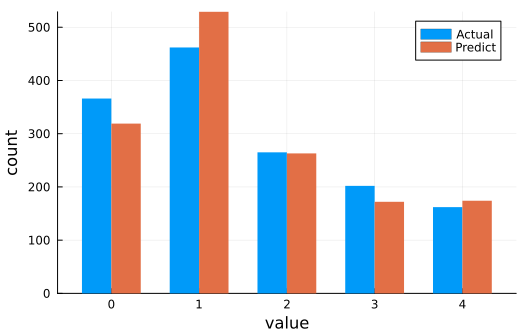
\includegraphics{./entry_exit_application_files/figure-pdf/cell-16-output-1.svg}

}

\end{figure}

\hypertarget{section-26}{%
\section{7}\label{section-26}}

\begin{Shaded}
\begin{Highlighting}[]
\NormalTok{data\_cf }\OperatorTok{=} \FunctionTok{copy}\NormalTok{(data\_processed);}
\FunctionTok{sort!}\NormalTok{(data\_cf, [}\OperatorTok{:}\NormalTok{CityCode, }\OperatorTok{:}\NormalTok{DepNeurology, }\OperatorTok{:}\NormalTok{DepNeurosurgery, }\OperatorTok{:}\NormalTok{LogNumBeds, }\OperatorTok{:}\NormalTok{TieEntryOrder], rev }\OperatorTok{=}\NormalTok{ [}\ConstantTok{false}\NormalTok{, }\ConstantTok{true}\NormalTok{, }\ConstantTok{true}\NormalTok{, }\ConstantTok{true}\NormalTok{, }\ConstantTok{true}\NormalTok{]);}
\FunctionTok{transform!}\NormalTok{(}\FunctionTok{groupby}\NormalTok{(data\_cf, }\OperatorTok{:}\NormalTok{CityCode), }\OperatorTok{:}\NormalTok{NumPotenHos }\OperatorTok{=\textgreater{}}\NormalTok{ (x }\OperatorTok{{-}\textgreater{}} \FloatTok{1}\OperatorTok{:}\FunctionTok{length}\NormalTok{(x)) }\OperatorTok{=\textgreater{}} \OperatorTok{:}\NormalTok{EntryOrderId);}
\NormalTok{var\_profit\_cf }\OperatorTok{=} \FunctionTok{Matrix}\NormalTok{(data\_cf[}\OperatorTok{:}\NormalTok{, [}\OperatorTok{:}\NormalTok{Const, }\OperatorTok{:}\NormalTok{Menseki, }\OperatorTok{:}\NormalTok{LogPop, }\OperatorTok{:}\NormalTok{LogIncome]]) }\OperatorTok{*}\NormalTok{ beta\_est }\OperatorTok{.+} 
\NormalTok{    rho\_est }\OperatorTok{.*}\NormalTok{ u\_m0;}
\NormalTok{fixed\_cost\_cf }\OperatorTok{=} \FunctionTok{Matrix}\NormalTok{(data\_cf[}\OperatorTok{:}\NormalTok{, [}\OperatorTok{:}\NormalTok{Kyukyu, }\OperatorTok{:}\NormalTok{Sien, }\OperatorTok{:}\NormalTok{Hyoka, }\OperatorTok{:}\NormalTok{DepNeurology, }\OperatorTok{:}\NormalTok{DepNeurosurgery, }\OperatorTok{:}\NormalTok{LogNumBeds, }\OperatorTok{:}\NormalTok{ZeroBedDum, }\OperatorTok{:}\NormalTok{DaigakuDum]]) }\OperatorTok{*}\NormalTok{ alpha\_est }\OperatorTok{.{-}}
\NormalTok{    (}\FunctionTok{sqrt}\NormalTok{.(}\FloatTok{1.0} \OperatorTok{{-}}\NormalTok{ rho\_est}\OperatorTok{\^{}}\FloatTok{2}\NormalTok{) }\OperatorTok{.*}\NormalTok{ u\_mIm);}

\NormalTok{prof\_excl\_comp\_cf }\OperatorTok{=}\NormalTok{ var\_profit\_cf }\OperatorTok{{-}}\NormalTok{ fixed\_cost\_cf;}
\NormalTok{prof\_excl\_comp\_cf[(data\_cf.DepNeurology }\OperatorTok{.==} \FloatTok{1}\NormalTok{) }\OperatorTok{.|}\NormalTok{ (data\_cf.DepNeurosurgery }\OperatorTok{.==} \FloatTok{1}\NormalTok{), }\OperatorTok{:}\NormalTok{] }\OperatorTok{.=} \FloatTok{1e+5}\NormalTok{;}
\end{Highlighting}
\end{Shaded}

\begin{Shaded}
\begin{Highlighting}[]
\NormalTok{EntryProb\_cf }\OperatorTok{=} \FunctionTok{map}\NormalTok{(}
\NormalTok{    i }\OperatorTok{{-}\textgreater{}} \FunctionTok{entry\_sim}\NormalTok{(data\_cf[data\_cf.CityCode }\OperatorTok{.==}\NormalTok{ i, }\OperatorTok{:}\NormalTok{], delta\_est, prof\_excl\_comp\_cf[data\_cf.CityCode }\OperatorTok{.==}\NormalTok{ i, }\OperatorTok{:}\NormalTok{]), }
\NormalTok{    uniqueCityCode}
\NormalTok{);}
\end{Highlighting}
\end{Shaded}

\begin{Shaded}
\begin{Highlighting}[]
\NormalTok{EntryPred\_cf }\OperatorTok{=} \FunctionTok{reduce}\NormalTok{(vcat, EntryProb\_cf) }\OperatorTok{.\textgreater{}} \FloatTok{0.5}\NormalTok{;}
\NormalTok{data\_predicted\_cf }\OperatorTok{=} \FunctionTok{copy}\NormalTok{(data\_processed);}
\NormalTok{data\_predicted\_cf[!, }\OperatorTok{:}\NormalTok{EntryProb] }\OperatorTok{=} \FunctionTok{reduce}\NormalTok{(vcat, EntryProb\_cf);}
\NormalTok{data\_predicted\_cf[!, }\OperatorTok{:}\NormalTok{EntryPred] }\OperatorTok{=}\NormalTok{ EntryPred\_cf;}
\NormalTok{data\_predicted\_cf\_agg }\OperatorTok{=} \FunctionTok{combine}\NormalTok{(}
    \FunctionTok{groupby}\NormalTok{(data\_predicted\_cf, }\OperatorTok{:}\NormalTok{CityCode),}
    \OperatorTok{:}\NormalTok{MRIOwnDum }\OperatorTok{=\textgreater{}}\NormalTok{ sum }\OperatorTok{=\textgreater{}} \OperatorTok{:}\NormalTok{Actual,}
    \OperatorTok{:}\NormalTok{EntryPred }\OperatorTok{=\textgreater{}}\NormalTok{ sum }\OperatorTok{=\textgreater{}} \OperatorTok{:}\NormalTok{CounterFactual}
\NormalTok{);}

\NormalTok{data\_predicted\_cf\_agg }\OperatorTok{=} \FunctionTok{stack}\NormalTok{(data\_predicted\_cf\_agg, [}\OperatorTok{:}\NormalTok{Actual, }\OperatorTok{:}\NormalTok{CounterFactual]);}
\NormalTok{data\_predicted\_cf\_sum }\OperatorTok{=} \FunctionTok{combine}\NormalTok{(}\FunctionTok{groupby}\NormalTok{(}
    \FunctionTok{vcat}\NormalTok{(data\_predicted\_agg, data\_predicted\_cf\_agg[data\_predicted\_cf\_agg.variable }\OperatorTok{.==} \StringTok{"CounterFactual"}\NormalTok{, }\OperatorTok{:}\NormalTok{]),}
\NormalTok{    [}\OperatorTok{:}\NormalTok{variable, }\OperatorTok{:}\NormalTok{value]}
\NormalTok{    ), nrow);}

\FunctionTok{transform!}\NormalTok{(}
\NormalTok{    data\_predicted\_cf\_sum, }
    \OperatorTok{:}\NormalTok{variable }\OperatorTok{=\textgreater{}} 
\NormalTok{    (x }\OperatorTok{{-}\textgreater{}} \FunctionTok{categorical}\NormalTok{(x; ordered }\OperatorTok{=} \ConstantTok{true}\NormalTok{, levels }\OperatorTok{=}\NormalTok{ [}\StringTok{"Actual"}\NormalTok{, }\StringTok{"Predict"}\NormalTok{, }\StringTok{"CounterFactual"}\NormalTok{])) }\OperatorTok{=\textgreater{}} 
    \OperatorTok{:}\NormalTok{variable}
\NormalTok{    )}
\FunctionTok{sort!}\NormalTok{(data\_predicted\_cf\_sum, [}\OperatorTok{:}\NormalTok{variable, }\OperatorTok{:}\NormalTok{value]);}
\FunctionTok{groupedbar}\NormalTok{(}
\NormalTok{    data\_predicted\_cf\_sum.nrow, }
\NormalTok{    group }\OperatorTok{=}\NormalTok{ data\_predicted\_cf\_sum.variable,}
\NormalTok{    xlabel }\OperatorTok{=} \StringTok{"value"}\NormalTok{, }
\NormalTok{    ylabel }\OperatorTok{=} \StringTok{"count"}\NormalTok{,}
\NormalTok{    bar\_width }\OperatorTok{=} \FloatTok{0.67}\NormalTok{,}
\NormalTok{    xticks }\OperatorTok{=}\NormalTok{ (}\FloatTok{1}\OperatorTok{:}\FloatTok{5}\NormalTok{, }\FloatTok{0}\OperatorTok{:}\FloatTok{4}\NormalTok{),}
\NormalTok{    lw }\OperatorTok{=} \FloatTok{0}
\NormalTok{)}
\end{Highlighting}
\end{Shaded}

\begin{figure}[H]

{\centering 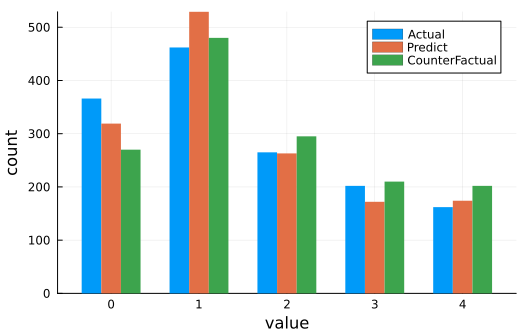
\includegraphics{./entry_exit_application_files/figure-pdf/cell-20-output-1.svg}

}

\end{figure}

\begin{Shaded}
\begin{Highlighting}[]
\FunctionTok{vcat}\NormalTok{(}
    \FunctionTok{combine}\NormalTok{(}\FunctionTok{groupby}\NormalTok{(}
\NormalTok{        data\_predicted\_agg, }\OperatorTok{:}\NormalTok{variable}
\NormalTok{        ), }\OperatorTok{:}\NormalTok{value }\OperatorTok{=\textgreater{}}\NormalTok{ sum),}
    \FunctionTok{combine}\NormalTok{(}\FunctionTok{groupby}\NormalTok{(}
\NormalTok{        data\_predicted\_cf\_agg, }\OperatorTok{:}\NormalTok{variable}
\NormalTok{        ), }\OperatorTok{:}\NormalTok{value }\OperatorTok{=\textgreater{}}\NormalTok{ sum) }\OperatorTok{|\textgreater{}} 
        \FunctionTok{filter}\NormalTok{(}\OperatorTok{:}\NormalTok{variable }\OperatorTok{=\textgreater{}}\NormalTok{ (x }\OperatorTok{{-}\textgreater{}}\NormalTok{ x }\OperatorTok{.==} \StringTok{"CounterFactual"}\NormalTok{))}
\NormalTok{)}
\end{Highlighting}
\end{Shaded}

\begin{tabular}{r|cc}
    & variable & value\_sum\\
    \hline
    & String & Int64\\
    \hline
    1 & Actual & 2246 \\
    2 & Predict & 2267 \\
    3 & CounterFactual & 2508 \\
\end{tabular}

\begin{Shaded}
\begin{Highlighting}[]
\NormalTok{data\_predicted\_agg\_wo\_neuro }\OperatorTok{=} \FunctionTok{combine}\NormalTok{(}
    \FunctionTok{groupby}\NormalTok{(}
        \FunctionTok{filter}\NormalTok{([}\OperatorTok{:}\NormalTok{DepNeurology, }\OperatorTok{:}\NormalTok{DepNeurosurgery] }\OperatorTok{=\textgreater{}}\NormalTok{ ((d1, d2) }\OperatorTok{{-}\textgreater{}}\NormalTok{ (d1 }\OperatorTok{.==} \FloatTok{1}\NormalTok{) }\OperatorTok{.\&}\NormalTok{ (d2 }\OperatorTok{.==} \FloatTok{1}\NormalTok{)), data\_predicted),}
        \OperatorTok{:}\NormalTok{CityCode}
\NormalTok{        ),}
    \OperatorTok{:}\NormalTok{MRIOwnDum }\OperatorTok{=\textgreater{}}\NormalTok{ sum }\OperatorTok{=\textgreater{}} \OperatorTok{:}\NormalTok{Actual,}
    \OperatorTok{:}\NormalTok{EntryPred }\OperatorTok{=\textgreater{}}\NormalTok{ sum }\OperatorTok{=\textgreater{}} \OperatorTok{:}\NormalTok{Predict}
\NormalTok{);}

\NormalTok{data\_predicted\_agg\_wo\_neuro }\OperatorTok{=} \FunctionTok{stack}\NormalTok{(data\_predicted\_agg\_wo\_neuro, [}\OperatorTok{:}\NormalTok{Actual, }\OperatorTok{:}\NormalTok{Predict]);}
\NormalTok{data\_predicted\_sum\_wo\_neuro }\OperatorTok{=} \FunctionTok{combine}\NormalTok{(}\FunctionTok{groupby}\NormalTok{(data\_predicted\_agg\_wo\_neuro, [}\OperatorTok{:}\NormalTok{variable, }\OperatorTok{:}\NormalTok{value]), nrow);}

\NormalTok{data\_predicted\_cf\_agg\_wo\_neuro }\OperatorTok{=} \FunctionTok{combine}\NormalTok{(}
    \FunctionTok{groupby}\NormalTok{(}
        \CommentTok{\# data\_predicted\_cf, }
        \FunctionTok{filter}\NormalTok{([}\OperatorTok{:}\NormalTok{DepNeurology, }\OperatorTok{:}\NormalTok{DepNeurosurgery] }\OperatorTok{=\textgreater{}}\NormalTok{ ((d1, d2) }\OperatorTok{{-}\textgreater{}}\NormalTok{ (d1 }\OperatorTok{.==} \FloatTok{1}\NormalTok{) }\OperatorTok{.\&}\NormalTok{ (d2 }\OperatorTok{.==} \FloatTok{1}\NormalTok{)), data\_predicted\_cf),}
        \OperatorTok{:}\NormalTok{CityCode}
\NormalTok{        ),}
    \OperatorTok{:}\NormalTok{MRIOwnDum }\OperatorTok{=\textgreater{}}\NormalTok{ sum }\OperatorTok{=\textgreater{}} \OperatorTok{:}\NormalTok{Actual,}
    \OperatorTok{:}\NormalTok{EntryPred }\OperatorTok{=\textgreater{}}\NormalTok{ sum }\OperatorTok{=\textgreater{}} \OperatorTok{:}\NormalTok{CounterFactual}
\NormalTok{);}

\NormalTok{data\_predicted\_cf\_agg\_wo\_neuro }\OperatorTok{=} \FunctionTok{stack}\NormalTok{(data\_predicted\_cf\_agg\_wo\_neuro, [}\OperatorTok{:}\NormalTok{Actual, }\OperatorTok{:}\NormalTok{CounterFactual]);}

\NormalTok{data\_predicted\_cf\_sum\_wo\_neuro }\OperatorTok{=} \FunctionTok{combine}\NormalTok{(}\FunctionTok{groupby}\NormalTok{(}
    \FunctionTok{vcat}\NormalTok{(}
\NormalTok{        data\_predicted\_agg\_wo\_neuro, }
\NormalTok{        data\_predicted\_cf\_agg\_wo\_neuro[data\_predicted\_cf\_agg\_wo\_neuro.variable }\OperatorTok{.==} \StringTok{"CounterFactual"}\NormalTok{, }\OperatorTok{:}\NormalTok{]}
\NormalTok{        ),}
\NormalTok{    [}\OperatorTok{:}\NormalTok{variable, }\OperatorTok{:}\NormalTok{value]}
\NormalTok{    ), nrow)}

\FunctionTok{transform!}\NormalTok{(}
\NormalTok{    data\_predicted\_cf\_sum\_wo\_neuro, }
    \OperatorTok{:}\NormalTok{variable }\OperatorTok{=\textgreater{}} 
\NormalTok{    (x }\OperatorTok{{-}\textgreater{}} \FunctionTok{categorical}\NormalTok{(x; ordered }\OperatorTok{=} \ConstantTok{true}\NormalTok{, levels }\OperatorTok{=}\NormalTok{ [}\StringTok{"Actual"}\NormalTok{, }\StringTok{"Predict"}\NormalTok{, }\StringTok{"CounterFactual"}\NormalTok{])) }\OperatorTok{=\textgreater{}} 
    \OperatorTok{:}\NormalTok{variable}
\NormalTok{    )}
\FunctionTok{sort!}\NormalTok{(data\_predicted\_cf\_sum\_wo\_neuro, [}\OperatorTok{:}\NormalTok{variable, }\OperatorTok{:}\NormalTok{value]);}
\FunctionTok{groupedbar}\NormalTok{(}
\NormalTok{    data\_predicted\_cf\_sum\_wo\_neuro.nrow, }
\NormalTok{    group }\OperatorTok{=}\NormalTok{ data\_predicted\_cf\_sum\_wo\_neuro.variable,}
\NormalTok{    xlabel }\OperatorTok{=} \StringTok{"value"}\NormalTok{, }
\NormalTok{    ylabel }\OperatorTok{=} \StringTok{"count"}\NormalTok{,}
\NormalTok{    bar\_width }\OperatorTok{=} \FloatTok{0.67}\NormalTok{,}
\NormalTok{    xticks }\OperatorTok{=}\NormalTok{ (}\FloatTok{1}\OperatorTok{:}\FloatTok{5}\NormalTok{, }\FloatTok{0}\OperatorTok{:}\FloatTok{4}\NormalTok{),}
\NormalTok{    lw }\OperatorTok{=} \FloatTok{0}
\NormalTok{)}
\end{Highlighting}
\end{Shaded}

\begin{figure}[H]

{\centering 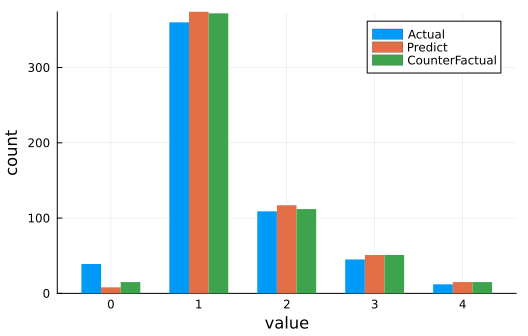
\includegraphics{./entry_exit_application_files/figure-pdf/cell-22-output-1.svg}

}

\end{figure}

\begin{Shaded}
\begin{Highlighting}[]
\FunctionTok{vcat}\NormalTok{(}
    \FunctionTok{combine}\NormalTok{(}\FunctionTok{groupby}\NormalTok{(}
\NormalTok{        data\_predicted\_agg\_wo\_neuro, }\OperatorTok{:}\NormalTok{variable}
\NormalTok{        ), }\OperatorTok{:}\NormalTok{value }\OperatorTok{=\textgreater{}}\NormalTok{ sum),}
    \FunctionTok{combine}\NormalTok{(}\FunctionTok{groupby}\NormalTok{(}
\NormalTok{        data\_predicted\_cf\_agg\_wo\_neuro, }\OperatorTok{:}\NormalTok{variable}
\NormalTok{        ), }\OperatorTok{:}\NormalTok{value }\OperatorTok{=\textgreater{}}\NormalTok{ sum) }\OperatorTok{|\textgreater{}} 
        \FunctionTok{filter}\NormalTok{(}\OperatorTok{:}\NormalTok{variable }\OperatorTok{=\textgreater{}}\NormalTok{ (x }\OperatorTok{{-}\textgreater{}}\NormalTok{ x }\OperatorTok{.==} \StringTok{"CounterFactual"}\NormalTok{))}
\NormalTok{)}
\end{Highlighting}
\end{Shaded}

\begin{tabular}{r|cc}
    & variable & value\_sum\\
    \hline
    & String & Int64\\
    \hline
    1 & Actual & 761 \\
    2 & Predict & 821 \\
    3 & CounterFactual & 809 \\
\end{tabular}

\bookmarksetup{startatroot}

\hypertarget{ux30b7ux30f3ux30b0ux30ebux30a8ux30fcux30b8ux30a7ux30f3ux30c8ux52d5ux5b66ux30e2ux30c7ux30ebux306eux63a8ux5b9aux57faux790eux7de8}{%
\chapter{シングルエージェント動学モデルの推定(基礎編)}\label{ux30b7ux30f3ux30b0ux30ebux30a8ux30fcux30b8ux30a7ux30f3ux30c8ux52d5ux5b66ux30e2ux30c7ux30ebux306eux63a8ux5b9aux57faux790eux7de8}}

\begin{Shaded}
\begin{Highlighting}[]
\ImportTok{using} \BuiltInTok{LinearAlgebra}
\ImportTok{using} \BuiltInTok{Random}
\ImportTok{using} \BuiltInTok{StatsBase}
\ImportTok{using} \BuiltInTok{Distributions}
\ImportTok{using} \BuiltInTok{DataFrames}
\ImportTok{using} \BuiltInTok{Plots}
\ImportTok{using} \BuiltInTok{ShiftedArrays}
\ImportTok{using} \BuiltInTok{ForwardDiff}
\ImportTok{using} \BuiltInTok{Optim}
\end{Highlighting}
\end{Shaded}

\begin{Shaded}
\begin{Highlighting}[]
\NormalTok{theta\_true }\OperatorTok{=}\NormalTok{ [}\FloatTok{0.004}\NormalTok{, }\FloatTok{0.003}\NormalTok{]}

\NormalTok{beta }\OperatorTok{=} \FloatTok{0.99}\NormalTok{;}
\NormalTok{Euler\_const }\OperatorTok{=} \FunctionTok{Float64}\NormalTok{(}\BuiltInTok{MathConstants}\NormalTok{.}\ConstantTok{eulergamma}\NormalTok{);}

\NormalTok{num\_choice }\OperatorTok{=} \FloatTok{2}\NormalTok{;}
\end{Highlighting}
\end{Shaded}

\begin{Shaded}
\begin{Highlighting}[]
\NormalTok{price\_states }\OperatorTok{=} \FloatTok{2000}\OperatorTok{:}\FloatTok{100}\OperatorTok{:}\FloatTok{2500}\NormalTok{;}
\NormalTok{mileage\_states }\OperatorTok{=} \FloatTok{0}\OperatorTok{:}\FloatTok{5}\OperatorTok{:}\FloatTok{100}\NormalTok{;}
\NormalTok{num\_price\_states }\OperatorTok{=} \FunctionTok{length}\NormalTok{(price\_states);}
\NormalTok{num\_mileage\_states }\OperatorTok{=} \FunctionTok{length}\NormalTok{(mileage\_states);}
\NormalTok{num\_states }\OperatorTok{=}\NormalTok{ num\_price\_states }\OperatorTok{*}\NormalTok{ num\_mileage\_states;}

\NormalTok{states\_matrix }\OperatorTok{=} \FunctionTok{Matrix}\NormalTok{(}\FunctionTok{reshape}\NormalTok{(}\FunctionTok{reinterpret}\NormalTok{(}\DataTypeTok{Int}\NormalTok{, }\FunctionTok{collect}\NormalTok{(}\BuiltInTok{Iterators}\NormalTok{.}\FunctionTok{product}\NormalTok{(price\_states, mileage\_states))), (}\FloatTok{2}\NormalTok{, }\OperatorTok{:}\NormalTok{))}\CharTok{\textquotesingle{});}
\end{Highlighting}
\end{Shaded}

\begin{Shaded}
\begin{Highlighting}[]
\KeywordTok{function} \FunctionTok{gen\_mileage\_trans!}\NormalTok{(}
\NormalTok{    kappa}\OperatorTok{::}\DataTypeTok{Vector\{Float64\}}\NormalTok{,}
\NormalTok{    num\_mileage\_states}\OperatorTok{::}\DataTypeTok{Int}\NormalTok{,}
\NormalTok{    mileage\_trans\_mat}\OperatorTok{::}\DataTypeTok{Array\{Float64, 3\}}
\NormalTok{    )}
\NormalTok{    kappa\_1 }\OperatorTok{=}\NormalTok{ kappa[}\FloatTok{1}\NormalTok{];}
\NormalTok{    kappa\_2 }\OperatorTok{=}\NormalTok{ kappa[}\FloatTok{2}\NormalTok{];}

\NormalTok{    mileage\_trans\_mat[}\OperatorTok{:}\NormalTok{, }\OperatorTok{:}\NormalTok{, }\OperatorTok{:}\NormalTok{] }\OperatorTok{.=} \FloatTok{0}\NormalTok{;}
    \ControlFlowTok{for}\NormalTok{ i }\KeywordTok{in} \FloatTok{1}\OperatorTok{:}\NormalTok{num\_mileage\_states, j }\KeywordTok{in} \FloatTok{1}\OperatorTok{:}\NormalTok{num\_mileage\_states}
        \ControlFlowTok{if}\NormalTok{ (i }\OperatorTok{==}\NormalTok{ j)}
\NormalTok{            mileage\_trans\_mat[i, j, }\FloatTok{1}\NormalTok{] }\OperatorTok{=} \FloatTok{1} \OperatorTok{{-}}\NormalTok{ kappa\_1 }\OperatorTok{{-}}\NormalTok{ kappa\_2;}
        \ControlFlowTok{elseif}\NormalTok{ (i }\OperatorTok{==}\NormalTok{ j }\OperatorTok{{-}} \FloatTok{1}\NormalTok{)}
\NormalTok{            mileage\_trans\_mat[i, j, }\FloatTok{1}\NormalTok{] }\OperatorTok{=}\NormalTok{ kappa\_1;}
        \ControlFlowTok{elseif}\NormalTok{ (i }\OperatorTok{==}\NormalTok{ j }\OperatorTok{{-}} \FloatTok{2}\NormalTok{)}
\NormalTok{            mileage\_trans\_mat[i, j, }\FloatTok{1}\NormalTok{] }\OperatorTok{=}\NormalTok{ kappa\_2;}
        \ControlFlowTok{end}
    \ControlFlowTok{end}
\NormalTok{    mileage\_trans\_mat[num\_mileage\_states }\OperatorTok{{-}} \FloatTok{1}\NormalTok{, num\_mileage\_states, }\FloatTok{1}\NormalTok{] }\OperatorTok{=}\NormalTok{ kappa\_1 }\OperatorTok{+}\NormalTok{ kappa\_2;}
\NormalTok{    mileage\_trans\_mat[num\_mileage\_states, num\_mileage\_states, }\FloatTok{1}\NormalTok{] }\OperatorTok{=} \FloatTok{1}\NormalTok{;}

\NormalTok{    mileage\_trans\_mat[}\OperatorTok{:}\NormalTok{, }\OperatorTok{:}\NormalTok{, }\FloatTok{2}\NormalTok{] }\OperatorTok{=} \FunctionTok{repeat}\NormalTok{(mileage\_trans\_mat[}\FloatTok{1}\NormalTok{, }\OperatorTok{:}\NormalTok{, }\FloatTok{1}\NormalTok{]}\CharTok{\textquotesingle{}, num\_mileage\_states);}
\KeywordTok{end}
\end{Highlighting}
\end{Shaded}

\begin{verbatim}
gen_mileage_trans! (generic function with 1 method)
\end{verbatim}

\begin{Shaded}
\begin{Highlighting}[]
\NormalTok{kappa\_true }\OperatorTok{=}\NormalTok{ [}\FloatTok{0.25}\NormalTok{, }\FloatTok{0.05}\NormalTok{];}

\NormalTok{mileage\_trans\_mat\_true }\OperatorTok{=} \FunctionTok{zeros}\NormalTok{((num\_mileage\_states, num\_mileage\_states, num\_choice));}
\FunctionTok{gen\_mileage\_trans!}\NormalTok{(kappa\_true, num\_mileage\_states, mileage\_trans\_mat\_true);}

\NormalTok{mileage\_trans\_mat\_true[}\FloatTok{1}\OperatorTok{:}\FloatTok{4}\NormalTok{, }\FloatTok{1}\OperatorTok{:}\FloatTok{4}\NormalTok{, }\FloatTok{1}\NormalTok{]}
\end{Highlighting}
\end{Shaded}

\begin{verbatim}
4×4 Matrix{Float64}:
 0.7  0.25  0.05  0.0
 0.0  0.7   0.25  0.05
 0.0  0.0   0.7   0.25
 0.0  0.0   0.0   0.7
\end{verbatim}

\begin{Shaded}
\begin{Highlighting}[]
\KeywordTok{function} \FunctionTok{gen\_price\_trans!}\NormalTok{(}
\NormalTok{    lambda}\OperatorTok{::}\DataTypeTok{Vector\{Float64\}}\NormalTok{,}
\NormalTok{    num\_price\_states}\OperatorTok{::}\DataTypeTok{Int}\NormalTok{,}
\NormalTok{    price\_trans\_mat}\OperatorTok{::}\DataTypeTok{Array\{Float64, 2\}}
\NormalTok{    )}

\NormalTok{    price\_trans\_mat[}\OperatorTok{:}\NormalTok{, }\OperatorTok{:}\NormalTok{] }\OperatorTok{.=} \FloatTok{0}\NormalTok{;}

\NormalTok{    price\_trans\_mat[}\FloatTok{1}\NormalTok{, }\FloatTok{2}\OperatorTok{:}\KeywordTok{end}\NormalTok{] }\OperatorTok{=}\NormalTok{ lambda[}\FloatTok{1}\OperatorTok{:}\NormalTok{(num\_price\_states }\OperatorTok{{-}} \FloatTok{1}\NormalTok{)];}
\NormalTok{    price\_trans\_mat[}\FloatTok{1}\NormalTok{, }\FloatTok{1}\NormalTok{] }\OperatorTok{=} \FloatTok{1} \OperatorTok{{-}} \FunctionTok{sum}\NormalTok{(price\_trans\_mat[}\FloatTok{1}\NormalTok{, }\OperatorTok{:}\NormalTok{]);}

    \ControlFlowTok{for}\NormalTok{ i }\KeywordTok{in} \FloatTok{2}\OperatorTok{:}\NormalTok{(num\_price\_states }\OperatorTok{{-}} \FloatTok{1}\NormalTok{)}
\NormalTok{        price\_trans\_mat[i, }\FloatTok{1}\OperatorTok{:}\NormalTok{(i }\OperatorTok{{-}} \FloatTok{1}\NormalTok{)] }\OperatorTok{=}\NormalTok{ lambda[}
\NormalTok{            ((i }\OperatorTok{{-}} \FloatTok{1}\NormalTok{) }\OperatorTok{*}\NormalTok{ (num\_price\_states }\OperatorTok{{-}} \FloatTok{1}\NormalTok{) }\OperatorTok{+} \FloatTok{1}\NormalTok{)}\OperatorTok{:}\NormalTok{((i }\OperatorTok{{-}} \FloatTok{1}\NormalTok{) }\OperatorTok{*}\NormalTok{ (num\_price\_states }\OperatorTok{{-}} \FloatTok{1}\NormalTok{) }\OperatorTok{+}\NormalTok{ (i }\OperatorTok{{-}} \FloatTok{1}\NormalTok{))}
\NormalTok{            ];}
\NormalTok{        price\_trans\_mat[i, (i }\OperatorTok{+} \FloatTok{1}\NormalTok{)}\OperatorTok{:}\KeywordTok{end}\NormalTok{] }\OperatorTok{=}\NormalTok{ lambda[}
\NormalTok{            ((i }\OperatorTok{{-}} \FloatTok{1}\NormalTok{) }\OperatorTok{*}\NormalTok{ (num\_price\_states }\OperatorTok{{-}} \FloatTok{1}\NormalTok{) }\OperatorTok{+}\NormalTok{ i)}\OperatorTok{:}\NormalTok{(i }\OperatorTok{*}\NormalTok{ (num\_price\_states }\OperatorTok{{-}} \FloatTok{1}\NormalTok{))}
\NormalTok{            ];}
\NormalTok{        price\_trans\_mat[i, i] }\OperatorTok{=} \FloatTok{1} \OperatorTok{{-}} \FunctionTok{sum}\NormalTok{(price\_trans\_mat[i, }\OperatorTok{:}\NormalTok{]);}
    \ControlFlowTok{end}

\NormalTok{    price\_trans\_mat[num\_price\_states, }\FloatTok{1}\OperatorTok{:}\NormalTok{(}\KeywordTok{end} \OperatorTok{{-}} \FloatTok{1}\NormalTok{)] }\OperatorTok{=}\NormalTok{ lambda[((num\_price\_states }\OperatorTok{{-}} \FloatTok{1}\NormalTok{) }\OperatorTok{*}\NormalTok{ (num\_price\_states }\OperatorTok{{-}} \FloatTok{1}\NormalTok{) }\OperatorTok{+} \FloatTok{1}\NormalTok{)}\OperatorTok{:}\KeywordTok{end}\NormalTok{];}
\NormalTok{    price\_trans\_mat[num\_price\_states, num\_price\_states] }\OperatorTok{=} \FloatTok{1} \OperatorTok{{-}} \FunctionTok{sum}\NormalTok{(price\_trans\_mat[num\_price\_states, }\OperatorTok{:}\NormalTok{]);}

\KeywordTok{end}
\end{Highlighting}
\end{Shaded}

\begin{verbatim}
gen_price_trans! (generic function with 1 method)
\end{verbatim}

\begin{Shaded}
\begin{Highlighting}[]
\NormalTok{lambda\_true }\OperatorTok{=}\NormalTok{ [}
    \FloatTok{0.1}\NormalTok{, }\FloatTok{0.2}\NormalTok{, }\FloatTok{0.2}\NormalTok{, }\FloatTok{0.2}\NormalTok{, }\FloatTok{0.2}\NormalTok{,}
    \FloatTok{0.1}\NormalTok{, }\FloatTok{0.2}\NormalTok{, }\FloatTok{0.2}\NormalTok{, }\FloatTok{0.2}\NormalTok{, }\FloatTok{0.2}\NormalTok{,}
    \FloatTok{0.1}\NormalTok{, }\FloatTok{0.1}\NormalTok{, }\FloatTok{0.2}\NormalTok{, }\FloatTok{0.2}\NormalTok{, }\FloatTok{0.1}\NormalTok{,}
    \FloatTok{0.1}\NormalTok{, }\FloatTok{0.1}\NormalTok{, }\FloatTok{0.2}\NormalTok{, }\FloatTok{0.2}\NormalTok{, }\FloatTok{0.1}\NormalTok{,}
    \FloatTok{0.05}\NormalTok{, }\FloatTok{0.05}\NormalTok{, }\FloatTok{0.1}\NormalTok{, }\FloatTok{0.1}\NormalTok{, }\FloatTok{0.2}\NormalTok{,}
    \FloatTok{0.05}\NormalTok{, }\FloatTok{0.05}\NormalTok{, }\FloatTok{0.1}\NormalTok{, }\FloatTok{0.1}\NormalTok{, }\FloatTok{0.2}
\NormalTok{];}

\NormalTok{price\_trans\_mat\_true }\OperatorTok{=} \FunctionTok{zeros}\NormalTok{(num\_price\_states, num\_price\_states);}
\FunctionTok{gen\_price\_trans!}\NormalTok{(lambda\_true, num\_price\_states, price\_trans\_mat\_true);}
\end{Highlighting}
\end{Shaded}

\begin{Shaded}
\begin{Highlighting}[]
\NormalTok{trans\_mat\_true }\OperatorTok{=} \FunctionTok{Array}\DataTypeTok{\{Float64\}}\NormalTok{(}\ConstantTok{undef}\NormalTok{, num\_states, num\_states, num\_choice);}
\ControlFlowTok{for}\NormalTok{ i }\KeywordTok{in} \FloatTok{1}\OperatorTok{:}\NormalTok{num\_choice}
\NormalTok{    trans\_mat\_true[}\OperatorTok{:}\NormalTok{, }\OperatorTok{:}\NormalTok{, i] }\OperatorTok{=} \FunctionTok{kron}\NormalTok{(mileage\_trans\_mat\_true[}\OperatorTok{:}\NormalTok{, }\OperatorTok{:}\NormalTok{, i], price\_trans\_mat\_true);}
\ControlFlowTok{end}
\end{Highlighting}
\end{Shaded}

\begin{Shaded}
\begin{Highlighting}[]
\NormalTok{price\_trans\_eigen }\OperatorTok{=} \FunctionTok{eigvecs}\NormalTok{(price\_trans\_mat\_true}\OperatorTok{\textquotesingle{}}\NormalTok{);}
\NormalTok{price\_dist\_steady }\OperatorTok{=}\NormalTok{ price\_trans\_eigen[}\OperatorTok{:}\NormalTok{, }\KeywordTok{end}\NormalTok{] }\OperatorTok{/} \FunctionTok{sum}\NormalTok{(price\_trans\_eigen[}\OperatorTok{:}\NormalTok{, }\KeywordTok{end}\NormalTok{])}
\end{Highlighting}
\end{Shaded}

\begin{verbatim}
6-element Vector{Float64}:
 0.07377049180327863
 0.07377049180327883
 0.1639344262295082
 0.16393442622950818
 0.28571428571428564
 0.23887587822014061
\end{verbatim}

\begin{Shaded}
\begin{Highlighting}[]
\KeywordTok{function} \FunctionTok{flow\_utility}\NormalTok{(}
\NormalTok{    theta,}
\NormalTok{    states\_matrix}\OperatorTok{::}\DataTypeTok{Matrix\{Int\}}
\NormalTok{    )}

\NormalTok{    theta\_c }\OperatorTok{=}\NormalTok{ theta[}\FloatTok{1}\NormalTok{];}
\NormalTok{    theta\_p }\OperatorTok{=}\NormalTok{ theta[}\FloatTok{2}\NormalTok{];}

    \ControlFlowTok{return} \FunctionTok{hcat}\NormalTok{(}
        \OperatorTok{{-}}\NormalTok{ theta\_c }\OperatorTok{.*}\NormalTok{ states\_matrix[}\OperatorTok{:}\NormalTok{, }\FloatTok{2}\NormalTok{],}
        \OperatorTok{{-}}\NormalTok{ theta\_p }\OperatorTok{.*}\NormalTok{ states\_matrix[}\OperatorTok{:}\NormalTok{, }\FloatTok{1}\NormalTok{]}
\NormalTok{    );}
\KeywordTok{end}
\end{Highlighting}
\end{Shaded}

\begin{verbatim}
flow_utility (generic function with 1 method)
\end{verbatim}

\begin{Shaded}
\begin{Highlighting}[]
\KeywordTok{function} \FunctionTok{contraction}\NormalTok{(}
\NormalTok{    theta,}
\NormalTok{    beta}\OperatorTok{::}\DataTypeTok{Float64}\NormalTok{,}
\NormalTok{    trans\_mat}\OperatorTok{::}\DataTypeTok{Array\{Float64, 3\}}\NormalTok{,}
\NormalTok{    states\_matrix}\OperatorTok{::}\DataTypeTok{Matrix\{Int\}}\NormalTok{;}
\NormalTok{    num\_states}\OperatorTok{::}\DataTypeTok{Int }\OperatorTok{=}\NormalTok{ num\_states,}
\NormalTok{    num\_choice}\OperatorTok{::}\DataTypeTok{Int }\OperatorTok{=}\NormalTok{ num\_choice,}
\NormalTok{    Euler\_const}\OperatorTok{::}\DataTypeTok{Float64 }\OperatorTok{=}\NormalTok{ Euler\_const}
\NormalTok{    )}

\NormalTok{    U }\OperatorTok{=} \FunctionTok{flow\_utility}\NormalTok{(theta, states\_matrix);}

\NormalTok{    EV\_old }\OperatorTok{=} \FunctionTok{zeros}\NormalTok{((num\_states, num\_choice));}

\NormalTok{    diff }\OperatorTok{=} \FloatTok{1000}\NormalTok{;}
\NormalTok{    tol\_level }\OperatorTok{=} \FloatTok{1e{-}10}\NormalTok{;}

    \ControlFlowTok{while}\NormalTok{ (diff }\OperatorTok{\textgreater{}}\NormalTok{ tol\_level)}
\NormalTok{        EV\_new }\OperatorTok{=} \FunctionTok{hcat}\NormalTok{(}
\NormalTok{            Euler\_const }\OperatorTok{.+}\NormalTok{ trans\_mat[}\OperatorTok{:}\NormalTok{, }\OperatorTok{:}\NormalTok{, }\FloatTok{1}\NormalTok{] }\OperatorTok{*} \FunctionTok{log}\NormalTok{.(}\FunctionTok{sum}\NormalTok{(}\FunctionTok{exp}\NormalTok{.(U }\OperatorTok{.+}\NormalTok{ beta }\OperatorTok{.*}\NormalTok{ EV\_old), dims }\OperatorTok{=} \FloatTok{2}\NormalTok{)),}
\NormalTok{            Euler\_const }\OperatorTok{.+}\NormalTok{ trans\_mat[}\OperatorTok{:}\NormalTok{, }\OperatorTok{:}\NormalTok{, }\FloatTok{2}\NormalTok{] }\OperatorTok{*} \FunctionTok{log}\NormalTok{.(}\FunctionTok{sum}\NormalTok{(}\FunctionTok{exp}\NormalTok{.(U }\OperatorTok{.+}\NormalTok{ beta }\OperatorTok{.*}\NormalTok{ EV\_old), dims }\OperatorTok{=} \FloatTok{2}\NormalTok{))}
\NormalTok{        );}

\NormalTok{        diff }\OperatorTok{=} \FunctionTok{sum}\NormalTok{(}\FunctionTok{abs}\NormalTok{.(EV\_new }\OperatorTok{{-}}\NormalTok{ EV\_old));}

\NormalTok{        EV\_old }\OperatorTok{=}\NormalTok{ EV\_new[}\OperatorTok{:}\NormalTok{, }\OperatorTok{:}\NormalTok{];}
    \ControlFlowTok{end}

    \ControlFlowTok{return}\NormalTok{ EV\_old}

\KeywordTok{end}
\end{Highlighting}
\end{Shaded}

\begin{verbatim}
contraction (generic function with 1 method)
\end{verbatim}

\begin{Shaded}
\begin{Highlighting}[]
\PreprocessorTok{@time}\NormalTok{ EV\_true }\OperatorTok{=} \FunctionTok{contraction}\NormalTok{(theta\_true, beta, trans\_mat\_true, states\_matrix);}
\end{Highlighting}
\end{Shaded}

\begin{verbatim}
  0.700188 seconds (1.93 M allocations: 845.940 MiB, 11.70% gc time, 74.94% compilation time)
\end{verbatim}

\begin{Shaded}
\begin{Highlighting}[]
\NormalTok{U\_true }\OperatorTok{=} \FunctionTok{flow\_utility}\NormalTok{(theta\_true, states\_matrix);}
\NormalTok{V\_CS\_true }\OperatorTok{=}\NormalTok{ U\_true }\OperatorTok{+}\NormalTok{ beta }\OperatorTok{.*}\NormalTok{ EV\_true;}
\end{Highlighting}
\end{Shaded}

\begin{Shaded}
\begin{Highlighting}[]
\NormalTok{prob\_buy\_true\_mat }\OperatorTok{=} \FunctionTok{reshape}\NormalTok{(}
    \FunctionTok{exp}\NormalTok{.(V\_CS\_true[}\OperatorTok{:}\NormalTok{, }\FloatTok{2}\NormalTok{]) }\OperatorTok{./} \FunctionTok{sum}\NormalTok{(}\FunctionTok{exp}\NormalTok{.(V\_CS\_true), dims }\OperatorTok{=} \FloatTok{2}\NormalTok{), }
\NormalTok{    (num\_price\_states, num\_mileage\_states)}
\NormalTok{    )}
\end{Highlighting}
\end{Shaded}

\begin{verbatim}
6×21 Matrix{Float64}:
 0.00247262   0.00426036   0.00704966  …  0.27228    0.287275   0.297312
 0.00183294   0.00315964   0.00523208     0.217025   0.229939   0.238643
 0.00135852   0.00234232   0.00387998     0.167951   0.17849    0.185652
 0.00100677   0.00173635   0.0028775      0.130637   0.139257   0.145141
 0.000746029  0.00128747   0.00213568     0.105262   0.112684   0.117736
 0.000552779  0.000954177  0.00158333  …  0.0810209  0.0869503  0.0909947
\end{verbatim}

\begin{Shaded}
\begin{Highlighting}[]
\NormalTok{num\_consumer }\OperatorTok{=} \FloatTok{1000}\NormalTok{;}

\NormalTok{num\_period }\OperatorTok{=} \FloatTok{12} \OperatorTok{*} \FloatTok{50}\NormalTok{;}
\NormalTok{num\_period\_obs }\OperatorTok{=} \FloatTok{12} \OperatorTok{*} \FloatTok{10}\NormalTok{;}

\NormalTok{num\_obs }\OperatorTok{=}\NormalTok{ num\_consumer }\OperatorTok{*}\NormalTok{ num\_period;}
\end{Highlighting}
\end{Shaded}

\begin{Shaded}
\begin{Highlighting}[]
\BuiltInTok{Random}\NormalTok{.}\FunctionTok{seed!}\NormalTok{(}\FloatTok{42}\NormalTok{);}

\KeywordTok{function} \FunctionTok{generate\_data}\NormalTok{(}
\NormalTok{    consumer\_id}\OperatorTok{::}\DataTypeTok{Int}\NormalTok{,}
\NormalTok{    V\_CS}\OperatorTok{::}\DataTypeTok{Matrix\{Float64\}}\NormalTok{,}
\NormalTok{    trans\_mat}\OperatorTok{::}\DataTypeTok{Array\{Float64, 3\}}\NormalTok{,}
\NormalTok{    price\_dist\_steady}\OperatorTok{::}\DataTypeTok{Vector\{Float64\}}\NormalTok{;}
\NormalTok{    num\_period}\OperatorTok{::}\DataTypeTok{Int }\OperatorTok{=}\NormalTok{ num\_period,}
\NormalTok{)}

\NormalTok{    state\_vec }\OperatorTok{=} \FunctionTok{zeros}\NormalTok{(}\DataTypeTok{Int}\NormalTok{, num\_period);}
\NormalTok{    action\_vec }\OperatorTok{=} \FunctionTok{zeros}\NormalTok{(}\DataTypeTok{Int}\NormalTok{, num\_period);}
\NormalTok{    period\_vec }\OperatorTok{=} \FloatTok{1}\OperatorTok{:}\NormalTok{num\_period;}

\NormalTok{    eps\_type1 }\OperatorTok{=} \FunctionTok{reshape}\NormalTok{(}
        \FunctionTok{rand}\NormalTok{(}\FunctionTok{GeneralizedExtremeValue}\NormalTok{(}\FloatTok{0}\NormalTok{, }\FloatTok{1}\NormalTok{, }\FloatTok{0}\NormalTok{), num\_period }\OperatorTok{*} \FloatTok{2}\NormalTok{),}
\NormalTok{        (num\_period, }\FloatTok{2}\NormalTok{)}
\NormalTok{    );}

\NormalTok{    state\_vec[}\FloatTok{1}\NormalTok{] }\OperatorTok{=} \FunctionTok{sample}\NormalTok{(}\FunctionTok{ProbabilityWeights}\NormalTok{(price\_dist\_steady));}

    \ControlFlowTok{for}\NormalTok{ t }\KeywordTok{in} \FloatTok{1}\OperatorTok{:}\NormalTok{(num\_period }\OperatorTok{{-}} \FloatTok{1}\NormalTok{)}

\NormalTok{        state\_id\_today }\OperatorTok{=}\NormalTok{ state\_vec[t];}

        \ControlFlowTok{if}\NormalTok{ (}
\NormalTok{            V\_CS[}\OperatorTok{:}\NormalTok{, }\FloatTok{1}\NormalTok{][state\_id\_today] }\OperatorTok{+}\NormalTok{ eps\_type1[t, }\FloatTok{1}\NormalTok{] }\OperatorTok{\textgreater{}} 
\NormalTok{            V\_CS[}\OperatorTok{:}\NormalTok{, }\FloatTok{2}\NormalTok{][state\_id\_today] }\OperatorTok{+}\NormalTok{ eps\_type1[t, }\FloatTok{2}\NormalTok{]}
\NormalTok{            )}
\NormalTok{            action\_vec[t] }\OperatorTok{=} \FloatTok{0}\NormalTok{;}
\NormalTok{            state\_vec[t }\OperatorTok{+} \FloatTok{1}\NormalTok{] }\OperatorTok{=} \FunctionTok{sample}\NormalTok{(}
                \FunctionTok{ProbabilityWeights}\NormalTok{(trans\_mat[state\_id\_today, }\OperatorTok{:}\NormalTok{, }\FloatTok{1}\NormalTok{])}
\NormalTok{                );}
        \ControlFlowTok{else}
\NormalTok{            action\_vec[t] }\OperatorTok{=} \FloatTok{1}\NormalTok{;}
\NormalTok{            state\_vec[t }\OperatorTok{+} \FloatTok{1}\NormalTok{] }\OperatorTok{=} \FunctionTok{sample}\NormalTok{(}
                \FunctionTok{ProbabilityWeights}\NormalTok{(trans\_mat[state\_id\_today, }\OperatorTok{:}\NormalTok{, }\FloatTok{2}\NormalTok{])}
\NormalTok{                );}
        \ControlFlowTok{end}

    \ControlFlowTok{end}

    \ControlFlowTok{return} \FunctionTok{DataFrame}\NormalTok{(}
\NormalTok{        state }\OperatorTok{=}\NormalTok{ state\_vec, }
\NormalTok{        action }\OperatorTok{=}\NormalTok{ action\_vec, }
\NormalTok{        period }\OperatorTok{=}\NormalTok{ period\_vec,}
\NormalTok{        consumer\_id }\OperatorTok{=}\NormalTok{ consumer\_id}
\NormalTok{        )}
\KeywordTok{end}
\end{Highlighting}
\end{Shaded}

\begin{verbatim}
generate_data (generic function with 1 method)
\end{verbatim}

\begin{Shaded}
\begin{Highlighting}[]
\NormalTok{data\_gen }\OperatorTok{=} \FunctionTok{reduce}\NormalTok{(vcat, [}\FunctionTok{generate\_data}\NormalTok{(}
\NormalTok{    consumer\_id,}
\NormalTok{    V\_CS\_true,}
\NormalTok{    trans\_mat\_true,}
\NormalTok{    price\_dist\_steady}
\NormalTok{    ) for consumer\_id }\KeywordTok{in} \FloatTok{1}\OperatorTok{:}\NormalTok{num\_consumer]) }\OperatorTok{|\textgreater{}}
    \FunctionTok{filter}\NormalTok{(}\OperatorTok{:}\NormalTok{period }\OperatorTok{=\textgreater{}}\NormalTok{ (x }\OperatorTok{{-}\textgreater{}}\NormalTok{ x }\OperatorTok{\textgreater{}}\NormalTok{ num\_period }\OperatorTok{{-}}\NormalTok{ num\_period\_obs))}

\NormalTok{data\_gen[!, }\OperatorTok{:}\NormalTok{price] }\OperatorTok{=}\NormalTok{ states\_matrix[data\_gen.state, }\FloatTok{1}\NormalTok{];}
\NormalTok{data\_gen[!, }\OperatorTok{:}\NormalTok{mileage] }\OperatorTok{=}\NormalTok{ states\_matrix[data\_gen.state, }\FloatTok{2}\NormalTok{];}
\end{Highlighting}
\end{Shaded}

\begin{Shaded}
\begin{Highlighting}[]
\FunctionTok{describe}\NormalTok{(data\_gen[}\OperatorTok{:}\NormalTok{, [}\OperatorTok{:}\NormalTok{price, }\OperatorTok{:}\NormalTok{mileage, }\OperatorTok{:}\NormalTok{action]], }\OperatorTok{:}\NormalTok{all)[}\OperatorTok{:}\NormalTok{, [}\OperatorTok{:}\NormalTok{variable, }\OperatorTok{:}\NormalTok{mean, }\OperatorTok{:}\NormalTok{std, }\OperatorTok{:}\NormalTok{min, }\OperatorTok{:}\NormalTok{max]]}
\end{Highlighting}
\end{Shaded}

\begin{tabular}{r|ccccc}
    & variable & mean & std & min & max\\
    \hline
    & Symbol & Float64 & Float64 & Int64 & Int64\\
    \hline
    1 & price & 2322.63 & 151.826 & 2000 & 2500 \\
    2 & mileage & 33.0198 & 23.6924 & 0 & 100 \\
    3 & action & 0.02915 & 0.168228 & 0 & 1 \\
\end{tabular}

\begin{Shaded}
\begin{Highlighting}[]
\FunctionTok{histogram}\NormalTok{(data\_gen.price, bar\_width }\OperatorTok{=} \FloatTok{50}\NormalTok{, legend}\OperatorTok{=}\ConstantTok{false}\NormalTok{)}
\end{Highlighting}
\end{Shaded}

\begin{figure}[H]

{\centering 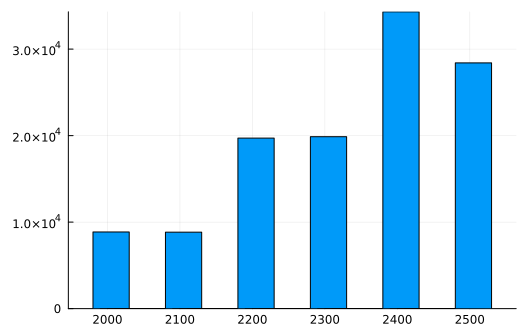
\includegraphics{./single_agent_dynamic_basic_files/figure-pdf/cell-20-output-1.svg}

}

\end{figure}

\begin{Shaded}
\begin{Highlighting}[]
\FunctionTok{histogram}\NormalTok{(data\_gen.mileage, bar\_width }\OperatorTok{=} \FloatTok{3}\NormalTok{, legend}\OperatorTok{=}\ConstantTok{false}\NormalTok{, bins }\OperatorTok{=}\NormalTok{ [}\FunctionTok{collect}\NormalTok{(mileage\_states); [}\FloatTok{105}\NormalTok{]] }\OperatorTok{.{-}} \FloatTok{2.5}\NormalTok{)}
\end{Highlighting}
\end{Shaded}

\begin{figure}[H]

{\centering 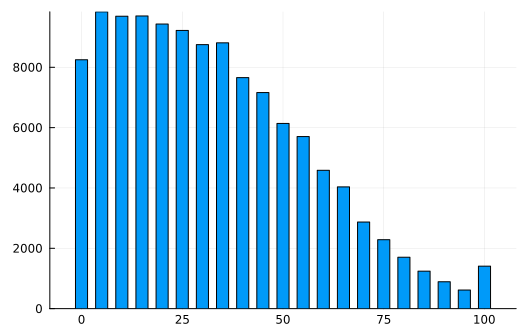
\includegraphics{./single_agent_dynamic_basic_files/figure-pdf/cell-21-output-1.svg}

}

\end{figure}

\begin{Shaded}
\begin{Highlighting}[]
\FunctionTok{bar}\NormalTok{(}
\NormalTok{    mileage\_states,}
    \FunctionTok{combine}\NormalTok{(}\FunctionTok{groupby}\NormalTok{(data\_gen, }\OperatorTok{:}\NormalTok{mileage), }\OperatorTok{:}\NormalTok{action }\OperatorTok{=\textgreater{}}\NormalTok{ mean).action\_mean,}
\NormalTok{    bar\_width }\OperatorTok{=} \FloatTok{3}\NormalTok{, legend}\OperatorTok{=}\ConstantTok{false}
\NormalTok{)}
\end{Highlighting}
\end{Shaded}

\begin{figure}[H]

{\centering 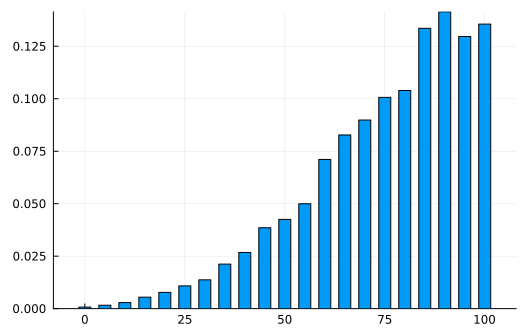
\includegraphics{./single_agent_dynamic_basic_files/figure-pdf/cell-22-output-1.svg}

}

\end{figure}

\begin{Shaded}
\begin{Highlighting}[]
\FunctionTok{bar}\NormalTok{(}
\NormalTok{    price\_states,}
    \FunctionTok{combine}\NormalTok{(}\FunctionTok{groupby}\NormalTok{(data\_gen, }\OperatorTok{:}\NormalTok{price), }\OperatorTok{:}\NormalTok{action }\OperatorTok{=\textgreater{}}\NormalTok{ mean).action\_mean,}
\NormalTok{    bar\_width }\OperatorTok{=} \FloatTok{50}\NormalTok{, legend}\OperatorTok{=}\ConstantTok{false}
\NormalTok{)}
\end{Highlighting}
\end{Shaded}

\begin{figure}[H]

{\centering 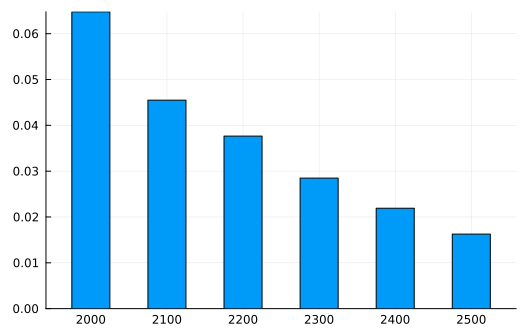
\includegraphics{./single_agent_dynamic_basic_files/figure-pdf/cell-23-output-1.svg}

}

\end{figure}

\begin{Shaded}
\begin{Highlighting}[]
\FunctionTok{surface}\NormalTok{(}
\NormalTok{    mileage\_states,}
\NormalTok{    price\_states,}
    \FunctionTok{reshape}\NormalTok{(}
        \FunctionTok{combine}\NormalTok{(}\FunctionTok{groupby}\NormalTok{(data\_gen, [}\OperatorTok{:}\NormalTok{mileage, }\OperatorTok{:}\NormalTok{price]), }\OperatorTok{:}\NormalTok{action }\OperatorTok{=\textgreater{}}\NormalTok{ mean).action\_mean, }
\NormalTok{        (num\_price\_states, num\_mileage\_states)}
\NormalTok{    ),}
\NormalTok{    xlabel }\OperatorTok{=} \StringTok{"Mileage"}\NormalTok{,}
\NormalTok{    ylabel }\OperatorTok{=} \StringTok{"Price"}\NormalTok{,}
\NormalTok{    zlabel }\OperatorTok{=} \StringTok{"Purchase prob."}\NormalTok{,}
\NormalTok{)}
\end{Highlighting}
\end{Shaded}

\begin{figure}[H]

{\centering 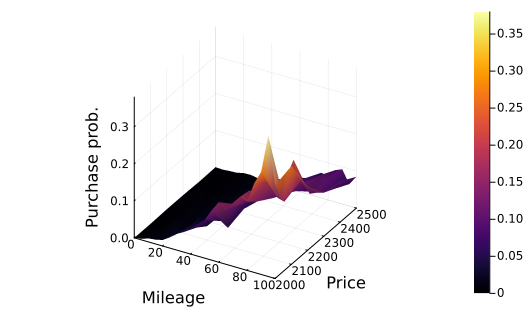
\includegraphics{./single_agent_dynamic_basic_files/figure-pdf/cell-24-output-1.svg}

}

\end{figure}

\hypertarget{section-27}{%
\section{4}\label{section-27}}

\begin{Shaded}
\begin{Highlighting}[]
\FunctionTok{transform!}\NormalTok{(}
    \FunctionTok{groupby}\NormalTok{(data\_gen, }\OperatorTok{:}\NormalTok{consumer\_id), }
\NormalTok{    [}\OperatorTok{:}\NormalTok{price, }\OperatorTok{:}\NormalTok{mileage, }\OperatorTok{:}\NormalTok{action] }\OperatorTok{.=\textgreater{}}\NormalTok{ ShiftedArrays.lag}
\NormalTok{    )}
\end{Highlighting}
\end{Shaded}

\begin{tabular}{r|ccccccccc}
    & state & action & period & consumer\_id & price & mileage & price\_lag & mileage\_lag & action\_lag\\
    \hline
    & Int64 & Int64 & Int64 & Int64 & Int64 & Int64 & Int64? & Int64? & Int64?\\
    \hline
    1 & 6 & 0 & 481 & 1 & 2500 & 0 & \emph{missing} & \emph{missing} & \emph{missing} \\
    2 & 12 & 0 & 482 & 1 & 2500 & 5 & 2500 & 0 & 0 \\
    3 & 18 & 0 & 483 & 1 & 2500 & 10 & 2500 & 5 & 0 \\
    4 & 14 & 0 & 484 & 1 & 2100 & 10 & 2500 & 10 & 0 \\
    5 & 25 & 0 & 485 & 1 & 2000 & 20 & 2100 & 10 & 0 \\
    6 & 28 & 0 & 486 & 1 & 2300 & 20 & 2000 & 20 & 0 \\
    7 & 28 & 0 & 487 & 1 & 2300 & 20 & 2300 & 20 & 0 \\
    8 & 27 & 0 & 488 & 1 & 2200 & 20 & 2300 & 20 & 0 \\
    9 & 27 & 0 & 489 & 1 & 2200 & 20 & 2200 & 20 & 0 \\
    10 & 34 & 0 & 490 & 1 & 2300 & 25 & 2200 & 20 & 0 \\
    11 & 31 & 0 & 491 & 1 & 2000 & 25 & 2300 & 25 & 0 \\
    12 & 32 & 0 & 492 & 1 & 2100 & 25 & 2000 & 25 & 0 \\
    13 & 34 & 0 & 493 & 1 & 2300 & 25 & 2100 & 25 & 0 \\
    14 & 35 & 0 & 494 & 1 & 2400 & 25 & 2300 & 25 & 0 \\
    15 & 35 & 0 & 495 & 1 & 2400 & 25 & 2400 & 25 & 0 \\
    16 & 35 & 0 & 496 & 1 & 2400 & 25 & 2400 & 25 & 0 \\
    17 & 35 & 0 & 497 & 1 & 2400 & 25 & 2400 & 25 & 0 \\
    18 & 35 & 0 & 498 & 1 & 2400 & 25 & 2400 & 25 & 0 \\
    19 & 35 & 0 & 499 & 1 & 2400 & 25 & 2400 & 25 & 0 \\
    20 & 34 & 0 & 500 & 1 & 2300 & 25 & 2400 & 25 & 0 \\
    21 & 34 & 0 & 501 & 1 & 2300 & 25 & 2300 & 25 & 0 \\
    22 & 34 & 0 & 502 & 1 & 2300 & 25 & 2300 & 25 & 0 \\
    23 & 33 & 0 & 503 & 1 & 2200 & 25 & 2300 & 25 & 0 \\
    24 & 34 & 0 & 504 & 1 & 2300 & 25 & 2200 & 25 & 0 \\
    25 & 46 & 0 & 505 & 1 & 2300 & 35 & 2300 & 25 & 0 \\
    26 & 46 & 0 & 506 & 1 & 2300 & 35 & 2300 & 35 & 0 \\
    27 & 48 & 0 & 507 & 1 & 2500 & 35 & 2300 & 35 & 0 \\
    28 & 45 & 0 & 508 & 1 & 2200 & 35 & 2500 & 35 & 0 \\
    29 & 51 & 0 & 509 & 1 & 2200 & 40 & 2200 & 35 & 0 \\
    30 & 57 & 0 & 510 & 1 & 2200 & 45 & 2200 & 40 & 0 \\
    $\dots$ & $\dots$ & $\dots$ & $\dots$ & $\dots$ & $\dots$ & $\dots$ & $\dots$ & $\dots$ & $\dots$ \\
\end{tabular}

\begin{Shaded}
\begin{Highlighting}[]
\FunctionTok{combine}\NormalTok{(}
    \FunctionTok{groupby}\NormalTok{(}
\NormalTok{        data\_gen }\OperatorTok{|\textgreater{}}
            \FunctionTok{filter}\NormalTok{(}\OperatorTok{:}\NormalTok{period }\OperatorTok{=\textgreater{}}\NormalTok{ (x }\OperatorTok{{-}\textgreater{}}\NormalTok{ x }\OperatorTok{!=}\NormalTok{ (num\_period }\OperatorTok{{-}}\NormalTok{ num\_period\_obs }\OperatorTok{+} \FloatTok{1}\NormalTok{))),}
\NormalTok{        [}\OperatorTok{:}\NormalTok{mileage\_lag, }\OperatorTok{:}\NormalTok{mileage, }\OperatorTok{:}\NormalTok{action\_lag]}
\NormalTok{    ),}
\NormalTok{    nrow}
\NormalTok{)}
\end{Highlighting}
\end{Shaded}

\begin{tabular}{r|cccc}
    & mileage\_lag & mileage & action\_lag & nrow\\
    \hline
    & Int64? & Int64 & Int64? & Int64\\
    \hline
    1 & 0 & 0 & 0 & 5725 \\
    2 & 0 & 0 & 1 & 4 \\
    3 & 0 & 5 & 0 & 2013 \\
    4 & 0 & 5 & 1 & 2 \\
    5 & 0 & 10 & 0 & 441 \\
    6 & 5 & 0 & 1 & 14 \\
    7 & 5 & 5 & 0 & 6858 \\
    8 & 5 & 5 & 1 & 1 \\
    9 & 5 & 10 & 0 & 2403 \\
    10 & 5 & 10 & 1 & 1 \\
    11 & 5 & 15 & 0 & 485 \\
    12 & 10 & 0 & 1 & 19 \\
    13 & 10 & 5 & 1 & 8 \\
    14 & 10 & 10 & 0 & 6612 \\
    15 & 10 & 10 & 1 & 1 \\
    16 & 10 & 15 & 0 & 2475 \\
    17 & 10 & 20 & 0 & 495 \\
    18 & 15 & 0 & 1 & 36 \\
    19 & 15 & 5 & 1 & 13 \\
    20 & 15 & 10 & 1 & 4 \\
    21 & 15 & 15 & 0 & 6665 \\
    22 & 15 & 20 & 0 & 2429 \\
    23 & 15 & 25 & 0 & 453 \\
    24 & 20 & 0 & 1 & 48 \\
    25 & 20 & 5 & 1 & 21 \\
    26 & 20 & 10 & 1 & 4 \\
    27 & 20 & 20 & 0 & 6445 \\
    28 & 20 & 25 & 0 & 2345 \\
    29 & 20 & 30 & 0 & 495 \\
    30 & 25 & 0 & 1 & 68 \\
    $\dots$ & $\dots$ & $\dots$ & $\dots$ & $\dots$ \\
\end{tabular}

\begin{Shaded}
\begin{Highlighting}[]
\NormalTok{num\_cond\_obs\_mileage }\OperatorTok{=} \FunctionTok{combine}\NormalTok{(}
    \FunctionTok{groupby}\NormalTok{(}
        \FunctionTok{transform}\NormalTok{(}
\NormalTok{            data\_gen }\OperatorTok{|\textgreater{}}
                \FunctionTok{filter}\NormalTok{(}\OperatorTok{:}\NormalTok{period }\OperatorTok{=\textgreater{}}\NormalTok{ (x }\OperatorTok{{-}\textgreater{}}\NormalTok{ x }\OperatorTok{!=}\NormalTok{ (num\_period }\OperatorTok{{-}}\NormalTok{ num\_period\_obs }\OperatorTok{+} \FloatTok{1}\NormalTok{))),}
\NormalTok{            [}\OperatorTok{:}\NormalTok{mileage\_lag, }\OperatorTok{:}\NormalTok{mileage, }\OperatorTok{:}\NormalTok{action\_lag] }\OperatorTok{=\textgreater{}}
            \FunctionTok{ByRow}\NormalTok{(}
\NormalTok{                (mileage\_lag, mileage, action\_lag) }\OperatorTok{{-}\textgreater{}}
\NormalTok{                (}
\NormalTok{                    ((action\_lag }\OperatorTok{==} \FloatTok{0}\NormalTok{) }\OperatorTok{\&}\NormalTok{ (}\FloatTok{5} \OperatorTok{\textless{}=}\NormalTok{ mileage\_lag }\OperatorTok{\textless{}=} \FloatTok{95}\NormalTok{) }\OperatorTok{\&}\NormalTok{ (mileage\_lag }\OperatorTok{==}\NormalTok{ mileage)) }\OperatorTok{|}
\NormalTok{                    ((action\_lag }\OperatorTok{==} \FloatTok{1}\NormalTok{) }\OperatorTok{\&}\NormalTok{ (mileage }\OperatorTok{==} \FloatTok{0}\NormalTok{))}
\NormalTok{                    ) ? }\StringTok{"cond\_obs\_mileage1"} \OperatorTok{:}
\NormalTok{                (}
\NormalTok{                    ((action\_lag }\OperatorTok{==} \FloatTok{0}\NormalTok{) }\OperatorTok{\&}\NormalTok{ (}\FloatTok{5} \OperatorTok{\textless{}=}\NormalTok{ mileage\_lag }\OperatorTok{\textless{}=} \FloatTok{90}\NormalTok{) }\OperatorTok{\&}\NormalTok{ (mileage\_lag }\OperatorTok{==}\NormalTok{ mileage }\OperatorTok{{-}} \FloatTok{5}\NormalTok{)) }\OperatorTok{|}
\NormalTok{                    ((action\_lag }\OperatorTok{==} \FloatTok{1}\NormalTok{) }\OperatorTok{\&}\NormalTok{ (mileage }\OperatorTok{==} \FloatTok{5}\NormalTok{))}
\NormalTok{                    ) ? }\StringTok{"cond\_obs\_mileage2"} \OperatorTok{:}
\NormalTok{                (}
\NormalTok{                    ((action\_lag }\OperatorTok{==} \FloatTok{0}\NormalTok{) }\OperatorTok{\&}\NormalTok{ (}\FloatTok{5} \OperatorTok{\textless{}=}\NormalTok{ mileage\_lag }\OperatorTok{\textless{}=} \FloatTok{90}\NormalTok{) }\OperatorTok{\&}\NormalTok{ (mileage\_lag }\OperatorTok{==}\NormalTok{ mileage }\OperatorTok{{-}} \FloatTok{10}\NormalTok{)) }\OperatorTok{|}
\NormalTok{                    ((action\_lag }\OperatorTok{==} \FloatTok{1}\NormalTok{) }\OperatorTok{\&}\NormalTok{ (mileage }\OperatorTok{==} \FloatTok{10}\NormalTok{))}
\NormalTok{                    ) ? }\StringTok{"cond\_obs\_mileage3"} \OperatorTok{:}
\NormalTok{                (}
\NormalTok{                    ((action\_lag }\OperatorTok{==} \FloatTok{0}\NormalTok{) }\OperatorTok{\&}\NormalTok{ (mileage\_lag }\OperatorTok{==} \FloatTok{95}\NormalTok{) }\OperatorTok{\&}\NormalTok{ (mileage }\OperatorTok{==} \FloatTok{100}\NormalTok{))}
\NormalTok{                    ) ? }\StringTok{"cond\_obs\_mileage4"} \OperatorTok{:}
                \StringTok{"other"}
\NormalTok{            ) }\OperatorTok{=\textgreater{}}
            \OperatorTok{:}\NormalTok{cond\_obs\_mileage}
\NormalTok{            ),}
\NormalTok{        [}\OperatorTok{:}\NormalTok{cond\_obs\_mileage]}
\NormalTok{        ),}
\NormalTok{    nrow }\OperatorTok{=\textgreater{}} \OperatorTok{:}\NormalTok{num\_cond\_obs}
\NormalTok{) }\OperatorTok{|\textgreater{}} \FunctionTok{filter}\NormalTok{(}\OperatorTok{:}\NormalTok{cond\_obs\_mileage }\OperatorTok{=\textgreater{}}\NormalTok{ (x }\OperatorTok{{-}\textgreater{}}\NormalTok{ (x }\OperatorTok{!=} \StringTok{"other"}\NormalTok{)));}

\NormalTok{num\_cond\_obs\_mileage }\OperatorTok{=} \FunctionTok{Dict}\NormalTok{(}
\NormalTok{    k }\OperatorTok{=\textgreater{}}\NormalTok{ v[}\FloatTok{1}\NormalTok{, }\StringTok{"num\_cond\_obs"}\NormalTok{] }
    \ControlFlowTok{for}\NormalTok{ ((k, ), v) }\KeywordTok{in} \FunctionTok{pairs}\NormalTok{(}\FunctionTok{groupby}\NormalTok{(num\_cond\_obs\_mileage, }\OperatorTok{:}\NormalTok{cond\_obs\_mileage))}
\NormalTok{    );}
\end{Highlighting}
\end{Shaded}

\begin{Shaded}
\begin{Highlighting}[]
\NormalTok{kappa\_est }\OperatorTok{=} \FunctionTok{zeros}\NormalTok{(}\FloatTok{2}\NormalTok{);}

\NormalTok{kappa\_est[}\FloatTok{1}\NormalTok{] }\OperatorTok{=}\NormalTok{ num\_cond\_obs\_mileage[}\StringTok{"cond\_obs\_mileage2"}\NormalTok{] }\OperatorTok{*}\NormalTok{ (}
\NormalTok{    num\_cond\_obs\_mileage[}\StringTok{"cond\_obs\_mileage2"}\NormalTok{] }\OperatorTok{+}
\NormalTok{    num\_cond\_obs\_mileage[}\StringTok{"cond\_obs\_mileage3"}\NormalTok{] }\OperatorTok{+}
\NormalTok{    num\_cond\_obs\_mileage[}\StringTok{"cond\_obs\_mileage4"}\NormalTok{]}
\NormalTok{) }\OperatorTok{/}\NormalTok{ (}
\NormalTok{    (num\_cond\_obs\_mileage[}\StringTok{"cond\_obs\_mileage2"}\NormalTok{] }\OperatorTok{+}\NormalTok{ num\_cond\_obs\_mileage[}\StringTok{"cond\_obs\_mileage3"}\NormalTok{]) }\OperatorTok{*}\NormalTok{ (}
\NormalTok{    num\_cond\_obs\_mileage[}\StringTok{"cond\_obs\_mileage1"}\NormalTok{] }\OperatorTok{+}
\NormalTok{    num\_cond\_obs\_mileage[}\StringTok{"cond\_obs\_mileage2"}\NormalTok{] }\OperatorTok{+}
\NormalTok{    num\_cond\_obs\_mileage[}\StringTok{"cond\_obs\_mileage3"}\NormalTok{] }\OperatorTok{+}
\NormalTok{    num\_cond\_obs\_mileage[}\StringTok{"cond\_obs\_mileage4"}\NormalTok{]}
\NormalTok{    )}
\NormalTok{);}

\NormalTok{kappa\_est[}\FloatTok{2}\NormalTok{] }\OperatorTok{=}\NormalTok{ num\_cond\_obs\_mileage[}\StringTok{"cond\_obs\_mileage3"}\NormalTok{] }\OperatorTok{*}\NormalTok{ (}
\NormalTok{    num\_cond\_obs\_mileage[}\StringTok{"cond\_obs\_mileage2"}\NormalTok{] }\OperatorTok{+}
\NormalTok{    num\_cond\_obs\_mileage[}\StringTok{"cond\_obs\_mileage3"}\NormalTok{] }\OperatorTok{+}
\NormalTok{    num\_cond\_obs\_mileage[}\StringTok{"cond\_obs\_mileage4"}\NormalTok{]}
\NormalTok{) }\OperatorTok{/}\NormalTok{ (}
\NormalTok{    (num\_cond\_obs\_mileage[}\StringTok{"cond\_obs\_mileage2"}\NormalTok{] }\OperatorTok{+}\NormalTok{ num\_cond\_obs\_mileage[}\StringTok{"cond\_obs\_mileage3"}\NormalTok{]) }\OperatorTok{*}\NormalTok{ (}
\NormalTok{    num\_cond\_obs\_mileage[}\StringTok{"cond\_obs\_mileage1"}\NormalTok{] }\OperatorTok{+}
\NormalTok{    num\_cond\_obs\_mileage[}\StringTok{"cond\_obs\_mileage2"}\NormalTok{] }\OperatorTok{+}
\NormalTok{    num\_cond\_obs\_mileage[}\StringTok{"cond\_obs\_mileage3"}\NormalTok{] }\OperatorTok{+}
\NormalTok{    num\_cond\_obs\_mileage[}\StringTok{"cond\_obs\_mileage4"}\NormalTok{]}
\NormalTok{    )}
\NormalTok{);}

\NormalTok{kappa\_est}
\end{Highlighting}
\end{Shaded}

\begin{verbatim}
2-element Vector{Float64}:
 0.2507060588583926
 0.05038686722769128
\end{verbatim}

\begin{Shaded}
\begin{Highlighting}[]
\NormalTok{Infomat\_mileage\_est }\OperatorTok{=} \FunctionTok{zeros}\NormalTok{((}\FloatTok{2}\NormalTok{, }\FloatTok{2}\NormalTok{));}

\NormalTok{Infomat\_mileage\_est[}\FloatTok{1}\NormalTok{, }\FloatTok{1}\NormalTok{] }\OperatorTok{=}\NormalTok{ (}
\NormalTok{    (num\_cond\_obs\_mileage[}\StringTok{"cond\_obs\_mileage1"}\NormalTok{] }\OperatorTok{/}\NormalTok{ (}\FloatTok{1} \OperatorTok{{-}}\NormalTok{ kappa\_est[}\FloatTok{1}\NormalTok{] }\OperatorTok{{-}}\NormalTok{ kappa\_est[}\FloatTok{2}\NormalTok{])}\OperatorTok{\^{}}\FloatTok{2}\NormalTok{) }\OperatorTok{+}
\NormalTok{    (num\_cond\_obs\_mileage[}\StringTok{"cond\_obs\_mileage2"}\NormalTok{] }\OperatorTok{/}\NormalTok{ kappa\_est[}\FloatTok{1}\NormalTok{]}\OperatorTok{\^{}}\FloatTok{2}\NormalTok{) }\OperatorTok{+}
\NormalTok{    (num\_cond\_obs\_mileage[}\StringTok{"cond\_obs\_mileage4"}\NormalTok{] }\OperatorTok{/}\NormalTok{ (kappa\_est[}\FloatTok{1}\NormalTok{] }\OperatorTok{+}\NormalTok{ kappa\_est[}\FloatTok{2}\NormalTok{])}\OperatorTok{\^{}}\FloatTok{2}\NormalTok{)}
\NormalTok{);}

\NormalTok{Infomat\_mileage\_est[}\FloatTok{1}\NormalTok{, }\FloatTok{2}\NormalTok{] }\OperatorTok{=}\NormalTok{ (}
\NormalTok{    (num\_cond\_obs\_mileage[}\StringTok{"cond\_obs\_mileage1"}\NormalTok{] }\OperatorTok{/}\NormalTok{ (}\FloatTok{1} \OperatorTok{{-}}\NormalTok{ kappa\_est[}\FloatTok{1}\NormalTok{] }\OperatorTok{{-}}\NormalTok{ kappa\_est[}\FloatTok{2}\NormalTok{])}\OperatorTok{\^{}}\FloatTok{2}\NormalTok{) }\OperatorTok{+}
\NormalTok{    (num\_cond\_obs\_mileage[}\StringTok{"cond\_obs\_mileage4"}\NormalTok{] }\OperatorTok{/}\NormalTok{ (kappa\_est[}\FloatTok{1}\NormalTok{] }\OperatorTok{+}\NormalTok{ kappa\_est[}\FloatTok{2}\NormalTok{])}\OperatorTok{\^{}}\FloatTok{2}\NormalTok{)}
\NormalTok{);}

\NormalTok{Infomat\_mileage\_est[}\FloatTok{2}\NormalTok{, }\FloatTok{1}\NormalTok{] }\OperatorTok{=}\NormalTok{ Infomat\_mileage\_est[}\FloatTok{1}\NormalTok{, }\FloatTok{2}\NormalTok{];}

\NormalTok{Infomat\_mileage\_est[}\FloatTok{2}\NormalTok{, }\FloatTok{2}\NormalTok{] }\OperatorTok{=}\NormalTok{ (}
\NormalTok{    (num\_cond\_obs\_mileage[}\StringTok{"cond\_obs\_mileage1"}\NormalTok{] }\OperatorTok{/}\NormalTok{ (}\FloatTok{1} \OperatorTok{{-}}\NormalTok{ kappa\_est[}\FloatTok{1}\NormalTok{] }\OperatorTok{{-}}\NormalTok{ kappa\_est[}\FloatTok{2}\NormalTok{])}\OperatorTok{\^{}}\FloatTok{2}\NormalTok{) }\OperatorTok{+}
\NormalTok{    (num\_cond\_obs\_mileage[}\StringTok{"cond\_obs\_mileage3"}\NormalTok{] }\OperatorTok{/}\NormalTok{ kappa\_est[}\FloatTok{2}\NormalTok{]}\OperatorTok{\^{}}\FloatTok{2}\NormalTok{) }\OperatorTok{+}
\NormalTok{    (num\_cond\_obs\_mileage[}\StringTok{"cond\_obs\_mileage4"}\NormalTok{] }\OperatorTok{/}\NormalTok{ (kappa\_est[}\FloatTok{1}\NormalTok{] }\OperatorTok{+}\NormalTok{ kappa\_est[}\FloatTok{2}\NormalTok{])}\OperatorTok{\^{}}\FloatTok{2}\NormalTok{)}
\NormalTok{);}

\NormalTok{kappa\_se }\OperatorTok{=} \FunctionTok{sqrt}\NormalTok{.(}\FunctionTok{diag}\NormalTok{(}\FunctionTok{inv}\NormalTok{(Infomat\_mileage\_est)));}
\end{Highlighting}
\end{Shaded}

\begin{Shaded}
\begin{Highlighting}[]
\FunctionTok{DataFrame}\NormalTok{(kappa\_est }\OperatorTok{=}\NormalTok{ kappa\_est, kappa\_se }\OperatorTok{=}\NormalTok{ kappa\_se)}
\end{Highlighting}
\end{Shaded}

\begin{tabular}{r|cc}
    & kappa\_est & kappa\_se\\
    \hline
    & Float64 & Float64\\
    \hline
    1 & 0.250706 & 0.0013098 \\
    2 & 0.0503869 & 0.000662066 \\
\end{tabular}

\begin{Shaded}
\begin{Highlighting}[]
\NormalTok{num\_cond\_obs\_price }\OperatorTok{=} \FunctionTok{combine}\NormalTok{(}
    \FunctionTok{groupby}\NormalTok{(}
\NormalTok{        data\_gen }\OperatorTok{|\textgreater{}}
            \FunctionTok{filter}\NormalTok{(}\OperatorTok{:}\NormalTok{period }\OperatorTok{=\textgreater{}}\NormalTok{ (x }\OperatorTok{{-}\textgreater{}}\NormalTok{ x }\OperatorTok{!=}\NormalTok{ (num\_period }\OperatorTok{{-}}\NormalTok{ num\_period\_obs }\OperatorTok{+} \FloatTok{1}\NormalTok{))),}
\NormalTok{        [}\OperatorTok{:}\NormalTok{price\_lag, }\OperatorTok{:}\NormalTok{price]}
\NormalTok{    ),}
\NormalTok{    nrow }\OperatorTok{=\textgreater{}} \OperatorTok{:}\NormalTok{num\_cond\_obs}
\NormalTok{)}

\NormalTok{num\_cond\_obs\_price }\OperatorTok{=}\NormalTok{ [}
\NormalTok{    (}
\NormalTok{        num\_cond\_obs\_price }\OperatorTok{|\textgreater{}} 
            \FunctionTok{filter}\NormalTok{([}\OperatorTok{:}\NormalTok{price\_lag, }\OperatorTok{:}\NormalTok{price] }\OperatorTok{=\textgreater{}}\NormalTok{ ((price\_lag, price) }\OperatorTok{{-}\textgreater{}}\NormalTok{ ((price\_lag }\OperatorTok{==}\NormalTok{ p\_lag) }\OperatorTok{\&}\NormalTok{ (price }\OperatorTok{==}\NormalTok{ p))))}
\NormalTok{    )[}\FloatTok{1}\NormalTok{, }\OperatorTok{:}\NormalTok{num\_cond\_obs]}
\NormalTok{    for p\_lag }\KeywordTok{in}\NormalTok{ price\_states, p }\KeywordTok{in}\NormalTok{ price\_states}
\NormalTok{]}

\NormalTok{lambda\_est\_mat }\OperatorTok{=}\NormalTok{ num\_cond\_obs\_price }\OperatorTok{./} \FunctionTok{sum}\NormalTok{(num\_cond\_obs\_price, dims }\OperatorTok{=} \FloatTok{2}\NormalTok{)}
\end{Highlighting}
\end{Shaded}

\begin{verbatim}
6×6 Matrix{Float64}:
 0.0992722  0.101205   0.196952  0.198431  0.205254  0.198886
 0.104459   0.10081    0.200023  0.201733  0.20447   0.188505
 0.0998312  0.0979389  0.29888   0.205646  0.197719  0.0999847
 0.101128   0.098588   0.197836  0.300843  0.200477  0.101128
 0.0495297  0.0498236  0.1       0.100911  0.50047   0.199265
 0.0486584  0.0509654  0.103705  0.100511  0.198112  0.498048
\end{verbatim}

\begin{Shaded}
\begin{Highlighting}[]
\CommentTok{\# TODO}
\NormalTok{lambda\_se }\OperatorTok{=} \FunctionTok{zeros}\NormalTok{(num\_price\_states)}
\end{Highlighting}
\end{Shaded}

\begin{verbatim}
6-element Vector{Float64}:
 0.0
 0.0
 0.0
 0.0
 0.0
 0.0
\end{verbatim}

\begin{Shaded}
\begin{Highlighting}[]
\NormalTok{lambda\_est }\OperatorTok{=}\NormalTok{ lambda\_est\_mat}\OperatorTok{\textquotesingle{}}\NormalTok{[lambda\_est\_mat}\OperatorTok{\textquotesingle{}} \OperatorTok{.!=} \FunctionTok{diag}\NormalTok{(lambda\_est\_mat)]}
\end{Highlighting}
\end{Shaded}

\begin{verbatim}
30-element Vector{Float64}:
 0.10120536729588356
 0.1969524675915397
 0.19843074823743462
 0.2052535819877189
 0.1988856038207869
 0.10445888926901585
 0.20002280761774432
 0.20173337894856883
 0.20447029307788803
 0.1885049606568594
 0.09983122794456094
 0.09793893520175932
 0.2056461924001432
 ⋮
 0.20047744819179195
 0.10112759041040227
 0.04952968841857731
 0.04982363315696649
 0.1
 0.10091122868900647
 0.19926513815402705
 0.04865843270868825
 0.050965360590573536
 0.1037052810902896
 0.10051107325383304
 0.19811186825667235
\end{verbatim}

\hypertarget{section-28}{%
\section{5}\label{section-28}}

\begin{Shaded}
\begin{Highlighting}[]
\KeywordTok{function} \FunctionTok{logLH\_stat}\NormalTok{(}
\NormalTok{    theta,}
\NormalTok{    states\_matrix}\OperatorTok{::}\DataTypeTok{Matrix\{Int\}}\NormalTok{,}
\NormalTok{    data\_gen}\OperatorTok{::}\DataTypeTok{DataFrame}
\NormalTok{)}
\NormalTok{    U }\OperatorTok{=} \FunctionTok{flow\_utility}\NormalTok{(theta, states\_matrix);}
\NormalTok{    prob\_C\_stat }\OperatorTok{=} \FunctionTok{exp}\NormalTok{.(U) }\OperatorTok{./} \FunctionTok{sum}\NormalTok{(}\FunctionTok{exp}\NormalTok{.(U), dims }\OperatorTok{=} \FloatTok{2}\NormalTok{);}
    \ControlFlowTok{return} \FunctionTok{sum}\NormalTok{(}\FunctionTok{log}\NormalTok{.([prob\_C\_stat[x.state, x.action }\OperatorTok{+} \FloatTok{1}\NormalTok{] for x }\KeywordTok{in} \FunctionTok{eachrow}\NormalTok{(data\_gen)]))}
\KeywordTok{end}
\end{Highlighting}
\end{Shaded}

\begin{verbatim}
logLH_stat (generic function with 1 method)
\end{verbatim}

\begin{Shaded}
\begin{Highlighting}[]
\NormalTok{objFunc\_for\_Optim\_stat }\OperatorTok{=} \FunctionTok{TwiceDifferentiable}\NormalTok{(}
\NormalTok{    x }\OperatorTok{{-}\textgreater{}} \OperatorTok{{-}} \FunctionTok{logLH\_stat}\NormalTok{(x, states\_matrix, data\_gen),}
\NormalTok{    theta\_true;}
\NormalTok{    autodiff }\OperatorTok{=} \OperatorTok{:}\NormalTok{forward}
\NormalTok{    );}

\PreprocessorTok{@time}\NormalTok{ logit\_stat\_opt }\OperatorTok{=} \FunctionTok{optimize}\NormalTok{(}
\NormalTok{    objFunc\_for\_Optim\_stat,}
\NormalTok{    theta\_true,}
\NormalTok{    Optim.}\FunctionTok{Options}\NormalTok{(show\_trace }\OperatorTok{=} \ConstantTok{true}\NormalTok{)}
\NormalTok{)}
\end{Highlighting}
\end{Shaded}

\begin{verbatim}
Iter     Function value   Gradient norm 
     0     2.297333e+04     7.561388e+06
\end{verbatim}

\begin{verbatim}
 * time: 0.007976055145263672
\end{verbatim}

\begin{verbatim}
     1     1.468656e+04     3.971824e+06
 * time: 0.34108710289001465
\end{verbatim}

\begin{verbatim}
     2     1.407678e+04     3.143506e+06
 * time: 0.40247201919555664
\end{verbatim}

\begin{verbatim}
     3     1.355774e+04     1.214883e+06
 * time: 0.46057891845703125
\end{verbatim}

\begin{verbatim}
     4     1.350421e+04     2.487112e+04
 * time: 0.5168969631195068
\end{verbatim}

\begin{verbatim}
     5     1.350416e+04     2.355812e+01
 * time: 0.5752720832824707
\end{verbatim}

\begin{verbatim}
     6     1.350416e+04     7.915900e-06
 * time: 0.6456060409545898
\end{verbatim}

\begin{verbatim}
     7     1.350416e+04     3.805326e-09
 * time: 0.7008991241455078
\end{verbatim}

\begin{verbatim}
  2.427718 seconds (23.67 M allocations: 987.043 MiB, 6.72% gc time, 80.65% compilation time)
\end{verbatim}

\begin{verbatim}
 * Status: success

 * Candidate solution
    Final objective value:     1.350416e+04

 * Found with
    Algorithm:     Newton's Method

 * Convergence measures
    |x - x'|               = 5.38e-14 ≰ 0.0e+00
    |x - x'|/|x'|          = 1.26e-12 ≰ 0.0e+00
    |f(x) - f(x')|         = 1.82e-12 ≰ 0.0e+00
    |f(x) - f(x')|/|f(x')| = 1.35e-16 ≰ 0.0e+00
    |g(x)|                 = 3.81e-09 ≤ 1.0e-08

 * Work counters
    Seconds run:   1  (vs limit Inf)
    Iterations:    7
    f(x) calls:    17
    ∇f(x) calls:   17
    ∇²f(x) calls:  7
\end{verbatim}

\begin{Shaded}
\begin{Highlighting}[]
\NormalTok{theta\_est\_stat }\OperatorTok{=}\NormalTok{ logit\_stat\_opt.minimizer;}

\NormalTok{hessian\_stat }\OperatorTok{=}\NormalTok{ ForwardDiff.}\FunctionTok{hessian}\NormalTok{(}
\NormalTok{    x }\OperatorTok{{-}\textgreater{}} \OperatorTok{{-}} \FunctionTok{logLH\_stat}\NormalTok{(x, states\_matrix, data\_gen),}
\NormalTok{    logit\_stat\_opt.minimizer}
\NormalTok{    );}

\NormalTok{theta\_se\_stat }\OperatorTok{=} \FunctionTok{sqrt}\NormalTok{.(}\FunctionTok{diag}\NormalTok{(}\FunctionTok{inv}\NormalTok{(hessian\_stat)));}
\end{Highlighting}
\end{Shaded}

\begin{Shaded}
\begin{Highlighting}[]
\FunctionTok{DataFrame}\NormalTok{(theta\_est\_stat }\OperatorTok{=}\NormalTok{ theta\_est\_stat, theta\_se\_stat }\OperatorTok{=}\NormalTok{ theta\_se\_stat)}
\end{Highlighting}
\end{Shaded}

\begin{tabular}{r|cc}
    & theta\_est\_stat & theta\_se\_stat\\
    \hline
    & Float64 & Float64\\
    \hline
    1 & 0.0428171 & 0.000692099 \\
    2 & 0.00237647 & 1.9178e-5 \\
\end{tabular}

\hypertarget{section-29}{%
\subsection{5.2}\label{section-29}}

\begin{Shaded}
\begin{Highlighting}[]
\NormalTok{mileage\_trans\_mat\_hat }\OperatorTok{=} \FunctionTok{zeros}\NormalTok{((num\_mileage\_states, num\_mileage\_states, num\_choice));}
\FunctionTok{gen\_mileage\_trans!}\NormalTok{(kappa\_est, num\_mileage\_states, mileage\_trans\_mat\_hat);}

\NormalTok{price\_trans\_mat\_hat }\OperatorTok{=} \FunctionTok{zeros}\NormalTok{(num\_price\_states, num\_price\_states);}
\FunctionTok{gen\_price\_trans!}\NormalTok{(lambda\_est, num\_price\_states, price\_trans\_mat\_hat);}

\NormalTok{trans\_mat\_hat }\OperatorTok{=} \FunctionTok{Array}\DataTypeTok{\{Float64\}}\NormalTok{(}\ConstantTok{undef}\NormalTok{, num\_states, num\_states, num\_choice);}
\ControlFlowTok{for}\NormalTok{ i }\KeywordTok{in} \FloatTok{1}\OperatorTok{:}\NormalTok{num\_choice}
\NormalTok{    trans\_mat\_hat[}\OperatorTok{:}\NormalTok{, }\OperatorTok{:}\NormalTok{, i] }\OperatorTok{=} \FunctionTok{kron}\NormalTok{(mileage\_trans\_mat\_hat[}\OperatorTok{:}\NormalTok{, }\OperatorTok{:}\NormalTok{, i], price\_trans\_mat\_hat);}
\ControlFlowTok{end}
\end{Highlighting}
\end{Shaded}

\begin{Shaded}
\begin{Highlighting}[]
\KeywordTok{function} \FunctionTok{logLH}\NormalTok{(}
\NormalTok{    theta,}
\NormalTok{    beta}\OperatorTok{::}\DataTypeTok{Float64}\NormalTok{,}
\NormalTok{    trans\_mat}\OperatorTok{::}\DataTypeTok{Array\{Float64, 3\}}\NormalTok{,}
\NormalTok{    states\_matrix}\OperatorTok{::}\DataTypeTok{Matrix\{Int\}}\NormalTok{,}
\NormalTok{    data\_gen}\OperatorTok{::}\DataTypeTok{DataFrame}
\NormalTok{)}

\NormalTok{    EV }\OperatorTok{=} \FunctionTok{contraction}\NormalTok{(theta, beta, trans\_mat, states\_matrix);}
    
\NormalTok{    U }\OperatorTok{=} \FunctionTok{flow\_utility}\NormalTok{(theta, states\_matrix);}
\NormalTok{    V\_CS }\OperatorTok{=}\NormalTok{ U }\OperatorTok{+}\NormalTok{ beta }\OperatorTok{.*}\NormalTok{ EV;}

\NormalTok{    prob\_C }\OperatorTok{=} \FunctionTok{exp}\NormalTok{.(V\_CS) }\OperatorTok{./} \FunctionTok{sum}\NormalTok{(}\FunctionTok{exp}\NormalTok{.(V\_CS), dims }\OperatorTok{=} \FloatTok{2}\NormalTok{);}

    \ControlFlowTok{return} \FunctionTok{sum}\NormalTok{(}\FunctionTok{log}\NormalTok{.([prob\_C[x.state, x.action }\OperatorTok{+} \FloatTok{1}\NormalTok{] for x }\KeywordTok{in} \FunctionTok{eachrow}\NormalTok{(data\_gen)]))}
\KeywordTok{end}
\end{Highlighting}
\end{Shaded}

\begin{verbatim}
logLH (generic function with 1 method)
\end{verbatim}

\begin{Shaded}
\begin{Highlighting}[]
\NormalTok{objFunc\_for\_Optim }\OperatorTok{=} \FunctionTok{TwiceDifferentiable}\NormalTok{(}
\NormalTok{    x }\OperatorTok{{-}\textgreater{}} \OperatorTok{{-}} \FunctionTok{logLH}\NormalTok{(x, beta, trans\_mat\_hat, states\_matrix, data\_gen),}
\NormalTok{    theta\_true;}
\NormalTok{    autodiff }\OperatorTok{=} \OperatorTok{:}\NormalTok{forward}
\NormalTok{    );}

\PreprocessorTok{@time}\NormalTok{ NFXP\_opt }\OperatorTok{=} \FunctionTok{optimize}\NormalTok{(}
\NormalTok{    objFunc\_for\_Optim,}
\NormalTok{    theta\_true,}
\NormalTok{    Optim.}\FunctionTok{Options}\NormalTok{(show\_trace }\OperatorTok{=} \ConstantTok{true}\NormalTok{)}
\NormalTok{)}
\end{Highlighting}
\end{Shaded}

\begin{verbatim}
Iter     Function value   Gradient norm 
     0     1.333725e+04     5.946862e+03
 * time: 8.296966552734375e-5
\end{verbatim}

\begin{verbatim}
     1     1.333722e+04     3.170489e+00
 * time: 1.3130271434783936
\end{verbatim}

\begin{verbatim}
     2     1.333722e+04     4.639569e-07
 * time: 2.6059720516204834
\end{verbatim}

\begin{verbatim}
     3     1.333722e+04     3.080640e-08
 * time: 3.594815969467163
\end{verbatim}

\begin{verbatim}
     4     1.333722e+04     4.640242e-08
 * time: 4.647303104400635
\end{verbatim}

\begin{verbatim}
     5     1.333722e+04     3.628702e-08
 * time: 5.704677104949951
\end{verbatim}

\begin{verbatim}
     6     1.333722e+04     6.017217e-09
 * time: 6.325474977493286
\end{verbatim}

\begin{verbatim}
  9.609289 seconds (25.64 M allocations: 22.485 GiB, 15.36% gc time, 26.21% compilation time)
\end{verbatim}

\begin{verbatim}
 * Status: success (objective increased between iterations)

 * Candidate solution
    Final objective value:     1.333722e+04

 * Found with
    Algorithm:     Newton's Method

 * Convergence measures
    |x - x'|               = 9.54e-18 ≰ 0.0e+00
    |x - x'|/|x'|          = 2.37e-15 ≰ 0.0e+00
    |f(x) - f(x')|         = 1.82e-12 ≰ 0.0e+00
    |f(x) - f(x')|/|f(x')| = 1.36e-16 ≰ 0.0e+00
    |g(x)|                 = 6.02e-09 ≤ 1.0e-08

 * Work counters
    Seconds run:   6  (vs limit Inf)
    Iterations:    6
    f(x) calls:    15
    ∇f(x) calls:   15
    ∇²f(x) calls:  6
\end{verbatim}

\begin{Shaded}
\begin{Highlighting}[]
\NormalTok{theta\_est }\OperatorTok{=}\NormalTok{ NFXP\_opt.minimizer;}

\NormalTok{hessian }\OperatorTok{=}\NormalTok{ ForwardDiff.}\FunctionTok{hessian}\NormalTok{(}
\NormalTok{    x }\OperatorTok{{-}\textgreater{}} \OperatorTok{{-}} \FunctionTok{logLH}\NormalTok{(x, beta, trans\_mat\_hat, states\_matrix, data\_gen),}
\NormalTok{    NFXP\_opt.minimizer}
\NormalTok{    );}

\NormalTok{theta\_se }\OperatorTok{=} \FunctionTok{sqrt}\NormalTok{.(}\FunctionTok{diag}\NormalTok{(}\FunctionTok{inv}\NormalTok{(hessian)));}
\end{Highlighting}
\end{Shaded}

\begin{Shaded}
\begin{Highlighting}[]
\FunctionTok{DataFrame}\NormalTok{(theta\_est }\OperatorTok{=}\NormalTok{ theta\_est, theta\_se }\OperatorTok{=}\NormalTok{ theta\_se)}
\end{Highlighting}
\end{Shaded}

\begin{tabular}{r|cc}
    & theta\_est & theta\_se\\
    \hline
    & Float64 & Float64\\
    \hline
    1 & 0.00401826 & 8.88337e-5 \\
    2 & 0.00300455 & 3.67953e-5 \\
\end{tabular}



\end{document}
